% ******************************* PhD Thesis Template **************************
% Please have a look at the README.md file for info on how to use the template

\documentclass[a4paper,fonsize=12pt,custommargin,numbered,print,index]{PhDThesisPSnPDF}

% ******************************************************************************
% ******************************* Class Options ********************************
% *********************** See README for more details **************************
% ******************************************************************************

% `a4paper'(The University of Cambridge PhD thesis guidelines recommends a page
% size a4 - default option) or `a5paper': A5 Paper size is also allowed as per
% the Cambridge University Engineering Deparment guidelines for PhD thesis
%
% `11pt' or `12pt'(default): Font Size 10pt is NOT recommended by the University
% guidelines
%
% `oneside' or `twoside'(default): Printing double side (twoside) or single
% side.
%
% `print': Use `print' for print version with appropriate margins and page
% layout. Leaving the options field blank will activate Online version.
%
% `index': For index at the end of the thesis
%
% `draftclassic': For draft mode without loading any images (same as draft in book)
%
% `draft': Special draft mode with line numbers, images, and water mark with
% timestamp and custom text. Position of the text can also be modified.
%
% `abstract': To generate only the title page and abstract page with
% dissertation title and name, to submit to the Student Registry
%
% `chapter`: This option enables only the specified chapter and its references
%  Useful for review and corrections.
%
% ************************* Custom Page Margins ********************************
%
% `custommargin`: Use `custommargin' in options to activate custom page margins,
% which can be defined in the preamble.tex. Custom margin will override
% print/online margin setup.
%
% *********************** Choosing the Fonts in Class Options ******************
%
% `times' : Times font with math support. (The Cambridge University guidelines
% recommend using times)
%
% `fourier': Utopia Font with Fourier Math font (Font has to be installed)
%            It's a free font.
%
% `customfont': Use `customfont' option in the document class and load the
% package in the preamble.tex
%
% default or leave empty: `Latin Modern' font will be loaded.
%
% ********************** Choosing the Bibliography style ***********************
%
% `authoryear': For author-year citation eg., Krishna (2013)
%
% `numbered': (Default Option) For numbered and sorted citation e.g., [1,5,2]
%
% `custombib': Define your own bibliography style in the `preamble.tex' file.
%              `\RequirePackage[square, sort, numbers, authoryear]{natbib}'.
%              This can be also used to load biblatex instead of natbib
%              (See Preamble)
%
% **************************** Choosing the Page Style *************************
%
% `default (leave empty)': For Page Numbers in Header (Left Even, Right Odd) and
% Chapter Name in Header (Right Even) and Section Name (Left Odd). Blank Footer.
%
% `PageStyleI': Chapter Name next & Page Number on Even Side (Left Even).
% Section Name & Page Number in Header on Odd Side (Right Odd). Footer is empty.
%
% `PageStyleII': Chapter Name on Even Side (Left Even) in Header. Section Number
% and Section Name in Header on Odd Side (Right Odd). Page numbering in footer

% Uncomment to change page style
%\pagestyle{PageStyleII}

% ********************************** Preamble **********************************
% Preamble: Contains packages and user-defined commands and settings
% ******************************************************************************
% ****************************** Custom Margin *********************************

% Add `custommargin' in the document class options to use this section
% Set {innerside margin / outerside margin / topmargin / bottom margin}  and
% other page dimensions
\ifsetCustomMargin
\RequirePackage[left=37mm,right=30mm,top=35mm,bottom=30mm]{geometry}
  \setFancyHdr % To apply fancy header after geometry package is loaded
\fi

% Add spaces between paragraphs
%\setlength{\parskip}{0.5em}
% Ragged bottom avoids extra whitespaces between paragraphs
\raggedbottom
% To remove the excess top spacing for enumeration, list and description
%\usepackage{enumitem}
%\setlist[enumerate,itemize,description]{topsep=0em}

% *****************************************************************************
% ******************* Fonts (like different typewriter fonts etc.)*************

% Add `customfont' in the document class option to use this section

\ifsetCustomFont
  % Set your custom font here and use `customfont' in options. Leave empty to
  % load computer modern font (default LaTeX font).
  %\RequirePackage{helvet}

  % For use with XeLaTeX
  %  \setmainfont[
  %    Path              = ./libertine/opentype/,
  %    Extension         = .otf,
  %    UprightFont = LinLibertine_R,
  %    BoldFont = LinLibertine_RZ, % Linux Libertine O Regular Semibold
  %    ItalicFont = LinLibertine_RI,
  %    BoldItalicFont = LinLibertine_RZI, % Linux Libertine O Regular Semibold Italic
  %  ]
  %  {libertine}
  %  % load font from system font
  %  \newfontfamily\libertinesystemfont{Linux Libertine O}
\fi

% *****************************************************************************
% **************************** Custom Packages ********************************

\usepackage[utf8]{inputenc}
\usepackage{helvet}
\renewcommand{\familydefault}{\sfdefault}
\usepackage{geometry}
\usepackage{lipsum}

% ************************* Mathematics **************************

\usepackage{array}
\usepackage{amsmath}
\usepackage{amssymb}
\usepackage{bm}
\usepackage{amsfonts}
\usepackage{amsthm}
\usepackage{mathrsfs} 
\usepackage{amsopn}
\usepackage{mathtools}
\usepackage[linesnumbered, ruled,vlined,resetcount,algochapter]{algorithm2e}
\usepackage[nameinlink]{cleveref}

\newtheorem{theorem}{Theorem}[chapter]
\newtheorem{proposition}[theorem]{Proposition}
\newtheorem{lemma}[theorem]{Lemma}
\newtheorem{corollary}[theorem]{Corollary}
\newtheorem{remark}[theorem]{Remark}
\newtheorem{claim}[theorem]{Claim}
\newtheorem{example}[theorem]{Example}
\newtheorem{assumption}[theorem]{Assumption}
\newtheorem{definition}[theorem]{Definition}
\newtheorem{observation}[theorem]{Observation}

\Crefname{chapter}{Chap.}{Chaps.}
\Crefname{section}{Sect.}{Sects.}
\Crefname{proposition}{Prop.}{Props.}
\Crefname{theorem}{Thm.}{Thms.}
\Crefname{definition}{Defn.}{Defns.}
\Crefname{corollary}{Cor.}{Cors.}
\Crefname{figure}{Fig.}{Figs.}
\Crefname{observation}{Obs.}{Obss.}
\Crefname{assumption}{Asm.}{Asms.}
% ************************* Algorithms and Pseudocode **************************

%\usepackage{algpseudocode}


% ********************Captions and Hyperreferencing / URL **********************

% Captions: This makes captions of figures use a boldfaced small font.
%\RequirePackage[small,bf]{caption}
\RequirePackage[labelsep=space,tableposition=top]{caption}
\usepackage{subcaption}
%\renewcommand{\figurename}{Fig.} %to support older versions of captions.sty


% *************************** Graphics and figures *****************************

\usepackage{tikz}
\usepackage{pgfplots}
\usetikzlibrary{arrows.meta,positioning}
\usepackage{tikz-qtree,tikz-qtree-compat}
\usepackage{graphicx}
\usepackage{xcolor}
%\usepackage{rotating}
%\usepackage{wrapfig}

% Uncomment the following two lines to force Latex to place the figure.
% Use [H] when including graphics. Note 'H' instead of 'h'
%\usepackage{float}
%\restylefloat{figure}

% Subcaption package is also available in the sty folder you can use that by
% uncommenting the following line
% This is for people stuck with older versions of texlive
%\usepackage{sty/caption/subcaption}

% ********************************** Tables ************************************
\usepackage{booktabs} % For professional looking tables
\usepackage{multirow}
\usepackage{multicol}
\setlength{\columnseprule}{0pt}
\setlength\columnsep{10pt}
%\usepackage{longtable}
%\usepackage{tabularx}
\usepackage{verbatim}
\usepackage{multirow}
\usepackage{adjustbox}
\usepackage{longtable}
\usepackage{pdflscape}
\usepackage{url}        	% simple URL typesetting
\usepackage{subcaption}
\usepackage[inline]{enumitem}
\usepackage{diagbox}
\usepackage{cancel}



% *********************************** SI Units *********************************
\usepackage{siunitx} % use this package module for SI units


% ******************************* Line Spacing *********************************


\usepackage[absolute,overlay]{textpos}
% Choose linespacing as appropriate. Default is one-half line spacing as per the
% University guidelines

% \doublespacing
% \onehalfspacing
% \singlespacing


% ************************ Formatting / Footnote *******************************

% Don't break enumeration (etc.) across pages in an ugly manner (default 10000)
%\clubpenalty=500
%\widowpenalty=500

%\usepackage[perpage]{footmisc} %Range of footnote options

\usepackage{comment}
% *****************************************************************************
% *************************** Bibliography  and References ********************

%\usepackage{cleveref} %Referencing without need to explicitly state fig /table

% Add `custombib' in the document class option to use this section
\ifuseCustomBib
   \RequirePackage[square, sort, numbers, authoryear]{natbib} % CustomBib

% If you would like to use biblatex for your reference management, as opposed to the default `natbibpackage` pass the option `custombib` in the document class. Comment out the previous line to make sure you don't load the natbib package. Uncomment the following lines and specify the location of references.bib file

%\RequirePackage[backend=biber, style=numeric-comp, citestyle=numeric, sorting=nty, natbib=true]{biblatex}
%\addbibresource{References/references} %Location of references.bib only for biblatex, Do not omit the .bib extension from the filename.

\fi

% changes the default name `Bibliography` -> `References'
\renewcommand{\bibname}{References}



% *********** To change the name of Table of Contents / LOF and LOT ************

%\renewcommand{\contentsname}{My Table of Contents}
%\renewcommand{\listfigurename}{My List of Figures}
%\renewcommand{\listtablename}{My List of Tables}


% ********************** TOC depth and numbering depth *************************

\setcounter{secnumdepth}{2}
\setcounter{tocdepth}{2}


% ******************************* Nomenclature *********************************

% To change the name of the Nomenclature section, uncomment the following line

%\renewcommand{\nomname}{Symbols}


% ********************************* Appendix ***********************************

% The default value of both \appendixtocname and \appendixpagename is `Appendices'. These names can all be changed via:

%\renewcommand{\appendixtocname}{List of appendices}
%\renewcommand{\appendixname}{Appndx}

% *********************** Configure Draft Mode **********************************

% Uncomment to disable figures in `draft'
%\setkeys{Gin}{draft=true}  % set draft to false to enable figures in `draft'

% These options are active only during the draft mode
% Default text is "Draft"
%\SetDraftText{DRAFT}

% Default Watermark location is top. Location (top/bottom)
%\SetDraftWMPosition{bottom}

% Draft Version - default is v1.0
%\SetDraftVersion{v1.1}

% Draft Text grayscale value (should be between 0-black and 1-white)
% Default value is 0.75
%\SetDraftGrayScale{0.8}


% ******************************** Todo Notes **********************************
%% Uncomment the following lines to have todonotes.

%\ifsetDraft
%	\usepackage[colorinlistoftodos]{todonotes}
%	\newcommand{\mynote}[1]{\todo[author=kks32,size=\small,inline,color=green!40]{#1}}
%\else
%	\newcommand{\mynote}[1]{}
%	\newcommand{\listoftodos}{}
%\fi

% Example todo: \mynote{Hey! I have a note}

% ******************************** Highlighting Changes **********************************
%% Uncomment the following lines to be able to highlight text/modifications.
%\ifsetDraft
%  \usepackage{color, soul}
%  \newcommand{\hlc}[2][yellow]{{\sethlcolor{#1} \hl{#2}}}
%  \newcommand{\hlfix}[2]{\texthl{#1}\todo{#2}}
%\else
%  \newcommand{\hlc}[2]{}
%  \newcommand{\hlfix}[2]{}
%\fi

% Example highlight 1: \hlc{Text to be highlighted}
% Example highlight 2: \hlc[green]{Text to be highlighted in green colour}
% Example highlight 3: \hlfix{Original Text}{Fixed Text}

% *****************************************************************************
% ******************* Better enumeration my MB*************
\usepackage{enumitem}




% ******************************************************************************
% ************************* User Defined Commands ******************************
% ******************************************************************************

% abbreviations for words
\newcommand{\st}{s.t. }
\newcommand{\ie}{i.e., }
\newcommand{\eg}{e.g.,~}
\newcommand{\etc}{etc.}

% abbreivations for symbols
\newcommand{\bB}{\mathbb B}
\newcommand{\bR}{\mathbb R}
\newcommand{\bZ}{\mathbb Z}
\newcommand{\bQ}{\mathbb Q}
\newcommand{\bN}{\mathbb N}
\newcommand{\bP}{\mathbb{P}}

\newcommand{\cA}{\mathcal A}
\newcommand{\cB}{\mathcal B}
\newcommand{\cO}{\mathcal O}
\newcommand{\cC}{\mathcal C}
\newcommand{\cD}{\mathcal D}
\newcommand{\cE}{{\mathcal E}}
\newcommand{\cF}{\mathcal F}
\newcommand{\cL}{\mathcal L}
\newcommand{\cG}{\mathcal G}
\newcommand{\cK}{\mathcal K}
\newcommand{\cM}{\mathcal M}
\newcommand{\cI}{\mathcal I}
\newcommand{\cN}{\mathcal N}
\newcommand{\cX}{\mathcal X}
\newcommand{\cS}{\mathcal S}
\newcommand{\cU}{\mathcal U}
\newcommand{\cQ}{\mathcal Q}
\newcommand{\cV}{\mathcal V}
\newcommand{\cR}{\mathcal R}
\newcommand{\cY}{\mathcal Y}
\newcommand{\cZ}{\mathcal Z}
\newcommand{\cP}{\mathcal P}
\newcommand{\cEI}{{\mathcal {EI}}}
\renewcommand{\cI}{{\mathcal I}}
\newcommand{\deq}{\coloneqq}
\DeclareMathOperator{\suc}{s.t.}
\DeclareMathOperator{\proj}{proj}

\newcommand{\lin}[2]{{\Xi^{#1}_{#2}}}
\newcommand{\relx}[1]{\tilde{#1}}

\newcommand{\mst}{\textup{ s.t. }}
\renewcommand{\rm}[1]{\mathrm{#1}}


% math operators

\DeclareMathOperator{\dom}{dom}
\DeclareMathOperator{\rang}{range}
\DeclareMathOperator{\inter}{int}
\DeclareMathOperator{\relinter}{relint}
\DeclareMathOperator{\conv}{conv}
\DeclareMathOperator{\cone}{cone}
\DeclareMathOperator{\conve}{convenv}
\DeclareMathOperator{\epi}{epi}
\DeclareMathOperator{\hyp}{hypo}
\DeclareMathOperator{\gr}{gr}
\DeclareMathOperator{\gra}{gr}
\DeclareMathOperator{\cl}{cl}
\DeclareMathOperator{\bd}{bd}
\DeclareMathOperator{\dw}{DW}
\DeclareMathOperator{\argmin}{argmin}
\DeclareMathOperator{\argmax}{argmax}
\DeclareMathOperator*{\e}{e}
\DeclareMathOperator*{\vt}{v}
\DeclareMathOperator*{\ct}{ct}
\DeclareMathOperator{\sign}{sign}
\DeclareMathOperator{\nsign}{nsign}
\DeclareMathOperator{\prev}{prev}
\DeclareMathOperator{\dst}{dist}
\DeclarePairedDelimiter\ceil{\lceil}{\rceil}
\DeclarePairedDelimiter\floor{\lfloor}{\rfloor}
\newcommand{\norm}[1]{{\lVert#1\rVert}}

\newcommand{\vc}[1]{\bm{#1}}
\newcommand{\vx}{{\vc{x}}}
\newcommand{\va}{{\vc{\alpha}}}
\newcommand{\vy}{{\vc{y}}}
\newcommand{\vz}{{\vc{0}}}
\newcommand{\ve}{{\vc{z}}}
\newcommand{\vu}{{\vc{1}}}
\newcommand{\vv}{{\vc{v}}}
\newcommand{\vs}{{\vc{s}}}


\SetKwComment{Comment}{$\triangleright$\ }{}
\SetCommentSty{}
\SetKw{Continue}{continue}
\SetKw{Break}{break}



\newcommand{\rc}{{\text{rc}}}
\newcommand{\dfproblem}{discrete facility SCP}
\newcommand{\ddproblem}{discrete demand SCP}
\newcommand{\ncalgo}{\text{nodeCover}}
\newcommand{\malgo}{\text{mutual}}
\newcommand{\bO}[1]{{\mathcal{O}(#1)}}
\newcommand{\dash}{:}
\newcommand{\tabledefline}[2]{\multicolumn{1}{l}{\rlap{#1\ \dash\ #2}}\\}


\newcommand{\bsocpcomp}{BSOCP-BC\xspace}
\newcommand{\dwbc}{DW-BC\xspace}
\newcommand{\dwpwl}{DW-PWL\xspace}
\newcommand{\dwhybrid}{DW-Hybrid\xspace}
\newcommand{\dwhybrids}{DW-Hybrid*\xspace}
\DeclareMathOperator{\abs}{abs}



\newcommand{\couenne}{$\texttt{Couenne}$\xspace}
\newcommand{\baron}{$\texttt{BARON}$\xspace}
\newcommand{\antigone}{$\texttt{ANTIGONE}$\xspace}
\newcommand{\miso}{$\texttt{MISO}$\xspace}
\newcommand{\minlplib}{MINLPLib\xspace}
\newcommand{\scip}{SCIP\xspace}
\newcommand{\disable}{\texttt{disable}\xspace}
\newcommand{\ic}{\texttt{ic}\xspace}
\newcommand{\oc}{\texttt{oc}\xspace}
\newcommand{\oic}{\texttt{oic}\xspace}
\newcommand{\cSt}{\cS_{\mathrm{st}}}
\newcommand{\bcSt}{\overline{\cS}_{\mathrm{st}}}
\newcommand{\cSl}{\cS_{\mathrm{lift}}}

\newcommand{\maxcut}{\textsc{max cut}\xspace}
\newcommand{\pbm}{\textsc{pseudo Boolean maximization}\xspace}
\newcommand{\bdopt}{\textsc{Bayesian D-optimal design}\xspace}
\newcommand{\dopt}{\textsc{D-optimal design}\xspace}


\DeclareMathOperator{\relint}{relint}
\DeclareMathOperator{\relbd}{relbd}
\DeclareMathOperator{\rank}{rank}
\DeclareMathOperator{\var}{var}
\DeclareMathOperator{\trace}{trace}
\DeclareMathOperator{\ldet}{log\,det}
\DeclareMathOperator{\ext}{ext}
\newcommand{\cha}[1]{\mathsf{supp}(#1)}
\newcommand{\p}[1]{\ensuremath{\mathsf{PM}_{#1}} }
\newcommand{\ep}[1]{\ensuremath{\mathsf{EPM}_{#1}} }
\newcommand{\ee}[1]{\ensuremath{\mathsf{EE}_{#1} }}
\renewcommand{\t}[1]{{#1}^\top}
\newcommand{\sF}{{\mathsf F}}
\newcommand{\bsF}{\bar{\mathsf F}}

\newcommand{\bS}{{\mathbb S}}

% ************************ Thesis Information & Meta-data **********************
% Thesis title and author information, refernce file for biblatex
% ************************ Thesis Information & Meta-data **********************

%% The title of the thesis
\title{Relaxation methods for mixed-integer nonlinear programming}
%\texorpdfstring is used for PDF metadata. Usage:
%\texorpdfstring{LaTeX_Version}{PDF Version (non-latex)} eg.,
%\texorpdfstring{$sigma$}{sigma}

%% Subtitle (Optional)
\subtitle{Using the CUED template}

%% The full name of the author
\author{Liding Xu}

%% Submission date
% Default is set as {\monthname[\the\month]\space\the\year}
\degreedate{December 2023} 

%% Meta information
\subject{Thèse de doctorat} \keywords{{MINLP, Relaxations, Nonconvex Optimization} {PhD Thesis} {LIX, Ecole Polytechnique, Institut de polytechnique de paris}}


% ***************************** Abstract Separate ******************************
% To printout only the titlepage and the abstract with the PhD title and the
% author name for submission to the Student Registry, use the `abstract' option in
% the document class.

\ifdefineAbstract
 \pagestyle{empty}
 \includeonly{Declaration/declaration, Abstract/abstract}
  \includeonly{Abstract/abstract_fr}
\fi

% ***************************** Chapter Mode ***********************************
% The chapter mode allows user to only print particular chapters with references
% Title, Contents, Frontmatter are disabled by default
% Useful option to review a particular chapter or to send it to supervisior.
% To use choose `chapter' option in the document class

\ifdefineChapter
 \includeonly{Chapter1/chapter1}
 \includeonly{Chapter2/chapterbasic}
\fi

% ******************************** Front Matter ********************************
\begin{document}

\frontmatter


\newgeometry{left=16mm,right=16mm,top=30mm,bottom=30mm}
%%%%%%%%%%%%%%%%%%%%%%%%%%%%%%%%%%%%%%%%%%%%%%%%%%%%%%%%%%%%%%%%%%%%%%%%%%%%%%%%%%%%%%%%%%%%%%%%%%%%%%%%%%%%%%%%%%%%%%%%%%%%%%%%%%%%%%%%%%%%%%%%%%%%%%%%%%%%%%%%%%%%%%%
%%%%%%%%%%%%%%%%%%%%%%%%%%%%%%%%%%%%%%%%%%%%%%%%%%%%%%%%%%%%%%%%%%%%%%%%%%%%%%%%%%%%%%%%%%%%%%%%%%%%%%%%%%%%%%%%%%%%%%%%%%%%%%%%%%%%%%%%%%%%%%%%%%%%%%%%%%%%%%%%%%%%%%%
%%% Modèle pour la 1ère de couverture des thèses préparées à l'Institut Polytechnique de Paris, basé sur le modèle produit par Guillaume BRIGOT / Template for front cover of thesis made at Institut Polytechnique de Paris, based on the template made by Guillaume BRIGOT
%%% Mis à jour par Aurélien ARNOUX (École polytechnique)/ Updated by Aurélien ARNOUX (École polytechnique)
%%% Les instructions concernant chaque donnée à remplir sont données en bloc de commentaire / Rules to fill this file are given in comment blocks
%%% ATTENTION Ces informations doivent tenir sur une seule page une fois compilées / WARNING These informations must contain in no more than one page once compiled
%%%%%%%%%%%%%%%%%%%%%%%%%%%%%%%%%%%%%%%%%%%%%%%%%%%%%%%%%%%%%%%%%%%%%%%%%%%%%%%%%%%%%%%%%%%%%%%%%%%%%%%%%%%%%%%%%%%%%%%%%%%%%%%%%%%%%%%%%%%%%%%%%%%%%%%%%%%%%%%%%%%%%%%
%%% Version du 25 mars 2019 : Ajout de détails dans les commentaires
%%%%%%%%%%%%%%%%%%%%%%%%%%%%%%%%%%%%%%%%%%%%%%%%%%%%%%%%%%%%%%%%%%%%%%%%%%%%%%%%%%%%%%%%%%%%%%%%%%%%%%%%%%%%%%%%%%%%%%%%%%%%%%%%%%%%%%%%%%%%%%%%%%%%%%%%%%%%%%%%%%%%%%%


\label{form}
%%%%%%%%%%%%%%%%%%%%%%%%%%%%%%%%%%%%%%%%%%%%%%%%%%%%%%%%%%%%%%%%%%%%%%%%%%%%%%%%%%%%%%%%%%%%%%%%%%%%%%%%%%%%%%%%%%%%%%%%%%%%%%%%%%%%%%%%%%%%%%%%%%%%%%%%%%%%%%%%%%%%%%%
%%%%%%%%%%%%%%%%%%%%%%%%%%%%%%%%%%%%%%%%%%%%%%%%%%%%%%%%%%%%%%%%%%%%%%%%%%%%%%%%%%%%%%%%%%%%%%%%%%%%%%%%%%%%%%%%%%%%%%%%%%%%%%%%%%%%%%%%%%%%%%%%%%%%%%%%%%%%%%%%%%%%%%%
%%% Formulaire / Form
%%% Remplacer les paramètres des \newcommand par les informations demandées / Replace \newcommand parameters by asked informations
%%%%%%%%%%%%%%%%%%%%%%%%%%%%%%%%%%%%%%%%%%%%%%%%%%%%%%%%%%%%%%%%%%%%%%%%%%%%%%%%%%%%%%%%%%%%%%%%%%%%%%%%%%%%%%%%%%%%%%%%%%%%%%%%%%%%%%%%%%%%%%%%%%%%%%%%%%%%%%%%%%%%%%%
%%%%%%%%%%%%%%%%%%%%%%%%%%%%%%%%%%%%%%%%%%%%%%%%%%%%%%%%%%%%%%%%%%%%%%%%%%%%%%%%%%%%%%%%%%%%%%%%%%%%%%%%%%%%%%%%%%%%%%%%%%%%%%%%%%%%%%%%%%%%%%%%%%%%%%%%%%%%%%%%%%%%%%%

\makeatletter
\newcommand{\PhDTitle}{\@title} 	%% Titre de la thèse / Thesis title
\newcommand{\PhDname}{\@author} 															%% Civilité, nom et prénom /  Civility, first name and name 
\makeatother


\newcommand{\NNT}{20XXIPPAXXXX} 															%% Numéro National de Thèse (donnée par la bibliothèque à la suite du 1er dépôt)/ National Thesis Number (given by the Library after the first deposit)

\newcommand{\ecodoctitle}{École doctorale de l'Institut Polytechnique de Paris} 													%% Nom de l'ED : École doctorale de l'Institut Polytechnique de Paris, École doctorale de mathématiques Hadamard  / Full name of Doctoral School : École doctorale de l'Institut Polytechnique de Paris, École doctorale de mathématiques Hadamard
\newcommand{\ecodocacro}{EDIPP}																%% Sigle de l'ED : EDIPP, EDMH / Acronym of the Doctoral School : EDIPP, EDMH
\newcommand{\ecodocnum}{626} 																%% Numéro de l'école doctorale : 626 (EDIPP), 574 (EDMH) / Doctoral School number : 626 (EDIPP), 574 (EDMH)
\newcommand{\PhDspeciality}{Informatique} 										%% Spécialité de doctorat / Speciality 
\newcommand{\PhDworkingplace}{l'École polytechnique} 										%% Établissement de préparation / PhD working place :  l'École polytechnique, l'École nationale supérieure de techniques avancées, l'École nationale de la statistique et de l’administration économique, Télécom ParisTech, Télécom SudParis, l’École des hautes études commerciales de Paris   
\newcommand{\defenseplace}{Palaiseau} 											%% Ville de soutenance / Place of defense
\newcommand{\defensedate}{Date} 															%% Date de soutenance / Date of defense

%%% Établissement / Institution
%%% Si la thèse a été produite dans le cadre d'une co-tutelle, commenter la partie "Pas de co-tutelle" et décommenter la partie "Co-tutelle" / If the thesis has been prepared in guardianship, comment the part "Pas de co-tutelle" and uncomment the part "Co-tutelle"

	%%%%%%%%%%%%%%%%%%%%%%%%%
	%%% Pas de co-tutelle %%%
	%%%%%%%%%%%%%%%%%%%%%%%%%

\newcommand{\logoEtt}{blank}																%% NE PAS MODIFIER / DO NOT MODIFY
\newcommand{\vpostt}{0.1} 																	%% NE PAS MODIFIER / DO NOT MODIFY
\newcommand{\hpostt}{6.1}																		%% NE PAS MODIFIER / DO NOT MODIFY
\newcommand{\logoEt}{X} 																	%% Logo de l'établissement de soutenance. Le nom du fichier correspond au sigle de l'établissement : ENSAE, ENSTA, TP, TSP, X  / Institution logo. Filename correspond to institution acronym : ENSAE, ENSTA, HEC, TP, TSP, X 
\newcommand{\vpos}{0.1}																		%% À modifier au besoin pour aligner le logo verticalement / If needed, modify to align logo vertilcally
\newcommand{\hpos}{12.25}																		%% À modifier au besoin pour aligner le logo horizontalement / If needed, modify to align logo horizontaly


		%%%%%%%%%%%%%%%%%%
		%%% Co-tutelle %%%
		%%%%%%%%%%%%%%%%%%



%%% JURY

% Lors du premier dépôt de la thèse le nom du président n'est pas connu, le choix du président se fait par les membres du Jury juste avant la soutenance. La précision est apportée sur la couverture lors du second dépôt / Choice of the jury's president is made during the defense. Thus, it must be specified only for the second file deposition in ADUM.
% Tous les membres du juty listés doivent avoir été présents lors de la soutenance / All the jury members listed here must have been present during the defense.

%%% Membre n°1 (Président) / Member n°1 (President)
\newcommand{\jurynameA}{François Clautiaux}
\newcommand{\juryadressA}{Professeur, Institut de Mathématiques de Bordeaux, Université de Bordeaux \& Inria Bordeaux.}
\newcommand{\juryroleA}{Président}

%%% Membre n°2 (Rapporteur) / Member n°2 (Reviewer)
\newcommand{\jurynameB}{Ruth Misener}
\newcommand{\juryadressB}{Professeur, Department of Computing, Imperial College London}
\newcommand{\juryroleB}{Rapporteur}

%%% Membre n°3 (Rapporteur) / Member n°3 (Reviewer)
\newcommand{\jurynameC}{Michaël Poss}
\newcommand{\juryadressC}{Directeur de Recherche, LIRMM CNRS, Université de Montpellier}
\newcommand{\juryroleC}{Rapporteur}

%%% Membre n°4 (Examinateur) / Member n°4 (Examiner)
\newcommand{\jurynameD}{Roberto Wolfler-Calvo}
\newcommand{\juryadressD}{Professeur, LIPN CNRS, Université de Paris-Nord}
\newcommand{\juryroleD}{Examinateur}

%%% Membre n°5 (Directeur de thèse) / Member n°5 (Thesis supervisor)
\newcommand{\jurynameE}{Leo Liberti}
\newcommand{\juryadressE}{Directeur de Recherche, LIX CNRS, École polytechnique, Institut Polytechnique de Paris}
\newcommand{\juryroleE}{Directeur de thèse}

%%% Membre n°6 (Co-directeur de thèse) / Member n°6 (Thesis co-supervisor)


\newcommand{\jurynameG}{Sonia Haddad-Vanier}
\newcommand{\juryadressG}{Maître de Conférence HDR, Université Panthéon-Sorbonne \& LIX CNRS, École polytechnique, Institut Polytechnique de Paris}
\newcommand{\juryroleG}{Co-directeur de thèse}


%%% Membre n°8 (Invité) / Member n°8 (Guest)
\newcommand{\jurynameF}{Claudia D'Ambrosio}
\newcommand{\juryadressF}{Directrice de Recherche, LIX CNRS, École polytechnique, Institut Polytechnique de Paris}
\newcommand{\juryroleF}{Invité}

\newcommand{\jurynameH}{Emiliano Traversi}
\newcommand{\juryadressH}{Professeur, LIRMM CNRS, University of Montpellier}
\newcommand{\juryroleH}{Invité}

%% Il est possible d'ajouter des membres supplémentaires selon le même modèle / More jury members can be added according to the same model

\label{layout}
%%%%%%%%%%%%%%%%%%%%%%%%%%%%%%%%%%%%%%%%%%%%%%%%%%%%%%%%%%%%%%%%%%%%%%%%%%%%%%%%%%%%%%%%%%%%%%%%%%%%%%%%%%%%%%%%%%%%%%%%%%%%%%%%%%%%%%%%%%%%%%%%%%%%%%%%%%%%%%%%%%%%%%%
%%%%%%%%%%%%%%%%%%%%%%%%%%%%%%%%%%%%%%%%%%%%%%%%%%%%%%%%%%%%%%%%%%%%%%%%%%%%%%%%%%%%%%%%%%%%%%%%%%%%%%%%%%%%%%%%%%%%%%%%%%%%%%%%%%%%%%%%%%%%%%%%%%%%%%%%%%%%%%%%%%%%%%%
%%% Mise en page / Page layout      
%%% NE RIEN MODIFIER EXCEPTÉ LA PARTIE CONCERNANT LE JURY (voir \label{jury}) SI BESOIN / DO NOT MODIFY EXCEPT SECTION CONCERNING JURY (see \label{jury}) IF NEEDED
%%%%%%%%%%%%%%%%%%%%%%%%%%%%%%%%%%%%%%%%%%%%%%%%%%%%%%%%%%%%%%%%%%%%%%%%%%%%%%%%%%%%%%%%%%%%%%%%%%%%%%%%%%%%%%%%%%%%%%%%%%%%%%%%%%%%%%%%%%%%%%%%%%%%%%%%%%%%%%%%%%%%%%%
%%%%%%%%%%%%%%%%%%%%%%%%%%%%%%%%%%%%%%%%%%%%%%%%%%%%%%%%%%%%%%%%%%%%%%%%%%%%%%%%%%%%%%%%%%%%%%%%%%%%%%%%%%%%%%%%%%%%%%%%%%%%%%%%%%%%%%%%%%%%%%%%%%%%%%%%%%%%%%%%%%%%%%%




\thispagestyle{empty}
{
\color{black} \hfill \vfill \tiny \ecodocnum
\begin{textblock}{5}(0,0)
	\textblockcolour{black}
	%\vspace{10mm}
	
\includegraphics [scale=0.95]{media/bande.png}
	\vspace{300mm}
\end{textblock}


\begin{textblock}{1}(0.6,3)
	\Large{\rotatebox{90}{\color{white}{\textbf{NNT : \NNT}}}}
\end{textblock}


                            

\begin{textblock}{1}(\hpostt,\vpostt)
	\textblockcolour{white}
	\includegraphics[scale=1]{media/etab/\logoEtt.png} 
\end{textblock}

\begin{textblock}{1}(\hpos,\vpos)
	\textblockcolour{white}
	\includegraphics[scale=1]{media/etab/\logoEt.png}
\end{textblock}

%\vspace{6cm}
%% Texte
\begin{textblock}{10}(5.7,3)
	\textblockcolour{white}
	
	\color{black}
	%\begin{center}  
	\begin{flushright}
		\huge{\PhDTitle} \\ \bigskip %% Titre de la thèse 
		\vfill
		\color{black} %% Couleur noire du reste du texte
		\normalsize {Thèse de doctorat de l'Institut Polytechnique de Paris} \\
		préparée à \PhDworkingplace \\ \bigskip
		\vfill
		École doctorale n$^{\circ}$\ecodocnum ~\ecodoctitle ~(\ecodocacro)  \\
		
		\small{Spécialité de doctorat: \PhDspeciality} \\ \bigskip %% Spécialité 
		\vfill  
		\footnotesize{Thèse présentée et soutenue à \defenseplace, le \defensedate, par} \\ \bigskip
		\vfill
		\Large{\textbf{\textsc{\PhDname}}} %% Nom du docteur
		\vfill
		%\bigskip
	\end{flushright}
	
	%\end{center}
	\color{black}
	%% Jury
	\begin{flushleft}
		
		\small Composition du Jury :
	\end{flushleft}
	%% Members of the jury

	\small
	%\begin{center}
	\newcolumntype{L}[1]{>{\raggedright\let\newline\\\arraybackslash\hspace{0pt}}m{#1}}
	\newcolumntype{R}[1]{>{\raggedleft\let\newline\\\arraybackslash\hspace{0pt}}lm{#1}}
	
	\label{jury} 																				%% Mettre à jour si des membres ont été ajoutés ou retirés / Update if members have been added or removed
	\begin{flushleft}
	\begin{tabular}{@{} L{9.64cm} R{4.5cm}}
		\jurynameA  \\ \juryadressA & \juryroleA \\[5pt]
		\jurynameB  \\ \juryadressB & \juryroleB \\[5pt]
		\jurynameC  \\ \juryadressC & \juryroleC \\[5pt]
		\jurynameD  \\ \juryadressD & \juryroleD \\[5pt]
		\jurynameE  \\ \juryadressE & \juryroleE \\[5pt]
		\jurynameG  \\ \juryadressG & \juryroleG \\[5pt]
		\jurynameF  \\ \juryadressF & \juryroleF \\[5pt]
		\jurynameH  \\ \juryadressH & \juryroleH \\[5pt]
	\end{tabular} 
	\end{flushleft}   
	%\end{center}
\end{textblock}
}

\restoregeometry

% ******************************* Thesis Dedidcation ********************************

\begin{dedication} 

I would like to dedicate this thesis to my loving parents \dots

\end{dedication}


% ******************************* Thesis Declaration ***************************

\begin{declaration}

I hereby declare that except where specific reference is made to the work of 
others, the contents of this thesis are original and have not been 
submitted in whole or in part for consideration for any other degree or 
qualification in this, or any other university. This thesis is my own 
work and contains nothing which is the outcome of work done in collaboration 
with others, except as specified in the text and Acknowledgements. This 
thesis contains fewer than 65,000 words including appendices, 
bibliography, footnotes, tables and equations and has fewer than 150 figures.

% Author and date will be inserted automatically from thesis.tex \author \degreedate

\end{declaration}


% ************************** Thesis Acknowledgements **************************

\begin{acknowledgements}      



I am profoundly indebted to my supervisors, Leo Liberti, Claudia D’Ambrosio, and Sonia Haddad-Vanier for their unwavering support, guidance, and mentorship throughout my doctoral journey. Their expertise and encouragement have been invaluable.
Additionally, this endeavor would not have been possible without the generous support from École doctorale IP Paris and the French taxpayers, who financed my research.

Words cannot express my gratitude to my defense committee. I could not have undertaken this journey without my defense committee, who generously provided knowledge and expertise.

I am also grateful to my colleagues for their discussion and inspiration. Thanks should also go to the administrative staff who helped me a lot with administration issues.

Lastly, I should mention my family, especially my parents. Their belief in me has kept my spirits and motivation high during this process. I would also like to thank my girlfriend for all the emotional support.





\end{acknowledgements}

% ************************** Résumé de la thèse *****************************
% Utilisez l'option `abstract' dans la classe de document pour n'imprimer que la page de titre et le résumé.
\begin{abstract}
This thesis focuses on mixed-integer nonlinear programming (MINLP), a class of mathematical optimization problems, and the associated algorithms to solve them. The core algorithm utilized in many global optimization solvers for MINLP problems is the branch-and-bound algorithm. Key to the success of the branch-and-bound approach is the use of relaxations of optimization problems, which are vital in obtaining efficient and tight dual bounds.
However, constructing effective relaxations depends on the specific structures of optimization problems. In the first part of this thesis, we present a comprehensive overview of structural relaxation tools tailored for structured MINLP problems across different disciplines.  These tools encompass relaxations from extended formulations, relaxations via submodularity, relaxations using piece-wise linear approximation, and  relaxation tightening via intersection cuts. Then, we develop novel advanced theoretical results based on these tools. In the second part, we  employ these relaxation techniques to address various optimization problems. We explore cutting planes for signomial programming. Then, we propose intersection cuts for enhancing linear programming relaxations of submodular optimization problems.
Next, we investigate the Dantzig-Wolfe  relaxations for a mixed-integer linear programming problem in wireless network routing and a MINLP problem in submodular binpacking. Finally, we study the big-M relaxation technique as applied to piece-wise linear functions in the continuous covering problem on a network.  
By combining these comprehensive studies on various relaxation techniques and their applications in different optimization contexts, this thesis contributes to the advancement of MINLP and related optimization methods, offering valuable insights for both theoretical understanding and computational implementation.
\end{abstract}

% ************************** dissertation Abstract *****************************
% Use `abstract' as an option in the document class to print only the titlepage and the abstract.
\begin{abstractfr}
Cette thèse se concentre sur la programmation non linéaire à variables mixtes (MINLP), une classe de problèmes d'optimisation mathématique, et les algorithmes associés pour les résoudre. L'algorithme central utilisé dans de nombreux solveurs d'optimisation globale pour les problèmes MINLP est l'algorithme  de séparation et évaluation. La clé du succès de l'algorithme  de séparation et évaluation réside dans l'utilisation de relaxations des problèmes d'optimisation, qui sont essentielles pour obtenir des bornes duales efficaces.
Cependant, la construction de relaxations efficaces dépend des structures spécifiques des problèmes d'optimisation. Dans la première partie de cette thèse, nous présentons un aperçu complet des outils de relaxation structurelle adaptés aux problèmes MINLP structurés liés à
différents domaines d’applications. Ces outils englobent des relaxations à partir de formulations étendues, des relaxations par sous-modularité, des relaxations utilisant une approximation linéaire par morceaux et des renforcements de relaxation via des coupes d'intersection. Nous développons de nouveaux résultats théoriques avancés basés sur ces outils. Dans la deuxième partie, nous utilisons ces techniques de relaxation pour aborder divers problèmes d'optimisation. Nous explorons les plans coupants pour la programmation signoïdale. Nous proposons des coupes d'intersection pour améliorer les relaxations  linéaire des problèmes d'optimisation sous-modulaire.
Nous étudions les relaxations de Dantzig-Wolfe pour un problème de programmation linéaire à variables mixtes dans le routage de réseaux sans fil et un problème MINLP dans le binpacking sous-modulaire. Enfin, nous étudions la technique de relaxation big-M appliquée aux fonctions linéaires par morceaux dans le problème de couverture continue sur un réseau. 
Les travaux réalisés durant cette thèse de doctorat contribuent à l’avancement des approches de la programmation non linéaire en nombre entiers et des méthodes d’optimisation connexes.
En effet la combinaison des études exhaustives réalisées sur diverses techniques de relaxation et leurs applications à différents contextes d’optimisation offrent des perspectives précieuses tant pour la compréhension théorique des problèmes que pour la mise en œuvre empirique des résultats.
\end{abstractfr}


% *********************** Adding TOC and List of Figures ***********************

\tableofcontents

\listoffigures

\listoftables

% \printnomenclature[space] space can be set as 2em between symbol and description
%\printnomenclature[3em]

\printnomenclature
                         
                   

% first letter A is for Roman symbols
\nomenclature[a-bZ]{$\bZ$}{integer numbers} 
\nomenclature[a-bQ]{$\bQ$}{rational numbers}
\nomenclature[a-bR]{$\bR$}{real numbers}   

% first letter G is for Greek Symbols

%\nomenclature[g-p]{$\pi$}{ $\simeq 3.14\ldots$}  



\nomenclature[r-j]{$i$}{superscript index}                                                       % first letter R is for superscripts
\nomenclature[s-j]{$j$}{subscript index}                                                        % first letter S is for subscripts


 % first letter X is for Other Symbols
\nomenclature[x-oneall]{$\mathbf{1}$}{the all-one vector}
\nomenclature[x-onej]{$\mathbf{1}_j$}{the j-th unit vector}
\nomenclature[x-onezeo]{$\mathbf{0}$}{the all-zero vector}
\nomenclature[x-set]{$[n]$}{$\{1,\dots,n\}$}
\nomenclature[x-set2]{$[n:n']$}{$\{n,\dots,n'\}$}
\nomenclature[x-setabr]{$\cN$}{abbreviation for $[n]$}
\nomenclature[x-preceq]{$\preceq$}{partial order}
\nomenclature[x-conv]{$\conv(\cdot)$}{convex hull of $\cdot$}
\nomenclature[x-int]{$\inter(\cdot)$}{interior of $\cdot$}
\nomenclature[x-relint]{$\relinter(\cdot)$}{relative interior of $\cdot$}
\nomenclature[x-bd]{$\bd(\cdot)$}{boundary of $\cdot$}
\nomenclature[x-relbd]{$\relbd(\cdot)$}{relative boundary of $\cdot$}
\nomenclature[x-comple]{$\cdot^c$}{complementary of $\cdot$}
\nomenclature[x-card]{$|\cdot|$}{cardinality of $\cdot$}
\nomenclature[x-L1]{$L_1$}{$L_1$ norm}
\nomenclature[x-Linf]{$L_\infty$}{$L_\infty$ norm}
\nomenclature[x-norm]{$\norm{x}$}{norm of $x$ (according to the context)}
\nomenclature[x-epi]{$\epi(\cdot)$}{epigraph of $\cdot$}
\nomenclature[x-hyp]{$\hyp(\cdot)$}{hypograph of $\cdot$}
\nomenclature[x-gr]{$\gr(\cdot)$}{graph of $\cdot$}
\nomenclature[x-rang]{$\rang(\cdot)$}{range of $\cdot$}
\nomenclature[x-rang]{$\dom(\cdot)$}{domain of $\cdot$}
\nomenclature[x-concat]{$(a,b)$}{the concatenation of $a,b$}



  % first letter Z is for Acronyms 
\nomenclature[z-MILP]{MILP}{Mixed Integer Linear Programming}
\nomenclature[z-MINLP]{MINLP}{Mixed Integer Nonlinear Programming}
\nomenclature[z-MBQCP]{MBQCP}{Mixed-Binary Quadratically Constrained Programming}
\nomenclature[z-LP]{LP}{Linear Programming}
\nomenclature[z-NLP]{NLP}{Nonlinear Programming}
\nomenclature[z-SDP]{SDP}{Semi-definite Programming}
\nomenclature[z-PP]{PP}{Polynomial Programming}
\nomenclature[z-SP]{SP}{Signomial Programming}
\nomenclature[z-BPP]{BPP}{Binary Polynomial Programming}
\nomenclature[z-BPO]{BPO}{Binary Polynomial Optimization}
\nomenclature[z-SOS]{SOS}{Sum of Squares}
\nomenclature[z-SOBFP]{SOBFP}{Sum of Bound Factor Products}
\nomenclature[z-CSCP]{CSCP}{Continuous Set-Covering Problem}
\nomenclature[z-DW]{DW}{Dantzig-Wolfe}








% ******************************** Main Matter *********************************
\mainmatter

%!TEX root = ../thesis.tex
%*******************************************************************************
%*********************************** First Chapter *****************************
%*******************************************************************************

\chapter{Introduction en français}  %Title of the First Chapter


%********************************** %First Section  **************************************
La pratique conventionnelle des mathématiques appliquées repose sur trois processus essentiels : la modélisation, la simulation et l'optimisation.

Les scientifiques sont généralement d'avis qu'il existe des principes bien définis régissant les processus naturels et humains. La modélisation est le domaine consacré à la découverte et à la description de ces principes au moyen de langages formels. Les langages formels peuvent être analysés par les ordinateurs en code exécutable. Dans cette thèse, nous considérons 
des modèles mathématiques décrits formellement par des entrées connues, des entrées inconnues et éventuellement des critères de décision pour les sorties.  

La majorité des processus naturels et humains, tels que les phénomènes physiques, ne sont pas entièrement sous le contrôle de l'homme ou sont excessivement coûteux à reproduire. La simulation crée des environnements permettant d'imiter ces processus à l'aide de leurs modèles mathématiques, facilitant ainsi la caractérisation de leurs propriétés. Les ordinateurs contemporains permettent de créer un environnement virtuel en traduisant les modèles du langage formel en codes exécutables, puis en les exécutant pour produire des données de sortie.  Aujourd'hui, grâce à de puissantes ressources informatiques, la simulation peut désormais traiter des modèles mathématiques avec un grand nombre d'entrées, comme la simulation de systèmes quantiques et de systèmes multi-agents.


L'optimisation est le processus mathématique qui consiste à trouver les valeurs des sorties inconnues d'un modèle qui satisfont à des critères donnés au moyen d'entrées observées. Dans ce contexte, le modèle mathématique est appelé "modèle d'optimisation" et le problème "problème d'optimisation". La procédure d'optimisation est généralement appelée \emph{algorithme}, qui peut être mis en œuvre sur ordinateur. L'optimisation joue un rôle crucial dans l'ajustement des modèles et la prise de décision, comme dans le problème du voyageur de commerce, où les bons résultats correspondent à des itinéraires peu coûteux.

Bien que la simulation et l'optimisation utilisent toutes deux des ordinateurs pour exécuter des modèles mathématiques, leurs objectifs peuvent diverger. La simulation vise à reproduire les processus naturels et humains sur la base de leurs modèles mathématiques, tandis que l'optimisation part du principe que les modèles mathématiques fournis sont toujours valables et se concentre sur la recherche de solutions optimales. 

La programmation mathématique (PM) est un langage formel spécifique permettant de décrire la plupart des problèmes d'optimisation. Chaque phrase formelle est appelée une \emph{formulation} d'un problème d'optimisation donné. Chaque formulation MP décompose un problème d'optimisation (ou une classe de problèmes) en cinq entités symboliques, appelées : (i) paramètres, qui codent l'entrée du problème ; (ii) variables de décision, qui codent la sortie du problème ; (iii) une ou plusieurs fonctions objectives, exprimées en termes de paramètres et de variables de décision, qui codent les critères à optimiser ; (iv) zéro ou plusieurs contraintes explicites, qui sont des critères dépendant des paramètres et des variables de décision ; (v) zéro ou plusieurs contraintes implicites, qui sont des critères énonçant l'appartenance de certaines variables de décision à un ensemble donné. Les fonctions et les contraintes explicites sont explicitement données en termes d'expressions mathématiques, tandis que l'ensemble apparaissant dans les contraintes implicites doit être pris en compte par un algorithme de solution déployé sur la formulation.

L'optimisation dans l'incertitude est l'étude des problèmes d'optimisation lorsqu'il y a une incertitude concernant les paramètres impliqués. Dans le cas général, le traitement de cette incertitude implique l'incorporation de méthodes d'échantillonnage dans un processus d'optimisation, permettant une approximation probabiliste des problèmes d'optimisation par le biais de l'échantillonnage. Toutefois, il convient de noter que cette thèse n'abordera pas ces questions.


Les algorithmes de solution pour les formulations MP sont appelés \emph{solvers}. Ces solveurs correspondent à une taxonomie de classes de formulations MP organisées autour de la continuité ou de l'intégralité des variables de décision, ainsi que de la linéarité, de la non-linéarité, de la convexité de la (des) fonction(s) objective(s) et des contraintes explicites. Par exemple, les formulations MP avec des variables entières et des formes linéaires sont appelées Programmation linéaire en nombres entiers mixtes (MILP). 
Lorsque les formulations MP comprennent à la fois des variables entières et des termes non linéaires, elles entrent dans la catégorie connue sous le nom de programmation non linéaire à nombre entier mixte (MINLP).

L'optimisation globale est l'étude des problèmes d'optimisation impliquant la non-linéarité et la non-convexité. Il s'agit d'une classe plus large que la MINLP, car elle comprend également les problèmes d'optimisation dits "boîte noire", où les fonctions sont données comme des oracles, plutôt que comme des expressions mathématiques - mais cette thèse ne traitera pas de ces problèmes.


Comme nous le démontrerons plus tard, MINLP peut exprimer de nombreux types de problèmes d'optimisation.
Actuellement, les solveurs MINLP \cite{couenne,bestuzheva2023global,sahinidis:baron:21.1.13} peuvent théoriquement traiter globalement plusieurs types de problèmes MINLP structurés, y compris les problèmes contraints décrits par des fonctions élémentaires (telles que les fonctions puissance et trigonométriques) et les cônes convexes élémentaires (y compris les cônes polyédriques et les cônes de second ordre).  Cependant, il est crucial de noter qu'il existe des sous-classes de problèmes MINLP qui peuvent être prouvés comme étant $\mathcal{NP}$-complets ou même indécidables. Les thèmes de la complexité et de la calculabilité de MINLP, tels que discutés dans \cite{liberti2019undecidability}, sortent du cadre de cette thèse.

MINLP s'inspire de certaines méthodologies de MILP, ce qui lui permet de traiter des problèmes avec des variables de décision discrètes issus de la recherche opérationnelle et de l'optimisation combinatoire.  MINLP va plus loin et étend ses capacités pour traiter également des modèles mathématiques non linéaires. Par conséquent, MINLP trouve sa pertinence dans divers domaines tels que la recherche chimique \cite{pistikopoulos2021process}, l'ingénierie des processus \cite{kocis1989computational}, et la théorie du contrôle \cite{harjunkoski2009integration}.  Cependant, l'état actuel des connaissances limite la vitesse des solveurs, ce qui laisse une place importante à la recherche.

Cette thèse étudie différentes approches pour résoudre plusieurs classes de problèmes MINLP. L'objectif principal de cette thèse est de réduire la disparité entre la gamme limitée d'algorithmes d'optimisation disponibles et les vastes problèmes MINLP. Le thème central de notre étude tourne autour des méthodes de relaxation pour les MINLP. Dans les sections suivantes, nous définirons et catégoriserons les problèmes MINLP, tout en fournissant une vue d'ensemble des techniques fondamentales d'optimisation basées sur la relaxation.

\section{Classifications des problèmes MINLP} %Section - 1.1 
Un problème MINLP admet formellement la forme suivante:
\begin{subequations}
    \label{minlp_}
    \begin{align}
       \inf &  \quad f_0(x) \label{minlp_.obj} \\
    \mst \quad i \in [m] & \quad f_i(x) \in \cS_i  \label{minlp_.consf} \\
      j \in [n] &  \quad x_j \in [\ell_j, u_j] \label{minlp_.consfbd}\\
      j \in [k] & \quad x_j \in \bZ, \label{minlp_.consint}
    \end{align}
    \end{subequations}
où $[n]:=\{1,\cdots,n\}$ est l'ensemble d'index de toutes les variables, $[k]:=\{1,\cdots,k\}$ est l'ensemble d'index des variables entières, $[m]:=\{1,\cdots,m\}$ est l'ensemble d'index des contraintes de la fonction dans l'ensemble.  La fonction objective $f_0$ associe les variables à une valeur scalaire. Pour tout $i \in [m]$, $\cS_i$ est un ensemble intégré dans un espace linéaire, et $f_i$ associe les variables à un vecteur dans cet espace linéaire. Pour tout $j \in [n]$, les constantes scalaires $\ell_j , u_j$ sont respectivement les bornes inférieure et supérieure de la variable $x_j$, et $-\infty \le \ell_j < u_j \le +\infty$. Les paramètres ci-dessus sont également appelés \emph{données} du problème MINLP.

Chaque contrainte $x_j \in \bZ$ dans \eqref{minlp_.consint} est appelée une \emph{contrainte d'intégrité}, chaque contrainte $x_j \in [\ell_j, u_j]$ dans \eqref{minlp_.consf} est appelée \emph{contrainte de limite de variable}, et chaque contrainte $f_i(x) \in \cS_i$ est appelée \emph{contrainte de fonction dans l'ensemble}. Une contrainte fonction-en-ensemble est composée d'une fonction et d'un ensemble, et permet de modéliser des contraintes complexes. Par exemple, $\cS_i$ peut être un ensemble non convexe ou un collecteur. Même s'il est possible de représenter les contraintes d'intégralité et de limite de variable comme des contraintes uniques de fonction dans un ensemble, la convention est de les exprimer individuellement.

L'étape initiale de la résolution des problèmes MINLP consiste à identifier leurs types, une procédure cruciale appliquée dans les solveurs MINLP généraux. La traçabilité des problèmes MINLP dépend de leurs types spécifiques, que nous définissons sur la base des types de variables et de contraintes qu'ils contiennent.



Les types MINLP sont des compositions de types élémentaires. Pour indiquer que le type T est un sous-type du type T', nous utilisons la notation T $\preceq $ T'. En particulier, dans de nombreux langages de programmation, nous utilisons $\varnothing$ pour désigner le type NULL afin de compléter la syntaxe. Le type NULL est le sous-type de n'importe quel type. Nous allons maintenant définir les types élémentaires et leurs sous-types.



Le type élémentaire TI a des sous-types dans \{entier, binaire, $\varnothing$\}, et il concerne l'aspect discret d'un problème MINLP. S'il y a au moins une variable entière ($k\ne 0$), alors TI est du sous-type "entier". Si, en outre, les bornes de toutes les variables entières se situent dans l'intervalle $[0, 1]$, alors TI est du sous-type "binaire". En l'absence de variables entières ($k=0$), TI est représenté par $\varnothing$ (type NULL). Il est important de noter que le type "binaire" est un sous-type du type "entier" (binaire $\preceq $ entier).

Le type élémentaire TC a des sous-types dans \{linéaire, conique, non-linéaire\}, et il est lié à l'aspect continu d'un problème MINLP. Si chaque fonction $f_i$ est affine et que son ensemble associé $S_i$ est un orthant non négatif/non positif ou un cône zéro, alors TC est du sous-type "linéaire". Si chaque fonction $f_i$ est affine et que son ensemble associé $S_i$ est un cône convexe, alors TC est du sous-type "conique". Cependant, si au moins une fonction $f_i$ est non linéaire ou si au moins un ensemble $\cS_i$ est non polyédrique, alors TC est du sous-type "non linéaire". Il est essentiel de reconnaître que le type "linéaire" est un sous-type du type "conique" (linéaire $\preceq $ conique), et que le type "conique" est un sous-type du type "non linéaire" (conique $\preceq $ non linéaire).


Le type conique possède des sous-types qui correspondent à des cônes convexes, tels que le cône polyédrique, le cône de puissance, le cône de second ordre, le cône des matrices semi-définies et le cône des matrices composites. Le type non linéaire possède également des sous-types qui ne font pas partie du type conique, tels que le type polynomial et le type signomial.


Le type élémentaire TM a des sous-types dans \{mixte, $\varnothing$\}, et il capture l'interaction des propriétés discrètes et continues. Lorsque certaines variables entières, mais pas toutes ($0 \ne k \ne n$), sont présentes dans le problème MINLP, le TM est du sous-type "mixte". Cependant, si toutes les variables ($k = n$) ou aucune ($k = 0$) sont entières, alors TM est du sous-type $\varnothing$ (NULL). Il convient de noter que $\varnothing \preceq$ mixte, ce qui signifie qu'un problème continu est un sous-type de problème mixte.

\begin{definition}
Un type de MINLP est un produit type de TM,TI,TC.
\end{definition}

Dans un problème MINLP de types élémentaires TM, TI, TC, sa relaxation continue devient un problème de programmation non linéaire (NLP) d'un type de TC. Ainsi, chaque type MINLP a un type dérivé correspondant pour sa relaxation continue.

\begin{definition}
    Un type dérivé TD d'un type MINLP TM, TI, TC appartient à \{convexe, non-convexe\}. Si une instance de problème de type TC est convexe, alors le type dérivé TD de TC est convexe ; sinon, TD est non convexe.
\end{definition}

Généralement, les problèmes MINLP sont désignés par le terme de "programmes MTC TI TC", désignant leurs types élémentaires et leurs propriétés discrètes et continues. Parfois, nous examinons également le type dérivé TD, auquel cas nous l'appelons "programme TM TI TC". Pour simplifier les choses, nous utilisons fréquemment des abréviations basées sur une règle simple : nous conservons et mettons en majuscules les lettres initiales de TM, TI, TC et "programme", tandis que TD n'est pas abrégé.

Prenons les exemples suivants pour illustrer notre propos :
 Si un problème MINLP est du type "mixte, entier, linéaire", il est appelé "programme linéaire mixte en nombres entiers" et est abrégé en MILP. Si le problème MINLP est un MILP et que, de plus, son TI est binaire, il devient un "programme linéaire binaire mixte" et est abrégé en MBLP.  Si le type d'un problème MINLP est "entier, polynomial", son type dérivé est non convexe. Dans ce cas, on parle de "programme polynomial en nombres entiers" (IPP) ou de "programme polynomial en nombres entiers non convexe" (IPP non convexe).


Dans la représentation alternative suivante, le problème MINLP peut être considéré comme un problème d'optimisation linéaire sur son ensemble réalisable. Pour transformer la formulation \eqref{minlp_} en cette représentation, les processus suivants peuvent être suivis : ajouter la contrainte $f(x) \le t$, où $t$ est une variable supplémentaire ; changer l'objectif du problème d'optimisation en $\inf t$ ;
considérer $t$ comme faisant partie des variables du problème.
Cela donne lieu à la formulation alternative des problèmes MINLP:

 \begin{subequations}
    \label{minlpref_}
    \begin{align}
       \inf &  \quad cx \label{minlpref_.obj} \\
    \mst \quad i \in [m] & \quad f_i(x) \in \cS_i  \label{minlpref_.consf} \\
      j \in [n] &  \quad x_j \in [\ell_j, u_j] \label{minlpref_.consfbd}\\
      j \in [k] & \quad x_j \in \bZ. \label{minlpref_.consint}
    \end{align}
    \end{subequations}

    Sans perte de généralité, nous nous concentrons sur les problèmes MINLP représentés dans la formulation de \eqref{minlpref_}.
    Un problème MINLP est considéré comme \emph{traçable} s'il existe un algorithme capable de l'approximer avec une précision arbitraire en un temps qui est polynomial par rapport à sa taille d'encodage et au niveau de précision souhaité. 
    Un grand nombre de problèmes MINLP traçables sont des problèmes d'optimisation convexe (continue), et la traçabilité peut être obtenue par l'algorithme de l'ellipsoïde \cite{ecker1983ellipsoid}. Cet algorithme repose sur le concept suivant d'oracle de séparation.
    
    \begin{definition}
      Étant donné un ensemble convexe compact $K \subseteq \bR^n$, un oracle de séparation pour $K$ est un oracle (boîte noire) qui, étant donné un vecteur $x\ dans \bR^n$, renvoie l'un des éléments suivants:
      \begin{itemize}
          \item que $x \in K$;          
          \item Trouver un hyperplan qui sépare $x$ de $K$ : un vecteur $a \in \bR^n$, tel que $a y > a x$ pour tout $y \in K$.
      \end{itemize}
    \end{definition} 
    
    Puisque nous considérons le problème MINLP comme dans \eqref{minlpref_}, nous appelons la séparation de MINLP
     la séparation de MINLP comme la séparation de son ensemble réalisable. La classification des problèmes MINLP permet d'identifier la première sous-classe de problèmes MINLP traçables.
    
    \begin{lemma}[\cite{vaidya1996new}]
    Si un problème NLP convexe avec un ensemble réalisable compact possède un oracle de séparation en temps polynomial, alors il est traitable.
    \end{lemma}




    La programmation linéaire (PL) et la programmation semi-définie (PDS) sont des PNL avec des fonctions objectives linéaires sur des contraintes représentables par des cônes polyédriques et des cônes de matrices semi-définies positives. Il s'agit de sous-types de 
    MINLP, tous deux dotés d'oracles de séparation en temps polynomial. En revanche, la catégorie plus large des problèmes NLP non convexes est généralement considérée comme intraitable \cite{liberti2019undecidability}. En outre, le MINLP, en tant que super-type englobant le MILP, contient une multitude de problèmes insolubles.
   
   Une grande partie de la recherche dans le domaine des MINLP tourne autour d'un principe apparemment évident.
   
   \begin{theorem}
   Si un problème MINLP présente un ensemble réalisable compact et possède un oracle de séparation en temps polynomial pour la coque convexe de cet ensemble, alors il est traitable.    
   \end{theorem}
   \begin{proof}
       Une preuve formelle peut être trouvée plus loin dans \Cref{lem.compacthull_}.
   \end{proof}
   
   
   Pour quelques problèmes MINLP, les coques convexes de leurs ensembles réalisables sont bien définies et accompagnées d'oracles de séparation en temps polynomial. Par conséquent, ces problèmes MINLP spécifiques sont traçables, ce qui implique que nous pouvons "résoudre" ces problèmes en un temps raisonnable. Le théorème ci-dessus motive les chercheurs à explorer les coques convexes de divers ensembles structurés apparaissant dans les applications. 
   
   Néanmoins, pour une grande partie des problèmes MINLP, la construction des coques convexes de leurs ensembles réalisables est une tâche redoutable. La réalisation de cette tâche impliquerait que de nombreux problèmes $\mathcal{NP}$ difficiles sont, de manière inattendue, traçables. Par conséquent, la recherche actuelle est centrée sur l'identification et l'exploitation d'approximations extérieures pratiques pour ces ensembles.
   
   Bien que la résolution de ces problèmes "approchés" ne résolve pas directement les problèmes originaux, ils peuvent servir de tremplin précieux pour résoudre le problème original à l'aide de l'algorithme détaillé dans la section suivante. Cette caractéristique souligne la nature profonde de la recherche en cours dans le domaine des MINLP.

   \section{Optimisation MINLP basée sur la relaxation}

   La résolution des problèmes MINLP non convexes pose des défis importants. Néanmoins, il existe une classe notable de problèmes MINLP non convexes pour lesquels un algorithme d'énumération implicite reste utile, étant donné qu'ils remplissent la condition suivante.
   
   \begin{definition}
       Un problème MINLP \eqref{minlpref_} est dit borné si, pour tout $j \in [n]$, $-\infty < \ell_j < u_j <+\infty$. 
   \end{definition}
   
   Pour un problème MINLP dont l'ensemble réalisable est compact, il existe toujours un hypercube qui contient son ensemble réalisable. Dans la suite, nous considérons les problèmes MINLP à contrainte de boîte. 
   
    L'algorithme sBB (spatial Branch-and-Bound), un algorithme d'énumération implicite, sert de cadre fondamental à de nombreux solveurs MINLP d'usage général. En général, cet algorithme implique trois procédures fondamentales : Le "primal bounding", le "dual bounding" et le "branching".
   
   
   
   Tout au long de l'exécution de l'algorithme, il garde la trace de deux bornes critiques : la borne duale et la borne primale. La meilleure solution découverte au cours de l'exécution de l'algorithme, souvent appelée solution en place, est utilisée pour établir la borne primale. L'objectif principal de la borne primale est de trouver une solution réalisable au problème MINLP.
   
   L'algorithme sBB parcourt implicitement l'espace de recherche défini par la contrainte de la boîte du problème MINLP. Ce processus implique la subdivision de l'espace de recherche en régions plus petites et le traitement de sous-problèmes MINLP contraints dans ces sous-espaces de recherche. L'algorithme sBB se branche non seulement sur des variables entières comme l'algorithme BB classique pour les MILP, mais aussi sur des variables continues dans des expressions non linéaires et non convexes. Ce dernier comportement est appelé \emph{branchement spatial}, qui permet des approximations plus fines des expressions non linéaires dans des régions plus petites.
   
   La borne duale locale est une borne inférieure pour la valeur objective de toute solution dans un sous-problème MINLP contraint particulier. Si la borne primale tombe en dessous de la borne duale locale pour une région donnée, cela signifie qu'aucune solution meilleure que la solution en place ne peut exister dans cette région peu prometteuse, ce qui permet d'élaguer la recherche dans cette région.

   Toutes les régions non élaguées restantes constituent collectivement l'espace de recherche "ouvert" que l'algorithme sBB doit explorer pour assurer sa convergence. La borne duale retenue par l'algorithme sBB représente la plus petite des bornes duales locales dans toutes ces régions non élaguées. L'écart de dualité, qui est la différence entre la borne primaire et la borne duale, sert à certifier la convergence de l'algorithme sBB.

   Pour naviguer méthodiquement dans la région de recherche, une stratégie d'énumération systématique est employée, appelée \emph{règle de branchement}.  L'objectif d'une règle de branchement diffère : il peut s'agir de trouver une bonne solution primaire ou de réduire l'écart. 
   
  
  
  Afin d'explorer méthodiquement la région de recherche, l'algorithme sBB utilise une approche d'énumération systématique connue sous le nom de \emph{règle de branchement}. L'objectif d'une règle de branchement peut varier ; elle peut viser à découvrir une solution primale prometteuse ou à réduire l'écart entre les bornes.
  
  En raison de la nature modulaire de l'algorithme sBB, les composantes de la délimitation primale, de la délimitation duale et des règles de branchement peuvent être examinées indépendamment et intégrées de manière transparente, ce qui s'apparente à la philosophie de conception du solveur \scip \cite{bestuzheva2023global}. Les discussions approfondies sur les règles primales de bornage et de branchement sortent du cadre de cette thèse, et les lecteurs sont invités à consulter \cite{belotti2009branching} et \cite{berthold2015heuristic} pour des aperçus détaillés.
  
  Comme nous le montrerons, de nombreuses techniques de bornage dual reposent sur la notion de "relaxations". C'est pourquoi nous insistons fortement sur le fait que l'algorithme sBB est un "algorithme MINLP basé sur la relaxation". Dans la section suivante, nous donnons des définitions formelles des relaxations.
  
  \begin{definition}
    Etant donné un problème MINLP, sa relaxation est un autre problème MINLP, qui contient toutes les solutions réalisables du problème MINLP original.
  \end{definition}
  
  La définition ci-dessus est générale, et nous montrerons des méthodes concrètes pour construire des relaxations dans le chapitre suivant. Nous examinons tout d'abord les conséquences des relaxations.
  Normalement, un problème relaxé devrait être traitable, éventuellement sous la forme d'un problème d'optimisation convexe, ou au moins, il devrait être plus abordable en termes de calcul que le problème original. Une approche illustrative implique une stratégie géométrique, dans laquelle une approximation extérieure de l'ensemble réalisable du problème original est construite, résultant en un problème relaxé. La valeur optimale de ce problème relaxé est appelée "valeur de relaxation optimale", et la meilleure solution pour le problème relaxé est appelée "solution de relaxation optimale". De cette manière, l'algorithme sBB dérive une borne duale locale, comme indiqué ci-dessous.

  \begin{lemma}
    La valeur optimale de la relaxation est au maximum la valeur optimale du problème original.
\end{lemma}
\begin{proof}
    Ceci est dû au fait que l'ensemble réalisable du problème de relaxation inclut celui du problème original.
\end{proof}


 L'observation suivante est simple mais fondamentale pour l'optimisation non convexe.

\begin{lemma}
\label{lem.compacthull_}
    Pour un ensemble compact $K \subseteq \bR^n$, l'optimisation linéaire sur $K$ est équivalente à l'optimisation linéaire sur $\conv(K)$.
\end{lemma}
\begin{proof}
    Il est évident que $\min_{x \in K} c x \ge \min_{x \in \conv(K)} c x$. De plus, pour tout $x = \sum_{i}$.  Par conséquent, $\min_{x \in K} c x = \min_{x \in \conv(K)} c x$. 
\end{proof}


Un problème de relaxation est considéré comme "étanche" lorsque sa solution optimale est également optimale pour le problème original. Par conséquent, l'obtention de l'étanchéité nécessite souvent que l'ensemble réalisable du problème relaxé corresponde à la coque convexe de l'ensemble réalisable du problème original. Néanmoins, la construction de la coque convexe peut s'avérer difficile. Par conséquent, il est souvent plus pratique de chercher une approximation extérieure de l'ensemble $K$ qui trouve un équilibre entre la qualité de la relaxation et l'efficacité de la relaxation.


Tout au long de l'exécution de l'algorithme sBB, les règles primales de bornage et de branchement peuvent utiliser les informations obtenues à partir de la solution de relaxation optimale. Par exemple, les heuristiques de recherche locale peuvent commencer leur exploration à partir d'une solution de relaxation optimale, en l'utilisant comme point de départ pour guider leur recherche.

Néanmoins, des tâches spécifiques, telles que la réduction de l'écart de dualité, peuvent exiger exclusivement une limite duale locale sans nécessairement nécessiter la solution de relaxation. Par conséquent, ce concept introduit une interprétation plus limitée de la relaxation.

\begin{definition}
     Étant donné un problème MINLP, sa relaxation objective est un autre problème MINLP dont la valeur optimale est au maximum la valeur optimale du problème original.
\end{definition}

Avec l'introduction mentionnée ci-dessus, cette thèse s'attaque au défi de construire des relaxations pour un problème MINLP structuré ou une classe de problèmes MINLP structurés. Cela permet de trouver des approximations traçables qui peuvent aider à résoudre le problème original de manière efficace. Suite à l'analyse ci-dessus, la thèse traite du problème de la construction d'approximations extérieures convexes pour des ensembles non convexes.

\section{Structure de la thèse}
Nous organisons cette thèse comme suit. Dans \Cref{chap.basic}, nous résumons les outils de relaxation de base dans la littérature. Dans \Cref{chap.theorystructure}, nous développons et introduisons quelques résultats de relaxation avancés pour les problèmes structurés. Dans les chapitres suivants, nous étudions les problèmes MINLP structurés et utilisons nos outils de relaxation pour résoudre ces problèmes. Dans \Cref{chap.sig}, nous étudions la programmation signomiale et nous proposons des coupes d'intersection et des coupes d'approximation extérieure pour relaxer le problème.  Dans \Cref{chap.submax}, nous étudions la maximisation sous-modulaire et ses problèmes généralisés, et nous proposons des coupes d'intersection pour approximer ces problèmes.  Dans \Cref{chap.sbp}, nous étudions le problème submodulaire d'empaquetage de bacs, nous appliquons la relaxation de Dantzig-Wolfe (DW) et le branch-and-price pour résoudre ce problème, et nous utilisons un algorithme d'approximation linéaire par morceaux adapté pour résoudre le problème de tarification. Dans \Cref{chap.bp}, nous considérons le problème du flux de marchandises multiples non divisible dans les réseaux sans fil, où le codage de réseau est employé pour réduire le trafic. Nous comparons deux méthodes de linéarisation pour les termes quadratiques booléens apparaissant dans ce problème, et nous proposons la relaxation de Dantzig Wolfe et l'algorithme branch-and-price pour résoudre le problème MILP linéarisé. Dans \Cref{chap.cflg}, nous étudions le problème du recouvrement continu sur les réseaux et introduisons des formulations MILP big-M pour modéliser les fonctions linéaires non convexes par morceaux.  Dans \Cref{chap.con}, nous concluons cette thèse avec des perspectives sur la recherche future de MINLP.
  
\section{Publications antérieures} 

Certaines parties de la thèse sont publiées à l'avance. \Cref{chap.cflg} est basé sur un travail conjoint avec Mercedes Pelegrín qui est publié dans l'Omega International Journal of Management Science \cite{PELEGRIN2023102835}.  \Cref{chap.bp} est basé sur un travail conjoint avec Sonia Haddad Vanier qui est publié dans la revue Networks \cite{xu2022branch}.  \Cref{chap.sbp} est basé sur un travail conjoint avec Claudia D'Ambrosio, Sonia Haddad Vanier, et Emiliano Traversi qui sera publié dans EURO Journal on Computational Optimization \cite{xu2022branch}. \Cref{chap.submax} est basé sur un travail conjoint avec Leo Liberti qui fait l'objet d'une révision majeure dans Mathematical Programming Series B. \Cref{chap.sig} est basé sur un travail conjoint soumis avec Claudia D'Ambrosio, Sonia Haddad-Vanier, Leo Liberti.

%!TEX root = ../thesis.tex
%*******************************************************************************
%*********************************** First Chapter *****************************
%*******************************************************************************

\chapter{Introduction}  %Title of the First Chapter


%********************************** %First Section  **************************************
The conventional practice of applied mathematics rests on three essential processes: modeling, simulation, and optimization.

Scientists typically hold the view that there exist well-defined principles governing both natural and human processes. Modeling is the field dedicated to uncovering and describing these principles through formal languages. Formal languages can be parsed by computers into executable code. In this thesis, we consider 
mathematical models that are  described formally by known inputs,  unknown inputs, and possibly with some decision criteria for the outputs.  

The majority of natural and human processes, such as physical phenomena, are either not entirely within human control or prohibitively expensive to reproduce. Simulation creates environments for mimicking these processes using their mathematical models,  facilitating the characterization of their properties. Contemporary computers enable the creation of virtual environment  by translating formal language models into executable codes, subsequently executing them to produce output data.  Nowadays, with powerful computing resources, simulation can now handle mathematical models with a vast number of inputs, such as simulating quantum systems and multi-agent systems.


Optimization is the mathematical process of  finding values of the unknown outputs of a model that satisfies given criteria by means of observed inputs. In this setting, the mathematical model is called an \emph{optimization model}, the problem is called an \emph{optimization problem}. The procedure for optimization is typically referred as an  \emph{algorithm}, which can be implemented on computers. Optimization plays a crucial role in model fitting and decision-making, like the traveling salesman problem, where good outputs correspond to  routes with low cost.

Though both simulation and optimization utilize computers for executing mathematical models, their objectives can diverge. Simulation aims to replicate natural and human processes based on their mathematical models, whereas optimization operates under the assumption that the provided mathematical models are always valid, focusing on the task of searching for optimal solutions. 

Mathematical Programming (MP) is a specific formal language for describing most optimization problems. Every formal sentence is called a \emph{formulation} of some given optimization problem. Every MP formulation decomposes an optimization problem (or problem class) into five symbolic entities, called: (i) parameters, which encode the problem input; (ii) decision variables, which encode the problem output; (iii) one or more objective functions, expressed in terms of parameters and decision variables, which encode the criteria to be optimized; (iv) zero or more explicit constraints, which are criteria depending on parameters and decision variables; (v) zero or more implicit constraints, which are criteria that state membership of some decision variables in a given set. Functions and explicit constraints are explicitly given in terms of mathematical expressions, whereas the set appearing in implicit constraints must be taken into account by a solution algorithm deployed on the formulation.




 Optimization under uncertainty is the investigation of optimization problems when there is uncertainty regarding the parameters involved. In the general case, addressing this uncertainty involves the incorporation of sampling methods into an optimization process, allowing for a probabilistic approximation of optimization problems through sampling. However, it is worth noting that this thesis will not delve into such matters.


Solution algorithms for MP formulations are called \emph{solvers}. Such solvers correspond to a taxonomy of MP formulation classes organized about continuity or integrality of the decision variables, as well as linearity, nonlinearity, convexity of the objective function(s) and explicit constraints. For example, MP formulations with integer variables and linear forms are called Mixed-Integer Linear Programming (MILP). 
When MP formulations include both integer variables and nonlinear terms, they fall into the category known as Mixed-Integer Nonlinear Programming (MINLP).

Global optimization is the study of optimization problems involving nonlinearity and nonconvexity. This is a larger class than MINLP because it also includes the so-called \emph{black-box} optimization problems, where functions are given as oracles, rather than as mathematical expressions --- but this thesis will not treat such problems.


As we will demonstrate later, MINLP can express many types of optimization problems.
At present, MINLP solvers \cite{couenne,bestuzheva2023global,sahinidis:baron:21.1.13} can theoretically tackle several types of structured MINLP problems globally, including box-constrained problems  described by elementary functions (such as power and trigonometric functions) and elementary convex cones (including polyhedral cones and second-order cones).  However, it is crucial to note that there are subclasses of MINLP problems that can be proven to be $\mathcal{NP}$-complete or even undecidable. The topics of  the complexity and computability of MINLP, as discussed in \cite{liberti2019undecidability}, fall outside the scope of this thesis.

MINLP draws upon certain methodologies from MILP, enabling it to handle  problems with discrete decision variables from operations research and combinatorial optimization.  MINLP goes a step further and extends its capabilities to tackle nonlinear mathematical models as well. As a result, MINLP finds relevance in diverse fields such as chemical research \cite{pistikopoulos2021process}, process engineering \cite{kocis1989computational}, and control theory \cite{harjunkoski2009integration}.  However, the current state-of-the-art limits the  speed of solvers, leaving significant room for further research.


This thesis studies various approaches for solving multiple classes of MINLP problems. The main objective of this thesis is to narrow the disparity between the limited range of available optimization algorithms and the vast challenging MINLP problems. The central theme underpinning our study revolves around relaxation methods for MINLP. In the subsequent sections, we will define and categorize MINLP problems, while also providing an overview of fundamental relaxation-based optimization techniques.

\section{Classifications of MINLP problems} %Section - 1.1 
A MINLP problem formally admits the following form:
\begin{subequations}
    \label{minlp}
    \begin{align}
       \inf &  \quad f_0(x) \label{minlp.obj} \\
    \mst \quad i \in [m] & \quad f_i(x) \in \cS_i  \label{minlp.consf} \\
      j \in [n] &  \quad x_j \in [\ell_j, u_j] \label{minlp.consfbd}\\
      j \in [k] & \quad x_j \in \bZ, \label{minlp.consint}
    \end{align}
    \end{subequations}
where $[n]:=\{1,\cdots,n\}$ is the index set of all variables, $[k]:=\{1,\cdots,k\}$ is the index set of integer variables, $[m]:=\{1,\cdots,m\}$ is the index set of  function-in-set constraints.  The objective function $f_0$ maps  variables to a scalar value. For all $i \in [m]$, $\cS_i$ is a  set embedded in a linear space, and $f_i$ maps variables to a vector in that linear space. For all $j \in [n]$, the scalar constants $\ell_j , u_j$  are lower and upper bounds of variable $x_j$ respectively, and $-\infty \le \ell_j  <  u_j \le +\infty$. The above  parameters are also called \emph{data} of the MINLP problem. 


Each constraint $x_j \in \bZ$ in \eqref{minlp.consint} is called an \emph{integrality constraint}, each constraint $x_j \in [\ell_j, u_j]$ in \eqref{minlp.consf} is called a \emph{variable bound constraint}, and each constraint $f_i(x) \in \cS_i$ is called a \emph{function-in-set  constraint}. A function-in-set  constraint is composed of a function and a set, and it allows for the modeling of complicated constraints. For example, $\cS_i$ can be a nonconvex set or a manifold. Even though it is possible to represent integrality and variable bound constraints as unique function-in-set constraints, the convention is to express them individually.

The initial step in solving MINLP problems involves identifying their types, a crucial procedure applied in general-purpose MINLP solvers. The tractability of MINLP problems relies on their specific types, which we define based on the types of variables and constraints present within them.



MINLP types are compositions of elementary types. To indicate that type T is a subtype of type T', we use the notation T $\preceq $ T'. Especially, in many programming languages, we use $\varnothing$ to denote the NULL type for syntax completeness. The NULL type is the sub-type of any type. Now, we proceed to define the elementary types and  their subtypes.



The elementary type TI  has sub-types in \{integer, binary, $\varnothing$\}, and it pertains to the discrete aspect of a MINLP problem. If there is at least one integer variable ($k\ne 0$), then TI is of the sub-type ``integer''. If additionally, the variable bounds of all integer variables lie within the range $[0, 1]$, then TI is of the sub-type  "binary." In the absence of any integer variables ($k=0$), TI is represented as $\varnothing$ (NULL type). Importantly, we observe that the ``binary'' type is a subtype of the ``integer'' type (binary $\preceq $ integer).

The elementary type TC has sub-types in \{linear, conic, nonlinear\}, and it relates to the continuous aspect of a MINLP problem. If every function $f_i$ is affine and its associated set $S_i$ is a nonnegative/nonpositive orthant or zero cone, then TC is of the sub-type ``linear''. If every function $f_i$ is affine and its associated set $S_i$ is a convex cone, then TC is of the sub-type "conic." However, if at least one function $f_i$ is nonlinear or if at least one set $\cS_i$ is non-polyhedral, then TC is of the sub-type ``nonlinear''. It is essential to recognize that the "linear" type is a subtype of the ``conic'' type (linear $\preceq $ conic), and the ``conic'' type is a subtype of the ``nonlinear'' type (conic $\preceq $ nonlinear).


The conic type has some subtypes, which correspond to convex cones, such as polyhedral cone, power cone, second-order cone, cone of semi-definite matrices, and cone of composite matrices. The nonlinear type also has some subtypes not in conic type, such as polynomial and signomial.


The elementary type TM  has sub-types  in \{mixed, $\varnothing$\}, and it captures the interplay of discrete and continuous properties. When there are some, but not all ($0 \ne k \ne n$), integer variables present in the MINLP problem, then TM is of the sub-type ``mixed''. However, if either all ($k = n$) or none ($k = 0$) of the variables are integer, then TM is of the sub-type $\varnothing$ (NULL). It is worth noting that $\varnothing \preceq$  mixed, meaning a continuous problem is a subtype of a mixed problem.

\begin{definition}
A type of MINLP is a product type of TM,TI,TC.
\end{definition}



In a MINLP problem of elementary types TM, TI, TC, its continuous relaxation becomes a nonlinear programming (NLP) problem of a type of TC. Thus, each MINLP type has a corresponding derived type for its continuous relaxation.

\begin{definition}
    A derived type TD of MINLP type TM, TI, TC belongs to \{convex, nonconvex\}. If any problem instance of the TC type  is convex, then the derived type TD of TC is convex; otherwise, TD is nonconvex.
\end{definition}

Typically, MINLP problems are referred to as ``TM TI TC programs'', denoting their elementary types, and discrete and continuous properties. Sometimes, we also examine the derived type TD, in which case we call it a ``TD TM TI TC program''. To simplify matters, we frequently employ abbreviations based on a straightforward rule: we preserve and capitalize the initial letters of TM, TI, TC, and "program," while TD remains unabbreviated.

As an illustration, consider the following examples:
 If a MINLP problem is of the type ``mixed, integer, linear'', it is referred to as a ``mixed-integer linear program'' and is abbreviated as MILP. If the MINLP problem is a MILP and additionally, its TI is binary, it becomes a ``mixed binary linear program'' and is abbreviated as MBLP.  If the type of a MINLP problem is ``integer, polynomial'', then its derived type is nonconvex. In this case, it is known as an ``integer polynomial program'' (IPP) or a ``nonconvex integer polynomial program'' (nonconvex IPP).







In the following alternative representation, the MINLP problem can be viewed as a linear optimization problem over its feasible set. To transform the formulation \eqref{minlp} into  this representation, the following processes can be taken: add the constraint $f(x) \le t$, where $t$ is an additional variable; change the objective of the optimization problem to $\inf t$;
consider $t$ as a part of the variables in the problem.
This gives rise to the alternative formulation of MINLP problems:

 \begin{subequations}
    \label{minlpref}
    \begin{align}
       \inf &  \quad cx \label{minlpref.obj} \\
    \mst \quad i \in [m] & \quad f_i(x) \in \cS_i  \label{minlpref.consf} \\
      j \in [n] &  \quad x_j \in [\ell_j, u_j] \label{minlpref.consfbd}\\
      j \in [k] & \quad x_j \in \bZ. \label{minlpref.consint}
    \end{align}
    \end{subequations}


Without loss of generality, we focus on MINLP problems represented in the formulation of \eqref{minlpref}.
A MINLP problem is considered \emph{tractable} if there exists an algorithm capable of approximating it with arbitrary accuracy in a time that is polynomial w.r.t. its encoding size and the desired level of accuracy. 
A vast number of tractable MINLP problems are (continuous) convex optimization problems, and the tractability can be achieved by the ellipsoid algorithm \cite{ecker1983ellipsoid}. This algorithm relies on the following concept of separation oracle.

\begin{definition}
  Given a compact convex set $K \subseteq \bR^n$,  a separation oracle for $K$ is an oracle (black box) that, given a vector $x\in \bR^n$, returns one of the following:
  \begin{itemize}
      \item  Assert that $x \in  K$.
      \item  Find a hyperplane that separates $x$ from $K$: a vector $a \in \bR^n$, such that $a  y > a x$  for all $y \in K$.
  \end{itemize}
\end{definition} 

Since we consider the MINLP problem as in \eqref{minlpref}, we refer to
 the separation from MINLP as the separation from its feasible set. The classification of MINLP problems  helps identify the first subclass of tractable MINLP problems.

\begin{lemma}[\cite{vaidya1996new}]
If a convex NLP  problem with a compact feasible set has a  polynomial time separation oracle, then it is tractable.
\end{lemma}





Linear programming (LP) and semi-definite programming (SDP) are NLP with linear objective functions over constraints represetable by polyhedral cones and cones of positive semi-definite matrices. They are well-established and tractable sub-types of 
 MINLP, both equipped with polynomial time separation oracles. In contrast, the broader category of nonconvex NLP problems is typically considered intractable \cite{liberti2019undecidability}. Furthermore, MINLP, as a super-type encompassing MILP, contains a multitude of intractable problems.

Much of the research in the field of MINLP revolves around a seemingly self-evident principle.

\begin{theorem}
If a MINLP problem exhibits a compact feasible set and possesses a polynomial time separation oracle for the convex hull of this set, then it is  tractable.    
\end{theorem}
\begin{proof}
    A formal proof can be found later in \Cref{lem.compacthull}.
\end{proof}


For a few MINLP problems, the convex hulls of their feasible sets are well-defined and accompanied by polynomial time separation oracles. As a result, these specific MINLP problems are tractable, implying that we can ``solve'' these problems in  a reasonable time. The theorem above motivates researchers to explore the convex hulls of various structured sets arising in applications. 

Nevertheless, for a substantial portion of MINLP problems, constructing the convex hulls of their feasible sets is a formidable task. Achieving this would imply that numerous $\mathcal{NP}$-hard problems are, unexpectedly, tractable. Consequently, the ongoing research direction is centered on identifying and harnessing practical outer approximations for these sets.

While solving these ``approximated'' problems may not directly resolve the original problems, they can serve as valuable stepping stones towards solving the original problem using the algorithm detailed in the subsequent section. This characteristic underscores the profound nature of ongoing research in the field of MINLP.

\section{Relaxation-based MINLP optimization}

Solving nonconvex MINLP problems poses significant challenges. Nevertheless, there is a notable class of nonconvex MINLP problems for which an implicit enumeration algorithm remains useful, given they meet the following condition.

\begin{definition}
    A MINLP \eqref{minlpref} is said to be box-bounded, if, for all $j \in [n]$, $-\infty < \ell_j < u_j <+\infty$. 
\end{definition}

For a MINLP problem with a compact feasible set, there always exists a hypercube, which contains its feasible set. W.l.o.g., we consider box-constrained MINLP problems in the sequel. 

 The spatial Branch-and-Bound (sBB) algorithm \cite{leonelson}, an implicit enumeration algorithm, serves as a foundational framework for numerous general-purpose MINLP solvers. Generally, this algorithm involves three fundamental procedures: ``primal bounding'', ``dual bounding'', and ``branching''.



Throughout the algorithm's execution, it keeps track of two critical bounds: the \emph{dual bound} and the \emph{primal bound}. The best solution discovered during the algorithm's run, often referred to as the incumbent solution, is utilized to establish the primal bound. The primary objective of the primal bounding is to find a feasible solution to the MINLP problem.

The sBB algorithm implicitly traverses the search space defined by the box constraint of the MINLP problem. This process involves subdividing the search space into smaller regions and addressing constrained MINLP subproblems within these sub-search spaces. The sBB algorithm not only branches on integer variables like the classical BB algorithm for MILP but also branches on continuous variables in nonlinear and nonconvex expressions. The latter behavior is called \emph{spatial branching}, which allows for finer approximations of nonlinear expressions within smaller regions.

The local dual bound is  a lower bound for the objective value of any solution within a particular constrained MINLP subproblem. If the primal bound falls below the local dual bound for a given region, it signifies that no solution better than the incumbent solution can exist within that unpromising region, allowing for pruning the search there.


All remaining unpruned regions collectively constitute the ``open'' search space that the sBB algorithm needs to explore for its convergence. The dual bound retained by the sBB algorithm represents the smallest among the local dual bounds within all these unpruned regions. The \emph{(duality) gap}, which is the difference between the primal bound and the dual bound, serves as a certification of the sBB algorithm's convergence.

 To methodically navigate through the search region, a systematic enumeration strategy is employed, referred to as a \emph{branching rule}.  The goal of a branching rule differs: it can be either to find a good primal solution or to reduce the gap. 
 


In order to methodically explore the search region, the sBB algorithm employs a systematic enumeration approach known as a \emph{branching rule}. The purpose of a branching rule can vary; it may aim to discover a promising primal solution or to narrow the gap between bounds.

Due to the modular nature of the sBB algorithm, the components of primal bounding, dual bounding, and branching rules can be examined independently and seamlessly integrated, akin to the design philosophy of the \scip solver \cite{bestuzheva2023global}. In-depth discussions of primal bounding and branching rules are outside the scope of this thesis, and readers are referred to \cite{belotti2009branching} and  \cite{berthold2015heuristic} for comprehensive insights.

As will be shown, many dual bounding techniques hinge on the notion of ``relaxations''. Therefore, we strongly emphasize the sBB algorithm as a ``relaxation-based MINLP algorithm''. In the following section, we provide formal definitions of relaxations.

\begin{definition}
  Given a MINLP problem, its relaxation is another MINLP problem, which contains all feasible solutions to the original MINLP problem.
\end{definition}

The above definition is general, and we will show concrete methods to construct relaxations in the next chapter. We first look at the consequence of relaxations.
Normally, a relaxed problem should be tractable, possibly taking the form of a convex optimization problem, or at the very least, it should be more computationally affordable than the original problem. One illustrative approach involves a geometric strategy, wherein an outer approximation of the feasible set of the original problem is constructed, resulting in a relaxed problem. The optimal value of this relaxed problem is designated as the ``optimal relaxation value'', and the best solution for the relaxed problem is referred to as the ``optimal relaxation solution''. In this manner, the sBB algorithm derives a local dual bound, as  below.

\begin{lemma}
    The optimal relaxation value is at most the optimal value of the original problem.
\end{lemma}
\begin{proof}
    This is because the feasible set of the relaxation problem includes that of the original problem.
\end{proof}


 The following observation is  simple but fundamental for nonconvex optimization.

\begin{lemma}
\label{lem.compacthull}
    For a compact set $K \subseteq \bR^n$, linear optimization on $K$ is equivalent to linear optimization on $\conv(K)$.
\end{lemma}
\begin{proof}
    It is obvious that $\min_{x \in K} c x \ge \min_{x \in \conv(K)} c x$. Moreover, for every $x  = \sum_{i} \lambda_i x^i \in \conv(K)$ with $x_i \in K,\lambda_i \ge 0$, since $\sum_i \lambda_i = 1$, $cx = c (\sum_{i} \lambda_i x^i) \le \min_{x \in K} c x  $. Therefore,  $\min_{x \in K} c x = \min_{x \in \conv(K)} c x$. 
\end{proof}


A relaxation problem is considered ``tight'' when its optimal solution is also optimal to the original problem. Consequently, achieving tightness frequently necessitates that the feasible set of the relaxed problem corresponds to the convex hull of the original problem's feasible set. Nevertheless, constructing the convex hull can be challenging. Therefore, it is often more practical to seek an outer approximation of set $K$ that strikes a suitable balance between the quality of the relaxation and the efficiency of the relaxation.


Throughout the execution of the sBB algorithm, both primal bounding and branching rules can make use of the insights gleaned from the optimal relaxation solution. For example, local search heuristics may commence their exploration from an optimal relaxation solution, using it as a starting point to guide their search.

Nonetheless, specific tasks, such as decreasing the duality gap, might exclusively demand a local dual bound without necessarily requiring the relaxation solution. Consequently, this concept introduces a more limited interpretation of relaxation.

\begin{definition}
     Given a MINLP problem, its objective relaxation is another MINLP problem whose optimal value is at most the optimal value of the original problem.
\end{definition}




With the aforementioned introduction, this thesis tackles the challenge of constructing relaxations for a structured MINLP problem or a class of structured MINLP problems. This helps find tractable approximations that can aid in solving the original problem effectively. Following the above analysis, the thesis deals with the problem of constructing convex outer approximations for nonconvex sets. 

\section{Structure of the thesis}
We organize this thesis as follows. In \Cref{chap.basic}, we summarize the basic relaxation tools in the literature. In \Cref{chap.theorystructure},  we develop and introduce some advanced relaxation results for structured problems. In the following chapters, we study structured MINLP problems and use our relaxation tools to solve these problems. In \Cref{chap.sig}, we study signomial programming, and we propose intersection cuts and outer approximation cuts to relax the problem.  In \Cref{chap.submax}, we study submodular maximization and its generalized problems, and we propose intersection cuts for approximating these problems.  In \Cref{chap.sbp},  we study the submodular bin packing problem, we apply Dantzig-Wolfe (DW) relaxation and branch-and-price to solve this problem, and we use a tailored piece-wise linear approximation algorithm to solve the pricing problem. In \Cref{chap.bp}, we consider the problem of unsplittable multi-commodity flow in wireless networks, where network coding is employed to reduce traffic. We compare two linearization methods for Boolean quadratic terms arising in this problem, and we propose Dantzig Wolfe relaxation and branch-and-price algorithm to solve the linearized MILP problem. In \Cref{chap.cflg}, we study the problem of continuous covering on networks, and introduce big-M MILP formulations for modeling nonconvex piece-wise linear functions.  In \Cref{chap.con}, we conclude this thesis with the perspectives on the future research of MINLP.
  
\section{Prior publications} 

Parts of the thesis are published in advance. \Cref{chap.cflg} is based on a joint work with Mercedes Pelegrín that is published in the Omega International Journal of Management Science \cite{PELEGRIN2023102835}.  \Cref{chap.bp} is based on a joint work with Sonia Haddad Vanier that is published in the Networks journal \cite{xu2022branch}.  \Cref{chap.sbp} is based on a joint  work with Claudia D'Ambrosio, Sonia Haddad Vanier, and Emiliano Traversi that will be published in EURO Journal on Computational Optimization \cite{xu2022branch}. \Cref{chap.submax} is based on a joint work with Leo Liberti that is  under a major revision in Mathematical Programming Series B. \Cref{chap.sig} is based on a submitted joint work with Claudia D'Ambrosio, Sonia Haddad-Vanier, Leo Liberti.



\chapter{Theory: basic relaxation methods}  %Title of the First Chapter
\label{chap.basic}

This chapter offers an overview of the core relaxation methods utilized in this thesis. While there is a wide variety of MINLP problem types, there are established relaxation tools readily available in the existing literature. Consequently, when tackling a MINLP problem, one can explore these readily accessible tools and select the most appropriate one to meet their specific requirements. These relaxation tools can be categorized as follows: relaxations via lifting, relaxations via submodularity, relaxations via piece-wise linear functions, and relaxations tightening via intersection cuts.

\section{Relaxations via lifting}


In this section, we present a meta-relaxation method known as  ``lifting''. Lifting involves the approximation of a set by representing it in a higher-dimensional space, thereby providing greater flexibility in addressing challenging problems. In this section, we present several lifting-based relaxation methods: Dantzig-Wolfe relaxations, factorable programming relaxations, and certificate-based relaxations. We also present the projection method that can project a high-dimensional sets into a lower dimensional space.

We have established that any MINLP problem can be reformulated into a linear optimization problem over its feasible set, which may be nonconvex. The MINLP problem's feasible set is denoted as $K \in \mathbb{R}^n$, and we approach the MINLP problem in the form of $\min_{x \in K} cx$. To construct the extended formulation of the MINLP problem, we adopt a set-theoretic approach that relies on representing the nonconvex set $K$ in a higher-dimensional space through lifting.

\begin{definition}
    For the nonconvex set $K \in \bR^n$, its convex hull admits a lifted representation $K' \in \bR^{n+k}$ for $k \ge 1$, if $\conv(K)= \proj_{\bR^n}(K')$.
\end{definition}

In some cases, lifting simplifies the process of constructing the convex hull for the nonconvex feasible set $K$. Let $c' = (c,0)$ where $0 \in \bR^k$. We have the following equalities:

\begin{equation}
    \min_{x \in K} cx  = \min_{x \in \conv(K)} cx = \min_{y \in K'} c'y.
\end{equation}

As $y$ is in the extended space containing $x$, we refer to $\min_{y \in K'} c'y$ as an extended formulation of the MINLP problem. In situations where constructing $K'$ is not feasible, we instead search for a convex set $\bar{K'}$ that includes $K'$. The convex outer approximation $\bar{K'}$ remains valuable as it provides a relaxation $\min_{y \in \bar{K'}} c'y$ in the extended space. We term this relaxation an \emph{extended relaxation}, which satisfies that
\begin{equation}
    \min_{y \in K'} c'y \ge \min_{y \in \bar{K'}} c'y.
\end{equation}

The lifting method offers extended formulations or extended relaxations for the MINLP problem. We have the option to solve the extended formulations/relaxations directly or improve the original projected formulations/relaxations by incorporating the results from lifting.



\subsection{Dantzig-Wolfe relaxation}
\label{chap.sec.dwrel}
The first lifting method utilizes a geometric approach based on Dantzig-Wolfe (DW) relaxation \cite{gilmore1961linear,Vanderbeck2010}, which proves to be widely applicable whenever all extreme points of a nonconvex set can be enumerated. The method of the DW relaxation involves an implicit generation of convex combination of those extreme points, and, in some cases, to obtain a relaxation, the method may not exhaust all the extreme points.

Consider $K = K_1 \cap K_2$. We assume that computing the convex hulls of both $K_1$ and $K_2$ is straightforward, and we also have a lifted representation, denoted as $K'_2$, such that $\conv(K_2) = \proj_{\bR^n}(K'_2)$. With these assumptions in place, we can derive a convex outer approximation $\bar{K}$ using the following procedure.

\begin{lemma}
\label{lem.dw}
    $K \subseteq \bar{K} :=\conv(K_1) \cap  \proj_{\bR^n}(K'_2)$.
\end{lemma}
\begin{proof}
    The convex hull of the intersection of two sets is included in the intersection of the convex hulls of the two sets.
\end{proof}


In the following, we consider exclusively the sets with  polytope convex hulls, for which one can generate all their extreme points in a finite time. It is noteworthy that a convex set may have an infinite number of extreme points, and we could in principle extend our methods for such case.

It is important to note that a polytope can have two different representations: the hyperplane representation and the vertex representation. In the case where $\conv(K_2)$ is a polytope and its vertices $V_2$ are known, we can examine its vertex representation. An explicit lifted representation of $\conv(K_2)$ can be defined as follows:
\begin{equation}
    K'_2 = \{(x,y) \in \bR^n \times \bR^{V_2}_+: \sum_{v \in V_2} y_v = 1 \land \ x = \sum_{v \in V_2}  y_v v\},
\end{equation}
where $k = |V_2|$. We note that $\conv(K_2) = \conv(V_2) = \proj_{\bR^n}(K'_2)$. 


By \Cref{lem.dw}, the problem $\min_{x \in \bar{K}} cx$ is a convex relaxation of $\min_{x \in K} cx$. As  $ \bar{K} =\conv(K_1) \cap  \proj_{\bR^n}(K'_2)$, we call the relaxation \emph{DW relaxation}. In addition, the DW relaxation admits the following simplified form:
 \begin{subequations}
    \label{dwrel}
    \begin{align}
       \dw(V):=\min &  \quad c \sum_{v \in V}  y_v v  \\
    \mst &  \quad  \sum_{v \in V}  y_v v  \in \conv(K_1) \\
       &  \quad  \sum_{v \in V} y_v = 1\\
      & \quad y \in \bR^{V}_+,
    \end{align}
\end{subequations}
where $V = V_2$ and $x$ is substituted by $\sum_{v \in V_2}  y_v v$. 
However, the number of vertices $V_2$ can be exponential in $n$, and this limits the tractability  of the DW relaxation. 


The column generation method \cite{barnhart1998branch,Vanderbeck2010} is employed to address this issue. It begins by considering a subset $V'_2$ of the vertices $V_2$ and then solves the restricted problem $\dw(V'_2)$. Next, it searches for a point (column) $v \in V_2 \setminus V'_2$ that can improve the restricted problem and adds this column to $V'_2$. This process iterates, resulting in a sequence of non-increasing upper bounds $\dw(V'_2)$. Finally, the column generation process stops generating new columns once the bound converges, \ie $\dw(V_2) = \dw(V'_2)$.


The column generation process should determine whether and how to generate a column. We assume that $\conv(K_1)$ is a polytope with a known hyperplane representation, \ie $\conv(K_1)=\{x \in \bR^n: \forall i \in [m], a^ix \le b_i\}$, where $a_i \in \bR^n, b_i \in \bR$. Consequently, the DW relaxation can be expressed as an LP:
 \begin{subequations}
    \label{dwrellp}
    \begin{align}
       \dw(V):=\min &  \quad c \sum_{v \in V}  y_v v  \\
    \mst \, \forall i \in [m] & \quad  a^i \sum_{v \in V}  y_v v  \le b_i \\
       &  \quad  \sum_{v \in V} y_v = 1\\
      & \quad y \in \bR^V_+.
    \end{align}
\end{subequations}

Since the strong duality  holds for LP, $\dw(V)$ equals the dual optimal value of the dual LP:
 \begin{subequations}
    \label{dwrelduallp}
    \begin{align}
       \dw(V):=\max  &  \quad  \lambda -\sum_{i \in [m]}  b_i \mu_i  \\
    \mst \; \forall v \in V & \quad \sum_{i \in [m]}a^i v  \mu_i + c v - \lambda \le 0 \\
       &  \quad  \mu \in \bR^m_+, \lambda \in \bR.
    \end{align}
\end{subequations}

The duality gives rise to  a certificate for the optimality of $\dw(V'_2)$ and a  verifiable condition to decide whether to generate a column. 

\begin{lemma}
  Let $\mu',\lambda'$ be the dual optimal solution to the dual problem for  $\dw(V'_2)$. If for all $v \in V_2 \setminus V'_2$,  $\sum_{i \in [m]}a^i v  \mu
  _i + c v - \lambda' \le 0$, then  $\mu'$ is also a dual optimal solution to the dual problem for  $\dw(V_2)$. 
\end{lemma}
\begin{proof}
    This condition implies that the dual solution is also feasible for the dual problem associated with $\dw(V_2)$, as the primal problem is already feasible. Thus, the primal value equals the dual value.  By the strong duality of LP, the primal-dual pairs are both optimal.
\end{proof}



Hence, if every constraint in $V_2$ is met by $\mu'$, then $\dw(V_2)$ equals $\dw(V'_2)$. At this point, the column generation process can be halted, and we can obtain the primal solution for $\dw(V'_2)$, which concurrently serves as a primal optimal solution for $\dw(V_2)$. To verify the  ``all-satisfied'' condition, it is sufficient to solve the following \emph{pricing subproblem}:

\begin{equation}
\label{eq.price}
    \max_{v \in V} \sum_{i \in [m]} a^i    \mu'_i v  + c v 
\end{equation}
and compare the maximum with $\lambda'$. If the maximum value of the pricing subproblem is strictly less than $\lambda'$, then the corresponding maximum argument is added to $V'_2$.  However, if the maximum value is equal to or greater than $\lambda'$,  it indicates that the primal and dual problems have converged, and the DW relaxation is considered solved.

We next consider a more concrete case, where $V = \{0,1\}^n \cap P$, and $P$ is a polytope given in hyper-plane representation. The pricing subproblem thus admits the following MILP representation:
\begin{equation}
\label{eq.priceref}
    \max_{x \in  P \cap \{0,1\}^n} (\sum_{i \in [m]} a^i    \mu'_i) x  + c x, 
\end{equation}
which can be solved by a MILP solver. In a more general setting, $P$ can be a convex set instead of a polyhedron.

\subsection{Projection}
A topic closely related to extended formulations is projections. In some cases, an explicit formulation of $\conv(K)$ is only known in the extended space, but it is more efficient and convenient to work in the original projected space.  The \emph{projection approach} seeks a low-dimensional approximation of $\proj_{\bR^n}(K')$.

In the following two cases, it becomes impractical to store the complete descriptions of $\conv(K)$ or $K'$.
Firstly, when given  $K'$ as a polytope,  the number of facets of $\proj_{\bR^n}(K')$ may be exponential in that of $K'$.  Secondly, if $K'$ is in vertex representation as $K'_2$, the number of auxiliary variables $y$ in its lifted representation can become very large. Consequently, this further hinders the storage of the entire representation.

To address these practical challenges, a cutting plane algorithm is used to iteratively refine a convex outer approximation of $K$ through projections. The algorithm operates like the column generation method for the dual LP.

Let us illustrate the usage of projection with an example. Vertex polyhedrality is a useful property for convexifying nonconvex functions in MINLP. A specific case is when a function is convex-extensible from vertices.
\begin{definition}
  Let $X$ be a polytope, and let $Q$ be the vertices of $X$. A function $f:X \to \bR$ is convex-extensible from vertices,  if
  \begin{multline}
    \conv({(x,t) \in X \times \bR: f(x) \le t}) =\\  \{(x,t) \in \bR^n \times \bR: \exists y \in  \bR^{Q}_+ \; \sum_{q \in Q} y_q = 1,  x = \sum_{q \in Q}  y_q q,  \sum_{q \in Q}  y_q f(q) \le t\}.
  \end{multline}
\end{definition}

A convex function $g $ is a \textit{convex underestimating function} of $f$ over $X$, if for all $x \in X$, $g(x) \le f(x)$.
The \textit{convex envelope} $\sF_f$ is defined as the maximal convex underestimating function of $f$ over $X$.
Hence, the convex envelope $\sF_{f}$ of a convex-extensible function $f$ is entirely determined by its values at vertices $Q$. The epigraph $K'$ of the convex envelope $\sF_{f}$ possesses a lifted representation that is similar to that of $K'_2$:
\begin{equation}
    K':= \{(x,y,t) \in \bR^n \times \bR^{Q}_+ \times \bR: \sum_{q \in Q} y_q = 1, x = \sum_{q \in Q}  y_q q,  \sum_{q \in Q}  y_q f(q) \le t\}.
\end{equation}

Let $(\tilde{x}, \tilde{t})$ be a point to be separated, where we can let $\tilde{t}$ be $f(\tilde{x})$ or other values.
The projection problem asks  a cutting plane $(a,1)$ to separate $(\tilde{x}, \tilde{t})$ from $\proj_{\bR^{n+1}}(K')$.  This separation problem can be formulated as the following LP:
 \begin{subequations}
    \label{seplp}
    \begin{align}
       \max &  \quad  a \tilde{x} +  \tilde{t}  \\
    \mst \,   \forall q \in Q & \quad aq +  f(q) \le 0\\
       &  \quad  (a,1) \in C,
    \end{align}
\end{subequations}
where $C$ is a convex set imposing the  boundedness of $(a,1)$.  In practice, $C$ is defined by a bound constraint on $L_1$ or $L_2$ norm of $(a,1)$, which is LP representable. A successful separation returns $(a,1)$ such that $a \tilde{x} +  \tilde{t} > 0$.

\begin{lemma}[\cite{falk1976successive}]
\label{thm.poly}
    Every concave function is convex-extensible from vertices.
\end{lemma}
Concave functions are not as tractable as convex functions, however, we can construct the convex envelopes of concave functions using the above results.


\subsection{Factorable programming}

We next present a second relaxation  approach that is widely adopted by MINLP optimization solvers. This approach relies on the symbolic representation of a mathematical program. The syntax and semantics of the symbolic representation can be defined formally. For brevity, we here only give a high-level introduction, and we refer to \cite{leoinbook,leonelson} for more details.


General nonconvex NLP problems typically admit the following  formulation:
 \begin{equation}
\label{minlp2}
	\min_{x \in \bR^n} \;  c\cdot x  \quad \suc \quad  Ax +  B g(x)\le d,
\end{equation}
where $c \in \bR^n, A \in \bR^{m \times n},  B \in \bR^{m \times k}, g: \bR^n \to \bR^k,  d \in \bR^m$. The map $g(x)$ represents a vector $(g_1(x),\dots,g_k(x))$ of nonconvex functions on $x$, and we refer to $g_i$  as its \emph{terms}. This formulation can be converted from the formulation \eqref{minlpref} through epigraphical reformulation.


The backend convex relaxation algorithms implemented in many general-purpose  solvers, including \baron, \couenne,  and \scip, are convex relaxations. Most of them further convert the convex relaxations into LP relaxations. These solvers leverage the separability present in the rows of $Ax+Bg(x)$, allowing them to relax and linearize  nonlinear terms $g_i$ individually. 



In the solvers' data structures, the problem \eqref{minlp2} is transformed into an extended formulation:
 \begin{equation}
 \label{minlp3}
	\min_{ (x,y) \in \bR^{n+k}} \;  c\cdot x  \quad \suc \quad  Ax +  B y\le d \; \land \; y = g(x).
\end{equation}
All the nonlinear terms are grouped within the nonconvex constraints $y = g(x)$. These constraints give rise to a nonconvex \emph{lifted set} defined as:
\begin{equation}
\label{eq.lift}
 \cSl \deq \{(x,y) \in \bR^{n+k}: y = g(x)\}.	 
\end{equation} 
In fact, one may find the above lifted structure similar to the DW relaxation. 
 
  
The relaxation algorithms employed by these solvers are based on factorable programming \cite{leoinbook, mccormick1976computability}: this approach treats the multivariate nonlinear terms $g_i$ as composite functions. These  algorithms commonly factor each $g_i$ into sums and products of a collection of univariate functions. If convex and concave relaxations of those univariate functions are available, these algorithms can linearize these relaxations, and yield a linear relaxation for Eq.~\eqref{minlp2}. Common lists of such univariate functions, that are usually available to all sBB solvers, include $t^a$ (for $a\in\mathbb{N}$), $\frac{1}{t}$, $\log{t}$, $\exp{t}$. Some solvers also offer a choice of trigonometric functions, e.g.~\couenne.  In this way, one can obtain a convex outer approximation of $\cSl$, which yields a convex relaxation of the NLP.


\subsection{Certificate-based relaxation}

The third lifting method is an algebraic method based on non-negativity certificates, and we call the relaxations derived from this method. It proves to be particularly useful for polynomial programming (PP) and related problems. An advantage of this method is that it does not necessitate box constraints, which are essential for many conventional relaxation methods. This relaxation method is based on the duality point of view.

Assume that we aim to solve the following problem:
\begin{equation}
\label{cerprim}
  \lambda^\ast :=  \min_{x \in K} f(x),
\end{equation}
where $K$ represents a complicated domain of the nonlinear function $f$. The problem has an equivalent dual formulation, which  searches for the maximum $\lambda \in \bR$ such that $f(x) -\lambda$ is non-negative over $K$:
\begin{equation}
\label{cerdual}
  \lambda^\ast:=  \max \{\lambda\in \bR: \forall x \in K\; f(x) - \lambda \ge 0\},
\end{equation}


We assume that $f_\lambda(x) := f(x) - \lambda$  belongs to a set $F$ of functions, such as polynomials. Let $F^{+}_{K}$ denote the set of non-negative functions in $F$ over $K$. Each function in $F^{+}_{K}$ is referred to as a \emph{non-negativity certificate}. Additionally, we assume that $F^{+}_{K}$ forms a convex cone, such as the cone of nonnegative polynomials. As a result, the dual problem \eqref{cerdual} becomes a convex optimization problem:
\begin{equation}
\label{cerdualre}
    \max \{\lambda\in \bR: f_\lambda \in F^{+}_{K}\}.
\end{equation}

As optimization over $F^{+}_{K}$ is often intractable, our objective is to approximate $F^{+}_{K}$. To achieve this, we aim to construct nested families of conic inner approximations of $F^{+}_{K}$ indexed by level numbers $i$: $F^1_{K} \subseteq \cdots F^i_{K} \cdots \subseteq F^m_{K} = F^{+}_{K}$, where the maximum level number $m$ can approach infinity. Thus, each family $F^i_{K}$ at level $i$ results in a restriction of the dual problem:
\begin{equation}
\label{cerdualrel}
   \lambda^i := \max \{\lambda\in \bR: f_\lambda \in F^{i}_{K}\}.
\end{equation}
It follows that $\lambda^i$ is a lower bound  of $\lambda^\ast$ and is non-decreasing.
\begin{lemma}
    $ \lambda^1 \le \cdots \le \lambda^m = \lambda^\ast.$
\end{lemma}
\begin{proof}
    The results follow from  $F^1_{K} \subseteq \cdots F^i_{K}  \cdots \subseteq F^m_{K} =  F^{+}_{K}$.
\end{proof}

Let us provide a geometric interpretation of \eqref{cerdualrel}. This interpretation allows us to extract a primal solution after solving \eqref{cerdualrel}.

We consider that $f - \lambda$ and $f$ belong to a linear space consisting of a specific class of functions, such as the space of polynomials. In this linear space, we have a basis denoted as $\{r^t(x)\}_{t \in [T]}$, which could be, for example, a set of monomials. Consequently, $f(x)$ can be expressed as a linear combination of these basis functions: $f(x) = \sum_{t \in [T]} f_t r^t(x)$.

We take $F^{i}_{K}$ as a subset of the linear space, and its elements are parameterized by coefficients of the basis functions. Let $Y := \{y \in \bR^T: \exists x \in K, \forall t \in [T], y_t = r^t(x)\}$ represent a lifted representation of the basis functions $\{r^t(x)\}_{t \in [T]}$.


 \begin{lemma}
    For all $i \in [m]$, $Y \subseteq (F^{i}_{K})^{\ast}$, where $(F^{i}_{K})^{\ast}$ is the dual cone of $F^{i}_{K}$.
 \end{lemma}
 \begin{proof}
     $Y \subseteq (F^{i}_{K})^{\ast}$ if and only if for every $y \in Y$, $gy \ge 0$ holds for every $g \in F^{i}_{K}$. This is true, since there exists an $x \in K$ such that $gy = \sum_{t \in [T]} g_t y_t = \sum_{t \in [T]} g_t r^t(x)$.
 \end{proof}

Consequently, the dual cone $(F^{i}_{K})^{\ast}$ forms a convex outer approximation of the lifted set $Y$. We denote the coefficient vector of $f(x) := \sum_{t \in [T]} f_t r^t(x)$ as $f$, and we take indifferently between $f$ and $f(x)$. Then the optimal value of the dual problem \eqref{cerdualrel} for the primal problem \eqref{cerprim} is equal to:
 \begin{equation}
\label{cerdualrelprim}
   \lambda^i := \min \{fy: y \in (F^{i}_{K})^{\ast}\}.
\end{equation}

 Since  $Y \subseteq (F^{i}_{K})^{\ast}$, we call \eqref{cerdualrelprim} the  level-$i$ (primal) relaxation. Sometimes, we also call \eqref{cerdualrel} the  level-$i$ (dual) relaxation.
 The duality  pairs  the primal cone $F^{i}_{K}$ and the dual cone $(F^{i}_{K})^{\ast}$. This pairing also establishes the duality between the level-$i$ primal relaxation  \eqref{cerdualrelprim} and   the level-$i$ dual relaxation  \eqref{cerdualrel}. 
 
 
For each dual relaxation solution, there exists a corresponding function $f_{\lambda^i} \in F^{i}_{K}$, which is paired with a vector $y$ in the dual cone. As a result, one can extract an approximated lifted representation from $y$ and deduce a primal solution $x$.

The lifting method has two different interpretations in the primal and the dual sense. The primal interpretation  is straightforward: $ (F^{i}_{K})^{\ast}$ is a lifted convex outer approximation of the nonconvex set $Y$. For example, $f_{\lambda'}$ is a polynomial, then $y$ is outer approximations of the monomials of  $f_{\lambda'}$. The dual interpretation reveals that $F^{i}_{K}$ are inner approximations $F^{+}_{K}$.

We look at  a binary polynomial programming (BPP) example, where $K = \{0,1\}^n$ and the polynomial $f$ has degree $d \le n$.

We review two types of non-negativity certificates over $K$. The first certificate is the sum of squares (SOS) polynomial \cite{lasserre2015introduction}, for whcih
\begin{equation}
    F^{i}_{K} := \{g(x): g(x):= \sum_{i}g_i(x), \mst \forall i \; g_i(x) :=  h^2_i(x) \},
\end{equation}
where $h_i$ are polynomials with bounded degrees.
The resulting relaxation is called Lasserre relaxation and can be solved via SDP. 

The second certificate is the sum of bound-factor product (SOBFP) polynomial \cite{lasserre2002semidefinite,lasserre2015introduction}:
\begin{equation}
    F^{i}_{K} := \{g(x): g(x):= \sum_{i}g_i(x), \mst g_i(x):=\sum_{S_i, S'_i \subseteq [n]: S_i \cap S'_i = \varnothing} \prod_{j \in S_i}x_j \prod_{j \in S'_i}(1-x_j) \}.
\end{equation}
The resulting relaxation is called Sherali-Adams relaxation \cite{sherali1997convex} and can be solved via LP.

These relaxations  certify a lower bound $\lambda$ of $f$ over $K$ by finding a sum $g$ of non-negativity certificates $g_i$ such that $g = f - \lambda$. It is possible that the degrees of the polynomials $g_i$ are larger than the degree $d$ of $f$. However, the monomials of degrees higher than $d$ sum to zero in $g$, \ie they are ``canceled out''. Therefore, the lifting method can decompose $f - \lambda$ into polynomials of higher degrees. This redundancy imply that the complexity of certifying non-negativity increases with respect to the degrees of the certificates.


\section{Relaxations via submodularity}
We have demonstrated that constructing tight relaxations for MINLP problems often involves finding the convex hull of certain nonconvex sets. In this section, we show that the concept of submodularity can help find convex relaxations for certain discrete functions.

 Submodular functions are important models of discrete convex functions.  The classical definition of submodular set  functions \cite{lovasz1983submodular} is equivalent to the definition of submodular functions over the Boolean hypercube through Boolean indicator-characterization of subsets. The latter definition is used in this thesis: 

 \begin{definition}
      A function $f: \{0,1\}^n  \to \bR$ is called a submodular function, if
for every $x,  y \in \{0,1\}^n$, $f(x) + f(y) \ge f ( \max(x, y) ) + f( \min(x, y))$, where $\min,\max$ are element-wise minimum and maximum.
 \end{definition}

This definition can be generalized over any Cartesian product of subsets of $\bR$ \cite{topkis2011supermodularity}.
  The work of Jack Edmonds \cite{edmonds2003submodular} plays a prominent role in the study of the combinatorial properties of submodular functions. We refer to \cite{schrijver2003combinatorial} for basic concepts and definitions. The convex envelope of a submodular function $f$ is its Lovász extension  \cite{Atamturk2021,lovasz1983submodular}.  The framework of convex analysis can be adapted to discrete settings, and discrete convex funcitons are a generalization of submodular functions. We refer to \cite{murota1998discrete} for  more details about discrete convex analysis.  

 
 
We can further define other discrete functions based on the submodularity.

\begin{definition}
A  function is supermodular if its negative is submodular.
    A modular function is both submodular and supermodular. A submodular-supermodular (SS) function is the difference between two submodular functions.
\end{definition}

 Thereby, affine functions are modular. The Fenchel conjugate of a continuous (possibly nonconvex) function is a  function that encodes its convex envelope.
A min-max theorem (namely, Fenchel duality) holds for any continuous function and its  Fenchel conjugate \cite{hiriart2004fundamentals}. Convexity is a desirable property, as computing Fenchel conjugates of many convex functions, such as convex quadratics, is tractable. In contrast, submodular functions are discrete functions. Nevertheless, it is possible to derive a discrete generalization of the Fenchel conjugate as follows.

\begin{definition}[\cite{fujishige2005submodular}]
\label{def.fenchel}
Given a  discrete function $g: \{0,1\}^n \to \bR$, its Fenchel conjugate $g^\star: \bR^n \to \bR$  is defined as $g^\star(y):=\max\limits_{x \in \{0,1\}^n}(x y-g(x))$.
\end{definition}


Submodular functions  \cite{murota1998discrete} have the following discrete generalization of the Fenchel duality.
 \begin{lemma}[\cite{fujishige2005submodular}]
 \label{lem.fenchel}
 Given a  submodular function $g: \{0,1\}^n \to \bR$,  its Fenchel conjugate $g^\star$ is convex, and $\min\limits_{x \in \{0,1\}^n} g(x) = \max\limits_{y \in \bR^n}(-g^\star(y))$.
 \end{lemma}

We consider the following set of $f$:
\begin{equation}
    K^c:=\{(x,t) \in \{0,1\}^n \times \bR: c f(x) \le t \},
\end{equation}
where $c \in \{-1,1\}$.

Our goal is to create a convex outer approximation of $K^c$. To achieve this, we construct the convex envelope of $f$ when $c=1$, and we generate a concave overestimator of $f$ when $c=-1$. These two constructions  yield a convex outer approximation of $K^c$. Notably, when $c=1$, the convex outer approximation becomes tight, resulting in the best convex outer approximation of $K^c$.



\subsection{Convex envelope}
\label{sec.convexenvsub}
The convex envelope of $f$ over $[0,1]^n$ is  called its Lovász extension. The construction of  Lovász extension  relates the facets of the convex envelope to several combinatorial structures defined as follows.


Recall that a permutation $\sigma$ on $[n]$ is a bijective map from $[n]$ to itself. The map $\sigma(i) \in [n]$ is the image of   an element $i \in [n]$ under this permutation. We denote by $S_n$ the set of permutations on  $[n]$. We define the following sets and vectors related to permutations.

\begin{definition}
\label{def.perm}
 Given a permutation $\sigma \in S_n$ and an integer $i \in \{0, \ldots, n\}$, define $\sigma([i]) := \{\sigma(1),\ldots,\sigma(i)\}$ ($\sigma([0]) := \varnothing$), and  define $v^i(\sigma) := \sum_{j \in \sigma([i])} 1_j $, where $1_j$ is the $j$-th element vector in $\bR^n$. 
\end{definition}



The \textit{convex envelope} $\sF_f$ is defined as the maximal convex underestimating function of $f$ over $\cB$.
We can then construct the convex envelope of $f$.

\begin{theorem}[\cite{Atamturk2021}]
\label{thm.sublovasz}
Define the map $a_f: S_n \to \bR^n$ such that it satisfies $a_f(\sigma)_{\sigma(i)}= f(v^i(\sigma)) -f(v^{i-1}(\sigma))$  for all $\sigma \in S_n$ and $i \in [n]$. Then
$\sF_{f}(x):=\max_{\sigma \in S_n} a_f(\sigma) x$ is the convex envelope of $f$ over $[0,1]^n$.
\end{theorem}
Thus, $a_f(\sigma) x$ ($\sigma \in S_n$) a \emph{facet} of the convex envelope $\sF_{f}$. \Cref{thm.sublovasz}
shows that permutations on $[n]$ are in one-to-one correspondence to the facets of $\sF_{f}$. Moreover, the  convex envelope $\sF_{f}$ is a piece-wise linear function.  


We next look at the relation between facets and permutations.
 
 \begin{corollary}
 \label{prop.supportpoint}
Given a permutation $\sigma \in S_n$, for all $i \in [n] \cup \{0\}$, $a_f(\sigma) x $ defines a facet that $a_f(\sigma) v^i(\sigma) = f(v^i(\sigma))$.
\end{corollary}
\begin{proof}
\begin{equation*}
    a_f(\sigma)v^i(\sigma) = \sum_{ j \in [i] } a_f(\sigma)_{\sigma(j)}
    = \sum_{ j \in [i] } \Bigl( f(v^j(\sigma)) -f(v^{j-1}(\sigma)) \Bigl)
	 = f^i(v^i(\sigma))  - f(0)
    = f(v^i(\sigma))
,\end{equation*}
 where the first equation follows from \Cref{def.perm}, the second equation follows from \Cref{lem.subvert}, and the last two equations follow from the expansion of the sum.
\end{proof}
 
  Conversely to \Cref{prop.supportpoint}, given a point in $\{0,1\}^n$, we can construct all the facets equal to $f$ at it.
 
  \begin{corollary}
  \label{cor.point}
   For a point $v \in \{0,1\}^n$, let $\iota$ be the number of ones in $v$. If  a permutation $\sigma \in S_n$ satisfies that $v = v^\iota(\sigma)$, then the facet $a_f(\sigma) x$ admits that $a_f(\sigma) v=f(v)$.
  \end{corollary}



Given $\tilde{x} \in [0,1]^n$, the value of the convex envelope $\sF_{f}(\tilde{x})$ equals 
\begin{equation}
\label{eq.sep}
    \max_{\sigma \in S_n} a_f(\sigma)  \tilde{x}.
\end{equation}

Moreover, an optimal solution $\sigma^\ast$ defines a facet $\sigma(\sigma^\ast)x$ such that $\sigma(\sigma^\ast) \tilde{x} = \sF_{f}(\tilde{x})$. Therefore, the argument of the evaluation problem  is also  a solution to  the facet separation problem. A strongly polynomial time   \textit{sorting algorithm}  can  solve the evaluation problem \cite{Atamturk2021}: Let $\sigma^\ast \in S_n$ be a permutation  such that $\tilde{x}_{\sigma^\ast(1)}\ge\cdots  \ge \tilde{x}_{\sigma^\ast(n)} $,  then an optimal solution to \eqref{eq.sep} is  $\sigma(\sigma^\ast)$.
  
\subsection{Concave overestimator}
\label{sec.concaveover}

We next construct a concave overestimator for $f$, which is also a piece-wise linear function. The facets of the concave overestimator are defined as follows:

\begin{theorem}[\citep{nemhauser1978analysis}]
 For every $x' \in \{0,1\}^n$,   the following  affine  functions overestimates $f$:

\begin{align*}
     	f^1_{x'}(x):=&f(x')  - \sum_{j \in [n]: x'_j = 1} \left (f(1) - f(1 - 1_j) \right) (1 - x_j) + \sum_{ j \in [n]: x'_j = 0} \left (f(x'+ 1_j) - f(x') \right) x_j,\\
     	f^2_{x'}(x):=&f(x')  - \sum_{j \in [n]: x'_j = 1} \left (f(x') - f(x'-1_j) \right) (1 - x_j) + \sum_{ j \in [n]: x'_j = 0} \left (f(1_j) - f(0) \right) x_j,    
\end{align*}
where $1_j$ is the $j$-th unit vector, and $1$ is the all-one vector.
\end{theorem}
 From the above affine overestimators, we construct the piece-wise linear overesimator:
 \begin{equation}
     \bar{f}(x):= \max_{x' \in \{0,1\}^n, i \in \{1,2\} } f^i_{x'}(x).
 \end{equation}
However, we are not aware of a  polynomial-time algorithm to separate a facet of $\bar{f}$. In \citep{nemhauser1978analysis}, the overesimator has the same values as $f$ over the Boolean hypercube.





\section{Relaxations via piece-wise linear approximations}

Previous methods for constructing convex relaxations primarily involve generating convex outer approximations of nonconvex sets. In most cases, the feasible set of the MINLP problem is an intersection of multiple nonconvex sets, where each set corresponds to a nonconvex constraint.

In such cases, conventional convex relaxations may fail to be exact when each nonconvex constraint is convexified individually.
Assume that the feasible set  $K = K_1 \cap K_2 \in \bR^2$, where $K_1 := \left \{(x,y): y \ge \begin{cases}(|x|-1)^2 & |x| \ge 1 \\  1 - x^2 & |x| \le 1\end{cases} \right \}$ and $K_2 := \{(x,y): x \ge 0\}$. Let the optimization problem be $\min_{(x,y) \in K} -x -y $, and the optimal solution is $((-1+\sqrt{5})/2,(-1+\sqrt{5})/2)$. \Cref{fig.pwl.K1,fig.pwl.K2,fig.pwl.K,fig.pwl.Khull} shows  $K_1, K_2,K, \conv(K_1) \cap K_2$. However, solving the relaxation  over $\conv(K_1) \cap K_2$ gives  a solution $(0,0)$. Therefore, the relaxation is not  exact, and the relaxation solution is also far from the optimal solution.


Alternatively, one can utilize a nonconvex outer approximation of $K_1$, as long as optimization over the approximation set remains feasible. The corresponding relaxation is, therefore, nonconvex. Given the current capabilities of MILP solvers, we consider MILP relaxations in this context. The nonconvex outer approximation is commonly referred to as a \emph{piece-wise linear} (PWL) approximation. For example, see a PWL outer approximation $\bar{K}_1$ of $K_1$ in \Cref{fig.pwl.Kpwl}.

We will now introduce a general nonconvex relaxation method based on PWL functions.
Next, we will formally define PWL outer approximations.

We recall that the convex hull of $h+1$ affinely independent points is called an  \emph{$h$-simplex} (simplex).
To do so, we will utilize a geometric view of simplicial complexes.

\begin{definition}
    A simplicial complex $C$ is  a collection of $h$-simplices in $\bR^h$, such that
    \begin{itemize}
        \item Any face of a $\sigma \in C$  is also in $C$;
        \item For all $\sigma.\tau \in C$, their intersection $\sigma \cap \tau$ is a face of each of them.
    \end{itemize}
\end{definition}

Then we  define simplicial covers.

\begin{definition}
    Given a full-dimensional nonconvex set $K \subseteq \bR^n$, a simplicial cover of $K$ is a collection  $\{P_t\}_{t \in [T]}$ of convex polyhedrons, such that 
    \begin{itemize}
       \item $K \subseteq \cup_{t \in [T]} P_t$;
        \item For all $t_1, t_2 \in [T], t_1 \ne t_2$, $\inter(P_{t_1}) \cap \inter(P_{t_2}) = \varnothing$;
        \item $\{P_t\}_{t \in [T]}$ is a simplicial complex.
    \end{itemize}
\end{definition}



Every  simplicial cover  yields a PWL outer approximation of $K$:
\begin{equation}
\label{eq.pwlK}
    \bar{K}:=\{x \in \bR^n: \exists t \in [T] \; x \in P_t \}
\end{equation}

Assume that $P_t$ are in hyperplane representation, such that $P_t = \{x \in \bR^n: \forall i \in I_t \; a^{ti}x \le b^{ti}\}$. We assume that the recession cone of $P_t$ is zero, \ie $\{x \in \bR^n: \forall i \in I_t \; a^{ti}x \le 0\} = \{0\}$.
Using the disjunctive programming principle \cite{Balas}, we obtain a MILP  representation of $\bar{K}$:
\begin{equation}
    \bar{K}=\{x:  \exists y \in \{0,1\}^T \; z \in \bR^{Tn}, x=\sum_{t \in [T]}z^t, 1 = \sum_{t \in [T]}y^t,  \forall i \in I_t, a^{ti}z^t \le b^{ti} y^t\}
\end{equation}

Therefore, a MILP relaxation of the nonconvex optimization problem $\min_{x \in K}cx$ is:
 \begin{subequations}
    \label{pwlrel}
    \begin{align}
       \min &  \quad cx  \\
    \mst \,   \forall t \in T, i \in I_t &  \quad a^{ti}z^t \le b^{ti} y^t\\
    & \quad x=\sum_{t \in [T]}z^t\\
    & \quad  1 = \sum_{t \in [T]}y^t  \\
       &  \quad  y \in \{0,1\}^T, z \in \bR^{Tn}
    \end{align}
\end{subequations}
We note that this representation is an extended formulation.

In high-dimensional spaces, constructing simplicial covers can be challenging, and solving the MILP \eqref{pwlrel} may become computationally expensive. Consequently, practical algorithms often resort to PWL relaxations for sets in dimensions $n = 1, 2$. For instance, when $K$ is the hypograph of a convex univariate or bivariate function. In the following example, we construct a PWL approximation for the case of $n=1$.

A PWL function is linear on each piece of a given partition of its domain.  Let  \(f\) be the univariate convex function over $[\underline{x},\overline{x}]$ with $\underline{x} \ge 0$. We say a value of the variable \(x\) a \emph{breakpoint}. Given an ordered set of breakpoints \(\cB = (x_1, x_2,\hdots, x_h)\) such that \(x_k \in [\underline{x},\overline{x}]\) ($k \in [h]:=\{1,\ldots,h\}$), $x_1 = \underline{x}$ and $x_h = \overline{x}$, the following PWL function approximates \(f\) over the domain \([\underline{x},\overline{x}]\):
\begin{equation*}
   \bar{f}_{\cB}(x):=
        \frac{f(x_{k+1})-f(x_{k})}{x_{k+1}-x_{k}}(x-x_{k}) + f(x_{k}), \textup{ for } x_{k}\leq x \leq x_{k+1}, 1 \le k \le h-1.
\end{equation*}
Note that $ \bar{f}_{\cB}$ is  an \textit{over-estimator} of  $f$ due to the convexity of $f$. We call $\bar{f}_{\cB}$ a \emph{PWL approximation} of $f$.  Applying \eqref{eq.pwlK}, we obtain a MILP representation of the PWL approximation of the hypograph of $f$:
\begin{multline}
    \{(x,t) \in [\underline{x},\overline{x}] \times \bR: f(x) \ge t\} \subseteq   \{(x,t) \in [\underline{x},\overline{x}] \times \bR: \exists  y \in \{0,1\}^{h-1} \ \land\ x=\sum_{k \in [h-1]} z_k  \land \\  1 = \sum_{k \in [h-1]}y_{k}  \ \land  \ \forall k \in [h-1] \  x_{k} y_{k} \le z_{k} \le x_{k+1} y_{k} \ \land \ \frac{f(x_k)-f(x_{k-1})}{x_{k}-x_{k-1}}(z_{k}-x_{k-1}z_{k})  + f(x_{k-1}) y_{k}\le t\}.
\end{multline}

We call \(\cB\) a breakpoint set in \([\underline{x},\overline{x}]\), and \(\bar{f}_{\cB}\) its  induced PWL function. Note that we consider the two bounds  \(\underline{x}\) and \(\overline{x}\) as breakpoints here. The approximation error is expressed as $\ell_p$-norm of the difference between the PWL approximation and the target function.




\begin{definition}
Given a set \(\cB \subset [\underline{x}, \overline{x}]\) of breakpoints, the \(\ell_p\) approximation error of \(\bar{f}_{\cB}\) with respect to \(f\) over \([\underline{x},\overline{x}]\) is defined as \(\ell_p(\bar{f}_{\cB}, f) := (\int_{ \underline{x}}^{\overline{x}}|\bar{f}_{\cB}(x) - f(x)|^p \,dw)^{\frac{1}{p}}. \)
\end{definition}

Although adding breakpoints decreases the approximation error, it increases the computation resource to solve the PWL relaxation. So a common problem is to understand the best achievable approximation error given a fixed number of breakpoints (limited computational resource).



\begin{figure}


 \centering
  \centering
 \begin{subfigure}[b]{0.19\textwidth}
         \centering
         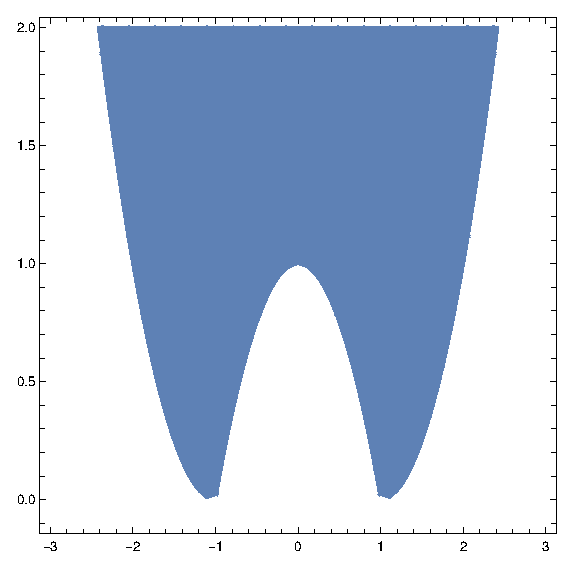
\includegraphics[width=\textwidth]{Chapter2/media/K1.eps}
         \caption{$K_1$}
        \label{fig.pwl.K1}
 \end{subfigure}
  \hfill
 \begin{subfigure}[b]{0.19\textwidth}
         \centering
         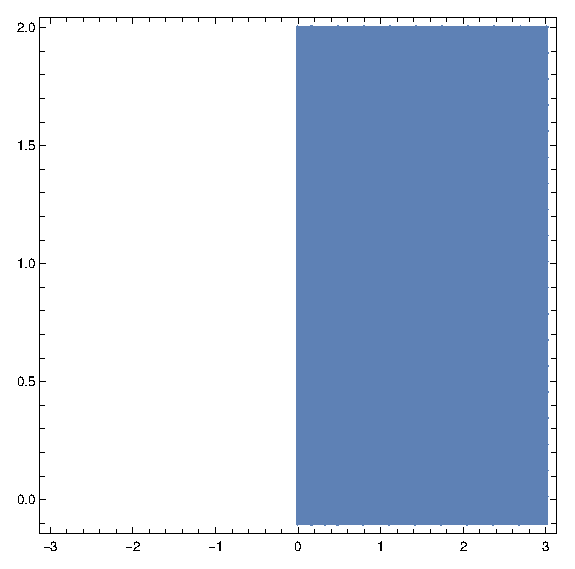
\includegraphics[width=\textwidth]{Chapter2/media/K2.eps}
         \caption{$K_2$}
        \label{fig.pwl.K2}
 \end{subfigure}
  \hfill
  \begin{subfigure}[b]{0.19\textwidth}
         \centering
         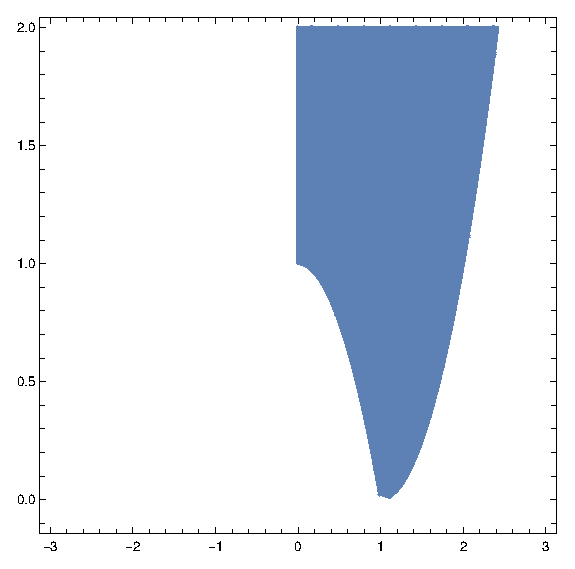
\includegraphics[width=\textwidth]{Chapter2/media/K.eps}
         \caption{$K$}
        \label{fig.pwl.K}
 \end{subfigure}
  \hfill
  \begin{subfigure}[b]{0.19\textwidth}
         \centering
         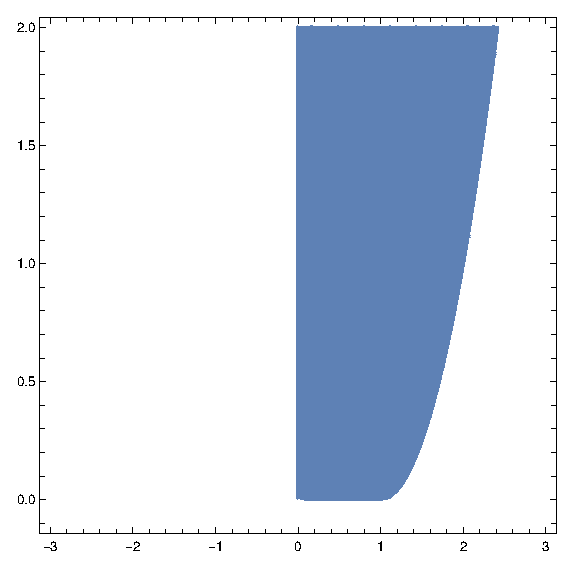
\includegraphics[width=\textwidth]{Chapter2/media/Khull.eps}
         \caption{$\conv(K_1) \cap K_2$}
        \label{fig.pwl.Khull}
 \end{subfigure}
  \hfill
   \begin{subfigure}[b]{0.19\textwidth}
         \centering
         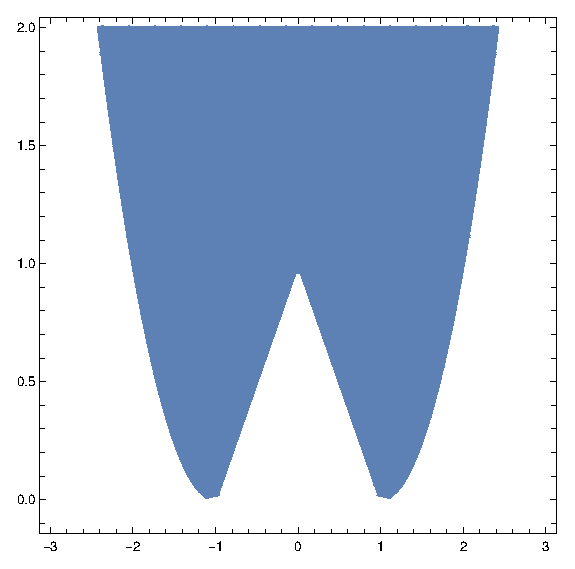
\includegraphics[width=\textwidth]{Chapter2/media/Kpwl.eps}
         \caption{$\bar{K}_1$}
        \label{fig.pwl.Kpwl}
 \end{subfigure}
  \caption{PWL approximation of nonconvex sets.}
  \label{fig.pwl}
\end{figure}




\section{Relaxation tightening via intersection cuts}
\label{sec.premic}
The cutting plane algorithm aims to construct a polyhedral outer approximation $P$ of the nonconvex set $\cS$, which is the feasible set of the MINLP problem $\min_{x \in \cS} c x$. Thereby, the polyhedron $P$ yields an LP relaxation of the MINLP problem.  Intersection cuts are a particular type of  valid inequalities that can tighten the polyhedral outer approximation.


The construction of intersection cuts \cite{conforti2014} requires two key ingredients: a simplicial cone containing  $\cS$, and an $\cS$-free set, which is defined as follows.

\begin{definition}
    \label{def.free}
    Given  a set $\cS \subsetneq \bR^p$, a closed set $\cC$ is (convex) $\cS$-free if $\cC$ is convex and $\inter(\cC) \cap \cS = \varnothing$.
    \end{definition}

Thinking reversely, $\cS$-free sets are convex regions whose  interiors have no element of $\cS$, so $\cS$-free sets can describe ``non-feasible'' regions of a MINLP problem.



\Cref{fig.sdef} shows an example of a $\cS$-free set, where we find  that  $\cC$ is a convex inner approximation of  $\cl(\cS^c)$.


Intersection cuts were initially devised in the continuous setting (the papers \cite{tuy64}, cited in \cite[Ch.~III]{horsttuy}, appeared before the classic paper \cite{balas1971intersection}), where they could approximate the hypograph $\cS$ of a convex function over a polytope.   There is a  unique  maximal  $\cS$-free set: the epigraph  of that convex function. Later, intersection cuts were used in the discrete setting \cite{balas1971intersection}, where $\cS$ is  a lattice. Several more families of lattice-free sets ({\eg}~splits, triangles, and spheres \cite{conforti2014,liberti2008spherical}) were described later.

We show how to construct $\cS$-free sets from a ``reverse'' representation of some nonconvex sets. We  look at  sets involving a particular type of nonconvex functions.

\begin{definition}
A function $f$ is said to be  difference-of-concave (DCC), if  there exists two concave functions $f_1,f_2$ such that $f=f_1 - f_2$.
\end{definition}

It is easy to show that the negative of a DCC function is also a DDC function, and thus any DC function is also a DCC function. A nonconvex set admits a \emph{DCC formulation}, if it is represented as the sublevel set of a DCC function. We call such a set \emph{a DCC set}.  The superlevel set of a DCC function is a sublevel set of another DDC function (the negative of that function), so one can reformulate the superlevel set into a DCC set.  For a  function $f$ and a point $\relx{x}$ in its domain, we denote the first-order approxiamtion $f(\relx{x}) + \nabla f(\relx{x})(x - \relx{x})$ of $f$ as $\lin{f}{\relx{x}}(x)$. The following  lemma gives a family of $\cS$-free sets for DCC sets via \emph{linearization method}.

\begin{lemma}[\cite{serrano2019}]\label{cor.dc2} 
Let $\cS := \{x \in \bR^p: f_1(x) - f_2(x) \le 0\}$, where  $f_1, f_2$ are concave functions over $\bR^p$. Then  for any $\relx{x} \in \bR^p$, $\cC := \{x \in \bR^p: f_1(x) - \lin{f_2}{\relx{x}}(x) \ge 0\}$ is $\cS$-free. Moreover, if $\relx{x} \in \bR^p \smallsetminus \cS$, $\relx{x} \in \inter(\cC)$.
\end{lemma}

To apply the above lemma, it suffices to reverse the inequality defining  $\cS$ and linearize its convex part. We refer to $\relx{x}$ as a \emph{linearization point} of $f_2$. Note that when the common domain  $\cG$ of $f_1$ and $f_2$ is not $\bR^p$,  $\cS$ should be restricted to the \emph{ground set} $\cG$.


\begin{figure}
 \centering
  \subfloat[$\cC$ as an $\cS$-free set.]{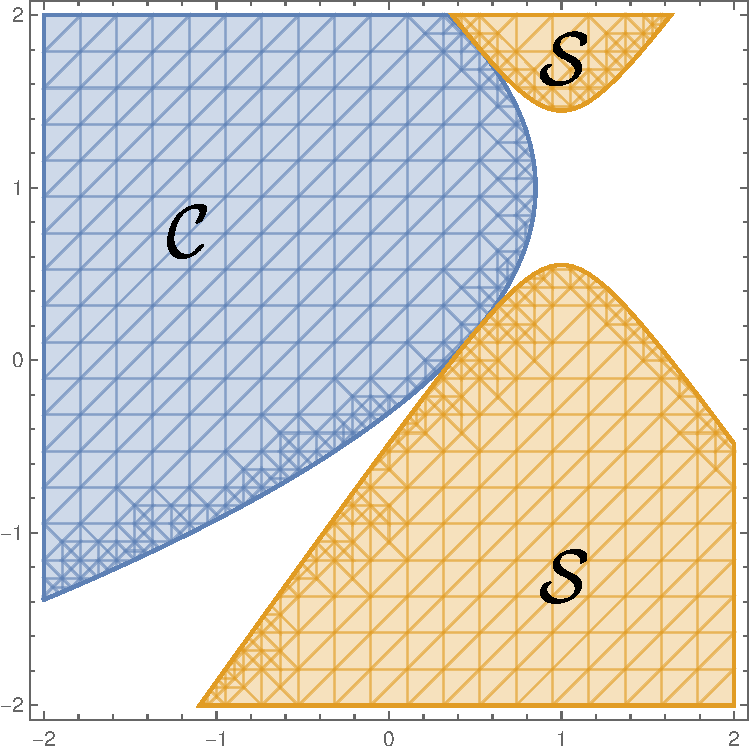
\includegraphics[width=0.3\textwidth]{Chapter2/media/sdef.pdf}}
  \hfill
  \subfloat[$\cC$ as an inner approximation of $\cl(\cS^c)$.]{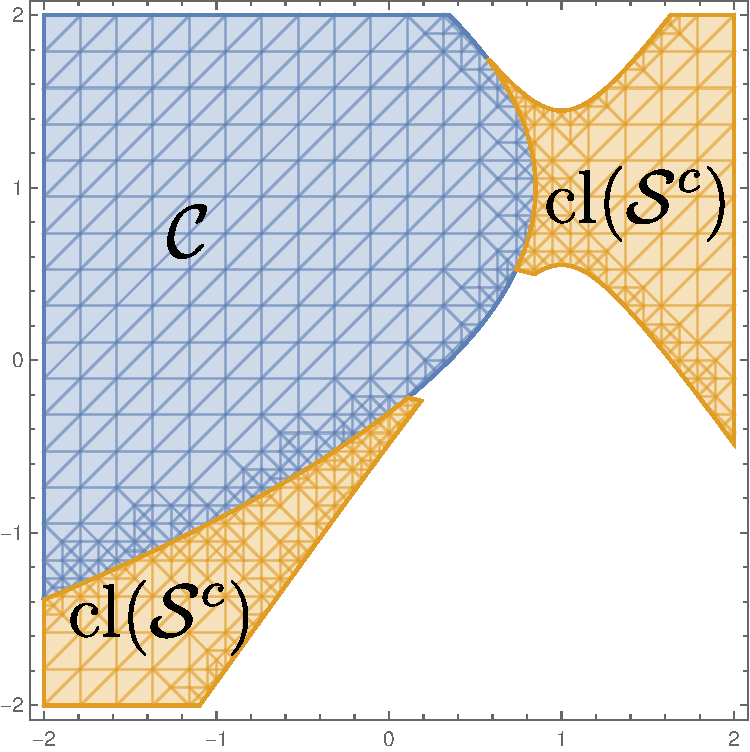
\includegraphics[width=0.3\textwidth]{Chapter2/media/sfreeinner.pdf}}
  \caption{An $\cS$-free set $\cC$.}
  \label{fig.sdef2}
\end{figure}
We show some examples in \Cref{fig.sdef2}.

Given an $\cS$-free set, the next step is to construct an intersection cut. The construction procedure requires additionally a translated polyhedral cone $\cR$  such that $\cS \subseteq \cR$ and the vertex $\relx{x}$  of $\cR$ is not in $\cS$. Let us suppose that $\cR$ admits a hyper-plane representation: $
     \{x \in \bR^p: B(x - \relx{x}) \le 0\}, $
where $B$ is a $p \times p$ invertible matrix. For all $j\in[p]$, let $r^j$ denote the $j$-th column of $-B^{-1}$, then $r^j$ turns out to be an extreme ray of $\cR$. Thereby, $\cR$ also admits a ray representation $
   \{x \in \bR^p:\exists \eta \in \bR^p_+ \textup{ }  x =\relx{x} +  \sum_{j =1}^{p} \eta_jr^j \}, $

    
For all $j \in [p]$, we define the \textit{step length} from $\relx{x}$ along ray $r_j$ to the boundary  $\bd(\cC)$ as
\begin{equation}
 \label{eq.iccoef}
   \eta_j^\ast := \max_{\eta_j \in [0,+\infty]}\{\eta_j: \relx{x} + \eta_j r^j \in \cC\}.
\end{equation}
Then, the intersection cut admits the form:
\begin{equation}
 \label{eq.ic}
     \sum_{j =1}^{p} \frac{1}{\eta_j^\ast} B_j (x - \relx{x}) \le -1,
 \end{equation}
where $B_j$ is the $j$-th row of $B$. When all step lengths are positive, the above linear inequality cuts off $\relx{x}$ from $\cS$.   The construction of an intersection cut is visualized in \Cref{fig.sdef}.

\begin{figure}
    \centering
     \subfloat[$\cC$ as an inner approximation of $\cl(\cS^c)$.]{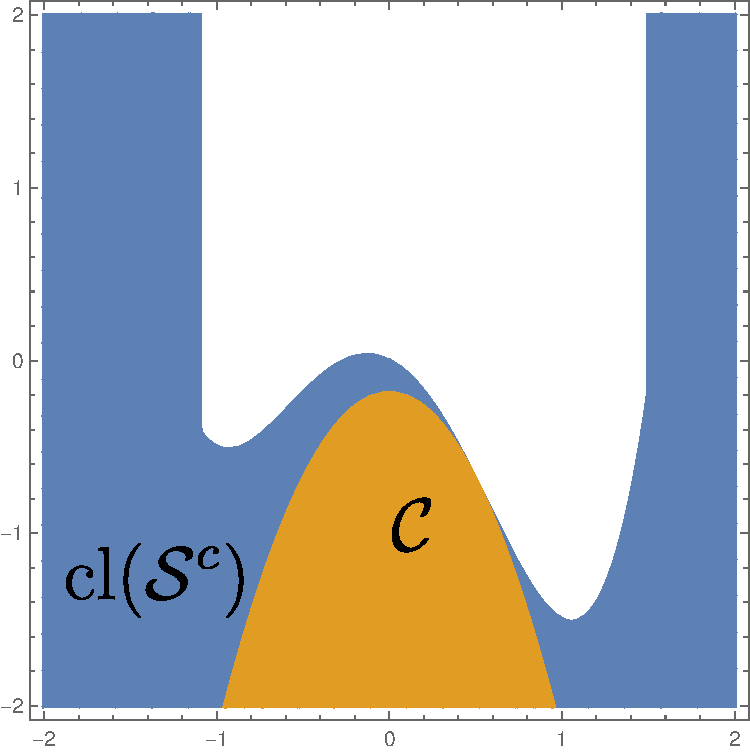
\includegraphics[width=0.3\textwidth]{Chapter2/media/s11.pdf}}
     \hfill
     \subfloat[$\cC$ as an $\cS$-free set.]{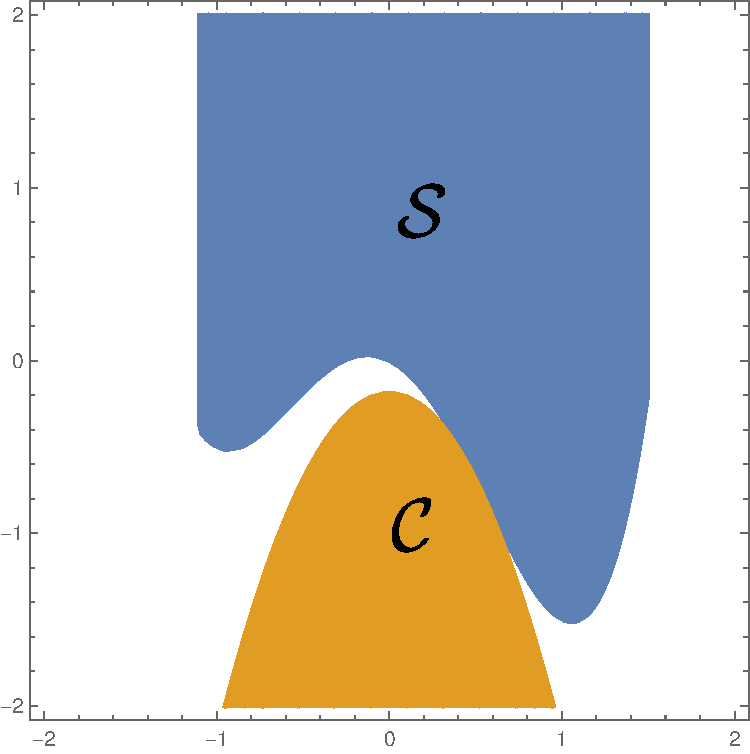
\includegraphics[width=0.3\textwidth]{Chapter2/media/s12.pdf}}
     \hfill
   \subfloat[Simplicial cone $\cR$ and the intersection cut.]{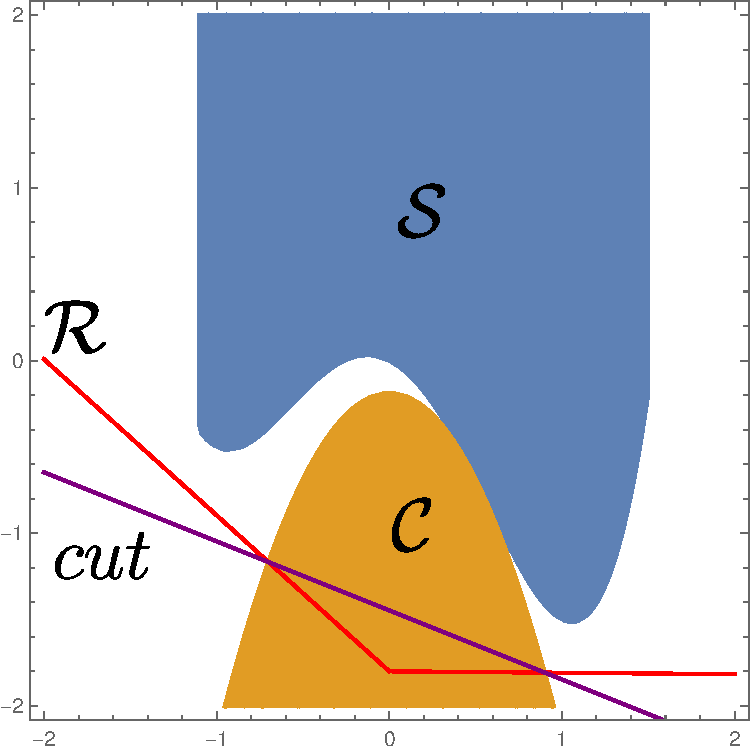
\includegraphics[width=0.3\textwidth]{Chapter2/media/s13.pdf}}
     \caption{An $\cS$-free set $\cC$, simplicial cone $\cR$, and intersection cut.}
     \label{fig.sdef}
   \end{figure}

In practice, we can obtain $\cS$, $\cR$, and $\relx{x}$  as follows. Assume that we have an LP relaxation $\min_{x \in \cP} c x$ of the MINLP problem, where $\cP$ is a polyhedral outer approximation of the feasible set. If the LP solution is not feasible to SP, as the LP relaxation usually comprises all linear constraints of the MINLP problem, then the solution must not satisfy some  nonlinear constraint.  Thus, we can set $\relx{x}$ to the LP solution and define $\cS$ by  the nonlinear constraint. Moreover,  we can extract $\cR$ from the basis of the LP defining $\relx{x}$. 


The main issue we address is therefore the construction of  (maximal) $\cS$-free sets.  The reason why we look for \emph{maximal} such sets is that, if
$\cC$ and $\cC^\ast$ are two $\cS$-free sets with $\cC \subseteq \cC^\ast$, then the intersection cut derived from $\cC^\ast$ dominates the intersection cut derived from $\cC$. Thereby, we give a formal definition of maximal $\cS$-free sets.

\begin{definition}
\label{def.max}
Given  a closed convex set $\cG \subseteq \bR^p$ such that $\cS \subsetneq \cG$, an  $\cS$-free set $\cC$ is (inclusion-wise) maximal in $\cG$,  if there is no other $\cS$-free set $\cC'$ such that $\cC \cap \cG \subsetneq \cC' \cap \cG $.
\end{definition}

\Cref{def.max} generalizes the conventional definition of  maximal $\cS$-free sets, and one can recover the conventional definition by setting $\cG = \bR^p$.  In some cases, it is difficult to study the maximality of $\cS$-free sets in $\bR^p$. \Cref{def.max} allows us to study intersections of $\cS$-free sets with the \emph{ground set}  $\cG$.  


\section{Conclusion}

In this section, we present a class of common relaxation methods. In the next chapter, we introduce some advanced theoretical results for relaxing structured sets. They yield new relaxation methods. In the rest of the thesis, we apply these methods to tackle applications that can be modelled as MINLP problems.

\chapter{Theory: advanced structural results}
\label{chap.theorystructure}



Within this chapter, we introduce innovative theoretical findings related to the process of convexification or relaxation of structured sets. These findings have been developed to address practical challenges encountered throughout this thesis and will serve as the foundation for the development of cutting-edge algorithms for various problems. These results can be regarded as advanced concepts building upon the submodularity and intersection cut framework introduced in \Cref{chap.basic}.

\section{$\cS$-free sets for structured sets}
\label{sec.advanced}

In this section, we introduce advanced results concerning the intersection cut framework. We have demonstrated that the intersection cuts relies on the concept of $\cS$-free sets, which in turn, depend on the specific problem structure. The set $\cS$ under consideration encompasses sets originating from NLP and those arising in submodular optimization.


\subsection{Maximal $\cS$-free sets for lifted sets}
\label{sec.lift}
We  consider  the extended formulation \eqref{minlp3} of a general NLP problem and focus on the associated lifted set $\cSl$ in \eqref{eq.lift}.  We show a lifting result on the construction of maximal $\cSl$-free sets.



Let $z\deq(x,y)$ denote the vector variable in the extended formulation \eqref{minlp3}, with its index set being $[n+k]$. Consequently, we have $z_{[n]} = x$ and $z_{[n+1:n+k]} = y$. Consider a closed subset $\cX$ of the domain $\bigcap_{i \in [k]} \dom(g_i)$ for $x$, and let $\cY$ be a closed subset of the domain $\bigtimes_{i \in [k]} \rang(g_i)$ for $y$. The ground set $\cG$, where the variables actually vary, can be set as $\cX \times \cY$. Consequently, the lifted set $\cSl$ in \eqref{eq.lift} admits the form $\{(x,y) \in \cG: y = g(x)\}$.

Given that each $g_i(x)$ (for $i\in[k]$) may only depend on a subset of  variables indexed by $J_i \subseteq [n]$, we can express $g_i(x)$ as a lower order function $g'_i(x_{J_i})$ defined over $\bR^{|J_i|}$. Let $I_i \deq J_i \cup \{i + n\}$. As above, we consider a closed subset $\cX^i$ of $\dom(g'_i)$ and $\cY^i$ of $\rang(g'_i)$. Consequently, the graph, epigraph, and hypograph of $g'_i$ reside within sets $\cG^i \deq \cX^i \times \cY^i$, \eg $\epi(g'_i)=\{(x_{J_i}, y_i) \in \cG^i: g'_i(x_{J_i}) \le y_i\}$.

We refer to $\cX,\cY, \{\cX^i, \cY^i\}_{i \in [k]}$ as the \emph{underlying sets} of the lifted set $\cSl$. The sets are said to be \emph{1d-convex decomposable} by a collection $\{\cD_j \}_{j \in [n+k]}$ of closed  convex sets in $\bR$, if  $\cX= \bigtimes_{j \in [n]}\cD_j, \cY= \bigtimes_{j \in [n+1:n+k]}\cD_j$, and, for all $i \in [k]$, $\cX^i = \bigtimes_{j \in J_i}\cD_j, \cY^i = \cD_{n+i}$. This decomposability condition restricts the domains to Cartesian products of real lines, intervals, or half rays, thereby excluding complicated domain structures.

The decomposability condition allows for the analysis of sets involving fewer variables. Constructing $\epi(g'_i)$-free sets and $\hyp(g'_i)$-free sets is generally easier than constructing $\cSl$-free sets.  We show that every maximal $\epi(g'_i)$-free or $\hyp(g'_i)$-free set can be lifted into a  maximal $\cSl$-free set.

\begin{theorem}
\label{thm.decomp}
Suppose the underlying sets of $\cSl$ are 1d-convex decomposable and $g$ is continuous. For some $i \in [k]$, let $\cC$ be a maximal $\epi(g'_i)$-free set or a maximal $\hyp(g'_i)$-free set in $\cG^i$. Then $\bar{\cC}\deq \cC \times \bR^{|I^c_i|}$ ($I^c_i = [n+k] \setminus I_i$) is a maximal $\cSl$-free set in $\cG$.
\end{theorem}
\begin{proof}
It suffices to consider the case that $\cC$ is a maximal $\epi(g'_i)$-free set in $\cG^i$. W.l.o.g., we can assume that $\cC,  \cG^i$ are full-dimensional in $\bR^{|I_i|}$. Since $\epi(g'_i)$ includes $\gr(g'_i)$, $\cC$, as an $\epi(g'_i)$-free set,  is also $\gr(g'_i)$-free. First, we prove that  $\cC$ is a maximal $\gr(g'_i)$-free set in $\cG^i$. Assume, to aim at a contradiction, that $\cC'$ is a $\gr(g'_i)$-free set that $\cC \cap \cG^i \subsetneq \cC' \cap \cG^i$.  Suppose that $\epi(g'_i)  \cap \inter(\cC' \cap \cG^i)$ is not empty and contains $(x'_{J_i}, y'_i)$.     As $\cC$ is  $\epi(g'_i)$-free, there exists a point $(x_{J_i}, y_i) \in \inter(\cC \cap \cG^i) \subseteq \inter(\cC' \cap \cG^i)$ such that $(x_{J_i}, y_i) \in \hyp(g'_i)$.  It follows from the continuity of $g'_i$  that there exists a point $(x^\ast_{J_i}, y^\ast_i) \in \gr(g'_i)$ in the line segment joining $(x_{J_i}, y_i)$ and $(x'_{J_i}, y'_i) $. As $\inter(\cC' \cap \cG^i)$ is convex,  we have that $(x^\ast_{J_i}, y^\ast_i) \in \inter(\cC' \cap \cG^i)$, which leads to a contradiction to $\gr(g'_i)$-freeness of $\cC'$. Therefore, $\epi(g'_i)  \cap \inter(\cC' \cap \cG^i)$ must be empty, so $\cC' \cap \cG^i  \subseteq \hyp(g'_i)$. This means that $\cC'$ is also $\epi(g'_i)$-free. However, note that  $\cC \cap \cG^i \subsetneq \cC' \cap \cG^i$, this contradicts with the fact that $\cC$ is a maximal $\epi(g'_i)$-free set in $\cG^i$. Therefore, $\cC$  is a maximal $\gr(g'_i)$-free set in $\cG^i$. Secondly, we  prove that $\bar{\cC}$ is a maximal $\cSl$-free set in $\cG$.
Assume, to aim at a contradiction, that there exists an $\cSl$-free set $\bar{\cD}$ in $\cG$ such that $ \bar{\cC} \cap \cG \subsetneq \bar{\cD} \cap \cG$. We look at their orthogonal projections on  $\bR^{|I_i|}$. It follows from the decomposability  that $\cC \cap \cG^i = \cC \cap \proj_{\bR^{|I_i|}} (\cG) = \proj_{\bR^{|I_i|}}(\bar{\cC} \cap \cG) \subseteq \proj_{\bR^{|I_i|}}(\bar{\cD} \cap \cG)$. Denote $\cD \deq \cl(\proj_{\bR^{|I_i|}}(\bar{\cD} \cap \cG))$, which is a closed convex set in $\cG^i$. Since $\bar{\cC}= \cC \times \bR^{|I^c_i|}$, $\cD$  must strictly include $\cC \cap \cG^i$. Note that $\cD$ is $\gr(g'_i)$-free. Since $\cC$ is a maximal $\gr(g'_i)$-free set in $\cG^i$, this implies that $\cC \cap \cG^i = \cD$, which leads to a contradiction.
\end{proof}

 For any $i\in[k]$, we call the operation $\cC \times \bR^{|I^c_i|}$ the \emph{orthogonal lifting} of $\cC$ w.r.t. $g_i$. A similar lifting result for integer programming is provided by Lemma 4.1 of \cite{conforti2011}: given $\cS \deq \bZ^{n} \times \bR^{h}$, any maximal lattice-free set (\ie $\bZ^n$-free set) can be transformed into a maximal $\cS$-free set through orthogonal lifting. Therefore, \Cref{thm.decomp} serves as the NLP counterpart to that lemma (whose proof is also similar). This theorem allows us to focus on low-dimensional projections of the lifted set.

 We will show in \Cref{cor.maxsig} that the signomial lift satisfies the prerequisites of  \Cref{thm.decomp}.
The following example illustrates the application of \Cref{thm.decomp}.

\begin{example}
 Consider a lifted set $\cSl$ defined as $$\{(x_1,x_2,x_3,x_4, y_1,y_2, y_3): y_1= \exp(x_1 - x_2 /x_3),  y_2 = \log(x_1), y_3 = \sin(x_1 / x_4)\}.$$

One can verify that the 1d-convex decomposable condition holds for $\cD_1 = \bR_+$,  $\cD_j = \bR$ (for $j \in [2:7]$). Then $\cG\deq \bR^1_+ \times \bR^6$.  We use $\log(x_1)$ to construct a $\cSl$-free set. A maximal $\cSl$-free set can be $\{(x_1,x_2,x_3,x_4, y_1,y_2, y_3) \in \cG:  y_2 \le \log(x_1)\}$. Since $\log(x_1)$ is defined over positive  reals, this example gives a reason to restrict maximality over $\cG$.
\end{example}




\subsection{Maximal $\cS$-free for DCC constraints}

We provide sufficient conditions for the maximality of $\cS$-free sets for two general classes of non-convex sets $\cS$. To begin with, we review some fundamental results from convex analysis. Our subsequent presentation relies on the use of support functions of convex sets. The properties of support functions can be summarized as follows.


\begin{lemma}[Chapter C of \cite{hiriart2004fundamentals}]
\label{lem.supconv}
 For  a full-dimensional closed convex set  \(\cC \subsetneq \bR^p\), let \(\sigma_{\cC}: \bR^p \to \bR, \lambda \mapsto \sup_{z \in \cC}{\lambda}\cdot z\) be the support function of \(\cC\). Then: (i) \label{lem.supconv2} \(\cC = \{z \in \bR^p: {\lambda}\cdot z\le \sigma_{\cC}({\lambda}), \forall {\lambda} \in \dom(\sigma_{\cC}) \}\), (ii)  \(\inter(\cC) = \{z \in \bR^p:{\lambda}\cdot z <\sigma_{\cC}({\lambda}),  \forall {\lambda} \in  \dom(\sigma_{\cC})  \smallsetminus\{0\} \}\), (iii)
	$\sigma_{\cC}(\rho \lambda) = \rho \sigma_{\cC}(\lambda)$ for any $\rho > 0$. Moreover, for any closed convex set \(\cC'\) including $\cC$,   $\sigma_{\cC} \le \sigma_{\cC'}$.
\end{lemma}

 A valid inequality $a \cdot z \le b$ of $\cC$ is  called a \emph{supported valid inequality}, if there exists a \emph{supporting point} $z' \in \bd(C)$ such that \(a \cdot z' =  b\).  Geometrically, a closed convex set is the intersection of half-spaces associated with supported valid inequalities.


 \begin{observation}
  It follows from \Cref{lem.supconv} that every supported valid inequality of $\cC$ must admit the form $\lambda \cdot z\le \sigma_{\cC}(\lambda)$  for some $\lambda \in \dom(\sigma_{\cC})$, where the supremum  $\sigma_{\cC}(\lambda)$ is attained at its supporting points.
 \end{observation}

An inequality of the form $\lambda \cdot z \leq \sigma_{\cC}(\lambda)$, for $\lambda \in \dom(\sigma_{\cC})$, is referred to as an \emph{exposed valid inequality}, if there exists an \emph{exposing point} $z' \in \bd(C)$ such that $\lambda \cdot z' = \sigma_{\cC}(\lambda)$ and  for all \({\lambda'} \in \dom(\sigma_\cC) \smallsetminus\{{\rho\lambda}\}_{\rho > 0}\), \({\lambda'}\cdot z' < \sigma_{\cC}(\lambda')\).
 
  \begin{observation}
  \label{obs.1}
An exposed valid inequality must be a supported valid inequality. Conversely, a supported valid inequality  is  an exposed valid inequality, if manifold $\bd(\cC)$ is smooth at its supporting point.  For example, $\cC_1\deq\{(x,y) \in \bR^2: y = x^2\}$ is a smooth manifold, so every supported valid inequality of $\cC_1$ is exposed; $\cC_2\deq\{(x,y) \in \bR^2: y = |x|\}$ is smooth at $x \in [1,2]$, so every supported valid inequality of $\cC_2$ with supporting point $(x,y)$ ($x \in [1,2]$)  is  also exposed by the same point; however,  a supported valid inequality of $\cC_2$ with supporting point $(x,y)$ ($x = 0$)  cannot be exposed, since there are infinitely many  supported valid inequalities at the same point.
 \end{observation}
 

The first theorem we present applies to full-dimensional nonconvex sets $\cS$. We observed the geometric equivalence between the closed convex inner approximation of $\cl(\cS^c)$ and $\cS$-free sets. The theorem provides a sufficient condition for the maximality of closed convex inner approximations.


\begin{theorem}\label{prop.max}
	Let \(\cF\) be a full-dimensional closed set in \(\bR^p\), and let \(\cC  \subseteq  \cF\) be a full-dimensional closed convex set. If, for any \(z^\ast \in \inter(\cF \smallsetminus \cC)\) and any  $\lambda \in \dom(\sigma_{\cC})$ such that $\lambda \cdot z^\ast > \sigma_{\cC}(\lambda)$, there exists a point $z' \in \bd(\cF) \cap \bd(\cC)$ exposing $\lambda \cdot z \le \sigma_{\cC}(\lambda)$, then $\cC$ is a maximal convex inner approximation of $\cF$.
	\end{theorem}
	\begin{proof}
 Let $\cC$ be a set satisfying the hypothesis.  Suppose, to aim at a contradiction, that there exists a closed convex set $\cC^\ast$ such that $\cC \subsetneq \cC^\ast$  and $\cC^\ast$ is an inner approximation of $\cF$. Then, there must exist  an open ball $B$ such that  \( B \subseteq \cF \smallsetminus\cC\) and $B \subseteq  \cC^\ast$. Let $z^\ast$ be the center of $B$, so   $z^\ast \in  \inter(\cF \smallsetminus \cC)$. W.l.o.g., we let $\cC^\ast = \conv(\cC \cup \{z^\ast\})$, which is a closed convex inner approximation of $\cF$. Since $z^\ast \notin \cC$, by the hyperplane separation theorem, there exists  \({\lambda} \in \dom(\sigma_{\cC})\) such that
	\begin{equation}
    	\label{eq.r0}
	{\lambda}\cdot z^\ast > \sigma_{\cC}({\lambda}).
	\end{equation}
	For any such $\lambda$, by the hypothesis, there exists a point \(z' \in \bd(\cF) \cap \bd(\cC)\) such that
	\begin{equation}
	\label{eq.r1}
  	{\lambda} \cdot z'  = \sigma_{\cC}({\lambda}),  
	\end{equation}
	and $z'$ is an exposing point of $\cC$. We want to show that,  for any \({\lambda'} \in \dom(\sigma_{\cC^\ast})\), \({\lambda'}\cdot z' < 	\sigma_{\cC^\ast}({\lambda})\). We consider the following three cases. First, we consider the case $\lambda'=\lambda$.  Because \(z^\ast \in \cC^\ast\), by the definition of support functions, we have that
 	\begin{equation}
     	\label{eq.r2}
     	{\lambda} \cdot z^\ast \le \sup_{z \in \cC^\ast}{\lambda}\cdot z = \sigma_{\cC^\ast}({\lambda}).
 	\end{equation}
	It follows from \eqref{eq.r0}, \eqref{eq.r1}, and \eqref{eq.r2} that
	\begin{align}
	\label{eq.r4}
    	{\lambda} \cdot z'  =  \sigma_{\cC}({\lambda}) < {\lambda} \cdot z^\ast \le \sigma_{\cC^\ast}({\lambda}) = \sigma_{\cC^\ast}({\lambda'}).
	\end{align} Second, we consider the case $\lambda ' = \rho \lambda$ for some $\rho > 0$. Since $\sigma_{\cC^\ast}$ is positively homogeneous of degree 1, it follows from \eqref{eq.r4} that $\lambda' \cdot z' =  {\rho \lambda} \cdot z' < \rho \sigma_{\cC^\ast}({ \lambda}) = \sigma_{\cC^\ast}({\lambda'}).$ Last, we consider the case ${\lambda'} \in \dom(\sigma_{\cC^\ast}) \smallsetminus\{{\rho \lambda}\}_{\rho > 0}$. By \Cref{lem.supconv}, $\sigma_{\cC} \le \sigma_{\cC^\ast}$. 
	By the hypothesis that $z'$ is an exposing point of $\cC$, provided that $\lambda' \ne \rho \lambda$,  we have that
	$
    	{\lambda'}\cdot z' < \sigma_{\cC}({\lambda'}) \le	\sigma_{\cC^\ast}({\lambda'}).
	$
	In summary, we have proved that, for any \({\lambda'} \in \dom(\sigma_{\cC^\ast})\), \({\lambda'}\cdot z' < 	\sigma_{\cC^\ast}({\lambda'})\). So by \Cref{lem.supconv}, \(z' \in \inter(\cC^\ast)\). We find that $z' \in \bd(\cF) \cap \inter(\cC^\ast)$. This finding means a point near  $z'$ exists, which is in $\cC^\ast$, but not in $\cF$. Hence, $\cC^\ast$ is not an inner approximation of $\cF$, which leads to a contradiction.
	\end{proof}
 
%% LEO 230719: I think this paragraph should replace the two paragraphs below, which I found confusing.
We call  $z^\ast$ in \Cref{prop.max} an \emph{outlier point}, by which we try to enlarge an $\cS$-free set, and let $L(z^\ast):=\{\lambda \in \dom(\sigma_{\cC}):\lambda \cdot z^\ast > \sigma_{\cC}(\lambda)\}$. The proof of Thm.~\ref{prop.max} was adapted from that of \cite[Thm.~2]{munoz2020maximal}, which excludes the presence of the outlier point and requires a stronger assumption, namely that, for any $\lambda \in \dom(\sigma_{\cC})$ there exists a point $z' \in \bd(\cF) \cap \bd(\cC)$ exposing $\lambda \cdot z \le \sigma_{\cC}(\lambda)$. As we will see in the proof of \Cref{thm.max}, $\bigcup_{z^\ast \in \inter(\cF \smallsetminus \cC)} L(z^\ast)$ can be a proper subset of $\dom(\sigma_{\cC})$, so we do not need to check that all $\lambda \in \dom(\sigma_{\cC})$ are exposed.
 

We next focus on a specific type of function, namely  \emph{positive homogeneous functions}.  We summarize their properties as follows.
\begin{lemma}
	\label{lem.homo}
Let  $f$  be a positive homogeneous function of degree $d \in \bR$, such that  for any $z \in \dom(f) \subseteq \bR^p$ and any $\rho \in \bR_{++}$, $f(\rho z)=\rho^d f(z)$. Then: (i) $\inter(\dom(f))$ is a cone, and (ii) if $d=1$, Then, for any $\breve{z} \in \dom(f)$, \(\lin{f}{\breve{z}}(z) =\nabla  {f}(\breve{z})\cdot z\) for $z \in \dom(f)$ and \(\lin{f}{\breve{z}}(z)  = f(z)\) for \( z = \rho \breve{z}\) with \(\rho \in \bR_{++}\).
\end{lemma}
\begin{proof}
Given $z \in \dom(f)$, $f(\rho z)= \rho^d f(z) $ is a real number for any  $\rho \in \bR_{++}$, so $\inter(\dom(f))$ is a cone.
Suppose that $f$ is positive homogeneous of degree 1. For any $z \in \dom(f)$,
$
	\lin{f}{\breve{z}}(z) = f(\breve{z}) + \nabla  {f}(\breve{z}) \cdot (z - \breve{z}) =  \nabla  {f}(\breve{z}) \cdot z,
$
where  the second equation follows from Euler's homogeneous function theorem: $f(\breve{z}) = \nabla {f}(\breve{z}) \cdot \breve{z}$. For any \( z = \rho \breve{z}\) with \(\rho \in \bR_{++}\),
$
	\lin{f}{\breve{z}}(z)  = \nabla  {f}(\breve{z})\cdot \rho \breve{z} = \rho  \lin{f}{\breve{z}}(\breve{z}) =\rho f( \breve{z}) = f(\rho \breve{z}),
$
where the first and second equations follow from the previous result, the third follows from that $\lin{f}{\breve{z}}$ has the same value as $f$ at $\breve{z}$, and the last equation follows from the homogeneity.
\end{proof}

We recall that $\lin{f}{\breve{z}}$ in the above lemma is the first order linearization of $f$ at $\breve{z}$. Moreover, $\dom(f)$ is embedded in $\bR^p$, so we call $\bR^p$ the \emph{ambient space} of $f$.


The second theorem we present offers a more structured result specifically addressing nonconvex DCC sets $\cS$. \cite[Thm.~5.48]{serranothesis} provides a sufficient condition for the maximality of the $\cS$-free set described in \Cref{cor.dc2}. However, to clearly differentiate it from our subsequent result, we translate the condition into our setting as follows: (i) the functions $f_1$ and $f_2$ are superlinear, meaning they are positive homogeneous of degree 1 and super-additive (note that superlinear functions are concave), (ii) they are separable and act independently on different variables $u$ and $v$, (iii) $f_1$ is negative everywhere except at 0, (iv) the linearization point $\relx{v}$ of $f_2$ is nonzero, and (v) the domains $\dom(f_1)$ and $\dom(f_2)$ are Euclidean spaces.

Our second theorem provides an alternative condition for maximality that relaxes the condition (i) by requiring only one of $f_1$ or $f_2$ to be positive homogeneous of degree 1, while imposing mild regularity conditions. Additionally, it allows the domains to be  full-dimensional convex cones.

\begin{theorem}
\label{thm.max}
	For every $i \in \{1,2\}$, let  $f_i$ be   concave.  Let $\cS \deq \{(u,v) \in \dom(f_1) \times \dom(f_2): f_1(u) - f_2(v) \le 0\}$. Suppose that: (i) at least one  of $f_1,f_2$ is positive homogeneous of degree 1, (ii) $f_1,f_2$ are both positive/negative over the interiors of their domains, (iii) $f_1$ is continuously differentiable over $\inter(\dom(f_1))$, and  (iv) $\dom(f_1),\dom(f_2)$ are full-dimensional in the ambient spaces of $f_1,f_2$, respectively. Then, for any $\relx{v} \in \inter(\dom(f_2))$, $\cC \deq \{(u,v) \in \dom(f_1) \times \dom(f_2): f_1(u) -\lin{f_2}{\relx{v}}(v) \ge 0\}$ is maximally $\cS$-free in $\dom(f_1) \times \dom(f_2)$.    
\end{theorem}
\begin{proof}
	We first adapt \Cref{cor.dc2} by restricting the domain of $z$ to the convex ground set $\cG\deq\dom(f_1) \times \dom(f_2)$. It follows from \Cref{cor.dc2} that $\cC$ is  an $\cS$-free set in $\cG$. Since $\dom(f_1) \times \dom(f_2)$ are full-dimensional, $\cS,\cC, \cG$ are  full-dimensional. As $\cS,\cC \subseteq \cG$, the maximality of $\cC$ in $\cG$ is equivalent to that $\cC$ is a maximal convex inner approximation of $\cF\deq\cl(\cS^c) \cap \cG = \{(u,v) \in \cG: f_1(u) -f_2(v) \ge 0\}$. Note that $\cF$ is  full-dimensional. We then apply \Cref{prop.max} to prove that $\cC$ is a maximal convex inner approximation of $\cF$.  Let \(z^\ast \in \inter(\cF \smallsetminus \cC)\) be any outlier point. It follows from the separating hyperplane theorem that there exists a supported valid inequality $\lambda \cdot z \le \sigma_{\cC}(\lambda)$  of $\cC$ such that $\lambda \cdot z^\ast > \sigma_{\cC}(\lambda)$. Since $\cF \smallsetminus \cC \subseteq \cG$, $ \inter(\cF \smallsetminus \cC) \subseteq \cG$. Since $\cC \subseteq \cG$, the inequality cannot be supported by a valid inequality at $\bd(\cG)$, so the inequality must be a valid inequality supported at $\cC \smallsetminus \bd(\cG)$. It follows from the concavity of $f_1$ that the inequality must admit the form $\lin{f_1}{\breve{u}}(u) -\lin{f_2}{\relx{v}}(v) \ge 0$ for some $\breve{u} \in \dom(f_1)$ (identical up to a positive multiplier). By the smoothness of $f_1$, w.l.o.g, we can perturb $\breve{u}$ such that it is in $ \inter(\dom(f_1))$. Let $\breve{v} := \relx{v}$. We now have that $\breve{u} \in \inter(\dom(f_1)), \breve{v} \in \inter(\dom(f_2))$.  We will prove that $\lin{f_1}{\breve{u}}(u) -\lin{f_2}{\breve{v}}(v) \ge 0$ is exposed by a point $(u',v') \in (\bd(\cF) \cap \bd(\cC)) \cap \inter(\cG)$. It suffices to show that the following three equations hold:
	\begin{equation}
	\label{eq.three}
    	\begin{aligned}
        	\lin{f_1}{\breve{u}}(u') -\lin{f_2}{\breve{v}}(v') &= 0 \quad \textup{(\ie supported at $(u',v')$)},\\
        	f_1(u') -\lin{f_2}{\breve{v}}(v') &= 0  \quad \textup{(\ie $(u',v') \in \cC$)},\\
        	f_1(u') -f_2(v') &= 0 \quad  \textup{(\ie $(u',v') \in \cF$)}.
    	\end{aligned}
	\end{equation}
   Since $\cC \subseteq \cF$ and they  are both full-dimensional, the last two equations imply that $(u',v') \in \bd(\cC) \cap \bd(\cF)$. As $f_1$ is continuously differentiable and concave in the interior of its domain, the graph of $f_1(u) -\lin{f_2}{\breve{v}}(v)$  over $\inter(\cG)$ is a smooth manifold embedded in $\inter(\cG) \times \bR$. The intersection of a smooth manifold with a hyperplane yields another lower-dimensional smooth manifold. This implies that the  level set $\cC$ of $f_1(u) -\lin{f_2}{\breve{v}}(v)$ is also smooth at any point  $(u,v) \in \inter(\cG) \cap \cC$. By \Cref{obs.1}, $(u,v)$  is an exposing point.  Since $(u',v') \in \cC \cap  \inter(\cG)$, $(u',v')$ is an exposing point, and the maximality of $\cC$ is verified. We now proceed to construct $(u',v')$ from $(\breve{u},\breve{v})$ and prove \eqref{eq.three}.
  Let $\rho \deq  f_2(\breve{v}) / f_1(\breve{u})$.  Since $\breve{u} \in \inter(\dom(f_1)), \breve{v} \in \inter(\dom(f_2))$, by the assumption, $\rho  > 0 $.  We consider the following two cases separately.
  
  \textbf{Case i.} We first suppose that $f_1$ is positive homogeneous of degree 1.  Let $(u', v')\deq (\rho \breve{u}, \breve{v})$, which,  by \Cref{lem.homo}, is in $\inter(\cG)$.
We have that:
$$ 
  	f_1(u') \stackrel{(i.1)} = \lin{f_1}{\breve{u}}(u')
    	\stackrel{(i.2)}= \rho f_1(\breve{u})
    	\stackrel{(i.3)}= f_2(\breve{v})
    	\stackrel{(i.4)}= f_2(v') \stackrel{(i.5)}= \lin{f_2}{\breve{v}}(v'),
 $$ 
where equations $(i.1),(i.2)$ follow from \Cref{lem.homo},   $(i.3)$ follows from the definition of $\rho$, and $(i.4),(i.5)$  follow from $v'=\breve{v}$.
 
 \textbf{Case ii.}
We then suppose that $f_2$ is positive homogeneous of degree 1.  Let $(u', v')\deq ( \breve{u}, \breve{v} / \rho) \in \inter(\cG)$.
We have that:
$$
\lin{f_1}{\breve{u}}(u')   \stackrel{(ii.1)} =   f_1(u') \stackrel{(ii.2)} =  f_1(\breve{u})  
    	 \stackrel{(ii.3)} =  f_2(\breve{v}) /  \rho      	 \stackrel{(ii.4)} =   f_2(v') 
    	 \stackrel{(ii.5)} = \lin{f_2}{\breve{v}}(v'),
$$
	where equations $(ii.1), (ii.2)$ follow from $\breve{u} = u'$,  $(ii.3)$ follows from the definition of $\rho$, and  $(ii.4),(ii.5)$ follow  from \Cref{lem.homo}.  Therefore, \eqref{eq.three} are satisfied in both cases.
\end{proof}



We present the motivation for limiting the maximality of the set $\cC$ within the ground set $\dom(f_1) \times \dom(f_2)$. The primary reason for this restriction stems from the difficulty in finding a non-trivial concave extension of $f_1$ over its ambient space such that  for all $u \notin \dom(f_1)$, $f_1(u) > -\infty$. While such an extension may exist geometrically, the construction of a closed-form expression remains unclear. In the next section, we will examine a specific example to illustrate this point.

Furthermore, we will employ the aforementioned theorem to develop DCC formulations of a nonconvex set. Notably, the functions $f_1$ and $f_2$ may not exhibit simultaneous positive homogeneity of degree 1, and their domains are non-negative orthants. Consequently, the relaxed condition on homogeneous degrees and domains in \Cref{thm.max} becomes necessary. We give two examples to verify \Cref{thm.max}.
\begin{example}
    Let $f_1(u) \deq u$ with $\dom(f_1) \in \bR$, and let $f_2(v) \deq \sum_{i \in [n]}\sqrt{v_i}$ with $\dom(f_2) = \bR^n_{+}$. Note that $f_1,f_2$ are concave, $\dom(f_2)$ is a non-negative orthant, and $f_1$ is positive homogeneous of degree 1. Let $\cG \deq \bR \times \bR^n_{+}$. One can verify that the presupposition of \Cref{thm.max}  is satisfied. Then, $\cS \deq \{(u,v) \in \cG: u -   \sum_{i \in [n]}\sqrt{v_i}\le 0\}$ is a convex set. It is easy to see that $\cC \deq \{(u,v) \in \cG: u -  \sum_{i \in [n]}(\sqrt{\relx{v}_i} + (v_i - \relx{v}_i)/ \sqrt{\relx{v}_i}) \ge 0\}$ is maximally $\cS$-free in $\cG$ with $\relx{v} > 0$.
\end{example}
\begin{example}
Exchange the functions $f_1,f_2$ in the previous examples. Then, $\cS \deq \{(u,v) \in \cG:    \sum_{i \in [n]}\sqrt{v_i} - u\le 0\}$ is a reverse-convex set (\ie the complement of a convex set). It is easy to see that $\cC \deq \{(u,v) \in \cG: \sum_{i \in [n]}\sqrt{v_i} - u \ge 0\}$ is the unique maximal $\cS$-free  set in $\cG$.
\end{example}


\subsection{$\cS$-free sets in submodular optimization}\label{sec.freeforsub}

We denote $\cB := \{0,1\}^n$, $\bar{\cB}: = [0,1]^n$. We assume that $[n]$ is equipped with the natural number order.
For $S \subseteq [n]$, we denote by $\cha{S} \in \cB$ the characteristic vector of $S$. Given a set $\cD \subseteq \bR^n$ and a function $g: \cD \to \bR$, we adopt the usual notation $\epi_{\cD}(g), \gra_{\cD}(g), \hyp_{\cD}(g)$ to denote the epigraph, graph and hypograph of $g$ over $\cD$, respectively. For example, $\gra_{\cD}(g) := \{(x,t) \in\cD \times \bR: g(x) = t\}$. When  $\cD$ is omitted in the subscript, it is assumed to be $\bR^n$.
We consider the submodular maximization problem:
\begin{equation}
\label{eq.milp}
    \max_{t \in \bR} \, t \quad \textup{s.t.}  \quad f(x) \ge t, \quad x  \in \{0,1\}^n \cap \cX.   
\end{equation}
where  $\cX \subseteq \bR^n$ is  a set describing additional constraints. The above formulation is the epigraphical reformulation of the submodular maximization problem $\max_{x  \in \{0,1\}^n \cap \cX} f(x)$.  We study valid inequalities for the mixed-integer set $\hyp_{\{0,1\}^n}(f):=\{(x,t) \in \{0,1\}^n \times \bR: f(x) \ge t\}$, which we call the hypograph of $f$ over the Boolean hypercube $\{0,1\}^n$ (or, for brevity, the Boolean-hypograph of $f$).


The maximization of arbitrary submodular functions (i.e., Eq.~\eqref{eq.milp}) can be reduced to a MILP with exponentially many linear inequalities \cite{nemhauser1978analysis}.  The Benders-like exact approach based on a branch-and-cut algorithm proposed in  \cite{coniglio2022submodular} provides  global dual bounds for primal solutions, and achieves a finite convergence rate.

 Many submodular maximization problems  (\eg max cut with positive edge weights \cite{schrijver2003combinatorial}, D-optimal design \cite{sagnol2015computing}, and utility maximization \cite{ahmed2011maximizing}) have natural MILP or MINLP formulations, which can be solved using general-purpose global optimization solvers. The algorithm underlying these solvers is typically a branch-and-cut algorithm, which uses polyhedral outer approximations to construct LP relaxations \cite{bestuzheva2021scip,bestuzheva2023global,tawarmalani2005polyhedral}. For submodular maximization problems with  convex MINLP formulations,  a state-of-art algorithm also  uses  polyhedral outer approximations \cite{coey2020outer}.
 



The submodular maximization problem plays an intermediate role between these settings. On the one hand, the submodular function $f$ is defined over the Boolean hypercube $\{0,1\}^n$. Therefore,  the graph of $f$  projected on $\bR^n$ is  a subset of a lattice. On the other hand, as a discrete  analogue to convex functions, $f$ has a convex (thus continuous) extension over the hypercube $[0,1]^n$, namely the  Lovász extension \cite{lovasz1983submodular}. We can extend the Lovász extension to  a convex function, which we call $\bsF_{f}$, over the entire $n$-dimensional Euclidean space $\bR^n$. This (continuous) function $\bsF_{f}$ inherits a rich combinatorial structure from $f$.


The difference of two submodular functions (call them $f_1,f_2$) is a \textit{submodular-supermodular} (SS) function. SS functions generalize submodular functions, which are also discrete analogs of  difference-of-convex (DC) functions.  In fact,  SS functions may represent some discrete nonconvex functions arising in combinatorial optimization. For example, we will show that any Boolean multilinear function is an SS function.

We denote $\cB := \{0,1\}^n$, $\bar{\cB}: = [0,1]^n$. We assume that $[n]$ is equipped with the natural number order.
For $S \subseteq [n]$, we denote by $\cha{S} \in \cB$ the characteristic vector of $S$. Given a set $\cD \subseteq \bR^n$ and a function $g: \cD \to \bR$, we adopt the usual notation $\epi_{\cD}(g), \gra_{\cD}(g), \hyp_{\cD}(g)$ to denote the epigraph, graph and hypograph of $g$ over $\cD$, respectively. For example, $\gra_{\cD}(g) := \{(x,t) \in\cD \times \bR: g(x) = t\}$. When  $\cD$ is omitted in the subscript, it is assumed to be $\bR^n$.


\subsubsection{Extensions of submodular functions}
\label{sec.extension}

 We study continuous extensions of submodular functions. W.l.o.g., we assume  in the sequel that, for any submodular function $f$, $f(\mathbf{0}) = 0$ holds (by a translation of a constant). It is known that the Lovász extension \cite{lovasz1983submodular} extends $f$ from $\cB$ to $\bar{\cB}$. Based on this extension, we construct another  extension $\bsF_{f}$ of $f$ defined over the entire space $\bR^n$, and study its analytical and combinatorial structures.


 We first look at some polyhedra associated with the submodular function $f$ \cite{Atamturk2021,schrijver2003combinatorial}.  Its \textit{extended polymatroid} is defined as 
 \begin{equation}
     \label{eq.epf}
     \ep{f} :=\{s \in \bR^n:\forall x \in \cB,\, s  x \le f(x)\},
 \end{equation}
 and the convex hull of the Boolean-epigraph $f$ over $\cB$ is defined as \[Q_f:= \conv(\epi_{\cB}(f)).\] Recall that $\ext(\ep{f})$ are the vertices of $\ep{f}$. We  further define the polyhedron
 \begin{equation}
	 \label{eq.ee}
	 \ee{f} := \{(x,t) \in \bR^{n+1}: \forall s \in \ext(\ep{f}),\, sx \le t\}.
 \end{equation}
In fact, $\ee{f}$ contains $Q_f$, because of the following lemma:
 \begin{lemma}[\cite{Atamturk2021}]
\label{lem.at}
$ Q_f =  \ee{f} \cap (\bar{\cB} \times \bR).$
\end{lemma}

Therefore, $x \in \bar{\cB}$ defines trivial facets of $Q_f$, and non-trivial facets of $Q_f$ are  $sx \le t$, where $s$ is a vertex of $\ep{f}$.

These polyhedra in turn give rise to some functions associated with $f$.   Since $Q_f$ is the epigraph of $\sF_f$, by \Cref{lem.at}, 
\begin{equation}
    \label{eq.sf_f}
    \sF_f: \bar{\cB} \to \bR, \quad x \mapsto \max_{s \in \ext(\ep{f})}sx.
\end{equation}
We remark that  $\sF_f$ is equivalent to the Lovász extension of $f$ \cite{Atamturk2021}. We will show that the cardinality $|\ext(\ep{f})|$ is not polynomial in $n$. Thus, when computing $\sF_f$, it is inefficient to evaluate all $sx$ for $s \in \ext(\ep{f})$. However, the value and the (sub)-gradients of  $\sF_f$ at points in  $\bar{\cB}$ can be computed in a strongly polynomial time (see \Cref{sec.convexenvsub}).

We define the envelope of $f$ extended to $\bR^n$ as
\begin{equation}
    \label{eq.bsf_f}
    \bsF_{f}: \bR^n \to \bR, \quad x\mapsto \max_{s \in \ext(\ep{f})}sx.
\end{equation}
We note that $\bsF_{f}$ simply enlarges the domain of $\sF_f$ from $\bar{\cB}$ to $\bR^n$. This extension is algebraically simple, but analytically less so. The analytical properties of $\bsF_{f}(x)$ outside $\bar{\cB}$ will be studied in further detail. We find that
$\ee{f}$ is the epigraph of $\bsF_{f}$,  \ie $\ee{f} = \epi(\bsF_{f})$, so $\bsF_{f}$ is a convex function. Since every facet $sx \le t$ of $\ee{f}$  is in one-to-one correspondence to a linear underestimator function $sx$ of $\bsF_{f}$, we call $\ee{f}$ the \textit{extended envelope epigraph}.


The problem of efficiently evaluating $\bsF_{f}$ and its associated sub-gradients at a point in $\bR^n$ is very important, because  it is crucial in constructing intersection cuts. Regarding $\bsF_{f}$, one can compute its value and sub-gradients  at points in $\bar{\cB}$ in a strongly polynomial time using a  sorting algorithm. As the Lovász extension $\sF_f$  is a restriction of $\bsF_{f}$ to the hypercube $\bar{\cB}$, this fact implies that  many properties of $\bsF_{f}$ may also hold for $\bsF_{f}$.  In the following, we will show how we can reuse the sorting algorithm to compute $\bsF_{f}$ over the entire space $\bR^n$. This extension requires us to study the properties of $\bsF_{f}$ and $\ee{f}$.  



By \Cref{lem.at}, one may observe that a facet of $\ee{f}$  includes and extends geometrically a facet of $Q_f$. This observation reveals the close relation between $\sF_f$ in \eqref{eq.sf_f} and $\bsF_f$ in \eqref{eq.bsf_f}.
In order to separate facets of $\ee{f}$, we consider $\bsF_{f}$ since $\ee{f}$ is its epigraph.



 

Given $\relx{x} \in \bR^n$, the evaluation of $\bsF_{f}(\relx{x})$ is called the \textit{extended polymatroid vertex maximization problem}, as by definition $\bsF_{f}(\relx{x}) $ equals
\begin{equation}
\label{eq.sep2}
    \max_{s \in \ext(\ep{f})} s \relx{x}.
\end{equation}

  Any optimal solution $s^\ast$ of Eq.~\eqref{eq.sep2} is a subgradient of $\bsF_{f}$ at $\relx{x}$, \ie $s^\ast \in \partial \bsF_{f}(\relx{x})$.
  The set of vertices  $\ext(\ep{f})$ is  the image of  $S_n$ under the map $\sigma$.

\begin{lemma}[\cite{edmonds2003submodular}]
\label{lem.subvert}
$\sigma(S_n) = \ext(\ep{f})$.
\end{lemma}
  
  By \Cref{lem.subvert},  $ \max_{s \in \ext(\ep{f})} s \relx{x} = \max_{\pi \in S_n} \sigma(\pi)\relx{x}$, so \eqref{eq.sep2} asks for a permutation $\pi^\ast$ that maximizes $\sigma(\pi^\ast)\tilde{x}$.
 
 
To tackle \eqref{eq.sep2}, we  look at a related relaxed problem, namely the \textit{extended polymatroid maximization problem}:
\begin{equation}
\label{eq.sep22}
    \max_{s \in \ep{f}} s \relx{x},
\end{equation}
which is equivalent to the problem \eqref{eq.sep} due to \Cref{lem.subvert}.

We note that the vertices $ \ext(\ep{f})$ are a finite set, so \eqref{eq.sep2} is always bounded. Moreover, by the Minkowski-Weyl theorem  \cite{conforti2014integer}, $\ep{f}$ is the Minkowski sum of the polytope  $\conv(\ext(\ep{f}))$ and the recession cone of $\ep{f}$. By Proposition 3.15 of \cite{conforti2014integer} and \eqref{eq.epf}, the  recession cone admits the form $\{s \in \bR^n:\forall x \in \cB,\, s  x \le 0\}$, so the cone is non-empty, and $\ep{f}$ is unbounded. This means that \eqref{eq.sep22} may be unbounded.
\begin{lemma}[\cite{Atamturk2021,edmonds2003submodular}]
\label{lem.notequi}
\label{lem.sort}
When $\tilde{x} \ge  0$,  the optimum of  \eqref{eq.sep22} is a vertex of $\ep{f}$ (\ie in $\ext(\ep{f})$), and \eqref{eq.sep2} is equivalent to \eqref{eq.sep22}; when $\tilde{x}$ has some negative entries,  \eqref{eq.sep2} is unbounded, and therefore not equivalent to  \eqref{eq.sep22}.
\end{lemma}
 Even if \eqref{eq.sep2} is not equivalent to \eqref{eq.sep22} in general, we show that \eqref{eq.sep2} can still be solved by the sorting algorithm.


\begin{proposition}
\label{prop.out}
The output of the sorting algorithm is an optimal solution of the extended polymatroid vertex maximization problem \eqref{eq.sep2}.
\end{proposition}
\begin{proof}
Let $\pi^\ast$ be the permutation found by the sorting algorithm. By \Cref{lem.subvert}, $\sigma(\pi^\ast)$ is in $\ext(\ep{f})$ and hence  a feasible solution to \eqref{eq.sep2}.  Next, we prove the optimality of $\sigma(\pi^\ast)$. Let the scalar $d := \min_{i \in [n]} \relx{x}_i$. We can write $\relx{x}$ as the sum of $(\relx{x} - d\mathbf{1}), d\mathbf{1}$, where the translated vector $\relx{x} - d\mathbf{1}  = (\relx{x}_i-d)_{i \in [n]}$ has non-negative components. We find that the following inequalities hold:
\begin{equation}
\label{eq.many}
\begin{split}
   \sigma(\pi^\ast) \relx{x} & \le \max_{s \in \ext(\ep{f})} s \relx{x} = \max_{s \in \ext(\ep{f})} s (\relx{x}-d \mathbf{1} +d \mathbf{1}) 
   \\ &\le  \max_{s \in \ext(\ep{f})} s  (\relx{x} - d \mathbf{1}) +  \max_{s \in \ext(\ep{f})} s(d \mathbf{1}),
\end{split}
\end{equation}
where the first inequality follows from the fact given by \Cref{lem.subvert} that $\sigma(\pi^\ast) $ is in $  \ext(\ep{f})$, the last inequality follows from the fact that maximum of the sum is at most the sum of maxima. We next construct the optimal solutions to $\max_{s \in \ext(\ep{f})} s  (\relx{x} - d \mathbf{1})$ and $ \max_{s \in \ext(\ep{f})} s(d \mathbf{1})$, respectively. First, since the permutation $\pi^\ast$ maps $\relx{x}$ into a vector with non-increasing entries and the entries of $d\mathbf{1}$ are identical, we have that
 $(\relx{x} - d\mathbf{1})_{\pi^\ast(1)}\ge\cdots  \ge (\relx{x} - d \mathbf{1})_{\pi^\ast(n)} $. Since  $\relx{x} - d \mathbf{1} $ is constructed non-negative,  by \Cref{lem.notequi},  $\max_{s \in \ep{f}} s  (\relx{x} - d \mathbf{1}) = \max_{s \in \ext(\ep{f})} s  (\relx{x} - d \mathbf{1}) $. Moreover, $\pi^\ast$ is also the permutation that sorts $(\relx{x} - d\mathbf{1})$ in a non-increasing order, it follows again from \Cref{lem.notequi} that  $\sigma(\pi^\ast)$ is an optimal solution to $\max_{s \in \ep{f}} s  (\relx{x} - d \mathbf{1})$. This implies that $\sigma(\pi^\ast)$ is also an optimal solution to $ \max_{s \in \ext(\ep{f})} s  (\relx{x} - d \mathbf{1}) $. Secondly, for any $\pi \in S_n$,  it follows from \Cref{def.perm} that $v^n(\pi)=\mathbf{1}$.   This implies that   $\sigma(\pi)v^n(\pi) = \sigma(\pi)\mathbf{1} = f(\mathbf{1})$, where the last equation follows from  \Cref{prop.supportpoint}. In addition, by \Cref{lem.subvert},  $\argmax_{s \in \ext(\ep{f})}s (d \mathbf{1}) = \sigma (\argmax_{\pi \in S_n} \sigma(\pi) (d \mathbf{1}))$. Since all $\sigma(\pi) (d \mathbf{1})$ are identically equal to $df(\mathbf{1})$, we can pick $\sigma(\pi^\ast)$ as the optimal solution to $\max_{s \in \ext(\ep{f})}s (d \mathbf{1})$. Finally, we find that $\max_{s \in \ext(\ep{f})} s  (\relx{x} - d \mathbf{1})$ and $ \max_{s \in \ext(\ep{f})} s(d \mathbf{1})$ have   a common optimal solution  $\sigma(\pi^\ast)$.  This implies that the inequalities in \eqref{eq.many} become equations, because
\begin{equation*}
   \sigma(\pi^\ast) \relx{x} \le \max_{s \in \ext(\ep{f})} s \relx{x} \le\sigma(\pi^\ast)   (\relx{x} - d \mathbf{1}) +  \sigma(\pi^\ast)(d \mathbf{1})=  \sigma(\pi^\ast) \relx{x}.
\end{equation*}
Therefore, $\sigma(\pi^\ast)$ is an optimal solution to $\max_{s \in \ext(\ep{f})} s \relx{x}$.

\end{proof}


Given $\tilde{x} \in \bR^n$, the sorting algorithm outputs a permutation acting on the entries of $\title{x}$. The sorting algorithm is  translation-invariant, \ie translating each entry of $\tilde{x}$ by the same value does not change the output permutation. A by-product of \Cref{prop.out} is that $\bsF_{f}$ is linear over specific lines specified as follows.

\begin{corollary}
    Let $\tilde{x} \in \bR^n$, then $\bsF_{f}$ is linear on $\tilde{x} + \lambda \mathbf{1}$ w.r.t. $\lambda \in \bR$.
\end{corollary}

 We look at the boundary of $\ee{f}$. By \Cref{prop.supportpoint} and \Cref{cor.point}, for all $x \in \cB$, the point $(x,f(x))$  supports  some facets of $\ee{f}$.

\begin{theorem}
\label{thm.bdeef}
$\ee{f} \cap \hyp_{\cB}(f) = \gra_{\cB}(f) \subseteq \bd(\ee{f})$.
\end{theorem}
\begin{proof}
We consider a point $v \in \cB$ and look at the line $ \ell = \{(v,t): t \in \bR\}$. It can be separated into the restricted epigraph $\ell_+:=\{(v,t):f(v) \le t\}$ and  the restricted hypograph $\ell_-:=\{(v,t):f(v) \ge t\}$, as $\ell_+ \cap \ell_- = (v, f(v))$ and $ \ell = \ell_+ \cup \ell_-$.
First,  we know that, by  definition of $Q_f$ and \Cref{lem.at},   $\ell_+ \subseteq Q_f \subseteq \ee{f}$. Second, by \Cref{prop.supportpoint},  the point $(v, f(v))$ supports some facets of $\ee{f}$, so the point $(v,t)$ with $t < f(v)$ is separated by these facets from  $\ee{f}$. Thereby, we know that $\ell_- \cap \ee{f} = \{(v, f(v))\}$. To summarize, we know that $\ee{f} \cap \ell = \ell_+$ and $(v, f(v)) \in \bd(\ee{f})$. As $\gra_{\cB}(f) = \bigcup_{v \in \cB} \{(v,f(v))\}$, we have that  $ \gra_{\cB}(f)  \subseteq \bd(\ee{f})$. As the hypograph $\hyp_{\cB}(f) = \bigcup_{v \in \cB} \{(v,t):f(v) \ge t\} $ (union of restricted hypographs), we have that $\ee{f} \cap \hyp_{\cB}(f) = \gra_{\cB}(f)$. \qed
\end{proof}

 As mentioned above, $\bsF_{f}$ is convex and $\ee{f} =\epi(\bsF_{f}) $, so $\bsF_{f}$ is also a continuous extension of $f$. As $\ee{f}$ contains $Q_f$, $\bsF_{f}$ further extends $\sF_f$ (the Lovász extension).

 We now understand enough of the facial structure of $\ee{f}$  that we can construct Boolean-hypograph-free sets.
 We can also compute the value and subgradients of $\bsF_{f}$ at any point in $\bR^n$, which are used in the construction of intersection cuts.


\subsubsection{Boolean-hypograph-free sets for submodular functions}
\label{sec.maxsub}
We consider two types of Boolean-hypograph-free sets for a given submodular function $f$.
 
 
 First, we show that one can lift a maximal $\cB$-free set into a  maximal $\hyp_{\cB}(f)$-free  set.
 \begin{theorem}
\label{thm.bin}
Let $f:\cB \to \bR$ be an arbitrary function, and let $\cK$ be a maximal $\cB$-free set in $\bR^n$. Then  $\cC:=\cK \times \bR$ is a maximal $\hyp_{\cB}(f)$-free set.
\end{theorem}
\begin{proof}
We note that $\inter(\cC)= \inter(\cK) \times \bR$.
 Since $\inter(\cC) \cap \hyp_{\cB}(f) = \varnothing$, $\cC$ is $\hyp_{\cB}(f)$-free.
Assume that there exists a $\hyp_{\cB}(f)$-free set $\cC'$ containing $\cC$. Then  the recession cone of $\cC'$ must contain  that of $\cC$, so $\cC' = \cK' \times \bR$ for some closed convex set $\cK'$ containing $\cK$. Moreover, $\cK'$ must be a  $\cB$-free set, otherwise, there exists a point $x \in \cB \cap \inter(\cK')$ such that $(x,f(x)) \in \inter(\cK') \times \bR = \inter(\cC')$. However, since $\cK$ is maximally $\cB$-free, this implies that $\cK = \cK'$. As a result, $\cC = \cC'$, so $\cC$ is maximal.
\end{proof}


 This construction does not rely on any structure of $f$, as it just lifts a $\cB$-free set. For any $j \in [n]$, the simple lifted split $ \{x \in \bR^n: 0 \le x_j \le 1\} \times \bR$ is a maximal $\hyp_{\cB}(f)$-free set. We next construct  $\hyp_{\cB}(f)$-free sets using submodularity, for both theoretical and computational interests. We show that  both the extended epigraph $\ee{f}$ and its strict subset $Q_f$ are Boolean-hypograph-free sets.
\begin{proposition}
\label{cor.free}
$\ee{f}, Q_f$ are $\hyp_{\cB}(f)$-free sets.
\end{proposition}
\begin{proof}
Since $\gra_{\cB}(f) \subseteq \bd(\ee{f})$, we conclude that  $\ee{f} \cap \hyp_{\cB}(f) \subseteq  \bd(\ee{f})$ and hence $\inter(\ee{f}) \cap \hyp_{\cB}(f) = \varnothing$. Additionally, $\ee{f}$ is convex and hence $\hyp_{\cB}(f)$-free. As $Q_f \subseteq \ee{f}$, $Q_f$ is $\hyp_{\cB}(f)$-free set.
\end{proof}


It is known that the maximal Boolean-hypograph-free set of a convex function is its epigraph. We shall show, however, that the extended epigraph $\ee{f}$ of a submodular function $f$ is not a maximal Boolean-hypograph-free set. At a high-level,  a possible way to test the maximality of $\ee{f}$ is as follows. The set $Q_f$ is  the convex hull of $\epi_{\cB}(f)$. Geometrically,   $Q_f$ is the ``minimal'' convex set containing $\epi_{\cB}(f)$. Intuitively, it is unlikely that a ``minimal" set turns out to be a good ``maximal" $\hyp_{\cB}(f)$-free set. We therefore remove some facets from $Q_f$ in order to enlarge this polyhedron. After removing trivial facets of  $Q_f$,  the enlarged polyhedron is the extended epigraph $\ee{f}$ of the envelope of $f$. However, this enlargement is still not sufficient. We therefore look at a further enlargement of $\ee{f}$.

The following fundamental theorem gives a sufficient and necessary condition on (maximal) Boolean-hypograph-free sets containing $\ee{f}$.
\begin{theorem}
\label{thm.free}
Let $\cC$ be a full-dimensional  closed convex set in $\bR^{n+1}$ containing  $\ee{f}$. Then  $\cC$ is a  $\hyp_{\cB}(f)$-free set if and only if $\cC$ is $\gra_{\cB}(f)$-free. Moreover, $\cC$ is a maximal $\hyp_{\cB}(f)$-free set if and only if $\cC$ is a polyhedron and there is at least one point of  $\gra_{\cB}(f)$ in the relative interior of each facet of $\cC$.
\end{theorem}
\begin{proof}
We note that by \Cref{thm.bdeef}, $\gra_{\cB}(f) \subseteq \bd(\ee{f}) \subseteq  \ee{f} \subseteq \cC$. Thereby,  $\gra_{\cB}(f) \cap \inter(\cC) = \varnothing$ (\ie $\cC$ is $\gra_{\cB}(f)$-free) if and only if $\gra_{\cB}(f) \subseteq \bd(\cC)$.

We consider the  $\cS$-freeness first. We prove the forward direction. Assume that $\cC$ is a  $\hyp_{\cB}(f)$-free set. Suppose, to aim at a contradiction, that there exists a point $(v,f(v)) \in \inter(\cC) \cap \gra_{\cB}(f)$. Then  there exists a sufficiently small $\epsilon > 0$ such that $(v, f(v) -\epsilon) \in \inter(\cC)$, but $(v, f(v) -\epsilon)  \in  \hyp_{\cB}(f)$, which leads to a contradiction. We prove the reverse direction. Assume that $\cC$ is $\gra_{\cB}(f)$-free.  Suppose, to aim at a contradiction, that there exists a point $(v, f(v) - \delta) \in \inter(\cC)$ with $v \in \cB$ and $\delta> 0$. As, for some $\epsilon > 0$, $(v, f(v) + \epsilon) \subseteq \inter(\ee{f}) \subseteq \inter(\cC)$, by convexity of $\cC$, $(v,f(v)) \in \inter(\cC)$, which leads to a contradiction. This implies that $\cC$ is  $\hyp_{\cB}(f)$-free if and only if $\gra_{\cB}(f)$-free (or $\gra_{\cB}(f) \subseteq \bd(\cC)$).

  We consider maximality next. The proof is similar to that \cite{basu2010maximal} for the bounded maximal lattice-free set.
  Let $\cC$ be a maximal $\gra_{\cB}(f)$-free set.
For each $v \in \gra_{\cB}(f)$, it follows from the separating hyperplane theorem that there exists a half-space $\{z:a^vz \le b_v\}$ containing $\cC$ such that $a^v v=b_v$.
   As $\gra_{\cB}(f)$ is a finite set,  the set $P:=\{z:\forall v \in \gra_{\cB}(f), a^vz \le b_v\}$ is a polyhedron. By construction, $P$ is $\gra_{\cB}(f)$-free and $\cC \subseteq P$, thus $\cC=P$ by maximality of $\cC$.

We now show that there is at least one point of  $\gra_{\cB}(f)$ in the relative interior of each facet of $\cC$. Assume $\cC = \{z:\forall i \in M, a^i z \le b_i\}$, where $a^i z \le b_i, i \in M$, are all distinct facet-defining inequalities for $\cC$. Suppose, to aim at a contradiction, that the facet $F_t = \{z \in \cC: a^t z=b_t\}$ does not contain any point of $\gra_{\cB}(f)$ in its relative interior.  Let $\epsilon > 0$, enlarge $\cC$ to another polyhedron $\cC':= \{z:\forall i \in M \setminus \{t\}, a^i z \le b_i, a^t z \le b_t + \epsilon\}$. As $\cC \subsetneq \cC'$ and $\cC$ is maximally $\gra_{\cB}(f)$-free, $\cC'$ contains points of  $\gra_{\cB}(f)$ in its interior.  Thus,
the point $z' := \argmin_{z \in \inter(\cC') \cap \gra_{\cB}(f)} a^t z $ exists. It follows from $z' \in \inter(\cC')$ that $\forall i \in M \setminus \{t\}$, $a^i z' < b_i$, and $a^t z' < b_t + \epsilon$. Since  $F_t = \{z:\forall i \in M \setminus \{t\}, a^i z \le b_i, a^t z = b_t\}$, $a^t z'$ cannot  equal $b_t$, otherwise, this implies that $F_t$ contains $z' \in \gra_{\cB}(f)$ in its relative interior. Since $\cC$ is $\gra_{\cB}(f)$-free, $a^t z'$ cannot be strictly less than $b_t$, otherwise, this implies that $\cC$ contains $z' \in \gra_{\cB}(f)$. Then, it must be that $a^t z' > b_t$, and $\cC^{*}:=\{\forall i \in M \setminus \{t\}, a^i z \le b_i, a^t z \le a^t z'\}$ strictly includes $\cC$.  By construction,  $\cC^{*}$  does not contain any point of $\gra_{\cB}(f)$ in its interior. This contradicts the maximality of $\cC$. \qed
\end{proof}




The above theorem is purely geometrical. Since submodular functions are combinatorial objects, we translate this theorem to a combinatorial language. We first define a combinatorial object in the Boolean hypercube $\cB$.


\begin{definition}
Let $x^0, x^1,  \dots, x^n$ be $n+1$ distinct points of $\cB$.  They are called  \textit{monotone}, if $\mathbf{0} = x^0 < x^1 < \cdots < x^n = \mathbf{1} $.  We call the corresponding ordered set $(x^0, \dots, x^n) \subseteq \cB$  a \textit{monotone chain} in $\cB$.
\end{definition}

 Therefore,  we use a monotone chain to represent a set of monotone points. Then  we have the following observation.


\begin{proposition}
\label{prop.one2one}
The set $S_n$ of permutations is in one-to-one correspondence to the set of monotone chains via the map $V$ defined as follows: for all $\pi \in S_n$, $V(\pi):= (v^i(\pi) \;|\; i\in\mathcal{N}\cup\{0\})$.
\end{proposition}
\begin{proof}
It suffices to prove that, under the map, each permutation is mapped to a monotone chain, and for each monotone chain, there exists a permutation mapped to it.
By \Cref{prop.supportpoint}, since $\varnothing = \pi([0]) \subsetneq \cdots \subsetneq  \pi([n]) = [n]$, by \Cref{def.perm}, $\mathsf{0} = v^0(\pi) < \cdots < v^n(\pi) = \mathsf{1}$, so $V(\pi)$ is a monotone chain. Conversely, given a monotone chain $(x^0, \dots, x^n)$, we construct $\pi$ as follows: $\pi(0) = \mathsf{0}$; and for all $i \in [n]$, $\pi(i)$ is the index  of the unique non-zero entry of $x^i - x^{i-1}$. It follows that $V(\pi)$ is the chain.
\end{proof}



We find that  permutations and monotone chains are indeed equivalent. We note that any $n+1$ distinct points from $\gra_{\cB}(f)$ are affinely independent in $\bR^{n+1}$ and hence support a hyperplane in $\bR^{n+1}$. Thereby, we can infer from \Cref{prop.supportpoint} and \Cref{prop.one2one} that \begin{corollary}
 If $(x^0, \dots, x^n)$ is a monotone chain in $\cB$, then distinct points $ (x^0,f(x^0)), \dots,  (x^n,f(x^n))$ of $\gra_{\cB}(f)$ define (or support) a facet of the extended envelope epigraph $\ee{f}$.
\end{corollary}


We say that this monotone chain \textit{induces the facet}. In fact, we find that facets of $\ee{f}$, permutations on $[n]$, and monotone chains in $\cB$ are in one-to-one correspondence. Therefore, we can view them as the same objects. In particular,  \Cref{prop.one2one} relates permutations and monotone chains. We give the following characterization of permutations on $[n]$.



\begin{definition}
A subset $S_n'$ of permutations of $S_n$   is called  a \textit{cover}, if $\bigcup_{\pi \in S_n'} V(\pi) = \cB$;  moreover, $S_n'$ is  called a \textit{minimal cover} if, additionally, for all $\pi \in S_n'$, $V(\pi) \smallsetminus \bigcup_{\pi' \in S_n': \pi' \ne \pi} V(\pi')$ is not empty.    
\end{definition}



We want to enlarge $\ee{f}$ by removing its facets. This is equivalent to removing permutations  from $S_n$.  Let  $S_n'$ be a subset  of permutations of $S_n$, and $\cC(S_n') := \{(x,t): \forall \pi \in S_n', \, \sigma(\pi) x \le t\}$ denotes the relaxation of the extended envelope epigraph induced by $S_n'$. It is obvious that $\ee{f} = \cC(S_n) \subseteq \cC(S_n')$ for any $S_n' \subseteq S_n$. The following corollary translates \Cref{thm.free} to a combinatorial language.
\begin{corollary}
\label{cor.permax}
Let $S_n'$ be a  subset  of permutations of $S_n$. $\cC(S_n')$ is $\hyp_{\cB}(f)$-free if and only if $S_n'$ is a cover. $\cC(S_n')$ is maximally $\hyp_{\cB}(f)$-free  if and only if $S_n'$ is a minimal cover.
\end{corollary}
\begin{proof}
First, we note that $C(S_n')$, as a relaxation of $\ee{f}$ contains $\gra_{\cB}(f)$. Next, we assume  that $S_n'$ is a cover. Then  points of $\gra_{\cB}(f)$ support facets of $C(S_n')$. By \Cref{thm.free}, $C(S_n')$ is $\hyp_{\cB}(f)$-free if and only if it is a cover. Finally,  $S_n'$ is a minimal cover, if and only if then each facet of $C(S_n')$ has a point of $\gra_{\cB}(f)$ in its interior. By \Cref{thm.free}, the later is equivalent to that $C(S_n')$ is  maximally $\hyp_{\cB}(f)$-free.
\end{proof}



We can now disprove the maximality $\ee{f}$ by means of a counter-example. Thanks to \Cref{cor.permax}, we can use a counting argument to show that we can remove facets from $\ee{f}$. This results in a new enlarged $\hyp_{\cB}(f)$-free  polyhedron.
 
 \begin{proposition}
  $\ee{f}$ is  not maximally Boolean-hypograph-free.
 \end{proposition}
 \begin{proof}
 It suffices to find a counter-example.
  Consider $n=3$, $\cB = \{0,1\}^3$, there are 6 permutations, and 6 monotone chains (see \Cref{fig.ham}). We assume that, in a non-degenerate case, the associated extended envelope epigraph $\ee{f}$ has 6 facets induced by 6 chains respectively. The vertices $(0,0,0)$ and $(1,1,1)$ are visited by all the chains, while the other vertices are visited twice each. Therefore, a chain cannot  ``exclusively'' visit a vertex, so the corresponding facet  cannot contain one point of  $\gra_{\cB}(f)$ in its relative interior. In fact, we can remove some facets from  the extended envelope epigraph. We keep three chains:
\begin{eqnarray*}
 \left(\,(0,0,0) , (0,0,1) , (0,1,1) , (1,1,1)\,\right), \\
 \left(\,(0,0,0) , (0,1,0) , (1,1,0) , (1,1,1)\,\right), \\
 \left(\,(0,0,0) , (1,0,0) , (1,0,1) , (1,1,1)\,\right).
\end{eqnarray*}
 These chains induce 3 facets such that at least one point of  $\gra_{\cB}(f)$ is in the relative interior of each facet and each point of $\cB$ is in these 3 facets, so the polyhedron defined by these 3 facets is a $\hyp_{\cB}(f)$-free set larger than $\ee{f}$.
 \end{proof}

\begin{figure}[!ht]
\centering
\captionsetup{justification=centering}

\includegraphics[width = 0.3\columnwidth]{Chaptersub/media/Hamming.png}
\caption{a Boolean cube $\cB = \{0,1\}^3$ \textcopyright\xspace \cite{pict}}
\label{fig.ham}
\end{figure}

We discuss why enlarging $\ee{f}$ is not a trivial feat. We build a bipartite graph $G:=(\cB \cup S_n, E)$. An edge $e$ of $E$ connects a vertex $v \in \cB$ to a permutation $\pi \in S_n$ if  $v \in V(\pi)$. Then, a minimal cover is a subset $S_n'$  of  $S_n$ such that: i) each vertex of $\cB$ is incident to at least one permutation in $S_n'$; ii) each permutation in $S_n'$ is incident to a vertex of $\cB$ that no other permutation in  $S_n'$ is incident to. As $|\cB| = 2^n$ and $|S_n|=n!$, the size of such a graph is not polynomial in $n$. We need additional information in order to enlarge $\ee{f}$ efficiently.


We relax the submodular maximization problem \eqref{eq.milp} through a polyhedral outer approximation $\cP$ of $\hyp_{\cB}(f)$. Let $X$ be the orthogonal projection of $\cP$ on $x$-space. We remark that, within a branch-and-cut algorithm, $X$ might be within a low-dimensional face of $\bar{\cB}$. Let $\relx{z}:=(\relx{x}, \relx{t})$ be an optimal basic feasible solution to the LP relaxation $\max_{(x,t) \in \cP} t$, which corresponds to a vertex of $\cP$. We assume that $\relx{x} \notin \cB$, otherwise, $\relx{x}$ is already an optimal solution to \eqref{eq.milp}.


As $\relx{z}$ is the point that we want to separate from $\hyp_{\cB}(f)$, we follow the method presented in \Cref{sec.premic} to construct an  intersection cut. According to \cite{conforti1984submodular,gomory1969some},  we can use a feasible basis of the LP relaxation to create a simplicial cone $\cR$. This cone $\cR$ can be easily obtained from the simplex tableau associated with the chosen basis.  In our case,  we select  the optimal basis defining $\relx{z}$ so that $\relx{z}$ is the apex of the corresponding cone $\cR$. Moreover, we use $\ee{f}$ as  $\hyp_{\cB}(f)$-free set. To determine whether the linear inequality \eqref{eq.ic} separates $\relx{z}$ from $\hyp_{\cB}(f)$, we need to verify whether $\relx{z} \in \inter(\ee{f})$.


The polyhedral outer approximation $\cP$ gives rise to a piece-wise linear concave overestimating function of $f$ over $X$: $\bar{f}(x) := \max_{(x,t) \in \cP} t$,
such that $\max_{(x,t) \in \cP} t = \max_{x \in X}\bar{f}(x)$. This implies that $\relx{t} = \bar{f}(\relx{x})$. We then have the following observation.  


\begin{proposition}
\label{prop.in}
Assume that $f$ is not affine over $X$. If $\relx{x} \in \relint(X)$, then $\bar{f}(\relx{x}) > \bsF_{f}(\relx{x})$, \ie $(\relx{x}, \bar{f}(\relx{x})) \in \inter(\ee{f})$.
\end{proposition}
\begin{proof}
As $\bar{f}$ is concave overestimator of $f$ over $X$ and $\bsF_{f}$ is convex  underestimator of $f$ over $X$, $\bar{f} \ge \bsF_{f}$ over $X$.  Suppose, to aim at a contradiction, that  $\bar{f}(\relx{x}) = \bsF_{f}(\relx{x})$. Define a concave function $g:= \bar{f} - \bsF_{f}$, then for all $x \in X$, $g(x) \ge 0$, and $g(\relx{x}) = 0$. By its concavity, there exists  an affine overestimating function $a$ of  $g$, such that $g(\relx{x}) = a(\relx{x}) = 0$, and, for all $x \in X$, $0 \le  g(x) \le a(x)$. As $\relx{x} \in \relint(X)$, the affinity of $a$  implies that $a = g = 0$ over $X$, \ie $\bar{f}= \bsF_{f}$ over $X$. So $f$ is concave and convex over $X$ and thus affine over $X$, which is a contradiction.
\end{proof}

The measure of the relative boundary $ \relbd(X)$ is zero, so we can assume that a mild \textit{relative interior condition} that $\relx{x} \in \relint(X)$ holds with probability one. Under this assumption,  the relaxation point  $\relx{z} = (\relx{x}, \bar{f}(\relx{x}))$ is  in the relative interior of the extended envelope epigraph with probability one. This implies that the linear inequality \eqref{eq.ic} separates $\relx{z}$ from $\hyp_{\cB}(f)$ with probability one. In  \Cref{sec.cresult}, we will empirically evaluate the effectiveness of these intersection cuts for various submodular maximization problems.
  
Throughout the rest of this chapter, we will encounter multiple nonconvex optimization problems. W.l.o.g., we will consider the simplicial cone defined by the simplex tableau associated with an optimal feasible basis of their LP relaxations. Such  simplicial cones are commonly employed in computational implementations. For the sake of brevity, we refer to such cones as \emph{optimal tableau cones}.
 
 \subsubsection{Extensions to SS functions}
\label{sec.ss}


This section considers Boolean-hypograph and  Boolean-superlevel sets for an SS function $f:=f_1 - f_2$, where $f_1$ and $f_2$ are two submodular functions. We extend our previous results on the Boolean-hypograph set of submodular functions; thus one can generate intersection cuts for a larger family of discrete nonconvex sets.

More specifically, we consider the following nonconvex set
\begin{equation}
    \label{eq.cs}
	 \cS := \{(x, t) \in \cB \times \bR: f(x)  \ge \ell t\},
\end{equation}
with $\ell \in  \{ 0, 1\}$. Given a relaxation point $(\relx{x}, \relx{t}) \notin \cS$,
we want to find cutting planes separating this point from $\cS$.


Let $\bsF_{f_1}  := \max_{s \in \ep{f_1}} sx$ and $\bsF_{f_2}  := \max_{s \in \ep{f_2}} sx$ be extended envelopes of $f_1, f_2$, respectively. As $\bsF_{f_1} $ (resp. $\bsF_{f_2} $) is a convex extension of $f_1$ (resp. $f_2$),  we have that $\cS = \{(x, t) \in \cB \times \bR: \bsF_{f_1} (x) - \bsF_{f_2} (x)  \ge \ell t\}.$ By relaxing $\cB$ to $\bR^n$,  a (nonconvex) continuous outer approximation of $\cS$ is
\begin{equation}
    \label{eq.csb}
	 \bar{\cS} := \{(x, t) \in \bR^n \times \bR: \bsF_{f_1} (x) - \bsF_{f_2} (x)  \ge \ell t\}.
\end{equation}
Moreover, for all $x \in \cB$, $(x,t) \in  \bar{\cS}$ if and only if $(x,t) \in  \cS$.

\textbf{Special cases. } When $ \ell = 1$, $\cS$ is the Boolean-hypograph of the SS function $f$; when $ \ell = 0$,  $\cS$ is the 0-superlevel set  of the SS function $f$ over the Boolean hypercube. Setting $f_2 = 0$ and $ \ell = 1 $, the set $\cS$  becomes the hypograph
$
    \{(x, t) \in \cB \times \bR: f_1(x) \ge t \},
$
which is studied in the previous section. Setting $f_1 = 0$, the relaxed set $\bar{\cS}$ becomes
$
    \{(x, t) \in \cB \times \bR: \bsF_{f_2} (x) \le -\ell t\}.
$
Let $(\relx{x}, \relx{t}) \notin \bar{\cS}$. Since $\bsF_{f_2} (x) \ge \gamma^\ast x$ and $\bsF_{f_2} (\relx{x}) = \gamma^\ast \relx{x}$  for any $\gamma^\ast \in \partial{\bsF_{f_2} }(\relx{x})$, then the simple outer approximation cut $ \gamma^\ast x \le -\ell t$ is a valid inequality for $\bar{\cS}$ (hence for $\cS$).







In general, we should separate intersection cuts specifically for SS functions. Let $\gamma^\ast \in \partial{\bsF_{f_2} }(\relx{x})$ be a solution to \eqref{eq.sep2} associated with $f_2$, and we define the  set
\begin{equation}
\label{eq.c}
	 \cC_{\relx{x}} := \{(x, t) \in \bR^n \times \bR:  \bsF_{f_1} (x) - \gamma^\ast x   \le\ell t\}.
\end{equation}
 
 The following proposition characterizes $\cS$-free sets for Eq.~\eqref{eq.csb}.
\begin{proposition}
\label{prop.dsfree}
The set $\cC_{\relx{x}}$ in \eqref{eq.c} is an $\cS$-free set. Moreover, if $(\relx{x}, \relx{t}) \notin \bar{\cS}$, then $\cC_{\relx{x}}$ does not contain $\relx{x}$ in its interior.
\end{proposition}
\begin{proof}
We first prove that $\cC_{\relx{x}}$ is $\bar{\cS}$-free. By definition, $\gamma^\ast x \le \bsF_{f_2} (x)$, which implies that $ \bsF_{f_1} (x) - \gamma^\ast x  \ge \bsF_{f_1} (x) - \bsF_{f_2} (x)  $. Therefore, for $(x,t) \in \inter(\cC_{\relx{x}})$, we have that $\ell t >   \bsF_{f_1} (x) - \gamma^\ast x  \ge \bsF_{f_1} (x) - \bsF_{f_2} (x) $, which implies that $(x,t) \notin \bar{\cS}$. Hence, $\inter(\cC_{\relx{x}}) \cap \bar{\cS} = \varnothing$. Additionally, $\cC_{\relx{x}}$ is convex. These two facts imply that $\cC_{\relx{x}}$ is $\bar{\cS}$-free. Since $\cS \subseteq \bar{\cS}$, $\cC_{\relx{x}}$ is also an $\cS$-free set. Next, assume that $(\relx{x}, \relx{t}) \notin \bar{\cS}$, then $ \ell \relx{t} >  \bsF_{f_1} (\relx{x}) - \bsF_{f_2} (\relx{x}) \le   \bsF_{f_1} (\relx{x}) - \gamma^\ast\relx{x} $, so $(\relx{x},\relx{t}) \in \inter(\cC_{\relx{x}})$.
\end{proof}

In \cite{munoz2020maximal,serrano2019,xusignomial}, the authors study  the sub/superlevel sets of some DC functions.
Their construction of $\cS$-free sets relies on a common \textit{reverse-linearization technique}: reverse the set $\cS$ by changing the sign of its defining inequality, and linearize one  convex function.

In  our case, $f$ is an SS function, so we first need to extend the submodular and supermodular components of $f$. After the extension, we obtain a DC function. We can then  apply the reverse-linearization technique to its continuous extension.

\section{Convex envelopes of supermodular functions}
\label{sec.conenvesuper}

We know overestimators for submodular functions in \Cref{sec.concaveover}. However, we do not know their concave envelopes. In this section, w.l.o.g., we consider supermodular functions and their convex envelopes.
We present a general characterization of convex envelopes of supermodular functions.


Let $f:Q \to \bR$ be a supermodular function, where $Q:=\{0,1\}^h$. We can use a bit representation to denote Boolean points in $Q$. For example, $10$ denotes the point $w$ that $w_1 = 1$ and $w_2 = 0$. For an affine function $a\cdot w + b$, its \emph{supporting points} are the Boolean points in $Q$ where $a\cdot w + b$ equals $f(w)$.

\begin{lemma}
\label{lem.simplex}
Every facet of $f$ has $h+1$ affinely independent supporting points in $Q$.
\end{lemma}
\begin{proof}[Proof of \Cref{lem.homo}]
Given $z \in \dom(f)$, $f(\rho z)= \rho^d f(z) $ is a real number for any  $\rho \in \bR_{++}$, so $\inter(\dom(f))$ is a cone.
Suppose that $f$ is positive homogeneous of degree 1. For any $z \in \dom(f)$,
$
	\lin{f}{\breve{z}}(z) = f(\breve{z}) + \nabla  {f}(\breve{z}) \cdot (z - \breve{z}) =  \nabla  {f}(\breve{z}) \cdot z,
$
where  the second equation follows from Euler's homogeneous function theorem: $f(\breve{z}) = \nabla {f}(\breve{z}) \cdot \breve{z}$. For any \( z = \rho \breve{z}\) with \(\rho \in \bR_{++}\),
$
	\lin{f}{\breve{z}}(z)  = \nabla  {f}(\breve{z})\cdot \rho \breve{z} = \rho  \lin{f}{\breve{z}}(\breve{z}) =\rho f( \breve{z}) = f(\rho \breve{z}),
$
where the first and second equations follow from the previous result, the third follows from that $\lin{f}{\breve{z}}$ has the same value as $f$ at $\breve{z}$, and the last equation follows from the homogeneity.
\end{proof}
\begin{proof}
        We note that any hyperplane in $\bR^{h+1}$ is uniquely determined by $h+1$ affinely independent points. By definition, an affine underestimator  $a\cdot w + b$ of $f$ is a facet if and only if $a\cdot w + b \le t$ is a facet of the epigraph $\epi_{Q}(f)$.  Then, the affine underestimator  is a facet, if and only if, there exists $h+1$ affinely independent points $\{(w^i, t^i)\}_{i \in [h+1]} \subseteq \epi_{Q}(f) \subseteq \bR^{h+1}$  such that for all $i \in [h+1]$, $a\cdot w^i + b =  t^i$.  Moreover, $t^i$ must equal $f(w^i)$, otherwise $a\cdot w^i + b =  t^i < f(w^i)$, which implies that $a\cdot w + b \le t$ does not underestimate $f$ at $w^i$. Therefore, $w^i$ is the supporting point of $a\cdot w + b$. Note that $\{(w^i, t^i)\}$ are affinely independent, if only if, $\{w^i\}_{i \in [h+1]}$ are affinely independent. 
\end{proof}

We can enumerate all possible subsets of $h+1$ affinely independent points of  $Q$. Each such subset $S \deq  \{w^1,\dots,w^{h+1}\}$ determines an function over $\bR^h$ via the following affine combination:
\begin{equation*}
    f_S(w) \deq \{\sum_{j \in [h+1]}\lambda_j f(w^j) : \exists \lambda \in \bR^{h+1} \, \sum_{j \in [h+1]}\lambda_j=1 \land \sum_{j \in [h+1]}\lambda_j w^j = w\}.
\end{equation*} 
Due to the affine independence of $S$, the Barycentric coordinate $\lambda$ for each $w$ in the above affine combination is unique.  We can consider $f_S$ as a single-valued affine function and call it the \emph{supported function} of $S$. Since,  for all $w \in S$, $f_S(w)=f(w)$, solving the linear system $a \cdot w + b = f(w) (w \in S)$, we can compute $a,b$ defining $f_S$.
If the supported function $f_S$ underestimates $f$, we call the subset $S$ \emph{facet-inducing}. 

Assuming we have a collection of facets of $f$, we then determine whether these facets define the convex envelope of $f$. We recall that the convex hull of $h+1$ affinely independent points is called an  \emph{$h$-simplex}.
A finite collection of $h$-simplices $\{P_k\}_k$ is called a \emph{triangulation} of the unit cube $\cU$, if the following conditions hold: (i) $\bigcup_{k} P_k = \cU$, (ii)  $P_k \cap P_{k'}$ is empty or a face of both $P_k \cap P_{k'}$ for all $k, k'$, (iii) the vertices of $P_k$ are contained in $Q$ for all $k$.


\begin{proposition}\label{prop.triangle}
Let $\{S_k\}_{k}$ be a collection of facet-inducing subsets of $Q$. For each $k$, let $f_{S_k}$ be the supported function induced by $S_k$, and let $P_k:= \conv(S_k)$ be the simplex spanned by $S_k$. If  $\{P_k\}_k$ is  a triangulation of $\cU$, then $\conve_{\cQ}(f)(w) = \max_{k} f_{S_k}(w)$ for all $w \in \cU$.
\end{proposition}
\begin{proof}
Since $\bigcup_{k} P_k = \cU$, for any $w \in Q$, there exists $P_k$ such that $w \in P_k$. Since the vertices $S_k$ of $P_k$ are contained in $Q$, $w$ must be in $S_k$. Therefore, $f_{S_k}(w) = f(w)$.
This implies that $f(w) = \max_{k} f_{S_k}(w)$ for all $w \in Q$, \ie $ \max_{k} f_{S_k}$ is an exact convex underestimator. Suppose, to aim at a contradiction, that there exists another convex underestimator $f'$ of $f$ such that $f'(w) = f(w)$ for all $w \in Q$, and $f'(w') > \max_{k} f_{S_k}(w')$ for some $w' \in \cU$.  Again, since $\bigcup_{k} P_k = \cU$, there exists $P_k$ such that $w' \in P_k$, \ie $w' \in \conv(S_k)$. Let $S_k = \{w^1,\dots,w^{h+1}\}$. It follows from $w' \in \conv(S_k)$ that there exists $\lambda \in [0,1]^{h+1}$ such that $\sum_{j \in [h+1]}\lambda_j=1,\sum_{j \in [h+1]}\lambda_j w^j = w'$. Note that $S_k$ induces the supported function $f_{S_k}$, which has supporting points $S_k$. This implies that $f_{S_k}(w') = \sum_{j \in [h+1]}\lambda_j f_{S_k}(w^j) = \sum_{j \in [h+1]}\lambda_j f(w^j)$. It follows from the convexity of $f'$ that $f'(w') \le \sum_{j \in [h+1]}\lambda_j f'(w^j) = \sum_{j \in [h+1]}\lambda_j f(w^j) \le f_{S_k}(w') \le  \max_{k} f_{S_k}(w')$, which leads to a contradiction. Therefore, $ \max_{k} f_{S_k}$ is the convex envelope of $f$ over $\cQ$.
\end{proof}

The collection $\{S_k\}_{k}$ is called  \emph{envelope-inducing} family in $Q$, if the presupposition ``$\{P_k\}_k$ is  a triangulation'' in  \Cref{prop.triangle} is satisfied.



\chapter{Cutting planes for signomial programming }
\label{chap.sig}

\section{Introduction}


In this chapter, we provide a deeper treatment of the \emph{signomial term} $\psi_{\alpha}(x) \deq x^{\alpha} =\prod_{j \in [n]} x_j^{\alpha_j}$, where  the exponent vector $\alpha$ is in $\bR^n$, with respect to convexification and linearization within an sBB algorithm. 

When all the terms in $g$ in \eqref{minlp2} are signomial terms, the problem \eqref{minlp2} falls under the category of signomial programming (SP). In this scenario, we refer to \eqref{minlp2} as the \emph{natural formulation} of SP. The left-hand sides of the constraints in this formulation are referred to as \emph{signomial functions}. The lifted set $\cSl$ in the extended formulation \eqref{minlp3} is called a \emph{signomial lift}. 

Since negative entries may be present in the exponent vector $\alpha$, in general, variables of SP are assumed to be positive. We remark that the  techniques in this chapter can also treat signomial terms in general mixed-integer NLP problems. The point of restriction on  SP over positive variables is simply to make the theoretical treatment more readable and
streamlined.

In the case of SP, LP relaxations can be derived from polyhedral outer approximations of the signomial lift in its extended formulation.
A typical relaxation algorithm for SP involves factoring the signomial term $\psi_{\alpha}(x)$ into the product of $n$ univariate signomial terms $x_i^{\alpha_i}$. Following the factorization, the algorithm proceeds to convexify and linearize the intermediate multilinear term and univariate functions. However, this factorable programming approach can lead to a weak LP relaxation and introduce additional auxiliary variables representing intermediate functions. These issues have been previously discussed in the context of pure multilinear terms \cite{cafieri2010convex, costa2012relaxations, speakman2017quantifying}.


We propose two cutting plane-based relaxation algorithms for SP. In contrast to the conventional factorable programming approach, our method employs a novel reformulation of the signomial lift. We study outer approximations of the following graph of the signomial term:
\begin{equation}
    \cS = \{(x,y): y = x^\alpha\}.
\end{equation}

 We transform each nonlinear equality constraint $y_i = g_i(x) = x^{\alpha^i}$ in \eqref{eq.lift} to an equivalent constraint $ \psi_{\beta}(u) - \psi_{\gamma}(v) = 0$, where $\beta > 0, \gamma>0$, $\max(\norm{\beta}_1, \norm{\gamma}_1)=1$, $u,v$ are disjoint sub-vectors of $(x,y_i)$, and $ \psi_{\beta} , \psi_{\gamma} $ are concave functions. We consider approximating the following set
\begin{equation}
\label{eq.sform}
	\cSt\deq\{(u, v) \in \bR_{+}^{h + \ell}:\, \psi_{\beta}(u) - \psi_{\gamma}(v) \le 0\}.
\end{equation}

Our first cutting plane  algorithm is based on the intersection cut paradigm \cite{conforti2011}. One can approximate  a nonconvex set $\cS$ using its simplicial conic outer approximation. This requires the construction of $\cS$-free sets, which are closed convex sets containing none of the interiors of $\cS$. The main insight about $\cS$-free sets for a nonconvex set $\cS$ is that they provide an explicit and useful description of convex parts of the infeasible space w.r.t.~$\cS$.  

Our second cutting plane algorithm is based on the conventional underestimating and overestimating techniques.  To ensure the convergence of the sBB algorithm, a common assumption for SP is that all variables are bounded. We generate linear underestiamtor (resp. linear overestimator) for $\psi_{\beta}(u)$ (resp. $\psi_{\gamma}(v)$). This yields a convex outer approximation of $\cSt$.


\subsection{Literature review}
 SP finds applications in diverse areas, such as aeronautics \cite{Opgenoord2017},  chemical reactors \cite{Blau1971}, delta-sigma modulator topologies \cite{Harjunkoski1998}, design of heat exchanger networks \cite{Bjork2002}, inductors \cite{Jabr2007}, and trim-loss minimization \cite{Harjunkoski1998}.   

The majority of relaxations for SP are derived from its generalized geometric programming (GPP) formulation,  which is an exponential transformation \cite{duffin1970linearizing}  of its natural formulation. The exponential transformation replaces positive variables $x$ by exponentials $\exp(z)$, where $z$ are real variables. The authors of  \cite{maranas1997global} show that signomial functions in GGP are difference-of-convex (DC) functions. For the signomial function in each constraint of GGP, they  construct linear underestimators of its concave part; the author  of \cite{shen2005linearization} constructs linear underestimators of the whole function via the mean value theorem. The author of \cite{xu2014global} proposes inner approximations  of GGP via the inequality of  arithmetic and geometric means (AM-GM inequality). The authors of \cite{chandrasekaran2016,dressler2022algebraic,murray2021signomial} construct  non-negativity certificates for signomial functions via the AM-GM inequality, and propose a hierarchy of convex relaxations for GGP. Exponential transformations can be combined with other variable transformations, such as  power transformations, and the inverse transformations can be approximated by piece-wise linear functions, see \cite{lin2012range,lundell2013reformulation,lundell2018}.

The solvers \scip \cite{bestuzheva2023global}, \baron \cite{tawarmalani2005polyhedral}, \antigone \cite{Misener2014}, and \miso \cite{misener2012global,Misener2014miso} are capable of solving the natural formulation of SP or its extended formulation within a global $\epsilon$-optimality using the sBB algorithm. Specifically, \miso is a specialized solver for SP that employs exponential transformations of some signomial terms only when necessary.  Due to the following reasons, exponential transformations can complicate general-purpose solvers. First, in certain NLP problems, signomial terms may appear only as a subset of the nonlinear terms of $g(x)$. In such cases, solvers may need to enforce the inverse transformation $x_j = \ln(z_j)$, which requires additional processing for convexification algorithms. Secondly, when dealing with mixed-integer SP, if some variables of $x$ are integers, exponential transformations lead to certain components of $z$ becoming discrete but not necessarily integer. As a result, the sBB algorithm needs to adapt its branching rules.

While considerable attention has been devoted to constructing relaxations for GGP, the literature on relaxations for the extended natural formulation of SP is relatively limited. The convex relaxations employed in the mentioned solvers mainly rely on factorable programming \cite{leonelson, mccormick1976computability}. Since exponential transformations are nonlinear variable transformations, it is impossible to directly apply the relaxations designed for the GGP formulation to the natural formulation.

Numerous research efforts have been dedicated to improving the relaxation techniques for multilinear terms and univariate/bivariate functions commonly used in factorable programming \cite{bao2015global}. Multilinear terms over the unit hypercube  are vertex polyhedral, and  their envelopes over the unit hypercube admit simple extended formulations  \cite{rikun1997convex}. Notably, closed forms for the convex envelopes of bilinear functions \cite{al1983jointly, mccormick1976computability} and trilinear functions \cite{meyer2004trilinear, meyer20042} over hypercubes are well-established. In \cite{sherali1997convex}, the author presents convex envelopes for multilinear functions (sum of multilinear terms) over the unit hypercube and specific discrete sets. For a comprehensive analysis of multilinear term factorization via bilinear terms, we refer to \cite{luedtke2012some, speakman2017quantifying}. Additionally, \cite{cafieri2010convex} offers an in-depth examination of quadrilinear function factorization through bilinear and trilinear terms, while \cite{costa2012relaxations} presents a computational study on extended formulations.

Convexifying univariate/bivariate functions plays an important role in the field of MINLP optimzation. In \cite{liberti2003convex}, convex envelopes for monomials with odd degrees are derived. An approach presented in \cite{locatelli2014convex} enables the evaluation of the convex envelope of a bivariate function over a polytope and separating its supporting hyperplane by solving low-dimensional convex optimization problems. The convex optimization problems are further reduced by solving a Karush-Kuhn-Tucker system \cite{locatelli2018convex}. In \cite{locatelli2016polyhedral}, convex envelopes for bilinear, fractional, and other bivariate functions over a polytope are constructed using a polyhedral subdivision technique. Additionally, \cite{nguyen2018deriving, tawarmalani2013explicit} employ polyhedral subdivision and lift-project methods to derive explicit forms of convex envelopes for various non-convex functions, including a specific subclass of bivariate signomial terms.

Convexifying high-order multivariate functions poses a significant challenge, and the available literature on convex underestimators for trivariate functions is relatively scarce. In \cite{he2021new, he2022tractable}, the authors propose a novel framework for relaxing composite functions in nonlinear programs. Another approach involves using the intersection cut paradigm \cite{conforti2011} to approximate nonconvex functions. This paradigm can generate cutting planes to strengthen LP relaxations of NLP problems. Constructing intersection cuts involves searching for an $\cS$-free set, where $\cS$ represents a nonconvex set defined by nonconvex functions.

The study of intersection cuts originated in the context of NLP \cite{thy1985}. Gomory later introduced the concept of corner polyhedron \cite{gomory1969some}, and intersection cuts were explored in the field of integer programming \cite{balas1971}. The modern definition of intersection cuts for arbitrary sets $\cS$ is from \cite{dey2008, glover1973}. For more comprehensive details, we refer to \cite{andersen2010, basu2010, basu2019, cornuejols2015sufficiency, del2012relaxations, dey2008, richard2010group}. Recent research has revealed $\cS$-free sets for various nonconvex sets encountered in structured NLP problems. Examples include outer product sets \cite{bienstock2019}, sublevel sets of DC functions \cite{serrano2019}, quadratic sets \cite{munoz2020maximal}, and graphs of bilinear terms \cite{fischetti2020}. Intersection cuts  have also been developed for convex mixed-integer NLP problems \cite{andersen2007, belotti2015conic, klnc-karzan2015, kilinc-karzan2016, modaresi2016} and for bilevel programming \cite{fischetti2018}.






\subsection{Contribution}


We give the transformation procedure leading to $\cSt$ and construct $\cSt$-free sets from the transformation. We show that these sets are also signomial-lift-free and maximal in the non-negative orthant. We also discuss the separation of intersection cuts. 

Our second cutting plane algorithm aims at approximating $\cSt$ within a hypercube.  In \Cref{sec.outerforsp}, we provide an extended formulation for the convex envelope of the concave function $\psi_{\beta}$ over the hypercube. This formulation yields a convex outer approximation of $\cSt$, allowing us to generate outer approximation cuts  through projection. We prove that $\psi_{\beta}$ is a supermodular function. For $h=2$, we provide a closed-form expression for its convex envelope by exploiting supermodularity: this allows us to remove the projection step.


About the computational part of this study, we note that signomials are one of the four main types of nonlinearity occurring in the mixed-integer NLP library (\minlplib) \cite{minlpsurveyAN, minlplib}. Our relaxation approach does not require factorization or introduce intermediate functions, making the implementation of the proposed cutting planes within the general-purpose solver \scip straightforward.



\subsection{Notation}
 For a vector $x \in \bR^n$, given $J \subseteq [n]$, $x_J = (x_j)_{j \in J}$ denotes  the sub-vector  formed by entries indexed by $J$.  Given a differentiable function $f$, for a $\relx{x} \in \dom(f)$, $\nabla{f}(\relx{x})$  denotes the gradient of $f$ at $\relx{x}$ and  
\begin{equation}
    \lin{f}{\relx{x}}(x) := f(\relx{x}) + \nabla f(\relx{x}) \cdot(x - \relx{x}). \label{def.Xi}
\end{equation}

The word \textit{linearization} has two different meanings in mathematical programming: (i) a symbolic one, which entails the replacement of all occurrences of nonlinear term $\tau(x)$ with a new variable $t$, followed by the addition of a new constraint $t=\tau(x)$ in a formulation --- this is also called a ``lifting''; (ii) an analytic one, which involves the replacement of a convex nonlinear constraint with an affine subspace tangent to the nonlinear surface at a given point. All mentions of linearization in the rest of this chapter refer to the second meaning.


\subsection{Outline of the chapter}
In \Cref{sec.icforsp}, we construct several families of $\cS$-free sets, study their maximalities, and derive intersection cuts. In \Cref{sec.outerforsp}, we construct a nonlinear relaxation of the signomial term set, and derive outer approximation cuts through projection. In \Cref{sec.comp},
we perform computational tests on instances from \minlplib and observe  improvements to \scip's default settings due to the proposed valid inequalities.


\section{Signomial-lift-free sets and intersection cuts}
\label{sec.icforsp}
In this section, we  construct  (maximal) signomial-lift-free sets and generate intersection cuts for SP.  

\subsection{Signomial-lift-free and signomial-term-free sets}
\label{sec.siliftfree}

We introduce and study formulations of signomial term sets. We transform signomial term sets into DCC sets. Furthermore, we construct  signomial-term-free sets and lift them to signomial-lift-free sets. The maximality of these sets is investigated, and a comparison is carried out between signomial-term-free sets derived from different DCC formulations.


We consider an $n$-variate signomial term $\psi_{\alpha}(x)$ arising in the extended formulation \eqref{minlp3} of SP.
The exponent vector $\alpha$ may contain negative/zero/positive entries. We extract  two sub-vectors $\alpha^-$ and $\alpha^+$ from $\alpha$ such that $\alpha^- < 0 \in \bR^{h'}$ and $\alpha^+ > 0 \in \bR^{\ell'}$, and let $x_- \in \bR^{h'}$ and  $x_+ \in \bR^{\ell'}$ be the corresponding sub-vectors of $x$. Entries $x_j$ with $\alpha_j = 0$ are excluded from consideration, and so $h' + \ell'$ may be smaller than $n$. Since $\psi_{\alpha}(x)$ only depends on $x_-$ and $x_+$, it can be represented in the form of $x_{-}^{\alpha^-} x_{+}^{\alpha^+}$ of lower order. Then, a \emph{signomial term set} is defined as  epigraph or hypograph of $x_{-}^{\alpha^-}  x_{+}^{\alpha^+}$:
\begin{equation}
	\label{eq.sigset}
  \cSt = \{(x_-,x_+, t) \in \bR_{++}^{h' + \ell'+1}: t  \lesseqgtr x_{-}^{\alpha^-}  x_{+}^{\alpha^+} \}.
\end{equation}


We first give DCC reformulations of  signomial term sets.
Let $\lessgtr$ denote  $<$ or $>$. The interior of $\cSt$ in \eqref{eq.sigset} is
 \begin{equation*}
   \inter(\cSt) = \{(x_-,x_+, t) \in \bR_{++}^{h' + \ell'+1} : t \lessgtr x_{-}^{\alpha^-}  x_{+}^{\alpha^+} \}.
\end{equation*}
Reorganizing the signomial terms and taking the closure of the set, we recover
\begin{equation*}
  	\cSt =\{ (x_-,x_+, t) \in \bR_{+}^{h' + \ell'+1}:  t x_-^{-\alpha^-} \lesseqgtr x_+^{\alpha^+}\}.
\end{equation*}


Notably, the exponents associated with signomial terms on both sides are now strictly positive. Let $\bR_{++}$ denote the positive orthant. Let $u \deq (t,x_-), v \deq x_+$, let $h \deq h'+1$, and let $\ell \deq \ell'$. Then, $\psi_{\beta'}(u)=t x_-^{-\alpha^-}$ and $ \psi_{\gamma'}(v)=x_+^{\alpha^+}$, where \(\beta'\deq(1, -\alpha^-) \in \bR_{++}^h\) and \(\gamma' \deq \alpha^+  \in \bR_{++}^\ell\).  After the change of variables, the set  admits the following form:
\begin{equation}
\label{eq.form1}
	\cSt =  \{(u, v) \in \bR_{+}^{h + \ell}:\, \psi_{\beta'}(u) \lesseqgtr \psi_{\gamma'}(v)\},
\end{equation}
where $\lesseqgtr$ denote  $\le$ or $\ge$.

The formulation \eqref{eq.form1} exhibits symmetry between $u$ and $v$.  We can therefore consider w.l.o.g.~the inequality ``$\le$'' throughout the subsequent analysis.
Since the signomial terms $\psi_{\beta'}(u), \psi_{\gamma'}(v)$
are non-negative over $\bR_{+}^h, \bR_{+}^\ell$, we can take any positive power $\eta \in \bR_{++}$ on both sides of \eqref{eq.form1}.  Finally, the signomial  term set in \eqref{eq.sigset} admits the following form:
\begin{equation}
\label{eq.form2}
	\cSt =  \{(u, v) \in \bR_{+}^{h + \ell}:\, \psi_{\beta}(u) - \psi_{\gamma}(v) \le 0\},
\end{equation}
where $\beta \deq \eta \beta'$, and $\gamma \deq \eta \gamma'$.

A signomial term $\psi_{\alpha}(x)$ is said to be a \emph{power function} if $\alpha \ge 0$, and $\lVert \alpha \rVert_1 \le 1$. According to \cite{aps2018mosek,chares2009cones}, power functions are concave over the non-negative orthant; if additionally $\lVert \alpha \rVert_1 = 1$, $\psi_{\alpha}(x)$ is positive  homogeneous of degree 1. Through an appropriate scaling of the parameter $\eta$, we obtain a family of DCC reformulations \eqref{eq.form2} of signomial term sets. We let $\cG\deq  \bR_{+}^{h + \ell}$, and use the reverse-linearization technique  to construct signomial-term-free sets. We recall that the definition of the operator $\Xi$ is given in Eq.~\eqref{def.Xi}.
\begin{proposition}
\label{prop.maxsig}
Let $\max(\lVert \beta \rVert_1, \lVert \gamma \rVert_1 ) \le  1$. For any $\relx{v} \in \bR^{\ell}_{++}$, \begin{equation}
\label{eq.sigfree}
	\cC \deq  \{(u, v) \in \bR_{+}^h \times \bR^{\ell}:\, \psi_{\beta}(u) - \lin{\psi_{\gamma}}{\relx{v}}(v) \ge 0\}
\end{equation} is a signomial-term-free ($\cSt$-free) set.   If $\max(\lVert \beta \rVert_1, \lVert \gamma \rVert_1 ) = 1$, then $\cC$ is a maximal signomial-term-free set in $\cG$.
 \end{proposition}
 \begin{proof}
Since $ \max(\lVert \beta \rVert_1, \lVert \gamma \rVert_1 ) \le 1 $,  $ \psi_{\beta}(u), \psi_{\gamma}(v)$ are concave. By \Cref{cor.dc2}, $\cC$ is signomial-term-free. If $\max(\lVert \beta \rVert_1, \lVert \gamma \rVert_1 ) = 1$, then  at least one of $\lVert \beta \rVert_1,  \lVert \gamma \rVert_1$ is 1. Therefore, one of $\psi_{\beta}(u), \psi_{\gamma}( v)$ is positive  homogeneous of degree 1.  Moreover, $\psi_{\beta}(u), \psi_{\gamma}( v)$ are both continuously differentiable and positive over positive orthants $\bR^h_{++},\bR^{\ell}_{++}$ (the interiors of their domains). Since $\cG = \dom(\psi_{\beta}) \times  \dom(\psi_{\gamma})$,  by \Cref{thm.max}, $\cC \cap \cG= \{(u, v) \in \cG:\, \psi_{\beta}(u) - \lin{\psi_{\gamma}}{\relx{v}}(v) \ge 0\}$  is  a maximal signomial-term-free set in $\cG$. Therefore, $\cC$ is also a maximal signomial-term-free set in $\cG$.
 \end{proof}
 
Given that $ \max(\lVert \beta \rVert_1, \lVert \gamma \rVert_1 ) = 1$ results in a desirable DDC formulation for the signomial term set, we refer to this formulation as its \emph{normalized DCC formulation}.  Comparing \Cref{prop.maxsig} to \Cref{thm.max}, we extend the domain of $\lin{\psi_{\gamma}}{\relx{v}}(v)$ from $\bR^{\ell}_{+}$ to $\bR^{\ell}$, since it is an affine function. However, the further extension requires a non-trivial concave extension of the power function $\psi_{\beta}$, for which we are unaware of a closed-form expression.

We have reduced the $n$-variate signomial term $\psi_{\alpha}(x)$ to a signomial term $ x_{-}^{\alpha^-}  x_{+}^{\alpha^+}$ of lower order and constructed the corresponding signomial-term-free sets. A similar reduction is observed for $g_i$ to $g'_i$ in \Cref{sec.lift}, where we demonstrate the relationship between  $\cSl$-free sets and  $\epi(g'_i)$-free/$\hyp(g'_i)$-free sets.

Next, we let the lifted set $\cSl$ be the signomial lift,  where all $g_i$ are signomial terms. Each equality constraint $y_i = g_i(x)$ defining the signomial lift is equivalent to two inequality constraints $y_i \lesseqgtr g_i(x)$.  Applying the normalized DDC reformulation to  these inequality constraints, we thus obtain a reformulation of the signomial lift, which we call its \emph{normalized DCC reformulation}.



\begin{corollary}
\label{cor.maxsig}
 Let $\cC$ be as in \eqref{eq.sigfree}, where  $\psi_{\alpha} = g_i$ for some $i \in [k]$ and $\max(\lVert \beta \rVert_1, \lVert \gamma \rVert_1 ) = 1$.  Then the orthogonal lifting of $\cC$ w.r.t. $g_i$ is a maximal signomial-lift-free ($\cSl$-free) set in the non-negative orthant.
\end{corollary}
\begin{proof}
	We verify that the presuppositions of \Cref{prop.max} are satisfied by the signomial lift. For every $i \in [k]$, the signomial term $g_i$ is continuous, and its domain and range are  $\bR_{++}$. Let $J_i$ be the index set of variables of its reduced signomial term $g'_i$. Let $\cX \deq \bigtimes_{j \in [n]} \bR_{++}, \cY \deq  \bigtimes_{j \in [k]} \bR_{++}$. For all $j \in [n+k]$,  let $\cD_j \deq \bR_{++}$. For all $i \in [k]$, let $\cX^i \deq \bigtimes_{j \in J_i} \bR_{++}, \cY^i \deq \bR_{++}$. The underlying sets of the signomial lift are $\cX,\cY, \{\cX^i, \cY^i\}_{i \in [k]}$, which are 1d-convex decomposable by $\{\cD_j\}_{j \in [n+k]}$.  By \Cref{prop.maxsig}, $\cC$  is a maximal $\hyp(g'_i)$-free set in $\cX^i \times \cY^i$. By \Cref{prop.max}, its orthogonal lifting w.r.t. $g_i$ is a maximal signomial-lift-free set in positive orthant. By continuity of $\psi_{\beta}(u), \psi_{\gamma}( v)$, we can change the ground set from  the positive orthant to its closure, \ie non-negative orthant.
\end{proof}



We next give some examples of signomial-term-free sets from different DDC formulations.

\begin{example}[Comparison of DCC formulations]
\label{sec.idealandnonideal}
Consider $
   \cSt =\{(u, v) \in \bR^2_{+}: u \le v\}$, which is already in normalized DCC formulation.
It is easy to see that $
   \cC_1 \deq\{(u, v) \in \bR_{+} \times \bR: u \ge v\}$ is a maximal $ \cSt$-free set in $\bR^2_{+}$ given by \Cref{prop.maxsig}. Let $\relx{v} \in \bR_{++}$ be a linearization point.
As $ \inter(\cSt)$ is equivalent to the logarithmic reformulation $\{(u, v) \in \bR^2_{+}: \log(u) \le \log(v)\}$, which is also a DCC formulation,  applying the reverse-linearization technique at $\relx{v}$ yields $ \cC_2 \deq\{(u, v) \in \bR^2_{+}: \log(u) - (\log(\relx{v}) + (v - \relx{v}) / \relx{v}) \ge 0\}$, which is also an  $ \cSt$-free set. For any $0 < \eta < 1$, $\cSt =\{(u, v) \in \bR^2_{+}: u^{\eta} \le  v^\eta\}$ is a DDC set, applying the reverse-linearization technique at $\relx{v}$ yields $ \cC_3 \deq\{(u, v) \in \bR^2_{+}: u^{\eta} - ((1- \eta)\relx{v}^{\eta} + \eta \relx{v}^{\eta - 1}v)  \ge 0\}$, which is also an  $ \cSt$-free set. However, $\cC_2,\cC_3$ cannot be maximal in $\bR^2_{+}$, because their intersections with $\bR^2_{+}$ are not  polyhedral. These sets are visualized in \Cref{fig.ideal} with a linearization point $\relx{v} = 0.5$ and scaling parameter $\eta= 0.7$.
\end{example}
\begin{figure}[!ht]
 \centering
  \subfloat[$\cSt$ and $\cC_{1}$.]{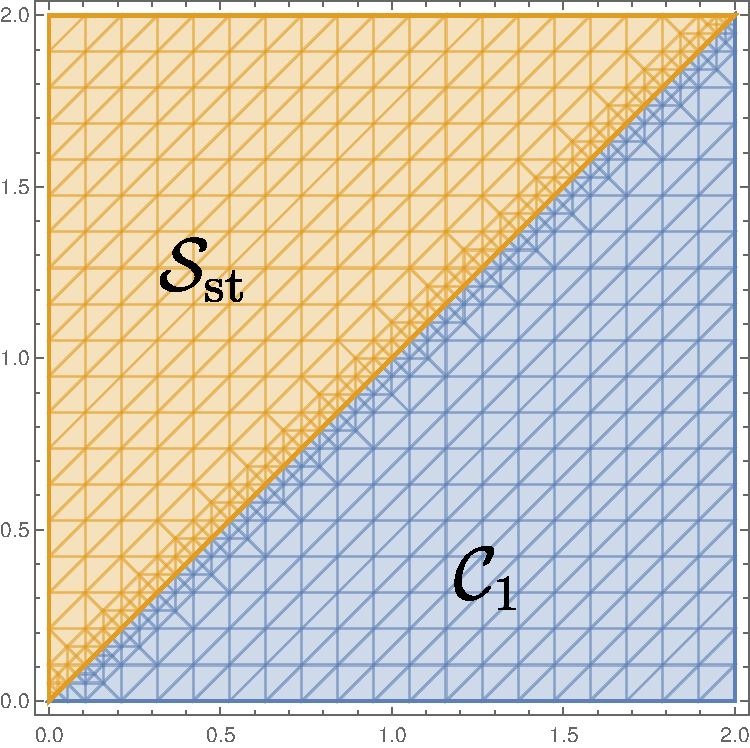
\includegraphics[width=0.3\textwidth]{Chaptersig/media/idealsfreelinear.pdf}}\label{fig.ideal.log}
  \hfill
  \subfloat[$\cSt$ and $\cC_{2}$.]{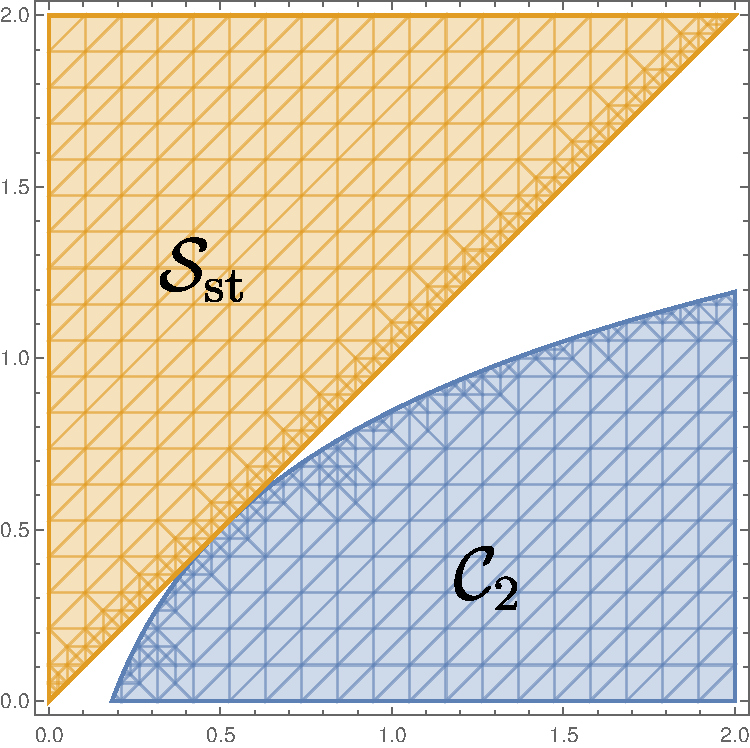
\includegraphics[width=0.3\textwidth]{Chaptersig/media/idealsfreelog.pdf}}\label{fig.ideal.power}
\hfill
  \subfloat[$\cSt$ and $\cC_{3}$.]{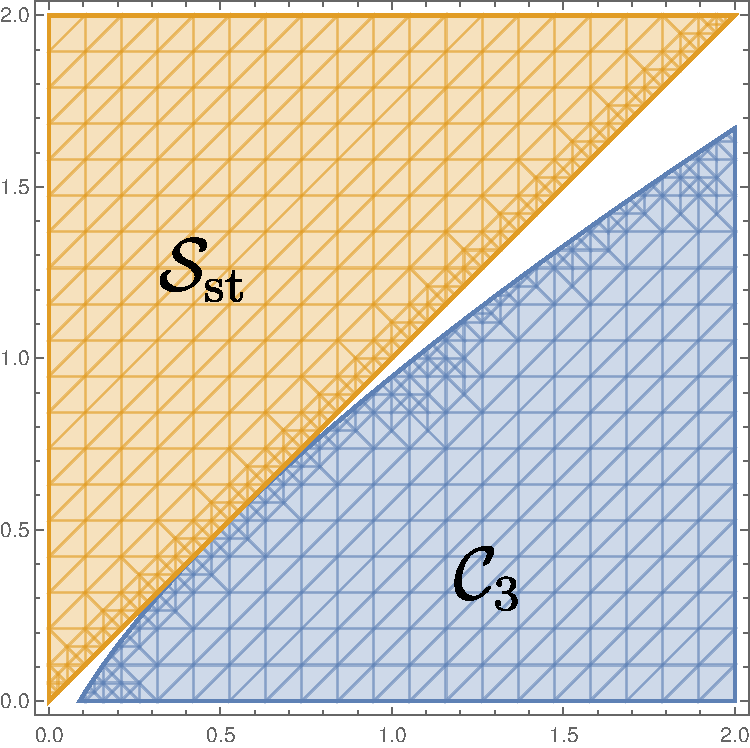
\includegraphics[width=0.3\textwidth]{Chaptersig/media/idealsfreepower.pdf}}\label{fig.exmpl.linear}
  \caption{$\cSt$-free sets.}
  \label{fig.ideal}
\end{figure}

\begin{example}
Consider the  hypograph of signomial term $x_1^{-2} x_2^{2}$ and
$
	\cSt = \{(x,y) \in \bR_{+}^3: y \le x_1^{-2} x_2^{2} \}.
$ For $(x,y) \in \bR_{++}^3$, $y \le x_1^{-2} x_2^{2}$ if and only if $ y^{1/3}x_1^{2/3} \le x_2^{2/3}$.  The following set is maximal $\cSt$-free in $\cG = \bR_+^3$:
$
	\cC_4 \deq \{(x,y) \in \bR_{+}^3:   y^{1/3}x_1^{2/3} \ge  \relx{x}_2^{2/3} + \frac{2}{3} \relx{x}_2^{-1/3} (x_2 - \relx{x}_2)\},
$
where $\relx{x}_2 \in \bR_{++}$. See \Cref{fig.free1} for $\relx{x}_2 = 0.2$.
\end{example}

\begin{example}
Consider the epigraph of signomial term $x_1^3 x_2$ and
$
	\cSt = \{(x,y) \in \bR_{+}^3: y \ge x_1^3 x_2\}.
$ For $(x,y) \in \bR_{++}^3$, $  y \ge x_1^3 x_2 $ if and only if $ y^{1/4} \ge x_1^{3/4}x_2^{1/4} $. The following set is maximal $\cSt$-free in $\cG = \bR_+^3$:
$
	\cC_5\deq \{(x,y) \in \bR_{+}^3:  \relx{y}^{1/4} + \frac{1}{4} \relx{y}^{-3/4}(y - \relx{y})\le x_1^{3/4}x_2^{1/4}  \},
$
where $\relx{y} \in \bR_{++}$. See \Cref{fig.free2} for $\relx{y} = 0.2$.
\end{example}
\begin{figure}[!ht]
 \centering
  \begin{subfigure}[b]{0.35\textwidth}
     	\centering
     	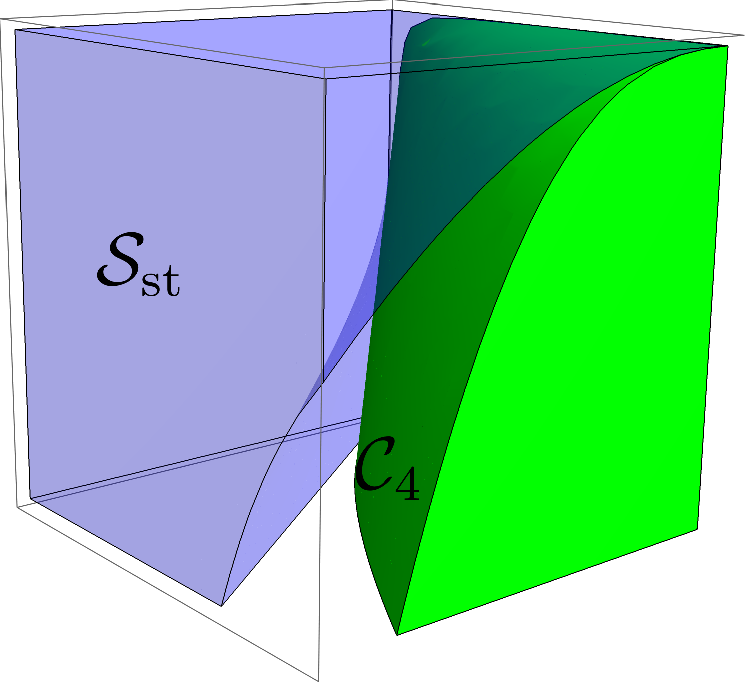
\includegraphics[width=\textwidth]{Chaptersig/media/sfree1.pdf}
     	\caption{$\cSt$ and $\cC_4$.}
    	\label{fig.free1}
 \end{subfigure}
 \hfill
  \begin{subfigure}[b]{0.35\textwidth}
     	\centering
     	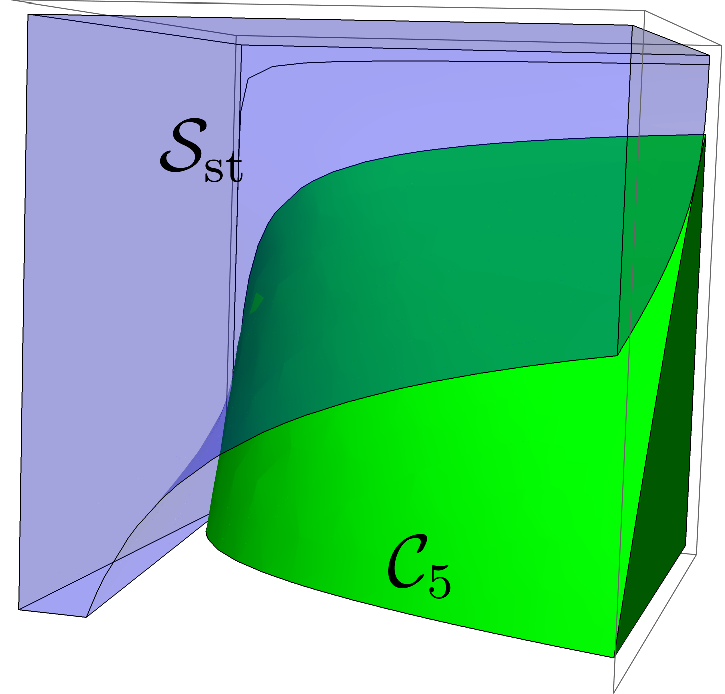
\includegraphics[width=\textwidth]{Chaptersig/media/sfree2.pdf}
     	\caption{$\cSt$ and $\cC_5$.}
    	\label{fig.free2}
 \end{subfigure}
  \caption{Two examples of $\cSt$ and $\cSt$-free sets.}
  \label{fig.free}
\end{figure}

 

\subsection{Computing intersection cuts}
\label{sec.sepic}
We focus on the separation of intersection cuts for the extended formulation of SP. In \Cref{sec.premic}, we presented a method to construct a simplicial cone $\cR$ from an LP relaxation. The vertex of that cone is  a relaxation solution $\relx{z} = (\relx{x}, \relx{y})$.

We assume that the LP relaxation includes all the linear constraints from \eqref{minlp2}. If $\relx{z}$ is not feasible for  \eqref{minlp2}, then $\relx{z}$ does not belong to the signomial lift. Hence, there exists a signomial term $g_i$ such that $\relx{y}_i \neq g_i(\relx{x})$. Given the reduced form $g'_i$,  we obtain a signomial term set $\cSt$: if $g_i(\relx{x}) > \relx{y}_i$, we choose $\cSt$ as the epigraph of $g'_i$; otherwise, we select it as the hypograph of $g'_i$.  This signomial term set yields a signomial-term-free set $\cC$ in \eqref{eq.sigfree} containing  $(\relx{u},\relx{v})$  in its interior (\Cref{cor.dc2}).  By applying the orthogonal lifting, we can transform $\cC$ into a signomial-lift-free set $\bar{\cC}$ as stated in  \Cref{cor.maxsig}.

We next show how to construct an intersection cut in \eqref{eq.ic}. It suffices to compute  step lengths $\eta^\ast_j$ in \eqref{eq.iccoef} along extreme rays $r^j$ of $\cR$. Each step length $\eta^\ast_j$ corresponds to a boundary point $\relx{z}+ \eta^\ast_j r^j$ in $\bd(\bar{\cC})$. The left-hand-side $\psi_{\beta}(u) - \lin{\psi_{\gamma}}{\relx{v}}(v)$  of the inequality in \eqref{eq.sigfree} is a concave function over $(u,v) \in \bR_{+}^h \times \bR^{\ell}$. Its  restriction along the ray $\relx{z}+ \eta_j r^j \;(\eta_j \in \bR_+)$ is a univariate concave function:
\begin{equation*}
 \tau_j:\bR_+ \to \bR, \eta_j \mapsto  \tau_j(\eta_j) \deq \psi_{\beta}(\relx{u} +  r^j_u \eta_j)  - \lin{\psi_{\gamma}}{\relx{v}}(\relx{v}+ r^j_v\eta_j),
\end{equation*}
where $r^j_u$ and $r^j_v$ are the projections of $r^j$ on $u$ and $v$ respectively. Let
$	\bar{\eta}_j \deq \sup_{\eta_j \ge 0}\{\eta_j:\relx{u} +  r^j_u \eta_j \ge 0\}$.
 Therefore, $\eta^\ast_j$ is the first point in $[0,\bar{\eta}_j]$  satisfying the boundary condition: either $ \tau_j(\eta^\ast_j) = 0$ or $\eta^\ast_j = \bar{\eta}_j$. Since  $\tau_j$ is a univariate concave function and $\tau_j(0) > 0$, there is at most one positive point in $\bR_+$ where $\tau_j$ is zero. We employ the bisection search method \cite{press2007chapter} to find such $\eta^\ast_j$.


 
 
 


\section{Convex outer approximation}
\label{sec.outerforsp}

In this section, we propose a convex nonlinear relaxation for the extended formulation \eqref{minlp3} of SP. This relaxation allows us to generate valid linear inequalities, known as outer approximation cuts, for SP. Unlike intersection cuts, outer approximation cuts do not require an LP relaxation \textit{a priori} .

Our goal is to construct a convex outer approximation of  the signomial lift. This gives rise to the convex nonlinear relaxation of SP.  To ensure the convergence of the sBB algorithm,  the feasible region of the extended formulation \eqref{minlp3} should be compact. 
Therefore, we assume that the signomial lift is in a hypercube. 

 Our algorithm approximates every signomial term set in the hypercube generated from the signomial lift. W.l.o.g., we consider a signomial term set in hypergraph or epigraph form. As \Cref{sec.siliftfree}, 
we can convert it in normalized DDC formulation:
\begin{equation}
\label{eq.st2}
	\cSt =  \{(u, v) \in \cU \times \cV:\, \psi_{\beta}(u) - \psi_{\gamma}(v) \le 0\},
\end{equation}
where $ \max(\lVert \beta \rVert_1, \lVert \gamma \rVert_1 ) = 1$, and $\cU,\cV$ are two hypercubes in $\bR_{+}^{h}, \bR_{+}^{\ell}$ respectively. The signomial term set is generally nonconvex, so we should find a convex outer approximation of $\cSt$.


Our construction involves convexifying the concave function $\psi_{\beta}$ in \eqref{eq.st2}. To do so, we will use the formal concepts of convex underestimators and convex envelopes.

Given a function  $f$ and a closed set $\cD \subseteq \bR^p$, a convex function $f':\conv(\cD) \to \bR$ is said to be a convex underestimator of $f$ over $\cD$, if, for all $x \in \cD$, $f'(x) \le f(x)$. The
 convex envelope $\conve_{\cD}(f)$  of $f$  is defined as the point-wise maximum convex underestimator of $f$ over $D$, \ie  $\epi(\conve_{\cD}(f)) = \conv(\epi_{\cD}(f))$, where $\epi_{\cD}(f) \deq \{(x,t) \in \cD \times \bR: f(x) \le t\}$.


 The following lemma gives an extended formulation of the convex envelope of a concave function over a polytope, where the formulation is uniquely determined by the function values at the vertices of the polytope. Based on \Cref{thm.poly}, we observe that the concave function $f$ is convex-extensible from its vertices (\ie $\conve_{P}(f)(x) = \conve_{Q}(f)(x)$ for $x \in P$), and $\conve_{P}(f)$ is a polyhedral function.



For the case of $P=\cU \deq \prod_{j \in [h]} [\underline{u}_j, \overline{u}_j]$ and $f =\psi_{\beta}$, $Q = \{q \in \bR^h: \forall j \in [h] \; q_j = \underline{u}_j \lor q_j = \overline{u}_j\}$ is the set of vertices of the hypercube $\cU$.  This yields an extended formulation of $\conve_{\cU}(\psi_{\beta})$. Replacing $\psi_{\beta}$ by its convex envelope $\conve_{\cU}(\psi_{\beta})$, we obtain a convex outer approximation of $ \cSt$ in \eqref{eq.st2}:
\begin{equation*}
\label{relcss}
  \bcSt\deq\{(u,v)\in \cU \times \cV: \conve_{\cU}(\psi_{\beta})(u) \le \psi_{\gamma}(v)\}.
\end{equation*}


By using this extended formulation, our convex nonlinear relaxation of SP incorporates additional auxiliary variables. Specifically, we require $2^h$ variables $\lambda_q$ to represent each convex envelope. For most SP problems in the \minlplib, where the degrees of signomial terms are less than 6, and $h$ is less than 3, the convex outer approximation remains computationally feasible.


\subsection{Outer approximation cuts}
To enhance efficiency, we propose a cutting plane algorithm to separate valid linear inequalities in the $(u,v)$-space from the extended formulation of the convex outer approximation. This algorithm generates a low-dimensional projection of $\bcSt$.



Given a point $(\relx{u}, \relx{v}) \in \cU \times \cV$, the algorithm determines whether it belongs to $\bcSt$. This verification can be done by checking the sign of $\conve_{\cU}(\psi_{\beta})(\relx{u}) - \psi_{\gamma}(\relx{v})$.  If $\conve_{\cU}(\psi_{\beta})(\relx{u}) - \psi_{\gamma}(\relx{v}) \le 0$, then $(\relx{u}, \relx{v}) \in \bcSt$. 

Since $\conve_{\cU}(\psi_{\beta})$ is a convex polyhedral function, our cutting plane algorithm evaluates the function by searching for an affine underestimator $a \cdot u+b$ of $\conve_{\cU}(u)$ such that $a \cdot \relx{u}+b = \conve_{\cU}(\relx{u})$. If $ (\relx{u}, \relx{v}) \notin \bcSt$, then   $a \cdot u+b \le  \psi_{\gamma}(\relx{v})$ is   a valid nonlinear inequality of $\bcSt$. Consequently, our cutting plane algorithm linearizes the inequality, resulting in  an outer approximation cut $a \cdot u+b \le  \lin{\psi_{\gamma}}{\relx{v}}(v)$: we recall that $\Xi$ is defined in Eq.~\eqref{def.Xi}.



 Due to \Cref{thm.poly}, we can solve the following LP to find the affine underestimator:
\begin{equation}
	\max_{a \in \bR^{h}, b \in \bR} a \cdot \relx{u}+b \quad \suc \forall q \in Q \; a \cdot q+b \le \psi_{\gamma}(q),
\end{equation}
where we omit the linear constraints that  bound $(a,b)$. The maximum value obtained from this LP  is exactly  $\conve_{\cU}(\psi_{\beta})(\relx{u})$. The affine underestimator $a \cdot \relx{u}+b$ is called a \emph{facet} of the envelope $\conve_{\cU}(\psi_{\beta})$, if $a \cdot \relx{u}+b \le t $ is a facet of $\epi(\conve_{\cU}(\psi_{\beta}))$. It should be noted that the solution of the LP is not necessarily a facet.


For $h = 1,2$, we can explicitly provide projected formulations of convex envelopes of power functions. This enables us to obtain facets of $\conve_{\cU}(\psi_{\beta})$ without the need to solve LPs. As a result, our cutting plane algorithm can efficiently separate outer approximation cuts for low-order problems.

To simplify our presentation, we translate and scale the domain of $\psi_{\beta}$ to $[0,1]^h$. This yields a new function $s(w) \deq \psi_{\beta}(u)$, where for all $j \in [h]$, $u_j \deq \overline{u}_j + (\overline{u}_j - \underline{u}_j)w_j$. After these transformations, we have $\cU = [0,1]^h$ and $Q = \{0,1\}^h$.   W.l.o.g., we focus on studying and computing facets of $\conve_{\cU}(s)$. For $h = 1$, the only facet is $s(0) + (s(1)- s(0))w_1$. 


 A set $D \subseteq \bR^h$ is called a \emph{product set}, if  $D = \bigtimes_{j \in [h]}D_j$ for $D_j \subseteq \bR$. Let $D$ be a product set. A function $f: D  \to \bR$ is \emph{supermodular} over $D$ (Section 2.6.1 of \cite{topkis2011supermodularity}), if the increasing difference condition holds:
for all $w^1,w^2 \in D, d \in \bR^h_{+}$ such that $w^1 \le w^2 $ and $ w^1+d, w^2+d \in D$, $f(w^1+d) -f(w^1)\le f(w^2 + d) -f(w^2)$. 
The following operations preserve supermodularity. 

\begin{lemma}
\label{lem.subtrans}
    Let $w' \in \bR^h, \rho \in \bR^h_{++}$,  and let $D'$ be a product subset of $D$. The following results hold: (restriction) $f$ is supermodular over $D'$;(translation) $ f(w+w')$ is supermodular over $D-d$; (scaling) $f(\rho * w)$ is supermodular over $D/\rho$, where $+, -, *, /$ are taken entry-wise.
\end{lemma}
\begin{proof}
    The results follow from the definition.
\end{proof}


 We note that when $D= Q$, $d$ is in $Q$.  We observe a useful property of $g$. 
 
\begin{proposition}
\label{lem.sup}
$s$ is supermodular over $Q$ and $\conve_{\cU}(s) = \conve_{\cQ}(g)$.
\end{proposition}
\begin{proof} 
According to Example 2.6.2 of \cite{topkis2011supermodularity}, the signomial term
$\psi_\alpha$ with $\alpha > 0$ is a Cobb-Douglas function, which is supermodular  over $\bR^h_{+}$. This implies that the power function $\psi_\beta$ is supermodular over $\bR^h_+$. By \Cref{lem.subtrans}, $s$ is supermodular over $\cU = [0,1]^h$. As $Q=\{0,1\}^h$ is a product subset of $\cU$,   $s$  is supermodular over $Q$. After the scaling and translation, $s$ is still concave, so it follows from \Cref{thm.poly} that $\conve_{\cU}(s) = \conve_{\cQ}(s)$.
\end{proof}

The search for facets of $s$ can be reduced to a more general problem, which involves finding facets of supermodular functions over  Boolean hypercubes.

We note that both power functions and multilinear terms can be considered Cobb-Douglas functions. Consequently, a similar argument can be used to demonstrate that multilinear terms are supermodular over any product subset of $\bR^h_+$.
  
\subsection{Convex envelopes of bivariate supermodular functions}

 
 Using the aforementioned result in \Cref{sec.conenvesuper}, we can construct an envelope-inducing family for bivariate supermodular functions. Let 
\begin{equation}
\label{eq.induce2}
    S^2_1 \deq \{00,10,01\}, S^2_2 \deq 
     \{11,10,01\}.
\end{equation}
One can find that $\conv(S^2_1)=\{(w_1,w_2) \in [0,1]^2:w_1 + w_2 \le 1 \}, \conv(S^2_2)=\{(w_1,w_2) \in [0,1]^2: w_1 + w_2 \ge 1 \}$ are two triangles in $[0,1]^2$.  We have that 
     	\begin{align*}
    	& f_{S^2_1}(w) =  f(00) + (f(10) -f(00)) w_1 + (f(01) -f(00)) w_2,\\
    	& f_{S^2_2}(w) = f(11) + (f(01) -f(11)) (1 - w_1) + (f(10) -f(11)) (1 - w_2).
	\end{align*}
 We show that these two affine functions define the convex envelope of $f$.
 
 \begin{theorem}
     For $h = 2$, $\{S^2_k\}_{k \in [2]}$ as in \eqref{eq.induce2}  is  envelope-inducing family in $Q$.
 \end{theorem}
 \begin{proof}
 It is easy to see that for all $k \in [2]$, $S^2_k$ is affinely independent and $\{\conv(S^2_k)\}_{k \in [2]}$ is a triangulation of $\cU$.  Therefore, it suffices to show that $\{S^2_k\}_{k \in [2]}$  is facet-inducing, \ie $f_{S^2_1}, f_{S^2_2}$ are affine underestimators of $f$. 
 
 \textbf{Case i.}
 We note that for all $w \in S^2_1 = \{00,10,01\}$, $f_{S^2_1}(w) = f(w).$ Note that $Q\smallsetminus S^2_1 = \{11\}.$ It follows from the definition of the affine function $f_{S^2_1}$  that
 \begin{equation*}
     f_{S^2_1}(11)= f_{S^2_1}(10) + (f_{S^2_1}(01) - f_{S^2_1}(00)) = f(10) + (f(01) - f(00)).
 \end{equation*}
 It follows from the supermodularity of $f$ that 
 \begin{equation*}
     f(10) + (f(01) - f(00)) \le  f(10) + (f(11) - f(10)) = f(11).
 \end{equation*}
 Thereby, $f_{S^2_1}$ underestimates $f$.

  \textbf{Case ii.}
 We note that for all $w \in S^2_2 = \{11,10,01\}$, $f_{S^2_2}(w) = f(w).$  Note that $Q\smallsetminus S^2_2 = \{00\}.$ It follows from the definition of the affine function $f_{S^2_2}$  that
 \begin{equation*}
     f_{S^2_2}(00)= f_{S^2_2}(10) - (f_{S^2_1}(11) - f_{S^2_1}(01)) = f(10) + (f(11) - f(01)).
 \end{equation*}
 It follows from the supermodularity of $f$ that 
 \begin{equation*}
     f(10) - (f(11) - f(01)) \le  f(10) - (f(10) - f(00)) = f(00),
 \end{equation*}
which concludes the proof.
 \end{proof}



 \subsection{Convexity and reverse-convexity}
 \label{sec.conv}
Our cutting algorithm can detect the convexity/reverse-convexity of signomial term sets. The detection is simply through  normalized  DDC formulations.

Denote by $e^\ell_j$ and $e^h_j$ the $j$-th unit vector in $\bR^h$ and $\bR^\ell$ respectively. Then, we have the following observations:
\begin{enumerate}
	\item[i)] if $\norm{\beta}_1 = 1,\gamma = 0$, \ie $\psi_{\beta}$ is concave and $\psi_{\gamma}$ is 1, then $\cSt$ is reverse-convex;
	\item[ii)] if $\norm{\beta}_1 \le 1,\gamma = e^\ell_j$ for some $j \in [\ell]$, \ie $\psi_{\beta}$ is concave and $\psi_{\gamma}$ is a linear univariate function, then $\cSt$ is reverse-convex;
   \item[iii)] if $\beta = e^h_j, \norm{\gamma}_1 \le 1$ for some $j \in [h]$, \ie
$\psi_{\beta}$ is a linear univariate function and $\psi_{\gamma}$ is concave, then  $\cSt$ is convex;
   \item[iv)] if $\norm{\beta}_1 = 0, \norm{\gamma}_1 = 1$, \ie $\psi_{\beta}$ is 1  and $\psi_{\gamma}$ is concave, then $\cSt$ is convex.
\end{enumerate}

We note that similar results are found in \cite{chen2009note,maranas1995finding}. The results in  \cite{chen2009note} are proved by checking the negative/positive-semidefiniteness of the Hessian matrix of a signomial term. According to the normalized DCC formulation, the results are evident.



\section{Computational results}
\label{sec.comp}


In this section, we conduct computational experiments to assess the efficiency of the proposed valid inequalities.



The \minlplib dataset comprises instances of MINLP problems that involve signomial terms, and some of these instances are SP problems. To build our benchmark, we select instances from \minlplib that satisfy the following criteria: (i) the instance includes signomial functions or polynomial functions, (ii) the continuous relaxation of the instance is non-convex. Our benchmark consists of a diverse set of 251 instances in which nonlinear functions consist of signomial and other functions. These problems frequently arise in practical applications and are commonly solved by general-purpose solvers.

Experiments are conducted on a server with  Intel Xeon W-2245 CPU @ 3.90GHz, 126GB main memory, and Ubuntu 18.04 system.  We use \scip 8.0.3 \cite{bestuzheva2023global}  as the framework for reading and solving problems, as well as conducting cut separation. \scip is integrated with \texttt{CPLEX} 22.1 as LP solver and \texttt{IPOPT} 3.14.7 as  NLP solver.


We evaluate the efficiency of the proposed valid inequalities in four different settings. The first setting, denoted as \disable, does not apply any of the proposed valid inequalities. The second setting, denoted as \oc, applies only the outer approximation cuts. The third setting, denoted as \ic, applies only the intersection cuts. The fourth setting combines both the \oc and \ic settings by applying both cuts.  We let \scip's default internal cuts to handle univariate signomial terms and multilinear terms. Our valid inequalities only handle the other high-order signomial terms.  The source code, data, and detailed results can be found in our online repository: \href{https://github.com/lidingxu/ESPCuts}{github.com/lidingxu/ESPCuts}.


In our benchmark, there are 150 instances classified as \emph{affected}, in which at least one of the \oc, \ic, and \oic settings adds cuts. There are 86 instances among the affected ones, for which \scip's default configuration (\ie the \disable setting) runs at least 500 seconds. Such instances are classified as \emph{affected-hard}. Each test run uses \scip configured by a setting to solve an instance. To solve the instances, we use the \scip solver with its sBB algorithm, imposing a time limit of 3600 seconds. For each test run, we measure the running time, the number of sBB search nodes, and the relative open duality gap.


To aggregate the performance metrics for a given setting, we compute shifted geometric means (SGMs) over our test set. The SGM for the running time incorporates a shift of 1 second. The SGM for the node number incorporates a shift of 100 nodes. The SGM for the relative gap incorporates a shift of 1$\%$. We  also compute SGMs of   performance metrics over the subset of affected and affected-hard instances. The performance results are presented in  \Cref{tb.perf}, where we also compute the relative values of SGMs of  performance metrics compared to the \disable setting. Our following analysis is based on the results on affected and affected-hard instances.





\begin{table} [htbp]
\centering
\resizebox{\columnwidth}{!}{
\addtolength{\tabcolsep}{-0.28em}
\begin{tabular}{cc|*{4}{c}|*{4}{c}|*{4}{c}}
\toprule
\multicolumn{2}{c|}{\multirow{2}{*}{Setting}}  &
\multicolumn{4}{c|}{All}    &
\multicolumn{4}{c|}{Affected} &
\multicolumn{4}{c}{Affected-hard}  \\
& &
{solved} &
{nodes}     &
{time} &
{gap}     &
{solved} &
{nodes}     &
{time} &
{gap}   &
{solved} &
{nodes}     &
{time} &
{gap}   \\
\midrule
\multirow{2}{*}{\disable} & absolute  & \multirow{2}{*}{138/251} &  6510.5 & 122.0 & 4.7\%  & \multirow{2}{*}{71/150} &  15592.4 & 253.6 & 5.7\% & \multirow{2}{*}{7/86} & 175973.8 & 3600.0 & 26.7\%  \\ 
 & relative &  & 1.0 & 1.0 & 1.0 & & 1.0 & 1.0 & 1.0 & & 1.0 & 1.0 & 1.0 \\
 \midrule
\multirow{2}{*}{\oc} & absolute  & \multirow{2}{*}{140/251}  &  5954.1 & 118.0 & 4.5\%  & \multirow{2}{*}{73/150} & 13443.9 & 241.4 & 5.4\% &  \multirow{2}{*}{10/86} & 115262.3 & 2872.7 & 23.3\%   \\ 
 & relative &  &    0.91 & 0.97 & 0.97 & & 0.86 & 0.95 & 0.95 & & 0.65 & 0.8 & 0.87 \\
 \midrule
 \multirow{2}{*}{\ic} & absolute  & \multirow{2}{*}{140/251} & 6144.3 & 122.4 & 4.4\% & \multirow{2}{*}{73/150} &  14081.5 & 252.1 & 5.2\% & \multirow{2}{*}{10/86} & 128072.7 & 2994.1 & 22.0\%  \\ 
 & relative &  & 0.94 & 1.0 & 0.95 & &  0.9 & 0.99 & 0.91 &  & 0.73 & 0.83 & 0.82\\
 \midrule
 \multirow{2}{*}{\oic} & absolute  & \multirow{2}{*}{139/251} &  5934.6 & 117.7 & 4.6\% &  \multirow{2}{*}{72/150} & 13275.6 & 236.8 & 5.6\% & \multirow{2}{*}{10/86}  & 118054.1 & 2758.3 & 23.0\%\\ 
 & relative &  &  0.91 & 0.96 & 0.99 & & 0.85 & 0.93 & 0.98 &  & 0.67 & 0.77 & 0.86\\
\bottomrule
\end{tabular}
}
\caption{Summary of performance metrics on \minlplib instances}\label{tb.perf}
\end{table}





First, we observe that  the proposed valid inequalities lead to the successful solution of 2 additional instances compared to the \disable setting. Considering the \oc setting, it solves 2 more instances than the \disable setting. Note that, in the affected-hard  benchmark, the number of solved instances by any non-disable setting is 3 more than that by the disable setting; in the affected  benchmark, the number of solved instances by any non-disable setting is at most 2 more than that by the disable setting. This is because restriction of the benchmark can reduces more solvable instances by the disable setting. 

The reductions in the running time, and relative gap achieved by the  \oc setting are  respectively  5\%, 5\% for affected instances and  20\%, 13\% for affected-hard instances. For the \ic setting, it solves 2 more instances than the \disable setting. The reductions in the running time, and relative gap achieved by the \ic setting are  respectively  1\%, 9\% for affected instances and 17\%, 14\% for affected-hard instances. In the case of the \oic setting, it solves 1 additional instance compared to  the \disable setting. The reductions in the running time, and relative gap achieved by the \oic setting are respectivel 7\%,  2\% for affected instances and  23\%, 14\% for affected-hard instances.

We note that the running time  does not give much information on affected-hard instances, because only 10 instances can be solved within 3600 seconds. For these instances, the gap reduction is more useful to measure the reduction of the search space by the proposed valid inequalities. However, for all affected instances, the running time  is still important, as it measures the acceleration by the valid inequalities. 

Secondly, we observe that all cut settings have a positive impact on the performance of \scip, although the extent of reduction varies. When comparing the \oc and \ic settings, we find that the \oc setting leads to a greater reduction in running time. This difference in running time arises because computing intersection cuts involves extracting a simplicial cone from the LP relaxation and applying bisection search along each ray of the cone. These procedures require more computational resources compared to the construction of outer approximation cuts.


On the other hand, the \ic setting demonstrates better performance in terms of gap reduction. Intersection cuts approximate the intersection of a signomial term set with the simplicial cone, while outer approximation cuts approximate the intersection of a signomial term set with a hypercube. Around the relaxation point, the simplicial cone typically provides a better  approximation than the hypercube. Hence, \ic achieves a larger reduction in the relative gap. However, the better simplicial conic approximation does yield a significant improvement compared to the hypercubic approximation.

Lastly, the \oic setting combines both the \oc and \ic settings, achieving the best reduction in the running time. However, for affected and affected-hard instances, the setting exhibits different results on gap reduction. In fact, the results of 
affected-hard instances give more insights, since the goal of valid inequalities is to accelerate the convergence for had instances. In this sense, the \oic setting achieves nearly the best result,  so it inherits the best of both valid inequalities.  However, its improvement compared to the individual settings is not significant.

To summarize, the performances of  the \oc and \ic settings are comparable. They can lead to smaller duality gap with less computational time, which are desirable for solvers, and one can use any of them. Moreover,  they do not hurt each other.



\section{Conclusion}

In this chapter, we study valid inequalities for SP problems, and propose two types of valid linear inequalities: intersection cuts and outer approximation cuts.  They are both derived from the normalized DCC formulations of signomial term sets. First, we study general conditions on maximal $\cS$-free sets. We construct maximal signomial-term-free sets, from which we  generate   intersection cuts. Secondly, we construct  convex outer approximations of signomial term sets within hypercubes. We provide extended formulations for the convex envelopes of the concave functions in the normalized DCC formulations. Then we separate valid inequalities for the convex outer approximations through projection.  Additionally, when $h=2$, we use supermodularity to derive a closed-form expression for the convex envelopes.
 

We present a comparative analysis of computational results obtained from the \minlplib instances. This analysis demonstrates the effectiveness of the proposed valid inequalities. The results indicate that intersection cuts and outer approximation cuts exhibit similar performance, and their combination inherits the best of the individual settings. In particular, it is straightforward to  implement outer approximation cuts in general-purpose solvers.  In the future, we intend to carefully fine-tune outer approximation cuts  and develop it as an easy-to-use plugin. 

We currently deal with signomial terms that explicitly present in the signomial lift, but our results can be extended to handle more ``faces'' of the signomial lift. In the future, the proposed valid inequalities can  approximate nonlinear aggregations of  constraints defining the signomial lift. Specifically, given signomial constraints $\{\psi_{\alpha^i}(x) = y_i\}_{i \in [r]}$, with  any exponent vector $\zeta \in \bR^r$, we can employ \emph{signomial aggregation} to generate a new signomial constraint: $\psi_{(\sum_{i \in [r]}\zeta_i\alpha^i)}(x) = \psi_{\zeta}(y)$. This constraint is valid for the signomial lift and encodes more variables and terms. Subsequently, we can apply DCC reformulation to the constraints  $\psi_{(\sum_{i \in [r]}\zeta_i\alpha^i)}(x) \le \psi_{\zeta}(y)$ and $\psi_{(\sum_{i \in [r]}\zeta_i\alpha^i)}(x) \ge \psi_{\zeta}(y)$. Finally, we can separate the proposed valid inequalities. As far as we know, the signomial aggregation operator is not used yet for polynomial programming, as it outputs a signomial constraint.




% ===============================================
% ===============================================





































\chapter{Intersection cuts for submodular optimization}
\label{chap.submax}




\section{Introduction}


  In this chapter, we first consider $\cS$ as the Boolean-hypograph $\hyp_{\{0,1\}^n}(f)$ of $f$. We use convex extensions of $f$ in order to construct some $\cS$-free sets, which we call \textit{Boolean-hypograph-free}. The Boolean-hypograph set $\hyp_{\{0,1\}^n}(f)$ is a specialization of the constraint set $\{(x, t) \in \{0,1\}^n \times \bR: f_1(x) -f_2(x)  \ge \ell t\}$
with $ \ell \in \{0,1\}$. Then, we consider $\cS$ as this general constraint set and extend our results to handle this  general case. Finally, we propose an efficient algorithm to compute intersection cuts derived from $\cS$-free sets. To the best of our knowledge, intersection cuts have not  been applied directly to approximate problems with submodular and/or supermodular structures.

We implement intersection cuts within the \scip solver \cite{bestuzheva2021scip} and test them on \maxcut,  \pbm, and  \bdopt problems. We show the strengths and weaknesses of intersection cuts under these different settings.




\subsection{Literature review}

 
 
The \textit{base inequalities} \cite{nemhauser1978analysis} are a class of valid linear inequalities for the hypographs of general submodular functions. For a class of special submodular functions, lifting procedures  \cite{ahmed2011maximizing,shi2022sequence}  can strengthen the base inequalities. The  base inequalities can be separated either using heuristics \cite{ahmed2011maximizing} or a Benders-like framework \cite{coniglio2022submodular} if the point to be separated is integer. The method defined in \cite{Atamturk2021} combines valid inequalities for the submodular and supermodular components of an SS function. We refer to \cite{atamturk2020submodularity,atamturk2022supermodularity2,billionnet1985maximizing,bouhtou2010submodularity,han2022fractional,kilincc2021joint,rhys1970selection,shamaiah2010greedy,xusignomial,yu2023strong} for more details about the exploitation of  submodular/supermodular functions in mathematical programs. Supermodular polynomials in binary variables are defined and studied in \cite{billionnet1985maximizing,rhys1970selection}. The submodularity of the \dopt problem is exploited in \cite{SAGNOL2013258,shamaiah2010greedy}.


As already mentioned, intersection cuts generate valid inequalities for sets that are hard to optimize over. Gomory introduced the corner polyhedron \cite{gomory1969some}, and his celebrated mixed-integer cuts \cite{gomory1963algorithm} are special intersection cuts derived from split disjunctions \cite{Nemhauser1988}. The definition of intersection cuts for arbitrary set $\cS$ is due to \cite{dey2008,glover1973}. We refer to  \cite{andersen2010,andersen2007,basu2010,basu2019,conforti2015,conforti2011,cornuejols2015sufficiency,del2012relaxations,dey2008,richard2010group} for a more in-depth analysis.  The method given in \cite{towle2021intersection} can generate valid inequalities that cut off points outside $\cS$-free sets. We refer to \cite{andersen2007,belotti2015conic,klnc-karzan2015,kilinc-karzan2016,modaresi2015,modaresi2016} for relevant recent developments in mixed-integer conic programming.

For the cases where the nonconvexity of $\cS$ is not just due to integer variables, we refer to \cite{fischetti2018} for bilevel programs, \cite{bienstock2020outer} for outer-product sets, \cite{munoz2020maximal,munoz2022towards} for quadratic constraint sets, \cite{xusignomial} for signomial-term sets, and \cite{fischetti2020} for bilinear sets. The method given in \cite{serrano2019} constructs intersection cuts  for sets arising from factorable programs that contain DC functions \cite{khamisov1999optimization}.
 
 
Next, we discuss valid inequalities for polynomial programming, because we use polynomial programs in binary variables as a benchmark in our computational study. In \cite{bienstock2020outer}, intersection cuts approximate a nonconvex lifted set, namely the outer product set arising from  the extended formulation of a polynomial program. Lifted sets link decision variables to auxiliary variables representing (graphs of) monomials up to a given degree. We remark that in most combinatorial optimization problems,  decision variables are binaries. The polynomial program of interest is then a Boolean Multilinear Program (BMP).  The corresponding lifted set is the \textit{Boolean multilinear set} \cite{crama1993concave,fortet1960applications}, the convex hull of which is the so-called Boolean multilinear polytope. Valid inequalities for the Boolean multilinear polytope may be stronger than those for the  convex  hull of the outer product set. Various Gomory-Chvátal-based inequalities \cite{del2017polyhedral,del2018multilinear,del2020impact,del2022simple} are valid for the multilinear polytope. The separation and strength of these inequalities depend on  the hypergraph representing the underlying sparsity pattern of the multilinear set.

 We consider a constrained polynomial program, and assume that some  of its constraints are neither integrality constraints nor variable bound constraints. After lifting,  those constraints are linear and  thus define a convex set $\cS_1$. The lifted set $\cS_2$ is nonconvex, and $\cS_1 \not\subseteq \cS_2$.  The polynomial program is then equivalent to linear optimization over $\conv(\cS_1 \cap \cS_2)$. However, in general, $\conv(\cS_1 \cap \cS_2) \ne \cS_1 \cap \conv(\cS_2)$, so the convexification of the lifted set may not yield an equivalent convex problem. To address this issue, one attempt is to directly consider $\conv(\cS_1 \cap \cS_2)$ and generate valid inequalities for it.  Some work in this sense exists for certain interesting special cases, e.g.~the intersection of multilinear sets with additional constraint sets such as cardinality constraints \cite{chen2023multilinear}. Another attempt is to consider  constraints in projected formulations, \eg in mixed-integer quadratically constrained quadratic programs \cite{saxena2011convex}. Since the  representation complexity  of the projected formulation  is smaller than that of the  extended formulation, this approach is also amenable to computation. In \cite{chmiela2022implementation,munoz2020maximal}, intersection cuts for the set defined by a quadratic constraint are derived. If additionally, some of the nonbasic variables of the LP relaxation need to be integer, the monoidal technique \cite{ChmielaMunozSerrano2023} can strengthen such intersection cuts.

 
However, generating valid inequalities for Boolean multilinear constraints, and, more generally, constructing $\cS$-free sets for nonlinear constraints on discrete variables, remain problems of considerable interest. In this chapter, we look at these questions through a ``submodularity lens''.


\subsection{Contribution}
In \Cref{sec.freeforsub}, we already studied vairous properties for $\cS$-free sets arising in submodular maximization. We summarize those theoretical contributions here.
Our primary contribution is the construction of Boolean-hypograph-free sets. We show that a maximal Boolean-hypograph-free set $\cC \times \bR$ can be lifted from  a maximal $\{0,1\}^n$-free set.  We also give an alternative construction of Boolean-hypograph-free sets by exploiting  the submodularity. We relate the analytical properties of  $\bsF_{f}$ in \eqref{eq.bsf_f} to its combinatorial properties, which inherit those of the Lovász extension. We show that the epigraph $\epi(\bsF_{f})$ of $\bsF_{f}$ is a Boolean-hypograph-free set that is  larger than the epigraph of the Lovász extension. However, unlike in the continuous setting, $\epi(\bsF_{f})$ is not maximally Boolean-hypograph-free. We give necessary and sufficient conditions on maximal  Boolean-hypograph-free sets that contain $\epi(\bsF_{f})$.

The second contribution is  the computation of intersection cuts. We reduce the intersection cut separation problem to solving univariate nonlinear equations, which we achieve by a hybrid discrete Newton algorithm like \cite{Goemans}. We show that facets of $\epi(\bsF_{f})$ can be separated in strongly polynomial time. This implies that the (sub)-gradients required by the  Newton algorithm can be computed in a strongly polynomial time. The hybrid discrete Newton algorithm finds a zero point of a univariate nonlinear equation  in a finite number of steps. By contrast, the conventional bisection algorithm  only guarantees $\epsilon$-approximated solutions for $\epsilon > 0$.
 

Lastly, we  extend the previous findings to constraint sets involving an SS function. We show that any Boolean multilinear function is an SS function. This result yields intersection cuts for multilinear constraints in binary variables.


\subsection{Outline of the chapter}
The rest of the chapter is organized as follows. In \Cref{sec.app}, we consider applications for intersection cuts to Boolean multilinear constraints and \bdopt. In \Cref{sec.sep}, we propose the hybrid discrete Newton algorithm for computing intersection cuts. In \Cref{sec.cresult}, we analyze the computational results.


\section{Application}
\label{sec.app}
In this section, we discuss the application of intersection cuts to Boolean multilinear programming and D-optimal design. We exploit the submodular structures in these two problems.


\subsection{Boolean multilinear constraints}
\label{sec.bmc}
We consider the construction of $\cS$-free sets for Boolean multilinear constraints.
Since $x\in\{0,1\}\Leftrightarrow x^2=x$, one can reduce a  polynomial function defined on binary variables to a  multilinear  function, whose monomials do not include powers. For example, $x_1^2x_3^3+x_2^2$ can be reduced to $x_1x_3+x_2$.   A Boolean multilinear function is sometimes called a pseudo Boolean function.


 A similar case is the construction of $\cS$-free sets  for continuous quadratic constraints \cite{munoz2020maximal}. We call this construction the ``continuous approach''. It applies eigenvalue decomposition to factor the symmetric matrix representing quadratic terms in a quadratic constraint. Through this factorization, the quadratic constraint is reformulated to a DC constraint, possibly intersected with additional linear constraints. This reformulation is amenable to the reverse-linearization technique. Applying the technique with possibly additional operations, one can construct the so-called continuous-quadratic-free sets  \cite{munoz2020maximal} \footnote{The construction is \textit{de facto} discussed case by case. For some cases,  the reverse-linearization technique already suffices to produce continuous-quadratic-free sets. For other cases, one needs additional operations, \eg projecting out a lineality space. Notably, all cases require the eigenvalue decomposition and its resulting DC constraint.}. Multilinear terms, however, are represented by tensors. High-order tensor decomposition is  more complicated than matrix decomposition \cite{kolda2009tensor}. It is doubtful whether the continuous approach can be extended so as to produce DC functions from tensors.
 
Here we consider an alternative discrete approach. It exploits the submodularity and the supermodularity of Boolean multilinear functions. In \cite{billionnet1985maximizing,nemhauser1978analysis}, a class of Boolean multilinear functions is shown to be supermodular. We give a submodular-supermodular decomposition for general Boolean multilinear functions in the following.

\begin{proposition}
\label{lem.supml}
Consider a Boolean multilinear function $f: \cB \to \bR, x \mapsto \sum_{k \in [K]} a_k \prod_{j \in A_k}x_j$  with $K$ multilinear terms, where  $A_k \subseteq [n]$. Let $f = f_1 - f_2$ where
\begin{eqnarray}
    f_1(x) &:=& \quad \sum\limits_{k \in [K]\atop a_k < 0} a_k \prod\limits_{j \in A_k}x_j \label{prop9a}\\
    f_2(x) &:=& -\sum\limits_{k \in [K]\atop a_k > 0} a_k \prod\limits_{j \in A_k}x_j.\label{prop9b}
\end{eqnarray}
Then  $f_1,f_2$ are submodular over $\cB$.
\end{proposition}
\begin{proof}
It follows from Theorem 13.21 of \cite{crama2011boolean} that $f_1,f_2$ are submodular functions over $\cB$.\end{proof}


Since every Boolean multilinear function is an SS function, we can construct $\cS$-free sets for the corresponding Boolean-superlevel set or Boolean-hypograph set.

\begin{corollary}
\label{prop.bm}
Consider a  multilinear function $f: \cB \to \bR$, where $f(x) = \sum_{k \in [K]} a_i \prod_{j \in A_k}x_j$ for $A_k \subseteq [n]$ as in \Cref{lem.supml}, and $f_1(x),f_2(x)$ as in Eq.~\eqref{prop9a}-\eqref{prop9b}. 
%Let $f_1(x):=\sum_{k \in [K]\atop a_k < 0} a_k \prod_{j \in A_k}x_j$ and $f_2(x):=\sum_{k \in [K]\atop a_k > 0} -a_k \prod_{j \in A_k}x_j$.  
Let $\cS$, $\overline{\cS}$, and $\cC_{\relx{x}}$ be as \eqref{eq.cs}, \eqref{eq.csb}, \eqref{eq.c}, respectively. Then, the set $\cC_{\relx{x}}$ is an $\cS$-free set. Moreover, if $\relx{x} \notin \overline{\cS}$, then $\cC_{\relx{x}}$ does not contain $\relx{x}$ in its interior.
\end{corollary}
\begin{proof}
By \Cref{lem.supml}, we know that both $f_1$ and $f_2$ are submodular. Hence, the result follows by applying  \Cref{prop.dsfree}.
\end{proof}


Importing the notation in \Cref{lem.supml}, a BMP problem has the following form:
\begin{subequations}
\label{bmp}
\begin{alignat}{2}
	\max &&\quad t \\
&& \quad \sum_{k \in \cK_0} a_{ik} \prod_{j \in A_k}x_j &\ge  t  \label{bmp.obj}\\
  \forall i \in  [m] && \quad \sum_{k \in \cK_i} a_{ik} \prod_{j \in A_k}x_j & \ge 0  \label{bmp.cons}\\
  \forall  j \in [n] && \quad 	x_j  & \in \{0,  1\},
\end{alignat}
\end{subequations}
where $m$ is the number of constraints, $K$ is the number of  distinct multilinear terms in the BMP, $\cK_i \subseteq [K]$ is the index set of multilinear terms in the $i$-th constraint ($0$ for objective). Unconstrained BMP has several synonyms: \pbm  or \textsc{multilinear unconstrained binary optimization (MUBO)}.


To construct $\cS$-free sets for Boolean multilinear constraints in the BMP, we need to write them  as the standard form \eqref{eq.cs}.
For all $i \in [m]$ or $i = 0$, let $$f_i(x) := \sum_{k \in \cK_i} a_{ik} \prod_{j \in A_k} x_j,$$ and write $$f_i(x)= f_{i1}(x) - f_{i2}(x),$$ where $f_{i1}:= \sum_{k \in \cK_i:a_{ik} < 0} a_{ik} \prod_{j \in A_k} x_j$ and $f_{i2}:= -\sum_{k \in \cK_i:a_{ik} > 0} a_{ik} \prod_{j \in A_k} x_j$ are two  submodular functions.  

The objective and constraints of \eqref{bmp} can be represented as $$f_{i1}(x) - f_{i2}(x) \ge \ell_i t$$ (for all $i \in [m]$, $\ell_i = 0$, and $\ell_0$ = 1), which, by \Cref{prop.bm}, is in the standard form.  


Separating intersection cuts requires LP relaxations or simplicial cones.
 One can first lift multilinear terms to obtain an extended formulation:
 \begin{subequations}
\label{eq.bmplift}
\begin{alignat}{2}
	\max && \quad t\\
&& \quad \sum_{k \in \cK_0} a_{0k}  y_k &\ge  t  \label{bmplift.obj}  \\
  \forall i \in  [m] && \quad \sum_{k \in \cK_i} a_{ik}  y_k & \ge 0  \label{bmplift.cons}\\
	\quad  k \in [K] && \quad y_k &=  \prod_{j \in A_k}x_j \label{bmplift.monomial} \\
     \forall  j \in [n] && \quad 	x_j &\in \{0,  1\}
\end{alignat}
\end{subequations}

The standard Boolean linearization technique  \cite{crama1993concave} can reformulate a  multilinear term $\prod_{j \in A_k}x_j $ by  its underestimators and overestimators:
 \begin{subequations}
 \label{eq.stdlinear}
\begin{alignat}{2}
    \forall j \in A_k && \quad y_k  & \le x_j  \label{eq.stdlinear.over}\\
           		 && \quad  y_k  & \ge |A_k| + 1 - \sum_{j \in A_k} x_j \label{eq.stdlinear.under},
\end{alignat}
\end{subequations}
where $|A_k|$ is the cardinality of $A_k$. Then,  by linearizing each nonlinear constraint \eqref{bmplift.monomial}  as linear constraints in \eqref{eq.stdlinear}, one obtains a MILP reformulation of \eqref{eq.bmplift}.

To construct LP relaxations,  one can simply drop the integrality constraints $x_j \in \{0,1\}$. The direct LP relaxation of the MILP reformulation is also  an  LP relaxation of the BMP \eqref{eq.bmplift}. Following the method at the end of  \Cref{sec.maxsub},  we can construct an optimal tableau cone in the extended space $(x,y,t)$. The $\cS$-free set belongs to a projected space (\ie $(x,t)$-space). By extracting the $(x,t)$ entries of the rays of the optimal tableau cone, we  project the optimal tableau cone into the $(x,t)$-space. Given the projection of this optimal tableau cone, it is straightforward to construct intersection cuts for the BMP: we  separate the intersection cuts constructed by means of the $\cS$-free sets given by \Cref{prop.dsfree}.
 
As explained above, Boolean quadratic constraints belong to Boolean multilinear constraints, and continuous  quadratic constraints relax Boolean quadratic constraints. Both the continuous and discrete approaches can construct valid $\cS$-free sets for Boolean quadratic constraints. We remark that  maximal continuous-quadratic-free sets are no longer maximally Boolean-quadratic-free. It is easy to see that the  discrete approach  preserves the term-wise sparsity patterns of the SS functions and requires no factorizations. Therefore,  the  discrete approach is computationally amenable to ill-conditioned or sparse coefficient matrices.


\subsection{D-optimal design}
\label{sec.dopt}
In statistical estimation, optimal designs are a class of experimental designs that are optimal
with respect to some statistical criterion. We derive an extended convex MINLP  formulation for the \bdopt problem. In this formulation, the problem is a cardinality-constrained submodular maximization problem.



Let $\bS^m$ denote the set of $m$-by-$m$ symmetric matrices, and let $\bS^m_{+}$ (resp. $\bS^m_{++}$)  denote the set of $m$-by-$m$ positive semi-definite (resp. positive definite) matrices.
Given a set of  full row-rank matrices $\{M_j \in \bR^{m \times r_k}\}_{j \in  [n]}$, an
optimal design problem usually has the following form:
\begin{subequations}
\label{eq.optimal}
\begin{alignat}{2}
    \max  && \quad \Phi (\sum_{j \in  [n]}M_j \t{M_j} x_j )\\
      && \quad   \sum_{j \in [n]}x_j = k\\   
  \forall  j \in [n] && \quad     x_j  \in \{0,  1\},
\end{alignat}
\end{subequations}
where $k$ is the size of the design and $\Phi: \bS^m \to \bR$ is the design criterion. The matrix $M(x) := \sum_{j \in  [n]}M_j \t{M_j} x_j$ is called the \textit{information matrix}. For the D-optimal criterion \cite{bouhtou2010submodularity,sagnol2015computing}, $\Psi$ is  the log determinant function  $\ldet$.

Reseachers usually study \bdopt, where a statistical prior on the data $\{M_i\}_{i \in [n]}$ adds a regularization term $\epsilon I$  into the information matrix $M(x)$. Thus, $M(x) = \epsilon I + \sum_{j \in  [n]}M_j \t{M_j} x_j$. The additional term is also due to the well-posedness: when $x = 0$, we have that $\ldet(M(0)) = \ldet (\epsilon I) $ is well defined.
Then, the submodular maximization version of the \bdopt problem  has the following  formulation:
\begin{subequations}
\label{eq.optimal2}
\begin{alignat}{2}
    \max  && \quad \ldet \left(\epsilon I + \sum_{j \in  [n]} M_j \t{M_j} x_j  \right) \\
      && \quad   \sum_{j \in [n]}x_j = k\\   
  \forall  j \in [n] && \quad     x_j  \in \{0,  1\},
\end{alignat}
\end{subequations}

The log determinant function is concave and has a semi-definite programming (SDP) and geometric programming representation \cite{aps2018mosek}.  The scalability 
 of the mixed-integer log determinant formulation above is limited by the current state of SDP solvers. Based on the second order cone representation of the determinant function $\det(M(x))$ \cite{sagnol2015computing}, we give an extended formulation for \eqref{eq.optimal2}:
\begin{subequations}
\label{ref.dopt}
  \begin{alignat}{2}
   	 \max \quad &&  t  \\
  	 \quad && t \le \sum_{i \in [m]} \log(J_{ii})  \label{ref.log}\\
      \quad && \sum_{j \in [n] \cup \{0\}} M_j Z_j  = J \\
  	 \quad &&  J \textup{ is lower triangular} \\
  	 \quad  j \in [n] \cup \{0\} \, i \in [m] &&\norm{Z_j e_i}^2 \le u_{ji} x_j  \label{ref.soc}\\
      \quad i \in [m] &&  \sum_{j \in [n] \cup \{0\}} u_{ji} \le J_{ii}\\
      \quad && \sum_{j \in [n]} x_j = k \\
   		 \quad  && x \in \{1\} \times \cB  \\
       		 \quad &&  J \in \bR^{m \times m}\\
      \quad  j \in [n] \cup \{0\} && Z_j \in \bR^{r_j \times m}\\
      \quad j \in [n] \cup \{0\} \, i \in [m] &&  u_{ji} \in \bR_+^{r_j \times m},
  \end{alignat}
\end{subequations}
where  $M_0 = \epsilon^{1/2}I$ is an auxiliary matrix.
One can represent this formulation by low-dimensional convex cones \cite{aps2018mosek}, \eg (rotated) second-order cones, and exponential cones. Therefore, this extended formulation is amenable to computation.


\begin{proposition}
\eqref{ref.dopt} is equivalent to \eqref{eq.optimal2}, and the objective function of \eqref{eq.optimal2} is submodular w.r.t. $x$.
\end{proposition}
\begin{proof}
One can modify the original D-optimal design problem by adding a slack variable $x_0 = 1$.
Applying the logarithmic transformation to results in \cite{sagnol2015computing}, \eqref{ref.dopt} is equivalent to \eqref{eq.optimal2}.  It follows from  \cite{SAGNOL2013258,shamaiah2010greedy} that \eqref{eq.optimal2} is submodular w.r.t. $x$.
\end{proof}

A global optimization solver like \scip can linearize the constraints in the extended formulation \eqref{ref.dopt}, and thus produces an LP relaxation in the extended space. We can  obtain an optimal tableau cone as the approach dealing with the BMP. Then, we can construct intersection cuts from  Boolean-hypograph-free sets.


 
 
\section{Separation problem}
\label{sec.sep}
In this section,  we consider the separation problem for an intersection cut from an $\cS$-free set. Summarizing the previous sections, the $\cS$-free set is in the  form of $$
    \cC := \{(x,t) \in \bR^n \times \bR: \mathsf{G}(x) \le \ell t\},
$$
where  $\mathsf{G}(x) = \max_{s \in \ext(\ep{g})} sx$ is the extended envelope of some submodular function $g$ over $\cB$ and $ \ell \in \{0, 1\}$. We remark that the extended envelope epigraph $\ee{f}$ in \eqref{eq.ee} is a special case with $ \ell = 1$ and $g=f$; the set $\cC_{\relx{x}}$ in  \eqref{eq.c} is also a special case that $g(x)= f_1(x) - \gamma^\ast x$.

Assume that $z^\ast:=(\relx{x}, \relx{t})$ is the vertex of an optimal tableau cone $\cR$, and $z^\ast \in \inter(\cC)$. Recalling the cut coefficient formula in \Cref{sec.premic}, the separation problem consists in computing the step length along each ray $r^j$:
\begin{equation}
\label{eq.supstep}
\eta_j^\ast = \sup_{\eta_j \ge 0}\{\eta_j: z^\ast + \eta_j r^j \in \cC\}.   
\end{equation}
This line search problem asks for the step length to the border of $\cC$ along the ray $r^j$ from $z^\ast$ which, we recall, is an interior point of $\mathcal{C}$.   We denote by $r^j_x, r^j_t$ the projection of $r^j$ on $x$- and $t$- spaces. Looking at the function defining $\cC$, the intersection step length $\eta_j^\ast$ is the zero point of the following function:
$$\zeta^j:\bR_+ \to \bR, \textup{ where } \zeta^j(\eta_j) = \ell  (\relx{t} + r^j_t \eta_j) -  \mathsf{G}(\relx{x} + r^j_x  \eta_j ).$$
This function enjoys the following properties.

\begin{proposition}
\label{prop.uni}
$\zeta^j$ is a  concave  piece-wise linear function over  $[0,+\infty]$ with  $\zeta^j(0) > 0$.  If $\eta^\ast_j < \infty$ and there exists an $\eta'_j > 0$ with $\zeta^j(\eta'_j) = 0$, then $\eta'_j = \eta^\ast_j$, \ie the solution $\eta^\ast_j$ must be unique.  For all $s^\ast \in \argmax_{s \in \ext(\ep{g})} s (\relx{x}+\eta_j r^j_x)$, $\ell r^j_t- s^\ast r^j_x$ is a subgradient in $\partial \zeta^j( \eta_j)$. For $\eta_j > \eta^\ast_j$, $\partial \zeta^j( \eta_j) \le \partial \zeta^j( \eta^\ast_j)$.
\end{proposition}
\begin{proof}
Since  the extended envelope $\mathsf{G}$ is the maximum of linear functions, it is convex and piece-wise linear, so  $\zeta^j$ is concave and piece-wise linear. Since $\zeta^j(0) = \ell \relx{t} - \mathsf{G}(\relx{x})$, it follows from the assumption $z^\ast \in \inter(\cC)$ that $  \ell \relx{t} >   \mathsf{G}(\relx{x})$ and thus  $\zeta^j(0) > 0$. Since $\cC$ is closed and convex, $\eta'_j = \eta^\ast_j$ if and only if $z^\ast + \eta'_j r^j  \in \bd(\cC)$. That is $\mathsf{G}(r^j_x \eta_j + \relx{x}) = \mathsf{G}(\relx{x}) + r^j_t \eta'_j $, i.e., $\zeta^j(\eta'_j) = 0$. Since $s^\ast \in \partial {\mathsf{G}}(\relx{x}+  r^j_x \eta_j)$, by the chain rule, $\ell r^j_t - s^\ast r^j_x$ is a subgradient of $\zeta^j$. By the concavity of $\zeta^j$, its subgradients are non-increasing.
\end{proof}


 By \Cref{prop.uni}, the line search problem \eqref{eq.supstep} is reduced to solving the univariate nonlinear equation:
\begin{equation}
\label{eq.nleq}
	\zeta^j(\eta^j) = 0.
\end{equation}
For each ray $r^j$, solving \eqref{eq.nleq} gives the unique zero point of the univariate function $\zeta^j$, or certifies that no such point exists.



To solve the univariate nonlinear equation \eqref{eq.nleq}, it is natural to deploy a Newton-like algorithm. Therefore, we need the value and (sub)gradient information of $\zeta^j$: the  computation of $\zeta^j$ can then be reduced to the  computation of $\mathsf{G}$. The value and subgradients of $\mathsf{G}$ are obtained by means of a sorting algorithm (see \Cref{prop.out}). We note that these computations can be carried out in strongly polynomial time.  

Previous works \cite{ChmielaMunozSerrano2023,xusignomial} use the bisection algorithm, which guarantees finding the zero point within a given tolerance. Our implementation, which we call \textit{hybrid discrete Newton algorithm}, is  a combination of the discrete Newton algorithm \cite{Goemans} and the bisection algorithm. The role of the bisection algorithm in Alg.~\ref{algo.newton} is to help find a starting point for the Newton algorithm. Thanks to the piece-wise linearity of the univariate function $\zeta^j$, our algorithm finds an exact zero point in a finite time.

\begin{algorithm}[htbp]
 \textbf{Input:} The univariate function $\zeta^j$, (scalar) starting  point $\Delta > 0$ (default: 0.2), a numeric $\eta_{\infty}$ representing $+\infty$, and the maximum number $I$ of search steps (default: 500)\;
 \textbf{Output:}  $\eta_j > 0$ such that $\zeta^j(\eta_j) = 0$\;
 Let step number $i = 0$, and let step length $\eta_{j}  =\Delta$\;
 \uIf{$\zeta^j(\eta_\infty) > 0$}{
    $\eta_j = \eta_\infty$\Comment*[r]{safeguard}
 }
 \Else{
 \While{$i < I$}
 {
Let $ s^\ast \in \argmax_{s \in \ext(\ep{g})} s (\relx{x}+ r^j_x \eta_j)$\;
Compute a subgradient $\beta =r^j_t - s^\ast r^j_x$\;
\uIf{$\zeta^{j}(\eta_j) = 0$}{
\Break\;
}
\ElseIf{$ \beta < 0$}{
$\eta_j = \eta_j - \frac{\zeta^j(\eta_j)}{\beta}$ \Comment*[r]{Newton step}\label{algo:newton.step}
}
\Else{
$\eta_j = 2 \eta_j$\Comment*[r]{bisection step}\label{algo:bis.step}
}
$i = i +1$\;
 }}
\caption{Hybrid discrete Newton algorithm}
\label{algo.newton}
\end{algorithm}




\begin{proposition}
\label{prop.converg}
The hybrid discrete Newton algorithm terminates in a finite number of steps and finds the zero point $\eta^\ast_j$.
\end{proposition}
\begin{proof}
For all $\eta \in \bR_+$, we assume that  \Cref{algo.newton} chooses and computes a unique subgradient $\beta$ at $\eta_j$,  we denote it  $\nabla \zeta^j(\eta_j)$, and call it algorithmic gradient.
The concavity of $\zeta^j$ implies that its algorithmic gradient is monotone-decreasing w.r.t. $\eta_j$. There is a threshold $\eta'_j \ge 0$ such that, for all $\eta_j \in [0, \eta'_j)$, the algorithmic gradient $\nabla\zeta^j(\eta_j) > 0$; for all $\eta_j \in  [\eta'_j, +\infty]$ (called the Newton step region), the algorithmic gradient $\nabla\zeta^j(\eta_j) \le  0$.

After a finite number of bisection steps (at most $\lceil \log(\eta'_j / \Delta)\rceil$), the algorithm enters the Newton step region $[\eta'_j, +\infty]$, where the algorithmic gradient is always negative.
Then, we prove that the algorithmic gradient $\nabla\zeta^j(\eta_j)$ at step $i$ is different from that at step $i-1$, and the algorithm stays in the  Newton step region. Since $\zeta^j$ is piece-wise linear (the number of its distinct algorithmic gradients is finite),  the algorithm must terminate in a finite number of steps.

If at step $i-1$, $\zeta^j(\eta_j -  \frac{\zeta^j(\eta_j)}{\nabla\zeta^j(\eta_j)}) = 0 $, then the algorithm terminates at this step and finds the zero point. If at step $i-1$, $\zeta^j(\eta_j - \frac{\zeta^j(\eta_j)}{\nabla\zeta^j(\eta_j)}) < 0 $, then we prove that $\nabla \zeta^j(\eta_j - \frac{\zeta^j(\eta_j)}{\nabla\zeta^j(\eta_j)}) \ne \nabla \zeta^j(\eta_j)$ and $\nabla \zeta^j(\eta_j - \frac{\zeta^j(\eta_j)}{\nabla\zeta^j(\eta_j)}) \le 0$.

First, assume, to aim at a contradiction, that $\nabla \zeta^j(\eta_j - \frac{\zeta^j(\eta_j)}{\nabla\zeta^j(\eta_j)}) = \nabla \zeta^j(\eta_j)$.  Knowing that the algorithmic gradient is  monotone-decreasing, the piece-wise linearity of  $\zeta^j$ implies that this algorithmic gradient is constant in the range $[\eta_j -  \frac{\zeta^j(\eta_j)}{\nabla\zeta^j(\eta_j)}, \eta_j]$. It follows that for all $\delta \in [0, \frac{\zeta^j(\eta_j)}{\nabla\zeta^j(\eta_j)}]$, $\zeta^j(\eta_j - \delta) = \zeta^j(\eta_j) - \delta   \nabla\zeta^j(\eta_j)$. Hence, $\zeta^j(\eta_j - \frac{\zeta^j(\eta_j)}{\nabla\zeta^j(\eta_j)}) = 0$, which leads to a contradiction.

Second, we show that $\nabla \zeta^j(\eta_j - \frac{\zeta^j(\eta_j)}{\nabla\zeta^j(\eta_j)}) \le 0$. When $\frac{\zeta^j(\eta_j)}{\nabla\zeta^j(\eta_j)} \le 0$, by the mononcity of $\nabla \zeta^j$, $\nabla \zeta^j(\eta_j - \frac{\zeta^j(\eta_j)}{\nabla\zeta^j(\eta_j)}) \le \nabla \zeta^j(\eta_j) < 0$. When $\frac{\zeta^j(\eta_j)}{\nabla\zeta^j(\eta_j)} > 0$, as by assumption that $\nabla\zeta^j(\eta_j) < 0$, $\zeta^j(\eta_j)$ must be negative. Then, by the concavity of $\zeta^j$, $\zeta^j(\eta_j - \frac{\zeta^j(\eta_j)}{\nabla\zeta^j(\eta_j)}) \le \zeta^j(\eta_j) - \nabla\zeta^j(\eta_j)\frac{\zeta^j(\eta_j)}{\nabla\zeta^j(\eta_j)} = 0$. This implies that $\nabla \zeta^j(\eta_j - \frac{\zeta^j(\eta_j)}{\nabla\zeta^j(\eta_j)}) \le 0$.
\end{proof}
From \Cref{prop.converg},  the hybrid discrete Newton algorithm first executes bisection steps with increasing $\eta_j$ and $\zeta^j(\eta_j)$. Then it enters into the Newton step region. After a single Newton step, $\zeta^j(\eta_j)$ becomes negative, and then monotonically increases to zero in a finite number of steps. 

The discrete Newton algorithm in \cite{Goemans} is applied to the line search problem for submodular polyhedra, which are polars of extended polymatroids. In that context, it runs in a strongly polynomial time. In our case, $\cC$ contains the extended polymatroid, but it is unbounded in general. The corresponding line search problem may have no solutions, if the  ray  $r^j$ is contained in the recession cone of $\cC$. Therefore, \Cref{algo.newton} needs a safeguard step, where we evaluate $\zeta^j$ at a user-defined infinity. One may also prove that \Cref{algo.newton} runs in a strongly polynomial time, but a careful analysis for the unbounded case is needed. 

\section{Computational results}
\label{sec.cresult}
In this section, we conduct computational experiments to test the proposed cuts. The source code, data, and detailed results can be found in our online repository: \href{https://github.com/lidingxu/Subcut}{github.com/lidingxu/Subcut}.


\textbf{Setup and performance metrics.}  The experiments are conducted on a server with  Intel Xeon W-2245 CPU @ 3.90GHz and 126GB main memory. We use \scip 8.0 \cite{bestuzheva2021scip} as a MINLP framework to solve the natural  formulations of test problems.  \scip is equipped with \texttt{CPLEX} 22.1 as an LP solver, and \texttt{IPOPT} 3.14 as an NLP solver.


By \Cref{thm.bin}, the simple lifted split $H_j := \{x \in \bR^n: 0 \le x_j \le 1\} \times \bR$ is a maximal $\hyp_{\cB}(f)$-free set,  where the splitting variable $x_j$ is chosen as the most fractional entry of the relaxation solution. We have three settings of  cut separation routines (cut separators). The \textit{submodular cut} (resp. the \textit{split cut}) setting  adds intersection cuts derived from  $\ee{f}$ (resp. $H_j$), and the \textit{default} setting does not add any intersection cuts. Our separators adhere to unified parameter settings that aim to maximize the likelihood of \scip invoking our separators.  These parameters for the cut separators in \scip are detailed in \cite{BibEntry2023Jul}. Notably, during our experiments, we observed that the cut separators are predominantly influenced by the following parameters:

\begin{itemize}
    \item SEPA\_PRIORITY: the priority of the intersection cut separator. We  set it to 100000 (the separators are called in a predefined order, which is given by the priorities of the separators).
    \item SEPA\_DELAY: the default for whether the separation method should be delayed, if other separators found cuts. We set it to TRUE, \ie delayed. (If the separator's separation method is marked to be delayed, it is only executed after no other separator  found a cut during the price-and-cut loop).
    \item SEPA\_MINVIOL: the minimal violation a cut must fulfill such that the cut can be added. We set it to $10^{-4}$.
    \item SEPA\_NCUTSLIMITROOT: the limit for the number of cuts generated at the root node. We  set it to -1, meaning that the separation is unlimited.
\end{itemize}

 Most cut separators in \scip have priorities lower than 15, leading us to assign the highest priority to our cut separators. Consequently, \scip calls our cut separators before the others during the optimization process.

The proposed cuts in this chapter are represented by the expression $\alpha x + \mu t \leq \beta$. When constructing a cut of this form to separate a point $(\relx{x}, \relx{t})$, it is considered numerically \emph{ill-conditioned}, if the condition number $\max(\alpha, \mu) / \min(\alpha, \mu)$ becomes too large.

The objective of the proposed cuts is to approximate the constraint $f(x) \geq \ell t$, where $f$ represents either a submodular function or an SS function. During our analysis, we observed that the magnitude of $f(x)$ can be significantly larger than 1. For submodular cuts, this leads to a numerically ill-conditioned cut, where the magnitude of $\mu$ is much smaller than the magnitudes of the entries in $\alpha$.

A similar issue arises in the numerical optimization of finite sums of nonlinear functions, such as problems of the form $\min g(x):= \min \sum_{j \in [k]} g_j(x)$. To enhance numerical stability during optimization, it is more favorable to optimize the average $g(x)/k$ rather than $g(x)$ itself. Therefore, we adopt a similar pre-processing step to scale our test problems.

Specifically, we scale the constraint $f(x) \geq \ell t$ into $f(x) / \chi \geq \ell t$, where $\chi$ represents a positive scaling factor. The purpose of this step is to ensure that the magnitude of $\mu$ becomes similar to that of $\alpha$ and $\beta$. The factor $\chi$ is selected as follows:

\begin{itemize}
    \item For \maxcut problems, $\chi$ is the number of edges of the graph.
    \item For \pbm problems, $\chi$ is the number of  degree-4 monomials in the polynomial.
    \item For \dopt problems, $\chi$ is 1.
\end{itemize}


 \scip has internal routines of higher authority than any individual cut separator. These routines  can control whether to invoke a cut separator and whether to apply the cuts found by the separator. Interfaces of these routines are not exposed publicly, but  \scip  allows us to affect these routines through the parameters of cut separators.  Therefore, we conduct the above three settings
 respectively in two distinct  configurations: the \textit{standalone}  and the \textit{embedded} configurations. 
 
 In the \textit{standalone}  configuration, we aim at measuring the  performance of our cuts in a ``clean'' environment without interacting with other cuts, so we deactivate all of \scip's internal cut separators.  In the \textit{embedded} configuration, we aim at measuring the  performance of our cuts in a ``real'' environment. According to Example 6.10 of \cite{conforti2014integer}, our split cuts correspond to Gomory mixed integer cuts.  To ensure a fair comparison, we require an equal level of implementation for intersection cuts, including the data structure and parameter settings. Hence, we replace \scip's implementation of Gomory mixed integer cuts with our own implementation, thereby disabling \scip's internal Gomory mixed integer cut separators in the embedded configuration.

 We focus on  the root node performance and measure the \textit{closed root gap}. Let $d_1$ be the value of the first LP relaxation (without cuts added), let $d_2$ be the dual
bound  after all the cuts are added, and  let $p$ be a reference primal bound. The closed root gap $(d_2-d_1) /(p-d_1)$
 is the closed gap improvement of $d_2$ with
respect to $d_1$.  We also record the number of added cuts, the relative improvement to the default setting, and the total running time. For each configuration and setting,  we compute these statistics' shifted geometric means (SGMs) with a shift of 1 over our test sets.

For each of the following experiments, we present and analyze computational results in the form of tables and scatter plots. The tables contain SGMs of the statistics, including the closed root gap (abbreviated as ``closed''), the total running time (abbreviated as ``time''), and the number of applied cuts  (abbreviated as ``cuts'').  Moreover, the ``relative'' column  displays the relative value of the closed root gap of one configuration that our cuts are enabled   to that of the default configuration. Thus, the ``relative improvement'' due to our cuts is defined as the ``relative'' minus one. The scatter plots compare the closed root gap of each instance between two different settings. Furthermore, each scatter plot indicates the number of instances where one setting outperforms the other, referred to as ``win'' instances.

\bigskip

\noindent\textbf{Experiment 1:} \maxcut. Consider an undirected graph $G=(V,E,w)$, where $V$ is the set of nodes, $E$ is the set of edges, and $w$ is a weight function over $E$. For a subset $S$ of $V$, its associated cut capacity  is  the sum of the weights of edges with one end node in $S$ and the other end node  in $V \setminus S$. The \maxcut problem aims at finding a subset $S \subseteq V$ with  maximum cut capacity. Let $V = [n]$, and we use a  binary variable vector $x \in \cB$ indicating whether vertices belong to $S$.  The problem can be formulated as the following   quadratic unconstrained binary optimization (QUBO) problem: $$
    \max_{x \in \cB}  \sum_{\{i, j\} \in E}w_{ij} ((1-x_i)x_j + x_i(1-x_j)).$$
 When $w$ is nonnegative, the cut capacity function (the objective function) is  submodular. 

The Biq Mac library  \cite{wiegele2007biq} offers a collection of  \maxcut and QUBO instances of medium size.
 Our benchmark consists of two sub-benchmarks with 30 ``g05'' and respectively 30 ``pw'' \maxcut instances with nonnegative weights from the library. These instances are generated randomly by Giovanni Rinaldi's \texttt{rudy} code \cite{rendl2010solving,rinaldi1998rudy}.  For each dimension $n=60,80,100$, the ``g05'' sub-benchmark consists of 10 unweighted graphs with edge probability 0.5. For each graph density in $\{0.1,0.5,0.9\}$,   the ``pw'' sub-benchmark consists of 10 graphs with integer edge weights chosen from $[0,10]$. 
 
The reference primal bounds are also from the Biq Mac library. We encode the hypograph reformulation \eqref{eq.milp} of the QUBO. \scip will automatically reformulate the problem into a MILP via the reformulation-linearization technique  (RLT) \cite{adams1986tight}. This MILP formulation is a special case of the extended formulation \eqref{ref.dopt} of a degree-2 BMP with $m = 0$.
 
 
For the standalone  configuration, the relative improvement of submodular cuts is $342\%$  compared to $178\%$  of split cuts. In the standalone configuration, we can compare the ``clean'' strengths of intersection cuts derived from different Boolean-hypograph-free sets. As observed from the scatter plots in  \Cref{fig:mubo}, the submodular cut setting outperforms the split cut setting in 42 instances under the standalone configuration.  Although split cuts are derived from maximal Boolean-hypograph-free sets and submodular cuts are derived from non-maximal ones, the clean performance of  split cuts is worse.  Regarding the embedded configuration,  the relative improvement of submodular cuts is $85\%$,  compared to $58\%$   of split cuts. The scatter plot shows that the submodular cut setting surpasses the split cut setting in 34 instances under this configuration.
 
We observe that fewer split cuts are generated than submodular cuts. This means that the efficiency of some split cuts does not satisfy \scip's internal criteria, so \scip abandons more split cuts  than submodular cuts.  As two types of cuts are derived using the same principle but from different Boolean-hypograph-free sets,  the distances between the relaxation points to the boundary of Boolean-hypograph-free sets determine the cut efficiency. This observation suggests that relaxation points are further from the boundary of the extended envelope epigraph than from the splits. The separation time of split cuts is shorter than that of submodular cuts, particularly for the ``pw'' instances with a high graph density (0.9). This is because separating submodular cuts requires solving  nonlinear equations that involve sorting and computing graph cuts, while the split cuts can be computed  in a closed form.

\begin{table} [htbp]
\centering
\scalebox{0.85}{
\begin{tabular}{c|cr|cccr|cccr}
\toprule
\multirow{2}{*}{\texttt{Configuration}} &
\multicolumn{2}{c|}{\texttt{Default}}    &
\multicolumn{4}{c|}{\texttt{Submodular cut}} &
\multicolumn{4}{c}{\texttt{Split cut}} 	 \\
 & closed & time & closed & relative & time & cuts & closed & relative & time & cuts\\
\hline
standalone & 0.026 & 4.33 & 0.111 & 4.418 & 22.9 & 215.48 &  0.075 & 2.78 & 7.04 & 75.04\\
embedded&   0.097 & 4.77 & 0.161 & 1.852 & 68.19 & 162.5 &  0.139 & 1.575 & 9.4 & 67.6 \\
\bottomrule
\end{tabular}}
\caption{Summary of \maxcut results}\label{alpha}
\end{table}

\begin{figure}[h]
    \centering
    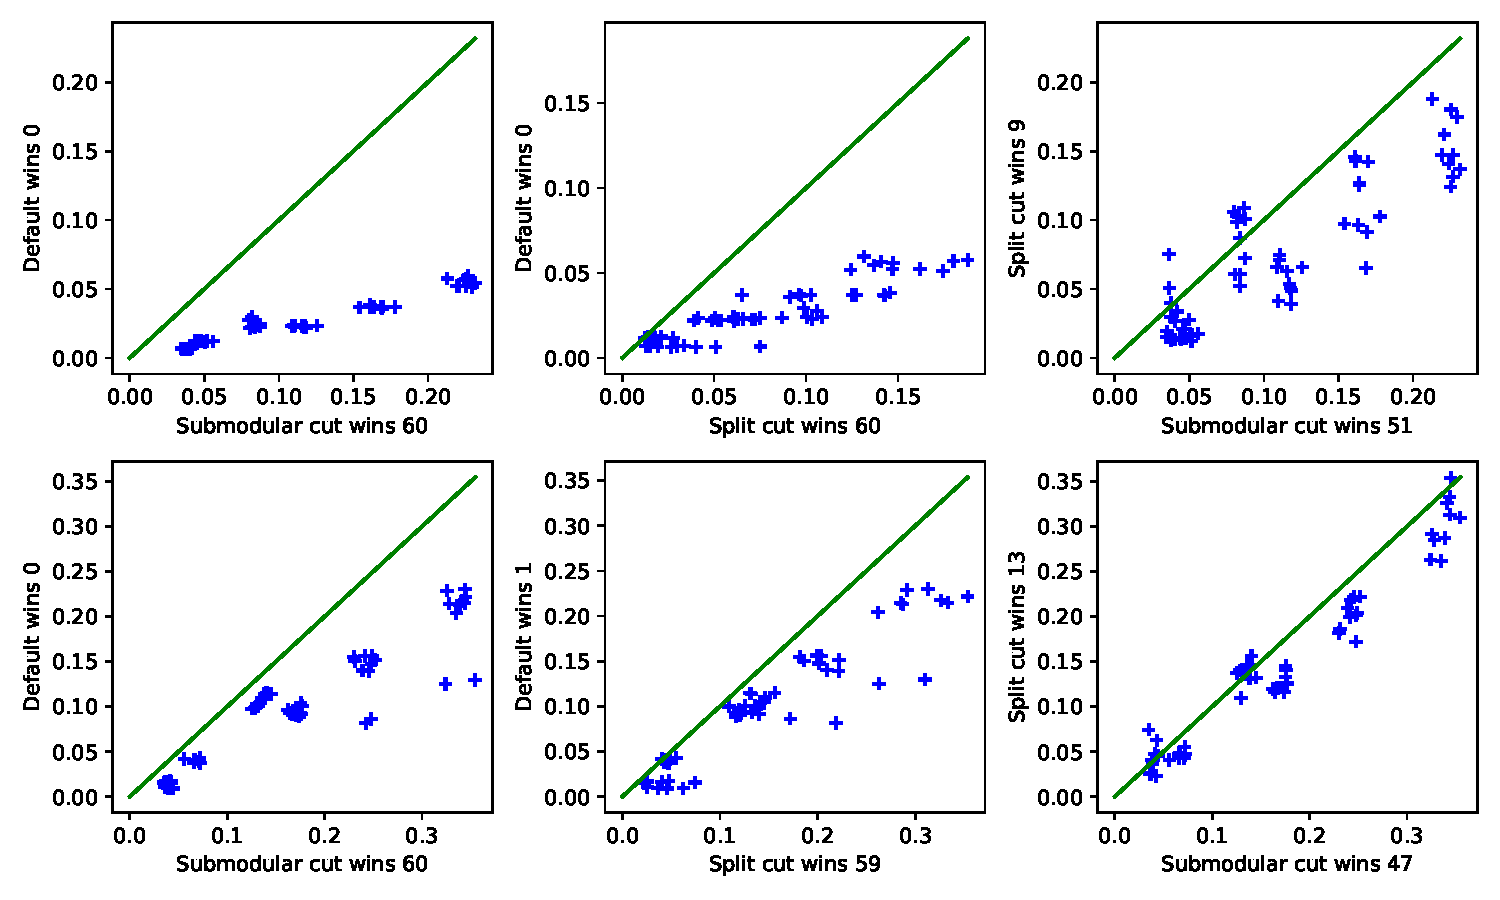
\includegraphics[width=0.99\textwidth]{Chaptersub/media/scatter_qubo.pdf}
    \caption{Scatter plots of \maxcut results in standalone (top) and embedded (bottom) configurations}
    \label{fig:qubo}
\end{figure}

%\bigskip

\noindent\textbf{Experiment 2:} \pbm.
As  mentioned, \pbm is a MUBO problem, a generalization of QUBO. We can use techniques from \Cref{sec.ss} to generate intersection cuts.   


POLIP \cite{Ulriks} is a library of polynomially constrained
mixed-integer programming instances. All MUBO instances in  POLIP with degree higher than 2 are 41 ``autocorr\_bern'' instances,  which are also included in MINLPLib \cite{minlplib,Vigerske2022Feb}.
These instances arise from short ranged non-disordered lattice spin model (the Bernasconi model) \cite{liers2010non} in theoretical physics. The problem is to determine a ground state in the Bernasconi model  minimizing a degree-four energy polynomial: $\frac{n}{n-r+1}\sum_{i = 0}^{n-r} \frac{1}{r(r-1)} \sum_{d =1}^{r-1}(\sum_{j = i}^{i+r-1-d} z_j z_{j+d})^2$, where $z \in \{-1,1\}^n$. The number $n$ of variables in these instances is chosen from 20 to 60, and the interaction range $r$ is chosen from 3 to 6. The problem is reformulated into a degree-4 BMP with $m = 0$ in MINLPLib through the transformation $z_j = 2x_j -1$.  \scip  constructs the extended formulation \eqref{ref.dopt}. We use the best-known primal bound from MINLPLib as the reference primal bound.  

In \Cref{beta}, we report the computational results. For the standalone (resp. the embedded) configuration, the relative improvement of submodular cuts is $504\%$  compared to $117\%$   of split cuts. As indicated by the scatter plots in \Cref{fig:mubo}, the submodular cut setting outperforms the split cut setting in 29 instances under the standalone configuration. Regarding the embedded configuration,  the relative improvement of submodular cuts is $98\%$,  compared to $49\%$   of split cuts.  As indicated by the scatter plots, the submodular cut setting wins in 31 more instances than the  spit cut setting under this configuration.


In both configurations, the submodular cuts are better than the split cuts in terms of the closed root gap. Moreover, under the embedded configuration, the difference in the relative improvements between submodular cuts and split cuts  is  $48\%$. This is larger than $28\%$ of \maxcut benchmark under the same configuration. This divergence between degree-2 and degree-4 MUBO suggests that the submodular cuts are suitable for high-order Boolean multilinear constraints.

We recall that to solve the nonlinear equations, the hybrid discrete Newton algorithm needs oracle access to the value of the Boolean multilinear function. For some instances, a Boolean multilinear function may consist of thousands of multilinear terms. After  a code timing analysis, we find that the  separation of submodular cuts spends the most  time computing the function value. Therefore, this is the main time performance bottleneck, which needs to be  optimized in the future. In accordance with \maxcut results,  non-maximal $\cS$-free sets may yield stronger cuts. Thus, the geometrical relation between the $\cS$-free sets and the optimal tableau cone matters.

In \Cref{sec.appb}, we conduct a branch-and-bound test.
\begin{table} [htbp]
\centering
\scalebox{0.85}{
\begin{tabular}{c|cr|cccr|cccr}
\toprule
\multirow{2}{*}{\texttt{Configuration}} &
\multicolumn{2}{c|}{\texttt{Default}}    &
\multicolumn{4}{c|}{\texttt{Submodular cut}} &
\multicolumn{4}{c}{\texttt{Split cut}} 	 \\
 & closed & time & closed & relative & time & cuts & closed & relative & time & cuts\\
\hline
standalone & 0.008 & 8.46 &  0.053 & 6.039 & 28.03 & 68.83 & 0.032 & 2.170 & 10.56 & 20.48 \\
embedded&  0.051 &  13.60  &  0.079 & 1.979 & 46.20 & 28.20 &  0.067 & 1.491 & 20.43 & 9.43 \\
\bottomrule
\end{tabular}}
\caption{Summary of  \pbm results}\label{beta}
\end{table}


\begin{figure}[h]
    \centering
    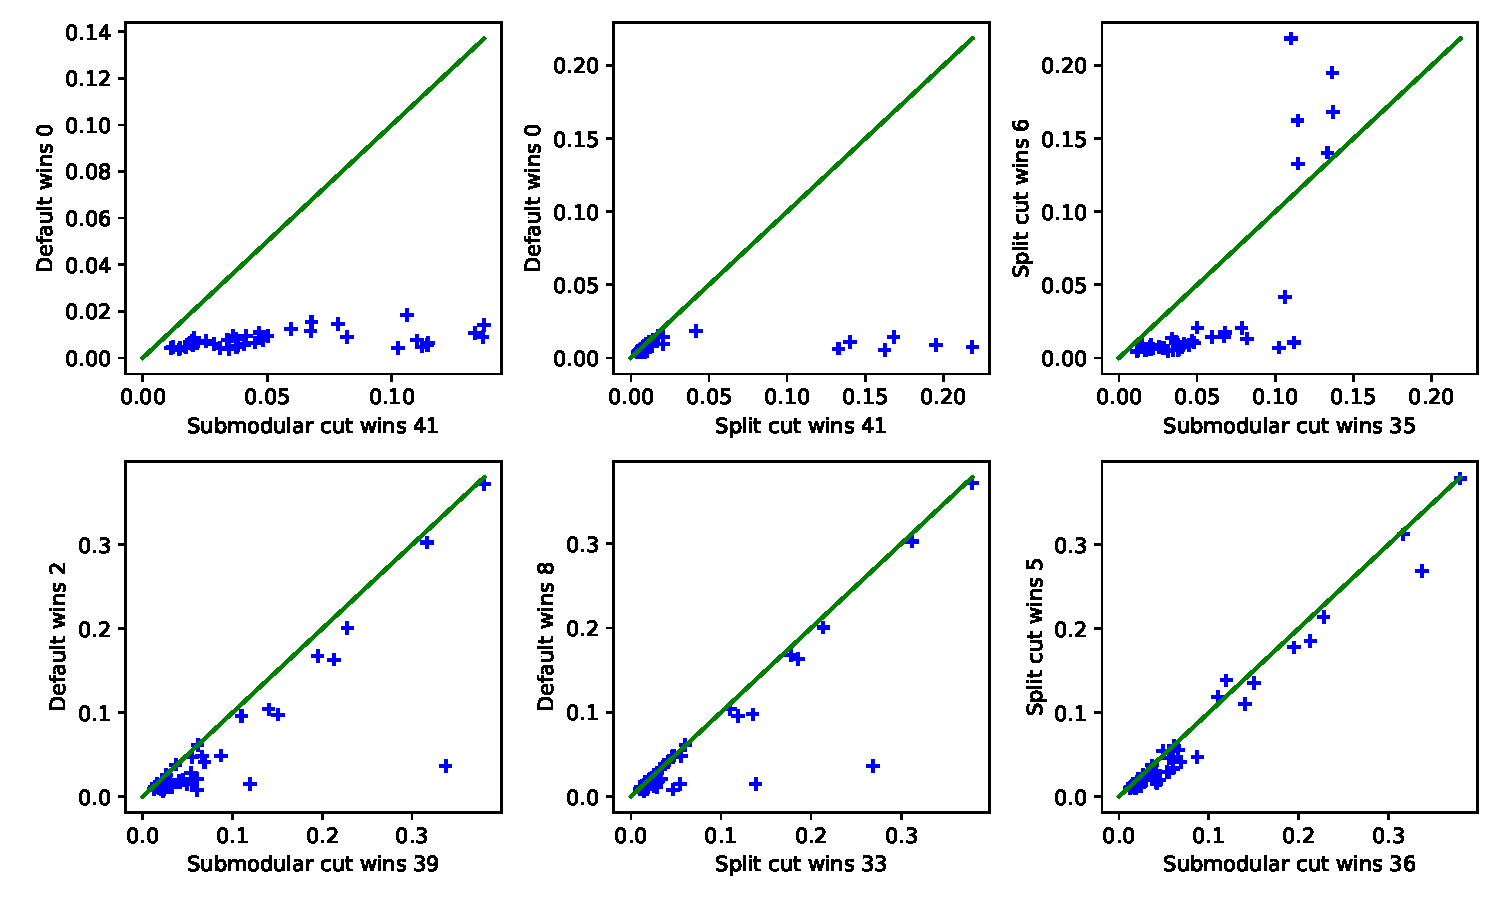
\includegraphics[width=0.99\textwidth]{Chaptersub/media/scatter_mubo.pdf}
    \caption{Scatter plots of \pbm results in standalone (top) and embedded (bottom) configurations}
    \label{fig:mubo}
\end{figure}

\textbf{Experiment 3:} \bdopt.
As mentioned before, the \bdopt problem has a submodular maximization form \eqref{eq.optimal2}. In particular, we can encode it as an extended formulation \eqref{ref.dopt} in \scip. \scip generates gradient cuts for this convex MINLP. Therefore, we can obtain LP relaxations and simplicial conic relaxations.

 Our benchmark consists of two sub-benchmarks.  Recall that the binary vector $x$ selects a subset of $\{M_j \t{M_j}  \in \bS^m\}_{j \in [n]}$, and the information matrix $M(x)$ in \eqref{eq.optimal2} is the sum of matrices in the selected subset. Thus, the problem data of \eqref{eq.optimal2} are variable dimension $n$, matrix size $m$, cardinality number $k$, and matrices $M_j \t{M_j}$.  We next outline the procedure for generating them.
 
The first sub-benchmark consists of 15 block design  instances. We follow the method in \cite{sagnol2015computing} to generate these instances.  Let $x:=(x_{1,2},x_{1,3},\dots,x_{1,m+1},\dots,x_{m,m+1}) \in \{0,1\}^n$, where $n =\binom {m+1} 2$. Let  $H(x)$  be an undirected graph  with $m+1$ vertices. If $x_{i,i'} =1$, there is an edge between vertices $i,i'$; otherwise, no edge 
connects them. We have $M(x) = P L(x)\t P$, where $L(x) := \sum_{i,i'} x_{i,i'} (\mathbf{1}_i - \mathbf{1}_{i'} ){(\mathbf{1}_i - \mathbf{1}_{i'})} ^{\top} \in \bS^m \subseteq \bR^{m \times m}$ is
the Laplacian of $H(x)$, and $P \in \bR^{m \times (m+1)}$ is the matrix
that transforms an $(m+1)$-dimensional vector $v$ to the vector obtained by keeping the first
$m$ entries of $v$.  In other words, $M(x)$ is the submatrix of the Laplacian of $H(x)$
obtained by removing its last row and last column. Then an optimal solution to \eqref{eq.optimal} corresponds to the graphs with $n$ nodes and $k$
edges that have a maximum number of spanning trees. Note that  $M_j =  P  (\mathbf{1}_i - \mathbf{1}_{i'} )\in \bR^{m \times 1}$ is a single-column matrix, which  is degenerated to a $m$-dimensional vector.  We generate a block design instance for each combination of $m \in \{10, 11, 12\}, n =\binom {m+1} 2, k \in \{m, m+1, m+2, m+3, m+4\}$. This results in a total of 15 combinations.

The second sub-benchmark consists of 30 random Gaussian instances. We generate a Guassian instance for each combination of \[(n,m) \in \{(50,20),(50,30),(60,24),(60,36),(70,28),(70,42)\}\] and \[k \in \{m,m+1,m+2,m+3,m+4\}.\] This results in a total of 30 combinations. We still let each $M_j$ be a single-column matrix (\ie a vector), and its entries  are drawn from a Gaussian distribution with zero mean  and  a variance of $1/\sqrt{n}$. 



We set the regularization constant $\epsilon $ to $10^{-6}$. \scip can find  primal feasible solutions at the root node using its internal heuristics. We select the best primal bound given by these solutions among all settings as the reference primal bound.  Since \scip's internal gradient cuts are important for linearizing convex nonlinear constraints, we  keep the gradient cuts but disable all integer-oriented cuts (GMI cuts and mixed-integer rounding cuts etc.) in the standalone configuration.

In \Cref{gamma}, we report the computational results. We divide the results of block design and Gaussian random instances, since the density of  matrices are different. Looking at the default setting in different benchmarks, there is  no difference between the standalone and embedded configurations in terms of the closed root gap. This means that integer-oriented cuts do not improve the root node LP relaxations. We see the same problem for intersection cuts, which do not close the root gap but increase the computing time.  In particular, the number of separated cuts is around one. Thereby, many intersection cuts are too weak to add to the cut pool.

We recall that  intersection cuts and many integer-oriented cuts are LP-based cuts, \ie derived from an LP relaxation of  the extended formulation \eqref{ref.dopt}. Therefore, their strengths depend on the LP relaxation.  Based on the types of MINLPs, there are two basic ways to construct initial LP relaxations.  For nonconvex MINLPs, one way usually uses the factorable programming and term-wise envelopes \cite{mccormick1976computability}. Notable examples are Boolean multilinear constraints and  continuous quadratic constraints \cite{munoz2020maximal}.  The McCormick envelopes or Boolean linearization techniques are used to construct their LP relaxations, which have a finite number of constraints.  


For convex MINLPs, the other way linearizes nonlinear constraints, and the number of constraints in the LP relaxation can grow to infinity. This is because  a convex nonlinear constraint is equivalent to an infinite number of linear constraints.  Given that \scip may incorporate numerous gradient cuts to approximate the convex MINLP \eqref{ref.dopt}, we can better understand its behavior in a simplified scenario. Consider a smooth convex body approximated by a polyhedral outer approximation, where each vertex and its associated faces define one or several simplicial cones, representing optimal tableau cones. As the polyhedron closely approximates the convex body, the vertex comes closer to the border manifold of the convex body, and the simplicial cones approach the tangent space of the manifold at that vertex. Consequently, the cones become very flat, and in the most extreme case, they turns into a hyperplane defining the tangent space. When a hyperplane intersects an $\cS$-free set, this results in the hyperplane itself. Therefore, it is highly likely that our separators will generate weak intersection cuts. In summary, the weakness of intersection cuts is due to the flatness of the optimal tableau cone.

\begin{table} [htbp]
\centering
\scalebox{0.71}{
\begin{tabular}{c|c|cr|cccr|cccr}
\toprule
\multirow{2}{*}{\texttt{Benchmark}} & \multirow{2}{*}{\texttt{Configuration}} &
\multicolumn{2}{c|}{\texttt{Default}}    &
\multicolumn{4}{c|}{\texttt{Submodular cut}} &
\multicolumn{4}{c}{\texttt{Split cut}} 	 \\
 & & closed & time & closed & relative & time & cuts & closed & relative & time & cuts\\
\hline
 \multirow{2}{*}{\texttt{Block design}} & standalone &  0.59 & 20.46 & 0.59 & 1.0 & 18.71 & 1.84 & 0.59 & 1.0 & 11.62 & 1.77  \\
  &  embedded & 0.59 & 21.44 & 0.59 & 1.0 & 19.0 & 1.84 & 0.59 & 1.0 & 12.41 & 1.77 \\
  \hline
 \multirow{2}{*}{\texttt{Gaussian}}  &  standalone  &  0.83 & 213.13 & 0.83 & 1.0 & 415.07 & 1.45 & 0.83 & 1.0 & 214.17 & 1.45 \\
& embedded  &  0.83 & 214.77 & 0.83 & 1.0 & 426.33 & 1.45 & 0.83 & 1.0 & 214.14 & 1.45 \\
\hline
 \multirow{2}{*}{\texttt{All}}  &  standalone  &   0.75 & 98.47 & 0.75 & 1.0 & 149.54 & 1.57 & 0.75 & 1.0 & 82.6 & 1.55 \\
& embedded  &   0.75 & 100.47 & 0.75 & 1.0 & 153.01 & 1.57 & 0.75 & 1.0 & 84.31 & 1.55 \\
\bottomrule
\end{tabular}}
\caption{Summary of  \bdopt results}\label{gamma}
\end{table}

\begin{figure}[h]
    \centering
    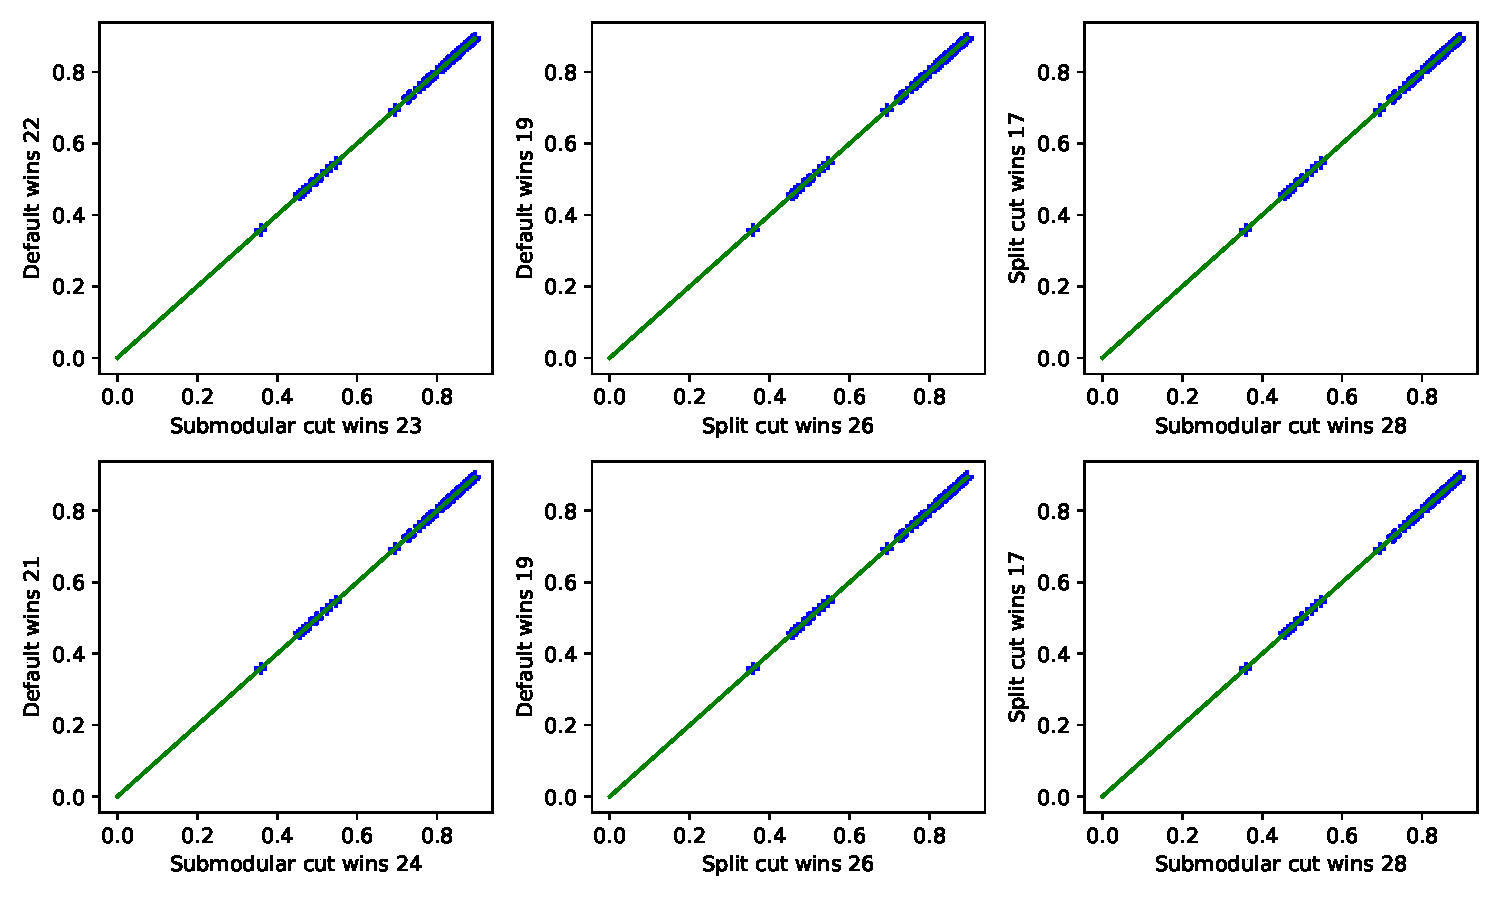
\includegraphics[width=0.99\textwidth]{Chaptersub/media/scatter_dopt.pdf}
    \caption{Scatter plots of \bdopt results in standalone (top) and embedded (bottom) configurations}
    \label{fig:dopt}
\end{figure}



\subsection{Supplementary branch-and-bound computational results}
\label{sec.appb}
We also have an additional branch-and-bound test for \maxcut problem instances in \Cref{sec.cresult}. This test was designed to assess the performance and properties of our cuts in a "production-level" environment, which presents more complex challenges compared to the root node experiment. As such, the parameter settings and analysis in this test are more intricate and require a detailed explanation, which we provide below.

We conducted our tests under the embedded configuration, where the branching rule, node selection rule, and primal heuristics adhere to \scip's defaults. We made adjustments to some parameters specifically to control the behavior of our cut separators in the branch-and-bound algorithm. These parameters are as follows:
\begin{itemize}
	\item SEPA\_FREQ:  the default frequency for separating cuts. We set it to 0, meaning that our cut separators are called at the root node.
	\item SEPA\_NCUTSLIMITROOT: the limit for the number of cuts generated  at the root node. We  set it to 60.
	\item SEPA\_MAXBOUNDDIST: the default maximal relative distance from the current node's dual bound to primal bound compared to the best node's dual bound for applying separation. We set it to 1, meaning that separation is applied at all search nodes.
\end{itemize}


Due to the substantial number of parameter combinations, tuning the parameters for the branch-and-bound test is more challenging compared to the root node experiment. For instance, \scip's internal Gomory mixed-integer cut separator \cite{BibEntry2023Jul2,cornuejols2013safety} is limited to applying at most 30 cuts at the root node, while \scip's quadratic intersection cut separator \cite{BibEntry2023Jul3,chmiela2022implementation} employs at most 20 cuts at the root node and 2 cuts at each non-root node.


In a preliminary branch-and-bound test, we find  that even the default setting can solve the ``pw'' instances of density 0.1 within 100 seconds, while all settings run 3600  seconds on the other instances. To have an unbiased result, we remove ``pw'' instances of density 0.1 and create a sub-benchmark called \maxcut-sub.


For the following branch-and-bound test, we measure the closed duality gap (abbreviated as gap), the relative improvement of the closed duality gap to the default setting, the number of search nodes (abbreviated as nodes), and the number of applied cuts.

\begin{table} [htbp]
\centering
\scalebox{0.85}{
\begin{tabular}{c|cr|cccr|cccr}
\toprule
\multirow{2}{*}{\texttt{Benchmark}} &
\multicolumn{2}{c|}{\texttt{Default}}	&
\multicolumn{4}{c|}{\texttt{Submodular cut}} &
\multicolumn{4}{c}{\texttt{Split cut}}      \\
 & gap & nodes & gap & relative & nodes & cuts & gap & relative & nodes & cuts\\
\hline
 \maxcut-sub  &  0.605 & 231372 & 0.596 & 0.981 & 220176 & 59.87 & 0.618 & 1.026 & 207078 & 42.2\\
\bottomrule
\end{tabular}}
\caption{Summary of \maxcut-sub results in the embedded branch-and-bound test}\label{Aalpha}
\end{table}

Our observations indicate that the submodular cut setting performs slightly worse than the default setting, while the split cut setting performs marginally better than the default setting. As shown in \Cref{fig:qubo3}, the difference in closed duality gaps between the submodular/split cut and default settings is no more than 2\%.
This shows that the optimization landscape of \maxcut problems is very complicated. As for our parameter settings, intersection cuts cannot have a significant impact on the branch-and-bound algorithm.




In contrast to the results in the root node experiment, we find that the split cut setting outperforms the submodular cut setting in the branch-and-bound test. Detailed cut information obtained during debugging reveals that the condition number of submodular cuts can be thousands of times larger than that of split cuts, and the submodular cuts can be denser as well. Consequently, these numerical properties make the submodular cuts less stable and efficient compared to the split cuts.

When considering the approximation of the Boolean-hypograph $\hyp_{\cB}(g)$, where $g$ represents any function over $\cB$, we can deduce from \Cref{thm.bin} that the splits define a class of maximal Boolean-hypograph-free sets. Although the split cuts are independent of  the values of $g$,  we can use the split cuts to approximate the Boolean-hypograph of $g$.  While one can find other Boolean-hypograph-free sets based on the values of $g$, the resulting cuts will likely exhibit the same numerical properties as our submodular cuts.

As a result, future research should consider this finding when exploring intersection cuts. However, it is also worthwhile to investigate the performance of submodular cuts in other problems and algorithms, such as \pbm problems and the diving heuristic.






\begin{figure}[h]
    \centering
    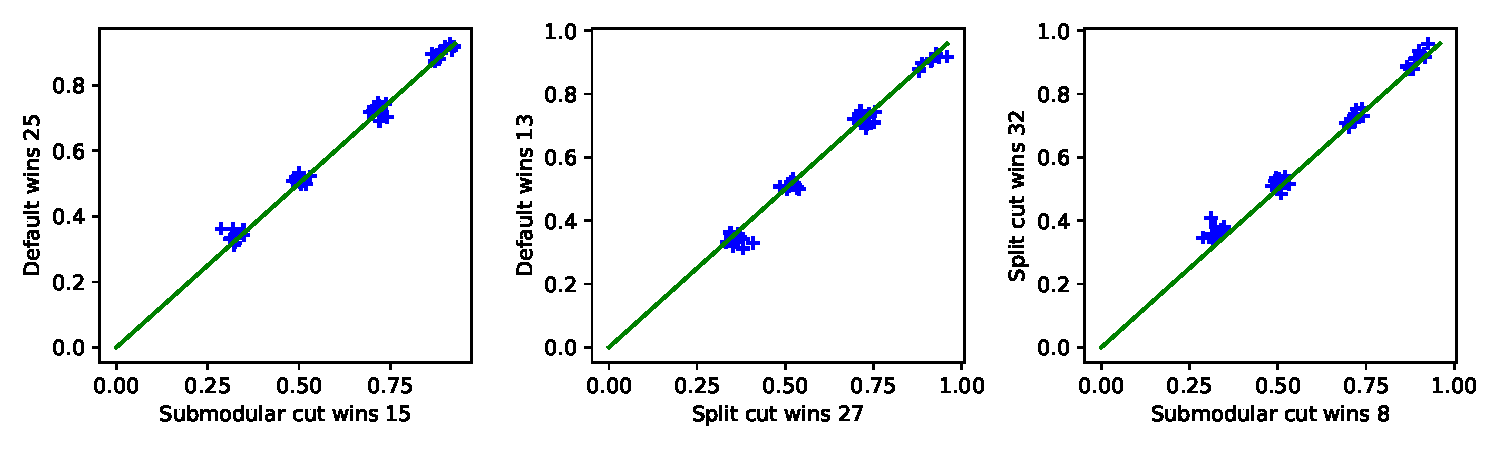
\includegraphics[width=0.99\textwidth]{Chaptersub/media/scatter_qubo_bc.pdf}
    \caption{Scatter of \maxcut-sub results in the embedded branch-and-bound test}
    \label{fig:qubo3}
\end{figure}

\section{Conclusion}\label{sec13}

We construct Boolean-hypograph-free sets for  submodular functions. Our construction relies on a new continuous extension of submodular functions. We characterize maximal Boolean-hypograph-free sets, and generalize our results to sets involving submodular-supermodular functions. These yield intersection cuts for Boolean multilinear constraints. We exploit the submodular structure in an extended formulation of the \dopt problem. We propose a hybrid discrete Newton algorithm that can compute intersection cuts efficiently and exactly. The computational results show that intersection cuts derived from the submodularity are better than those derived from  split cuts for \maxcut and \pbm problems in the root-node experiments. For convex MINLPs, our computational results on the \bdopt problem suggest that  simplicial conic relaxations given by  gradient cuts can be flat, which makes intersection cuts weak.

%As for future studies, an open question is how to extend our methods for discrete submodular functions on general lattices \cite{bach2019submodular} or constrained DR submodular functions \cite{yu2022constrained}. This will result in intersection cuts for integer multilinear constraints  or other discrete nonconvex sets. Another direction is to study the maximal Boolean-hypograph-free sets that enlarge the extended envelope epigraph $\ee{f}$. This study may require additional structural information on submodular functions. We recall that the lifting procedure \cite{ahmed2011maximizing,shi2022sequence} for the base inequalities \cite{Nemhauser1988} only exists for a special class of submodular functions.
%Therefore,  one may only construct  maximal Boolean-hypograph-free sets enlarging $\ee{f}$ for  some special class of submodular functions. This may lead future studies to concrete examples with additional structures, unlike the general submodular function studied in this chapter. A possible strengthening of intersection cuts can use the monoidal technique \cite{ChmielaMunozSerrano2023} or the negative ray extension \cite{chmiela2022implementation}. Constructing intersection cuts from a non-polyhedral corner relaxation is an important open question for convex MINLPs.



%%===========================================================================================%%
%% If you are submitting to one of the Nature Portfolio journals, using the eJP submission   %%
%% system, please include the references within the manuscript file itself. You may do this  %%
%% by copying the reference list from your .bbl file, paste it into the main manuscript .tex %%
%% file, and delete the associated \verb+\bibliography+ commands.                   		 %%
%%===========================================================================================%%



\chapter{Branch-and-price for submodular bin packing}
\label{chap.sbp}



\section{Introduction}

Bin packing (BP) is an important combinatorial optimization problem with applications in various fields, including call centers, healthcare, container shipping, and cloud computing. These applications are typically modeled as BP problems that aim to pack unsplittable items into a minimum number of bins, with a capacity constraint on each bin.  Formally, a BP problem can be written as the following Binary Linear Programming (BIP) problem:
 \begin{subequations}
 \label{bp}
 \begin{align}
 \min \quad \sum_{j \in \cM} {y}_{{j}}, \qquad&\\
 \st \qquad \sum_{i \in \cN} \mu_i v_{ij} \le c {y}_{{j}}, \qquad& \forall j \in \cM, \label{bp.cap} \\
  \sum_{j \in \cM} v_{ij} = 1, \qquad& \forall i \in \cN, \label{bp.cover} \\
  v_{ij} \in \{0,1\}, \qquad& \forall i \in \cN, j \in \cM, \label{bp.x}\\
  y_{j} \in \{0,1\}, \qquad& \forall j \in \cM \label{bp.y},
 \end{align}
 \end{subequations}
where  $\cM:=\{1,\cdots,m\}$ is the index set of potential bins ($m$ is the number of potential bins), $\cN:=\{1,\cdots, n\}$ is the index set of items ($n$ is the number of items),  $c$ is the capacity which is the same for every bin, and $\mu_i$ is the size of item $i$.  Variable $y_j$ decides whether bin $j$ is used, and variable $v_{ij}$ indicates whether item $i$ is allocated to bin $j$.  Capacity constraints \eqref{bp.cap} stipulate that the capacities of bins are not exceeded, and set partition constraints \eqref{bp.cover} require that each item is exactly allocated to one bin.


 In many practical applications of BP, nominal item sizes $\mu$ are not revealed before the allocation decision is made, so uncertainty arises.    Probabilistic modeling of  capacity constraints \eqref{bp.cap} allows item sizes $\mu$ to be random parameters, and thus the uncertainty is taken as a probability distribution on $\mu$. We consider  two  commonly used probabilistic BP models.  The first probabilistic model is the BP with chance constraints (BPCC) \citep{song2014chance}. By assuming item sizes $\mu$ following a given (multivariate) probability distribution, BPCC requires that each capacity constraint in \eqref{bp.cap} should be respected with a probability at least $\alpha$, written as the following chance constraints \citep{charnes}:
\begin{equation}
 \label{eq.chance}
      \quad \bP(\sum_{i \in \cN} \mu_i v_{ij} \le c{y}_{{j}}) \ge \alpha, \qquad \forall j \in \cM.
	 \end{equation}
 The second probabilistic model is the distributionally robust BP (DRBP) \citep{zhang2020branch,cohen2019overcommitment}. It models the worst case of chance constraints \citep{ghaoui2003}. More specifically, given a family $ \mathscr{D}$ of probability distributions  of $\mu$, DRBP requires that each chance constraint in \eqref{eq.chance} should be respected for any probability distribution within $ \mathscr{D}$. Thereby, capacity constraints of DRBP can be formulated as the following distributionally robust constraints
 \begin{equation}
 \label{eq.chance2}
    \inf_{\mu \sim \mathscr{D}} \bP(\sum_{i \in \cN} \mu_i v_{ij} \le c{y}_{{i}}) \ge \alpha,  \qquad \forall j \in \cM.
 \end{equation}
 
 Computational optimization of BPCC and DRBP models is challenging due to probabilistic constraints.  Stochastic optimization methods can tackle mathematical optimization problems with probabilistic constraints. The sample average approximation (SAA) is a common stochastic optimization method for  chance-constrained and distributionally robust optimization problems \citep{luedtke2008sample, bertsimas2018robust}. It approximates these problems as  two/multi-stage MILP problems and computes approximate solutions that converge to an optimal solution in a probabilistic sense. Previous works, such as \cite{zhang2020branch, denton2010optimal,batun2011operating}, apply tailored SAA methods to solve BPCC and DRBP.
 
 Several recent works show that, under various assumptions on probabilistic distributions, BPCC and DRBP are equivalent to or well-approximated by a  deterministic optimization problem, namely, submodular BP (SMBP). It is shown in \cite{cohen2019overcommitment} that, BPCC has an SMBP formulation,   if item sizes $\mu$ follow independent Gaussian distributions;   SMBP also provides an upper bound for BPCC with item sizes $\mu$ under general independent distributions over bounded intervals (we note that then SMBP becomes a restriction of BPCC, and thus its solution is always feasible to BPCC.). It is shown in \cite{zhang2018ambiguous} that DRBP has an SMBP formulation, if distributions in $\mathscr{D}$ have the same mean values and the same diagonal covariance matrix.
 
 Given the applicability of the previous assumptions, SMBP is an appealing alternative formulation to BPCC and DRBP, as it can be solved optimally in a finite time, while  the convergence rate of  SAA methods for BPCC and DRBP depends on the number of samples.  SMBP already finds its applications in  cloud computing \citep{cohen2019overcommitment}, surgery planning \citep{deng2019chance}, and operating room planning \citep{wang2021chance}. The environment is highly dynamic for these applications, and uncertainty plays a significant role in practical models. These applications give rise to a need for efficient algorithms to solve SMBP.

 In this chapter, we study the exact algorithms for solving SMBP. SMBP has the following Binary Nonlinear Programming formulation:

 \begin{subequations}
 \label{master.submod}
 \begin{align}
 \min \quad \sum_{j \in \cM} {y}_{{j}}, \qquad&\\
 \st \qquad \sum_{i \in \cN} a_i v_{ij} + \sigma\sqrt{\sum_{i \in \cN} b_i v_{ij} } \le c {y}_{{j}}, \qquad& \forall j \in \cM, \label{master.submod.cap} \\
  \sum_{j \in \cM} v_{ij} = 1, \qquad& \forall i \in \cN, \label{master.submod.cover} \\
  v_{ij} \in \{0,1\}, \qquad& \forall i \in \cN, j \in \cM, \label{master.submod.x}\\
  y_{j} \in \{0,1\}, \qquad& \forall j \in \cM \label{master.submod.y}
 \end{align}
 \end{subequations}
where $a_i,b_i$ are parameters inferred from the distribution of $\mu_i$. This formulation is a compact nonlinear version of \eqref{bp}. We remark that the left-hand side of the constraint \eqref{master.submod.cap} is a submodular function over $x$ \citep{atamturk2008polymatroids}, so SMBP is named after this function. A constraint in the form of \eqref{master.submod.cap} with $y_j$ fixed to 1 is called a submodular knapsack constraint.


To solve SMBP, the state-of-art exact algorithm uses general-purpose integer-programming solvers to solve its Binary Second-Order Conic Programming (BSOCP) reformulation \citep{zhang2018ambiguous}, which valid inequalities can further strengthen \cite{atamturk2008polymatroids}. The experiment  in \cite{zhang2018ambiguous} shows that small instances with item number $n$ up to $40$ and bin numbers $m$ up to 10  can be solved to optimality by this exact algorithm.

The intuition underlying this chapter is that the  decomposition is a promising approach to tackling large-scale classical BPs: a BP is reformulated into a set cover formulation based on enumerating all feasible packing patterns; then its continuous relaxation is solved using a column generation approach \citep{gilmore1961linear}. The branch-and-price algorithm integrates column generation with the branch-and-bound algorithm. It is the state-of-the-art exact algorithm for solving DW decomposition of classical BPs \citep{wei2020new, delorme2016bin}.


We propose the first DW decomposition and set cover formulation for SMBP, and design a branch-and-price algorithm with tailored methods for solving pricing problems. After our DW decomposition of SMBP,   the nonlinearity moves to the pricing submodular knapsack subproblem, which has a linear objective function and a submodular capacity constraint. One can avoid the growing number of nonlinear constraints \eqref{master.submod.cap} in the compact formulation \eqref{master.submod}, when solving larger instances.

The DW decomposition provides a skeleton of our main algorithm. The techniques for solving general DW decomposition problems  are vast, to name a few, we refer to \cite{frangioni2013stabilized} for stabilization techniques,  \cite{coniglio2019lexicographic} for lexicographic pricing, \cite{wei2020branch} for goal cuts and early termination, and \cite{jepsen2008subset} for non-robust cuts. 
In \cite{pessoa2021solving}, a simple parameterization enables the use of several  advanced techniques in the  branch-cut-and-price VRPsolver \cite{pessoa2020generic}: automatic stabilization
by smoothing \cite{pessoa2018automation}, limited-memory rank-1 cuts \cite{pecin2017improved}, enumeration, hierarchical strong branching over accumulated resources \cite{gelinas1995new}, and
limited discrepancy search diving heuristics.
In this chapter, we focus on algorithmic innovation that exploits the specific nonlinear structure of pricing problems and new techniques to speed  up the convergence of column generation.


 As the study in \cite{zhang2018ambiguous} for the compact formulation, the nonlinearity is a crucial feature for model representability, so it is unavoidable and needs a special algorithmic treatment. In our case, pricing problems have submodular knapsack constraints involving nonlinear functions. We give two different views of nonlinearity. First, we can represent the submodular knapsack constraint via second-order constraints, which many general solvers then accept. Alternatively, we propose a non-convex Mixed-Binary Quadratically Constrained Programming (MBQCP) formulation for the submodular knapsack. A PWL  function is linear in each partition of its domain and can be modeled by a MILP formulation \citep{vielma2010}. PWL functions have been used to approximate or relax non-convex MINL) problems \citep{geissler2012using}.  Despite its non-convexity, the critical feature of the MBQCP formulation is that its only nonlinear function is a univariate quadratic function, which is easy to approximate using a PWL function. We construct the PWL relaxation for the submodular knapsack and combine it with cutting planes to form an exact PWL relaxation-based branch-and-cut (PWL-B$\&$C) algorithm.

 The submodular knapsack  is essential as it models the chance-constrained knapsack problem \citep{goyal2010ptas}. We thus provide an approach for solving submodular knapsack problems different  from the pure valid inequality approach in \cite{atamturk2008polymatroids,atamturk2009submodular}.
 
 We propose  several strategies to accelerate the convergence of the branch-and-price algorithm, i.e., improve primal and dual bounds. The Farley bound \cite{farley1990note,vance1994solving}  is an early valid dual bound before the termination of the column generation procedure \cite{wei2020new, gleixner2020price}.
The formula for the Farley bound imposes a condition on whether an exact pricing algorithm can improve the current dual bound. If the condition is not satisfied, the exact pricing algorithm is unnecessary, so we can use fast pricing heuristic. Our branch-and-price algorithms use a hybrid pricing strategy to speed up the column generation procedure. The hybrid pricing strategy is thus an intermediate between exact pricing and heuristic pricing strategies \cite{blanco2023branch}.
 
 There are few publicly available instances of SMBP problems. In \cite{cohen2019overcommitment}, there is a method to generate instances from BPCC and DRBP under various distributions. We generate instances of three different scales  by this method and conduct computational experiments on them. We implement our branch-and-price algorithm for the set cover formulation of SMBP and find that it outperforms existing methods, which solve the compact BSOCP formulation \cite{zhang2018ambiguous}. Our core innovation,  PWL-B$\&$C pricing algorithm, and hybrid pricing strategy, significantly improve the branch-and-price algorithm.
 





\subsection{Literature review}
As mentioned, there are several steps of transformation from BP with uncertainty to SMBP. We review these transformations and algorithms for solving associated transformed models.

The surgery planning problem is a typical application of BP with uncertainty in healthcare, where the surgery duration (item size) is assumed to be stochastic. Some pioneering works
 \citep{ denton2010optimal, batun2011operating} allow violations to capacity constraints (the left-hand side of \eqref{bp.cap} thus can be greater than the capacity) rather than consider chance constraints.  To minimize these violations, they  use a penalty approach by adding the expectation of the sum of these violations into the objective function. Therefore, the transformed BP model is a standard stochastic optimization problem called stochastic BP (SBP). SBP can be further modeled and solved as a stochastic two-stage mixed-integer programming problem: the first stage variables are the bin variables $y$, the second stage variables are the item variables $v$, and the expected violation is the second stage objective.  In some works \citep{cardoen2010operating, deng2020}, only the expected penalty is considered in the models.
 
 
 
 Compared to SBP, BPCC, and DRBP can control the violation of each capacity constraint with  a guaranteed probability bound, and thus they are more accurate models for BP with uncertainty. To solve BPCC and DRBP, there are approximation algorithms  and exact algorithms. (Sampling-based) approximation algorithms usually converge  asymptotically to an optimal solution when the sampling number increases (as SAA methods), and exact algorithms usually converge in  finite time. However, exact algorithms are mostly available for deterministic optimization problems.
 
 In \cite{shylo2013}, a variant of  BPCC in surgery planning is studied:   items (surgeries) are allocated to  a  given set of bins (time blocks), the goal is to minimize the sum of expected capacity residuals (undertime), subject to chance constraints for overuse of  bins' capacities (overtime). Assuming that the operation duration follows a multivariate normal distribution, the authors reformulate the problem as a deterministic optimization problem containing a convex objective and submodular capacity constraints. In \cite{song2014chance}, a special BPCC with the probability distribution over finite support is studied. It has  a BIP formulation, which an exact algorithm can solve.  As mentioned before, for various probabilistic distributions \cite{cohen2019overcommitment,zhang2018ambiguous},  BPCC and DRBP admit a deterministic SMBP reformulation, which can be solved by exact algorithms.
 
 
Regarding solution algorithms, an SAA-based   algorithm \cite{zhang2020branch} can solve BPCC approximately, whose scenario subproblem is solved exactly by a DW decomposition approach. In addition, SMBP reformulation of DRBP  \cite{zhang2020branch} can be approximated by a MILP, which is solved by a DW decomposition approach. The only tailored exact algorithm for BPCC and DRBP  \cite{zhang2018ambiguous} solves their compact SMBP reformulations. As for the deterministic variant of BPCC, the authors of   \cite{shylo2013} propose an exact outer approximation algorithm enhanced with PWL relaxation of submodular knapsack constraints, and the algorithm is a multi-search tree method, i.e., an underlying MILP solver will be called multiple times. In conclusion, no exact algorithm based on DW decomposition exists to solve SMBP. Meanwhile, DW decomposition is  already used for various approximated problems.


This exception  may be due to the lack of efficient exact algorithms to solve submodular knapsack problems.
We note that in \cite{zhang2020branch}, DW decomposition is \textit{de facto} applied to a MILP problem, and thus the  pricing problems are also MILPs such as classical knapsack problems \citep{cacchiani2022knapsack}, which can be solved efficiently by general-purpose integer programming solvers.  The efficiency of general solvers is mostly due to the lifted cover inequalities, which are strong valid inequalities for knapsack polytope and can be constructed via sequence-independent lifting \citep{gu1999lifted}. However, for submodular knapsack, the computation of lifted cover inequalities is not tractable  \citep{atamturk2009submodular}. As we know from the literature,  the tailored algorithm can be much better than general solvers for many variants of classical knapsack, because these algorithms can exploit more problem structures than general solvers. To name a few, we refer  to the quadratic knapsack \citep{caprara1999, furini2019theoretical}, the multidimensional knapsack \citep{Puchinger2010}, and the quadratic multi-knapsack \citep{Bergman19, olivir2021}.  

 
Although general solvers are almost as complex as a black box for users, we can at least understand how they solve the submodular knapsack. The submodular knapsack can be reformulated as a BSOCP problem, which is an acceptable formulation to  \texttt{CPLEX} \citep{bliek1u2014solving} and \texttt{SCIP} \citep{berthold2012extending}. These solvers implement  LP outer approximation-based branch-and-cut (LP-B$\&$C) algorithm \citep{coey2018outer} to solve the BSOCP or general Mixed-Integer Second-Order Conic Programming (MISOCP) problems. The LP outer approximation is sometimes called the polyhedral outer approximation (or polyhedral relaxation).  In fact, any second-order conic program (SOCP) is polynomially reducible to a linear program \cite{ben2001polyhedral}. As for a submodular knapsack constraint, general solvers will linearize it into an intersection of a set of classical knapsack constraints, thus, inefficiency arises if too many linearizations are applied.


On the other hand, there are alternative exact approaches to solve some classes of nonconvex MINLPs using PWL relaxations  \citep{d2012algorithmic, geissler2012using}. For example, \cite{d2012algorithmic} obtains a convex MINLP relaxation for nonconvex MINLPs with separable nonconvex functions. The authors distinguish between convex and concave parts and then convexify the concave parts by PWL functions.


Regarding the submodular knapsack, its BSOCP (a convex MINLP) formulation has a nonlinear function over all the problem variables, which is difficult to approximate when  the dimension is high. On the other hand,  the nonconvex MBQCP formulation, where the only nonlinear function is a univariate quadratic function on a slack variable. The resulting PWL relaxation in the experiment is stronger than pure polyhedral relaxation. In our case, we will show that the quadratic function can be approximated in a ``dimension-free" way, since the nonlinearity is concentrated on a single variable. \cite{shylo2013} only uses  PWL relaxations to approximate the submodular knapsack. It requires refining PWL relaxations to achieve convergence, so their multi-search tree algorithm needs to restart the MILP solver from scratch in each iteration. In contrast, we prefix PWL relaxations and use cutting planes to achieve convergence. Therefore, our  single-search tree does not need to restart the MILP solver.



 We look at the recent development of DW decomposition and  branch-and-price algorithm for solving MINLPs
 (see \cite{allman2021branch}), such as recursive circle packing (RCP) problems  \citep{gleixner2020price}, binary quadratic problems \citep{ceselli2022dantzig}, and facility location with general nonlinear facility cost functions \citep{ni2021branch}.  There may be several ways to divide a MINLP into master and subproblems, so a MINLP may admit different DW decompositions. In \cite{ceselli2022dantzig}, the authors study the strengths of different DW decompositions for binary quadratic problems. In most cases, after applying the DW decomposition to the compact MINLP formulation, the master problem is a MILP, and the pricing problems are MINLPs.  Since pricing problems are solved in thousands of iterations, \cite{gleixner2020price} shows that any improvement in the pricing algorithm can speed up the convergence of column generation.






\subsection{Contribution}

In summary, our contribution in this chapter is threefold. As far as we know, the previous work applies DW decomposition for an approximated MILP for SMBP, and thus nonlinearity is not considered in the solving process. So, we are the first to apply  DW decomposition for SMBP with the nonlinearity considered. Built on the basic DW decomposition and branch-and-price algorithm, we develop a new hybrid pricing strategy technique to speed up the column generation, which can avoid computationally expensive exact pricing while not worsening the dual bound.  Second, for pricing submodular knapsack problems, we  propose a new MBQCP formulation and its PWL relaxation, and design a new PWL-B$\&$C algorithm  as an alternative  exact algorithm to the conventional LP-B$\&$C algorithm, which is  based on valid inequalities. Finally, we perform computational experiments on many instances to evaluate the proposed algorithms. The computational results show that our tailored branch-and-price algorithms for DW reformulation outperform the conventional branch-and-cut algorithm for BSOCP formulation implemented in a state-of-art commercial solver; and the PWL-B$\&$C algorithm can be a standalone algorithm for submodular knapsack. The source code and benchmark are released on our project website \href{https://github.com/lidingxu/cbp}{https://github.com/lidingxu/cbp}.

\subsection{Outline of the chapter}
 This chapter is organized as follows. In \Cref{sec.prob}, we describe the set cover formulation of SMBP. In \Cref{sec.bp}, we introduce the critical components of our branch-and-price algorithm: the branching rule, column generation, dual bound computation, initial columns, and primal heuristics. In \Cref{sec.price}, focusing on solving the pricing problem, we present the pricing heuristic, reformulations of the pricing problem, PWL relaxation, the exact pricing algorithm, and the hybrid pricing strategy. In \Cref{sec.experi}, we show the computational results of the proposed algorithms for instances generated from the literature and analyze their performance. In \Cref{sec.conc}, we end this chapter with a conclusion and future research directions.




\section{Set cover formulation}
\label{sec.prob}
In this section, we propose a new set cover formulation for SMBP. The formulation is derived similarly to the DW decomposition of the classical linear BP \citep{delorme2016bin}. This formulation can be solved efficiently by a branch-and-price algorithm.

A column \(p\) is defined by a binary vector as \((d_{1p}, d_{2p}, \hdots,d_{np})\), where \(d_{ip} = 1\) if item \(i\) is contained in the column \(p\). A column is called \textit{feasible} if the combination of its items can fit into a bin, i.e., satisfies the submodular capacity constraint \eqref{master.submod.cap}. The set cover formulation is based on enumerating all feasible columns, the number of which can be exponential to the number of items.

\textbf{Set notation:}

\begin{itemize}
 \item \(\cP\): the set of all feasible columns.
\end{itemize}



\textbf{Decision variables:}
\begin{itemize}
 \item $\lambda_p = \begin{dcases} 1, & \textup{if column \(p\) is used by the solution}\\
  0, & \textup{otherwise}
 \end{dcases}$ for $p \in \cP$.
\end{itemize}



We obtain the following set cover formulation for SMBP:

 \begin{subequations}
 \label{master.dw}
 \begin{align}
 \min \quad \sum_{p \in \cP} \lambda_p, \qquad&\\
 \st \qquad \sum_{p \in \cP} d_{ip} \lambda_p \ge 1, \qquad& \forall i \in \cN, \label{master.dw.sc}\\
 \qquad \lambda_p \in \{0,1\}, \qquad & \forall p \in \cP.
 \end{align}
 \end{subequations}
The set cover constraint \eqref{master.dw.sc} specifies that each item \(i\) ($i \in \cN$) is contained in at least one bin. The set cover reformulation already finds applications in vehicle routing \cite{pecin2017improved} and unsplittable multi-commodity flows \cite{xu2022branch}.

The compact formulation \eqref{master.submod} is a MINLP, but the set cover formulation \eqref{master.dw} is a MILP. Moreover, the number of nonlinear constraints in the compact formulations equals the number of potential bins. The nonlinearity of the set cover formulation is \textit{de facto} `hidden' in the pricing subproblems, and each pricing subproblem has only one nonlinear constraint.


\begin{remark}
\label{rm.bsocp}
(Modeling of BSOCP constraints)
We give a way to obtain a BSOCP formulation of the constraint $\sum_{i \in \cN} a_i v_{ij} + \sqrt{\sum_{i \in \cN} b_i v_{ij} } \le d$, where $d = c y_i$ or $d = c$. Since $v_{ij} \in \{0,1\}$, the square root $\sqrt{\sum_{i \in \cN} b_i v_{ij} }$ equals  $\sqrt{\sum_{i \in \cN} b_i v^2_{ij} }$. Then the constraint is equivalent to a SOCP constraint $ \sqrt{\sum_{i \in \cN} b_i v^2_{ij} } \le d'$, where $d' := d - \sum_{i \in \cN} a_i v_{ij}$. Then one can further reformulate the SOCP constraint into several 3d SOCP constraints $x_1 \ge \sqrt{x_2^2 +x_3^2}$, which is  acceptable by \texttt{CPLEX} \cite{bonami2015recent}.
\end{remark}

We can  obtain a BSOCP formulation of SMBP \eqref{master.submod} through the above discussion.
When comparing two formulations, a formulation is said to be ``stronger'', if it  yields a better dual bound.  

\begin{proposition}
\label{prop.strong}
The linear relaxation of the set cover formulation \eqref{master.dw} is stronger than the continuous SOCP relaxation of the BSOCP formulation of \eqref{master.submod}.
\end{proposition}
 \begin{proof}
 Let $$F_j := \{(v_{1j},\cdots,v_{nj}, y_j) \in \{0,1\}^{n+1} : \sum_{i \in \cN} a_i v_{ij} + \sigma\sqrt{\sum_{i \in \cN} b_i v_{ij} } \le c  {y}_{{j}}\}$$ be the feasible set of the $j-$th constraint in the BSOCP formulation of \eqref{master.submod}.  Therefore, the feasible set of the BSCOP formulation is $F = \prod_{j \in \cM} F_j$.
 
Let $\overline{F}_j$  be the continuous relaxation of $F_j$, and
$$\overline{F}_j = \{(v_{1j},\cdots,v_{nj}, y_j) \in [0,1]^{n+1}: \sum_{i \in \cN} a_i v_{ij} + \sigma\sqrt{\sum_{i \in \cN} b_i v_{ij} } \le c  {y}_{{j}}\}.$$ Therefore, the feasible set of the continuous relaxation of the BSCOP formulation is $\overline{F}=\prod_{j \in \cM} \overline{F}_j$.

 On the other hand, the points of $F_j$ are zero vectors and $(p,1)$ ($p \in \cP$). Therefore, its convex hull is
 \begin{multline*}
	 \mathrm{conv}(F_j) = \\
	 \{(v_{1j},\cdots,v_{nj},y_j)  \in [0,1]^{n+1}: \exists \lambda_p \in [0,1]^{\cP} \land \sum_{p \in \cP} \lambda_p = y_j \land v =  \sum_{p \in \cP} d_p \lambda_p \}.
 \end{multline*}
 We note that $\overline{F}_j$ is also a convex relaxation of $F_j$, hence $F_j  \subset \mathrm{conv}(F_j) \subset \overline{F}_j$.

 The optimum of the continuous relaxation of the BSOCP formulation is \[\displaystyle \min_{(v,y) \in \overline{F}, v \textup{ satisfies \eqref{master.submod.cover}}} \sum_{j \in \cM} y_j.\]
 
  An optimal solution of the LP relaxation of the set cover formulation satisfies $\sum_{p \in \cP} d_{ip} \lambda_p = 1$ ($ i \in \cN$), and the optimal value is exactly the same as $\displaystyle \min_{(v,y) \in \prod_{j \in \cM} \mathrm{conv}(F_j), v \textup{ satisfies \eqref{master.submod.cover}}} \sum_{j \in \cM} y_j$. Since $\prod_{j \in \cM} \mathrm{conv}(F_j) \subset \overline{F}$, the result follows.
   \end{proof}



\section{Branch and price}

\label{sec.bp}
Solving the set cover formulation with an exponential number of binary variables is challenging.
In this section, we present an exact branch-and-price algorithm to solve the set cover formulation of SMBP. The branch-and-price algorithm integrates column generation with the branch-and-bound algorithm to solve the LP relaxation efficiently. In the following subsections, we describe the important steps of our branch-and-price algorithm: the branching rule, column generation, primal heuristics, and dual bound computation.

\subsection{Branching rule}

 Our branch-and-price algorithm uses the Ryan/Foster branching rule \citep{ryan1981integer}. The branching rule selects a pair of items $i_1 \in \cN$ and $i_2 \in \cN$ that must either be packed together or not packed together. We denote by

\begin{itemize}

 \item $\cS$: the set of item pairs that are forced to be packed together such that, if a column $p$ respects $\cS$, then for $(i_1, i_2) \in \cS$, $d_{i_1p} = d_{i_2p}$;

 \item $\cD$: the set of item pairs that are not allowed to be packed together such that, if a column $p$ respects $\cD$, then for $(i_1, i_2) \in \cD$, $d_{i_1p} + d_{i_2p} \le 1$.

\end{itemize}

Indeed, $(\cS, \cD)$ exactly describes the branching decisions made for each node of the search tree, whose nodes are constructed and selected by \texttt{SCIP}'s internal rules \cite{achterberg2008constraint} in our implementation.
We denote by
\begin{equation*}
 \cP_{\cS, \cD} := \{p \in \cP \,|\, \forall (i_1, i_2) \in \cS \; d_{i_1p} = d_{i_2p} \land \forall (i_1, i_2) \in \cD\; d_{i_1p} + d_{i_2p} \le 1\}
\end{equation*}
the set of feasible columns respecting branching constraints induced by $(\cS, \cD)$. We refer to $\cP_{\cS, \cD}$ as the $(\cS, \cD)$-feasible columns.


At each node of the search tree, the set cover problem \eqref{master.dw} is restricted to the branching decision set \((\cS, \cD)\), i.e., it follows as



\begin{subequations}
 \label{master.dwsd}
 \begin{align}
 \min \quad \sum_{p \in \cP_{\cS, \cD} } \lambda_p, \qquad&\\
 \st \qquad \sum_{p \in \cP_{\cS, \cD} } d_{ip} \lambda_p \ge 1, \qquad& \forall i \in \cN, \label{master.dwsd.sc}\\
 \qquad \lambda_p \in \{0,1\}, \qquad& \forall p \in \cP_{\cS, \cD} .
 \end{align}
 \end{subequations}

The above problem \eqref{master.dwsd} is called the \textit{master problem}, and its LP relaxation is called the \textit{master LP problem}.

Given a solution $\lambda$ of the LP relaxation, if $\lambda$ is not integral, the branching rule chooses an item pair to branch. It first creates an $n$-by-$n$ matrix, and computes its entries as $M_{i_1i_2}= \sum_{p \in \cP_{\cS,\cD}:  d_{i_1p} = d_{i_2p} = 1}\lambda_p$ for all $i_1,i_2 \in \cN$.  Since, for an integral solution, $M_{i_1i_2}$ must be either 0 or 1, the branching rule chooses the most fractional entry $(i'_1,i'_2)$ such that $i'_1,i'_2 = \argmin_{i'_1, i'_2 \in \cN} |0.5-M_{i'_1i'_2}|$. Then, the rule adds $(i'_1,i'_2)$ to $\cS,\cD$, respectively.



\subsection{Column generation}

\label{sec.col}

We present a column generation method to solve the master LP problem.

The column generation procedure starts with a subset of \((\cS, \cD)\)-feasible columns of the master LP problem, adds columns, and solves the restricted LP iteratively. Given a subset \(\cP'_{\cS,\cD}\) of \(\cP_{\cS,\cD}\), the corresponding restricted LP problem, namely the \textit{Restricted Master LP } (RMLP) problem, is

 \begin{subequations}
 \label{master.dw.rel}
 \begin{align}
 \min \quad \sum_{p \in \cP'_{\cS,\cD}} \lambda_p, \qquad&\\
 \st \qquad \sum_{p \in \cP'_{\cS,\cD}} d_{ip} \lambda_p \ge 1, \qquad& \forall i \in \cN, \label{master.dwrel.sc}\\
 \qquad \lambda_p \ge 0, \qquad& \forall p \in \cP'_{\cS,\cD}.
 \end{align}
 \end{subequations}

After solving the RMLP, let \(\pi_i\) be the dual variable associated with the \(i\)-th constraint \eqref{master.dwrel.sc}. The reduced cost for a column $p \in \cP_{\cS,\cD}$ is \(r_p := 1 - \sum_{i \in \cN} \pi_i d_{ip}\). If there is a column \(p \in \cP_{\cS,\cD} \setminus \cP'_{\cS,\cD}\) whose reduced cost \(r_p\) is negative, then adding \(p\) to \(\cP'_{\cS,\cD}\) could reduce the objective value of the RMLP. Otherwise, the solution for the RMLP is also optimal for the master LP problem. The column with the most negative reduced cost is determined by solving a pricing problem.

Before the column generation procedure is applied to the current node, the items that can only be packed together are combined into the set $\cS$ using a preprocessing process. Let the new item set be $\cN'$, $a',b'$ be the merged parameters, and the new conflict relation be $\cD'$. Preprocessing leads to a smaller pricing problem, which can be formulated to a \textit{submodular knapsack problem with conflicts}:
 \begin{subequations}
 \label{pricing.ref}
 \begin{align}
  \max \quad \sum_{i\in \cN'} \pi'_i x_i, \qquad& \\
  \st \qquad \sum_{i \in \cN'} a'_i x_i + \sigma\sqrt{\sum_{i\in \cN'} b'_i x_i } \le c,\qquad& \label{pricing.ref.cap}\\
  x_{i_1} + x_{i_2} \le 1, \qquad & \forall (i_1, i_2) \in \cD',\label{pricing.ref.conflict}\\
  x_i \in \{0,1\},\qquad & \forall i \in \cN'.
 \end{align}
 \end{subequations}

If the optimal value $\sum_{i\in \cN'} \pi'_i x_i > 1$, then the corresponding column has a negative reduced cost $1 - \sum_{i\in \cN'} \pi'_i x_i $ and is added to the RMLP. Otherwise, the solution of the RMLP is optimal for the master LP, and the current node is solved. The details of the pricing algorithms can be found in \Cref{sec.price}.

 
 Since, within a time limit, pricing problems may not be solved optimally, a pricing algorithm may find an existing column in $\cP'_{\cS,\cD}$ or a column with a positive reduced cost. Therefore, adding the column does not improve the RMLP, and the column generation procedure halts. The following simple constraint can exclude existing solutions from the pricing problem and thus shrink the search space:
 \begin{equation}
     \label{cons.exclude}
     \sum_{i\in \cN'} \pi'_i x_i \ge  1 + \epsilon,
 \end{equation}
 where $\epsilon$ is a sufficiently small positive real number. Exact algorithms can easily add this constraint to exclude existing columns in $\cP'_{\cS,\cD}$. This constraint  also guarantees that if  solutions of negative reduced costs exist, then exact algorithms can find one of them.
 

\subsection{Primal heuristics}
\label{sec.pheur}
We discuss primal heuristics that help find primal feasible solutions to the set covering formulation. We use two heuristics: the first heuristic employs an approximation algorithm to find a primal solution that forms a set $\cP'$ of initial columns, and the second heuristic tries to find a primal solution once a column is generated and added to $\cP'$.

 \cite{cohen2019overcommitment} propose approximation algorithms to find a feasible solution with $8/3$-ratio to the optimal solution to the submodular bin packing. Their algorithms are greedy and easy to implement, so we employ these algorithms as the first heuristic.


During column generation, each generated column could be combined with the previous columns in $\cP'$ into a  primal feasible solution. Our second primal  heuristic is similar to the greedy column selection heuristic in \cite{lubbecke2012primal,joncour2010column}.  Once a column is generated, we force it into a potential solution. Then, we greedily select an existing column from $\cP'$ that packs the maximum number of unpacked items until all items are packed.  We note that the heuristic may find columns that do not improve the RMLP.




\subsection{Dual bound computation}

For an optimization problem, a dual bound certifies the optimality of a solution. In the branch-and-price setting, a local dual bound at each node of the search tree is a lower bound on the optimum of the master problem \eqref{master.dwsd}. The algorithm uses the local dual bound to fathom the node or select branch nodes.

The optimum of the master LP problem is a local dual bound. However, the column generation procedure usually needs to solve many pricing problems to converge to this optimum. At each iteration of the column generation procedure, another local dual bound is available. This bound is referred to in the literature as \textit{Farley bound}. The following lemma illustrates how this bound can be computed.

\begin{lemma}[ \cite{farley1990note,vance1994solving}]

\label{lem.valildlbd}

Let \(v_{\mathrm{MP}}\) be the optimum of the master LP, let \(v_{\mathrm{RMLP}}\) be the optimum of the RMLP, let \(v_{\mathrm{price}}\) be a dual bound for the pricing problem \eqref{pricing.ref}, and let \(v_{\mathrm{F}} \coloneqq \frac{v_{\mathrm{RMLP}}}{v_{\mathrm{price}}}\) be the Farley bound. Then, $ v_{\mathrm{F}} \le v_{\mathrm{MP}}$, and thus $v_{\mathrm{F}}$ is a local dual bound.

\end{lemma}

The computation of the Farley bound requires a dual bound on the pricing problem, obtained using an exact pricing algorithm. The branch-and-price algorithm holds a local lower bound $v_{\mathrm{ld}}$ at each search tree node. After solving each pricing problem, the branch-and-price algorithm updates $v_{\mathrm{ld}}$ according to the following rule:

\begin{equation*}
 \label{eq.update}
 v_{\mathrm{ld}} = \max \{ v_{\mathrm{F}}, v_{\mathrm{ld}}\}.
\end{equation*}

Early stopping rules from \cite{wei2020new}  can compare the local dual bound and the primal bound to improve the branch-and-price algorithm. The rules exploit  integrality and can  stop column generation earlier than the classical algorithm.  We implement these rules in our branch-and-price solver.
 
\begin{comment}
Since the RMLP is a restriction of the master LP, it follows that

\begin{equation*}
 v_{\mathrm{ld}} \le v_{\mathrm{MP}}\le v_{\mathrm{RMLP}}.
\end{equation*}

When $v_{\mathrm{price}}$ converges to 1, $v_{\mathrm{ld}}$ converges to $v_{\mathrm{MP}}$.

\textbf{Early stopping} Stopping early terminates column generation using the local dual bound and the global primal bound \citep{wei2020new} originally used for linear BP. We also apply this rule in our implementation.

At each node of the search tree, the rules for early termination follow as follows:

\begin{enumerate}

 

 \item If $ v_{\mathrm{ld}} \le v_{\mathrm{RMLP}} < \left \lceil{v_{\mathrm{ld}}}\right \rceil $, then $v_{\mathrm{MP}} < \left \lceil{v_{\mathrm{ld}}}\right \rceil $ and hence $\left \lceil v_{\mathrm{MP}} \right \rceil = \left \lceil{v_{\mathrm{ld}}}\right \rceil$, the branch-and-price algorithm terminates the column generation procedure with the local dual bound $v_{\mathrm{ld}}$.

\end{enumerate}

\end{comment}



\section{Solving the pricing problem}
\label{sec.price}
In this section, we present solution methods for the pricing problem. The proposed algorithms can be implemented as a stand-alone solver for the submodular knapsack problem.

We first present a fast pricing heuristic. We then present two formulations of the submodular knapsack problem (with conflicts): a convex BSOCP formulation and a non-convex MBQCP formulation. The convex BSOCP formulation is solved in our experiments for a comparative study. The PWL method is a way to approximate nonlinear functions (or relax under some conditions) by linear functions in its subdomain. We derive a PWL relaxation of the MBQCP formulation and develop an exact PWL-based branch-and-cut algorithm (PWL-B$\&$C) for the pricing problem.

To speed up column generation, we also present a hybrid pricing strategy  that can replace the exact pricing algorithm with a fast pricing heuristic.

\subsection{Pricing heuristic}
\label{sec.heur}

We propose a fast heuristic, the fixing-greedy heuristic. This heuristic is used by the hybrid pricing strategy to speed up the column generation procedure.

The fixing-greedy heuristic is based on the best-fit-greedy algorithm. The best-fit-greedy algorithm adds an item per iteration only if it does not conflict with the previously added items, as long as the capacity is not exceeded. The heuristic keeps
\begin{itemize}
    \item $\Delta$:   the set of items added to the bin, which is initially empty.
\end{itemize}

 At each iteration, the best-fit greedy heuristic has the following steps:

\begin{enumerate}
    \item computes the sum of \(a'_i\) and  the sum of
\(b'_i\) of added items, i.e.,  \(A := \sum_{i \in \Delta} a'_i\) and \(B := \sum_{i \in \Delta} b'_i\);
\item find the set $\overline{\Delta}:=\{i \in \cN' \setminus \Delta: A + a'_i + \sigma \sqrt{B + b'_i} \le c\}$ of items that can be added to the bin;
\item if $\overline{\Delta} = \emptyset$, exits and outputs $\Delta$;
\item for each unadded item \(i \in \overline{\Delta}\), computes  the incremental capacity usage \(\gamma_i :=(A + a'_i + \sigma \sqrt{B + b'_i}) -(A + \sigma \sqrt{B})\), and the profit-over-usage ratio \(r_i := \frac{\pi'_i}{\gamma_i}\);
\item adds the unadded item with the maximum \(r_i\) into $\Delta$.
\end{enumerate}

The fixing-greedy heuristic  enforces, for each time, an item
in \(\cN'\) to be in the solution, runs the best-fit greedy algorithm,  and outputs the best solution.

\begin{comment}
\textbf{Pruning strategy} The fixing-greedy heuristic calls the best-fit greedy heuristic \(|\cN'|\) times.
If the fixing-greedy heuristic is executed at the root node, we can speed up the algorithm using a \textit{dominance relation}. Between two items \(i_1 \in \cN\) and \(i_2 \in \cN\), if \(c_{i_1} \ge c_{i_2}\), \(a_{i_1} \le a_{i_2}\), and \(b_{i_1} \le b_{i_2}\), then the optimal solution to the pricing problem \eqref{pricing.ref} must have \(x_{i_1} \ge x_{i_2}\), so $i_2$ is dominated. Consequently, it suffices to fix non-dominated items in the fixing-greedy heuristic.

\end{comment}


%In the first part of this section we first present a mathematical formulation that is based on the concept of breakpoints. In the second part, we pro

\subsection{BSOCP formulation}

The Binary Second-Order Conic Programming formulation of the pricing problem \eqref{pricing.ref} is similar to the BSOCP formulation of SMBP \eqref{master.submod}.

Applying the same technique in \Cref{rm.bsocp},
the BSOCP formulation of the pricing problem is:
    \begin{subequations}
    \label{pricing.ref.bsocp}
    \begin{align}
  		 \max \quad \sum_{i\in \cN'} \pi'_i x_i, \qquad& \\
   	 \st \qquad  \sum_{i \in \cN'} a'_i x_i  + \sigma\sqrt{\sum_{i\in \cN'} b'_i x_i^2 } \le c,\qquad& \label{pricing.ref.bsocp.cap}\\
   	 x_{i_1} + x_{i_2} \le 1, \qquad & \forall (i_1, i_2) \in \cD', \label{pricing.ref.bsocp.conflict}\\
   	 x_i \in \{0,1\},\qquad & \forall  i  \in \cN'.
    \end{align}
    \end{subequations}
Where \eqref{pricing.ref.bsocp.cap} can be represented by 3d second-order conic constraints. The BSOCP formulation \eqref{pricing.ref.bsocp} is a convex MINLP formulation.

In this section, we analyze the polyhedral outer approximation of the BSOCP formulation \eqref{pricing.ref.bsocp} and show that a finite number of cutting planes is sufficient to define an exact MILP reformulation of the BSOCP formulation \eqref{pricing.ref.bsocp}.

To simplify the presentation, we use the following notation:
\begin{itemize}
    \item the left-hand side of \eqref{pricing.ref.bsocp.cap}: \begin{equation*}
\label{eq.subfunc}
    f(x) := \sum_{i \in \cN'} a'_i x_i  + \sigma\sqrt{\sum_{i\in \cN'} b'_i x_i^2 };
\end{equation*}
\item the binary set defined by \eqref{pricing.ref.bsocp.cap}: \begin{equation*}
\label{eq.cC}
    \cC := \{x \in \{0,1\}^{\cN'}:  f(x) \le c\};
\end{equation*}
\item the continuous relaxation of $\cC$: \begin{equation*}
\label{eq.cCrel}
    \overline{\cC} := \{x \in [0,1]^{\cN'}:  f(x) \le c\}.
\end{equation*}

\end{itemize}
 
Since $f$ is convex,  $ \overline{\cC}$ is convex. We also note that the convex hull of $\cC$ is a polytope. A set $\cO$ is a polyhedral outer approximation of $\cC$, if $\cO$ is a  polyhedron and $\cC \subset \cO$. A  polyhedral outer approximation can be constructed as follows. Define a  linearization of  $f$ at some $\hat{x}$ in the domain of $f$ by $ \cL^{f}_{\hat{x}}(x) \coloneqq f(\hat{x}) + \nabla f(\hat{x}) ^\top (x - \hat{x})$.  Since $f$ is convex,  $ \cL^{f}_{\hat{x}}$ is an under-estimator of $f$, i.e., $ \cL^{f}_{\hat{x}}(x) \le f(x)$ for any $x$. Hence,  $\cL^{f}_{\hat{x}}(x) \le c$ is a linear inequality valid for $f(x) \le c$.


A polyhedral outer  approximation $\cO$ is said  \textit{exact}, if $\cO \cap \{0,1\}^n = \cC$. So, solving the optimization problem over an exact polyhedral outer approximation  with binary and conflict constraints is equivalent to solving the submodular knapsack problem with conflicts. Next, we identify a family of valid inequalities that give an exact polyhedral outer  approximation. Each of these valid inequalities corresponds to a binary point not in $\cC$.   



\begin{theorem}
\label{lem.sep}
Given a point \(\hat{x} \in \{0,1\}^{\cN'} \),  the following  inequality is valid for \(\cC\) and $\overline{\cC}$:
\begin{equation}
\label{eq.outercut}
	 \sum_{i \in \cN'} a'_i x_i  + \frac{\sigma}{  \sqrt{\sum_{i\in \cN'} b'_i \hat{x}_i}} {\sum_{i\in \cN'} b'_i \hat{x}_i x_i}\le c.
\end{equation}
Let $$\cO = \{x \in [0,1]^{\cN'} :  \sum_{i \in \cN'} a'_i x_i  + \frac{\sigma}{  \sqrt{\sum_{i\in \cN'} b'_i \hat{x}_i}} {\sum_{i\in \cN'} b'_i \hat{x}_i x_i}\le c, \; \forall \hat{x} \in \{0,1\}^{\cN'} \setminus \cC \}.$$
Moreover,
\begin{enumerate}
    \item if $\hat{x} \notin \cC$, the valid inequality is violated by $\hat{x}$;
    \item  $\cO$ is exact, and $\cC = \cO \cap \{0,1\}^{\cN'}$.
\end{enumerate}
\end{theorem}
\begin{proof}



Since function  $f$  is  convex,  it follows that
\begin{equation*}
    \cL^f_{\hat{x}}(x)   \le f(x) \le c.
\end{equation*}


Moreover,
\begin{equation*}
\begin{split}
   &   \cL^f_{\hat{x}}(x)\\
   = &f(\hat{x}) + \nabla{f(\hat{x})} ^\top (x -\hat{x})\\
    =&  \sum_{i \in \cN'} a'_i x_i   +  \sigma\sqrt{{\sum_{i\in \cN'} b'_i \hat{x}_i^2}}+  \frac {\sigma}{ \sqrt{\sum_{i \in \cN'} b'_i \hat{x}_i^2}}\sum_{i \in \cN'}  b'_i \hat{x}_i (x_i-\hat{x}_i)\\
    =& \sum_{i \in \cN'} a'_i x_i  + \sigma\sqrt{{\sum_{i\in \cN'} b'_i \hat{x}_i^2}}+ \frac{\sigma}{  \sqrt{\sum_{i\in \cN'} b'_i \hat{x}_i^2}} {\sum_{i\in \cN'} b'_i \hat{x}_i x_i} -  \frac{\sigma}{  \sqrt{\sum_{i\in \cN'} b'_i \hat{x}_i^2}} {\sum_{i\in \cN'} b'_i \hat{x}_i \hat{x}_i}\\
    =&  \sum_{i \in \cN'} a'_i x_i+ \frac{\sigma}{  \sqrt{\sum_{i\in \cN'} b'_i \hat{x}_i}} {\sum_{i\in \cN'} b'_i \hat{x}_i x_i}
\end{split}
\end{equation*}
where the last equation follows from the fact that $\hat{x}$ is binary.
 
Therefore, inequality \eqref{eq.outercut} in the statement is valid for $\cC$. The left-hand side  of  inequality \eqref{eq.outercut} evaluated at $\hat{x}$ is $ \sum_{i \in \cN'} a'_i \hat{x}_i + \sigma \sqrt{ \sum_{i\in \cN'} b'_i \hat{x}_i} $ which is by hypothesis is at least $c$, so  $\hat{x}$ violates the inequality.

Let us consider $x^\ast \in \{0,1\}^{\cN'}$. If $x^\ast\notin \cC$, then  $x^\ast$ violates the $\cL^f_{x^\ast}(x)   \le c$ which is a facet defining inequality of $\cO$, then  $x^\ast \notin \cO$. Hence, $x^\ast \in \cO$ implies that $x^\ast \in \cC$. If $x^\ast \in  \cC$, since $\cO$ is a polyhedral outer approximation of $\cC$, $x^\ast$ must be in $\cO$. Therefore,  $\cC = \cO \cap  \{0,1\}^{\cN'}$.  \end{proof}


Looking at the above theorem, we find that each binary point not in $\cC$ gives rise to a valid inequality separating it from $\cC$. Moreover, binary points in $\cC$ satisfy these valid inequalities, i.e., they are in the polyhedral outer approximation $\cO$. We define two sets related to the polyhedral outer approximation $\cO$.  The \textit{generating set} is defined as
\begin{equation}
\label{eq.gen}
    \cX:=\{\hat{x} \in \{0,1\}^{\cN'}: \hat{x} \notin \cC\},
\end{equation} because it generates the following \textit{cut coefficient set}:
\begin{equation}
    \label{corecuts}
    \Theta := \left\{\theta \in \bR^{\cN'}: \exists \hat{x}  \in \cX \,  \forall i \in \cN' \, \theta_i=  a'_i  + \frac{\sigma}{  \sqrt{\sum_{i\in \cN'} b'_i \hat{x}_i}}  b'_i \hat{x}_i\right\}.
\end{equation}

By \Cref{lem.sep}, $\cO$ is an exact polyhedral outer approximation, so replacing $x \in \cC$ with $x \in \cO$ does not change the binary feasible set. This gives rise to an exact MILP formulation equivalent to the submodular knapsack problem with conflicts:
    \begin{subequations}
    \label{pricing.ref.milp}
    \begin{align}
  		 \max \quad \sum_{i\in \cN'} \pi'_i x_i, \qquad& \\
   	 \st \qquad  \theta^\top x\le c, \qquad&  \forall \theta \in \Theta\\
   	 x_{i_1} + x_{i_2} \le 1, \qquad & \forall (i_1, i_2) \in \cD', \\
   	 x_i \in \{0,1\},\qquad & \forall  i  \in \cN'.
    \end{align}
    \end{subequations}


However, $\cX$ (and hence $\Theta$) is unknown before exploring the search space, and its cardinality may be exponential. In practice, the cuts corresponding to $\Theta$ can only be separated \textit{lazily}, i.e., a cut is added until a point $\hat{x}$ is found in $\cX$. Off-the-shelf solvers do not use this finite family of cuts, but it is a crucial component for constructing our PWL-B$\&$C algorithm in \Cref{sec.pwl}.

The following lemma explains the approximation error of the  polyhedral outer approximation $\cO$ w.r.t. $\overline{\cC}$.

\begin{lemma}[\cite{ben2001polyhedral}]
\label{lem.pout}
Let \(\epsilon > 0\), then there exists a method to construct a  polyhedral outer approximation $\cO$ of \( \overline{\cC}\) with additional \(\bO{1}|\cN'|\log(\frac{1}{\epsilon})\) variables and constraints, such that the relative \(\ell_\infty\) approximation error \(\max_{x \in \cO} |\sum_{i \in \cN'} a'_i x_i  + \sigma\sqrt{\sum_{i\in \cN'} b'_i x_i^2 } - c| / c\) is at most \(\epsilon\).
\end{lemma}


Note that the approximation error of the polyhedral outer approximation depends on the number of variables.

\begin{comment}
We briefly discuss state of the art in solving the BSOCP formulation \eqref{pricing.ref.bsocp}: the LP-B$\&$C algorithm (see \cite{coey2018outer}).

\textbf{solving method for BSOCP formulation} The LP-B$\&$C algorithm constructs an initial root node and explores the search space using a branch-and-cut method. More specifically, the algorithm replaces the capacity constraints \eqref{pricing.ref.bsocp.cap} with valid inequalities, uses a MILP solver to solve the resulting MILP relaxation, and adds cuts during the tree search. Such a method takes advantage of the powerful techniques implemented in modern MILP solvers. Generally, a commercial solver's cuts differ from those induced by $\Theta$.

\end{comment}

\subsection{MBQCP formulation}

We present a non-convex Mixed Binary Quadratically Constrained Programming formulation for the submodular knapsack problem (with conflicts). Although we do not use this formulation to solve the pricing subproblems, this formulation inspires PWL relaxation and the PWL-B$\&$C algorithm. Here, we introduce a slack variable $w$ to define the sum $\sum_{i \in \cN'} a'_i x_i$. Then our MBQCP formulation becomes the following non-convex MINLP program:
\begin{subequations}
\label{pricing.ref.mbqcp}
\begin{align}
  	 \max \quad \sum_{i\in \cN'} \pi'_i x_i, \qquad& \\
    \st \qquad  \sum_{i \in \cN'} a'_i x_i = w, \qquad & \\
    \sigma^2\sum_{i \in \cN'} b'_i x_i  \le (c - w)^2,\qquad& \label{pricing.ref.mbqcp.quad}\\
    x_{i_1} + x_{i_2} \le 1, \qquad & \forall (i_1, i_2) \in \cD', \\
    x_i \in \{0,1\},\qquad & \forall  i  \in \cN', \\
    w \in [0,c].\qquad &
\end{align}
\end{subequations}
Although the program contains a concave quadratic constraint \eqref{pricing.ref.mbqcp.quad}, the nonlinearity is only a univariate quadratic function compared to the \(|\cN'|\)-dimensional nonlinear SOC function $f$ in \eqref{pricing.ref.bsocp.cap}.

\begin{comment}
\textbf{Solution method for the MBQCP formulation} The continuous relaxation of the MBQCP formulation \eqref{pricing.ref.mbqcp} is not convex. Most MINLP solvers use the spatial branch-and-bound algorithm to solve it, see \cite{berthold2012extending}. The spatial branch-and-bound algorithm is a special  branch-and-bound method that uses the McCormick envelope of quadratic terms \citep{mccormick1976computability}. The McCormick overestimator \citep{mccormick1976computability} of $(c-w)^2$ is $c^2 - cw$, i.e., $(c-w)^2 \le c^2 - cw$ for $w \in [0,c]$. The concave quadratic constraint \eqref{pricing.ref.mbqcp.quad} is relaxed by replacing the term $(c-w)^2$ with its overestimator $c^2 - cw$. The binary variables $x$ are fixed with high priority, and spatial branching later divides the domain of $w$ ($[0,c]$) into two subdomains $[0, c']$ and $[c',c]$. In general, it may require infinitely many spatial branches to model the continuous relaxation of the MBQCP formulation.

\end{comment}

\subsection{PWL relaxation}
\label{sec.pwlrel}
A Piece-Wise Linear (PWL) function is linear on each piece of a given partition of its domain. We derive a MILP relaxation of the MBQCP formulation \eqref{pricing.ref.mbqcp} based on the PWL relaxation for the quadratic function, and refer to this new MILP relaxation as the PWL relaxation. The approximation error of the optimal PWL relaxation is discussed in this section. Let us denote by \(q(w):=(c-w)^2\) the univariate quadratic function. We denote a value of the slack variable \(w\) in the constraint \eqref{pricing.ref.mbqcp.quad} as a \textit{breakpoint}. Given an ordered set of breakpoints \(\cB = (w_1, w_2,\hdots, w_h)\) such that \(w_k \in [\underline{w},\overline{w}]\) ($k \in [h]:=\{1,\cdots,h\}$), $w_1 = \underline{w}$ and $w_h = \overline{w}$, the following function is a PWL approximation of \(q\) over the domain \([\underline{w},\overline{w}]\):
\begin{equation*}
   \bar{q}_{\cB}(w):=
   	 \frac{q(w_k)-q(w_{k-1})}{w_{k}-w_{k-1}}(w-w_{k-1}) + q(w_{k-1}), \textup{ for } w_{k-1}\leq w\leq w_{k}, 2 \le k \le h.
\end{equation*}
Note that $ \bar{q}_{\cB}$ is  an \textit{over-estimator} of  $q$ due to the convexity of $q$.

We call \(\cB\) a breakpoint set in \([\underline{w},\overline{w}]\), and \(\bar{q}_{\cB}\) its  induced PWL function. Note that we consider the two bounds  \(\underline{w}\) and \(\overline{w}\) as breakpoints here. \Cref{fig:func} shows the graphs of a quadratic function and its PWL over-estimator, where $\underline{w}=0.1$, $\overline{w}=1.9$, $c=2$, and $\cB = \{0.1, 0.4,0.8,1.2,1.6, 1.9\}$.

\begin{figure}
    \centering
\begin{tikzpicture}
[
thick,scale=0.65,
 declare function={
 quad(\x)=(2-\x)*(2-\x);
 secant(\a,\b,\x)=and(\x in \[\a,\b\])*(quad(\b)-quad(\a))/(\b-\a)*(\x-\a)+quad(\a);
 }
]
\begin{axis}[
axis lines = left,
xmax=2.2,xmin=0,
ymin=0,ymax=4.5,
xlabel=$w$,ylabel=,
xtick={0,...,2},
ytick={0,...,4},
width=15cm,
anchor=center,
]
\addplot [
    domain=0:2,
    samples=200,
    color=blue,
]{quad(x)} ;
\addplot[
color=red,
mark=square,
]
coordinates {
(0.1, {quad(0.1)})(0.4,{quad(0.4)})(0.8,{quad(0.8)})(1.2,{quad(1.2)})(1.6,{quad(1.6)})(1.9,{quad(1.9)})};
 \addlegendentry[]{$q$}
 \addlegendentry[]{$\bar{q}_{\cB}$}
\end{axis}
\end{tikzpicture}
    \caption{Graphs of the quadratic and its PWL over-estimator}
    \label{fig:func}
\end{figure}

Assume that we are given the breakpoints $\cB$. Replacing $  \sigma^2\sum_{i \in \cN'} b'_i x_i \le q(w)$ with  $  \sigma^2\sum_{i \in \cN'} b'_i x_i \le \bar{q}_\cB(w)$ in the constraint \eqref{pricing.ref.mbqcp.quad}, we obtain the following PWL relaxation of the MBQCP formulation \eqref{pricing.ref.mbqcp}:

\begin{subequations}
\label{pricing.rel.mbqcp}
\begin{align}
  	 \max \quad \sum_{i\in \cN'} \pi'_i x_i, \qquad& \\
    \st \qquad  \sum_{i \in \cN'} a'_i x_i = w, \qquad & \label{pricing.rel.mbqcp.eq} \\
    \sigma^2\sum_{i \in \cN'} b'_i x_i  \le  \bar{q}_{\cB}(w),\qquad& \label{pricing.rel.mbqcp.quad}\\
    x_{i_1} + x_{i_2} \le 1, \qquad & \forall (i_1, i_2) \in \cD', \\
    x_i \in \{0,1\},\qquad & \forall  i  \in \cN', \\
    w \in [0,c].\qquad &
\end{align}
\end{subequations}


\begin{remark}
(Modeling PWL functions) The graphs of PWL functions have several MILP formulations, see \cite{vielma2010}. In this chapter, we consider the logarithmic model. We denote by $z$ the auxiliary binary variables introduced in the MILP formulation of $\bar{q}_{\cB}$. From version 20.1.0 \citep{cplexsos}, \texttt{CPLEX} can automatically formulate $\bar{q}_{\cB}$ to the logarithmic model and add auxiliary variables $z$ in the internal data structure.
\end{remark}


The approximation error of a PWL relaxation is expressed as $\ell_p$-norm of the difference between the approximation function and the target function.
 

\begin{definition}
Given a set \(\cB \subset [\underline{w}, \overline{w}]\) of breakpoints, the \(\ell_p\) approximation error of \(\bar{q}_{\cB}\) with respect to \(q\) over \([\underline{w},\overline{w}]\) is defined as \(\ell_p(\bar{q}_{\cB}, q) := (\int_{ \underline{w}}^{\overline{w}}|\bar{q}_{\cB}(w) - q(w)|^p \,dw)^{\frac{1}{p}}. \)
\end{definition}

Since the approximation error measures the quality of a PWL approximation to the quadratic function, thus it in turn measures the error of the PWL relaxation to the MBQCP formulation. Empirically, the optimal solution to a PWL relaxation with a small approximation error should have a small gap to the optimal solution of the submodular knapsack with conflicts.  On the other hand, although adding breakpoints decreases the approximation error, it increases the computation resource to solve the PWL relaxation. So a common problem is understanding the best possible approximation error given a fixed number of breakpoints (limited computational resource).



This problem can be formalized as follows. Given an integer \(h\) (number of breakpoints), denote by \(\bB^h\) the family of breakpoint sets of cardinality \(h\) in \([\underline{w}, \overline{w}]\), the \textit{breakpoint selection problem} aims to find a set \(\cB \in \bB^h\) to minimize the  \(\ell_p\) error:

\begin{equation}
\label{bsp}
    \min_{\cB \in \bB^h} \ell_p(\bar{q}_{\cB}, q).
\end{equation}

 A convex program
\cite{geissler2012using} can compute the $\ell_\infty$-approximation error for general nonconvex functions.  An error analysis \cite{berjon2015optimal} gives asymptotically tight bounds to quantify the $\ell_2$-approximation error.


The following theorem gives the best \(\ell_\infty\)-approximation error that we can achieve: an optimal solution to the breakpoint selection problem under the $\ell_\infty$-approximation error is an equidistant partition of \([\underline{w}, \overline{w}]\).

\begin{theorem}
\label{lem.approx}
Given $\cB \in \bB^h$,
 $$\ell_\infty(\bar{q}_{\cB}, q) = \max_{w \in [\underline{w},\overline{w}] }|\bar{q}_{\cB}(w) - q(w)|= \max_{2\le k \le h} \frac{(w_k - w_{k-1})^2}{4}.$$ Furthermore, let \(w_k = \underline{w} + \frac{k-1}{h-1}(  \overline{w} - \underline{w})\) for \(1 \le k \le h\), which yields the minimum \(\ell_\infty\)-approximation error \(\frac{(\overline{w} - \underline{w})^2}{4(h-1)^2}\) for the break point selection problem \eqref{bsp}.
\end{theorem}
\begin{proof}
Since $\bar{q}_{\cB}$ and $q$ have the same value at $ w \in \{w_1,\hdots,w_{h}\}$, it follows that the $\ell_\infty$-norm is the maximum value of $\ell_\infty$-norms over individual sub intervals:
\begin{equation*}
\ell_\infty(\bar{q}_{\cB}, q) = \max_{w \in [\underline{w},\overline{w}] }|\bar{q}_{\cB}(w) - q(w)| =  \max_{2\le k \le h} \max_{w \in [w_{k-1}, w_k]} |\bar{q}_{\cB}(w) - q(w)|.
\end{equation*}

Let $w \in [w_{k-1}, w_k]$, then
\begin{equation*}
\begin{split}
 & |\bar{q}_{\cB}(w) - q(w)| \\
  =&\frac{q(w_k)-q(w_{k-1})}{w_{k}-w_{k-1}}(w-w_{k-1}) + q(w_{k-1}) - (c-w)^2\\
  =& (w - w_{k-1})(w_k - w).
\end{split}
\end{equation*}
We have
\begin{equation*}
\begin{split}
 &  \max_{w \in [w_{k-1}, w_k]} |\bar{q}_{\cB}(w) - q(w)| \\
  =&  \max_{w \in [w_{k-1}, w_k]}  (w - w_{k-1})(w_k - w)\\
  =& \frac{(w_k -w_{k-1})^2}{4}.
\end{split}
\end{equation*}
The maximum value is at $w =  \frac{w_{k-1}+w_k}{2} $.

It follows that \eqref{bsp} is equivalent to:
\begin{equation*}
	 \min_{\underline{w} = w_1 \le \hdots \le w_h = \overline{w}} \max_{2\le k \le h}\frac{(w_k -w_{k-1})^2}{4}.
\end{equation*}
Therefore, the optimal solution is an equidistant  partition of $[\underline{w}, \overline{w}]$, and the results follow.
 \end{proof}

The approximation error decreases with the quadratic rate with respect to \(h\). The relative \(\ell_\infty\)-approximation error is defined as $$\frac{\ell_\infty(\bar{q}_{\cB}, q)}{(  \overline{w} - \underline{w})^2}.$$

We have the following result on the relative approximation error of the PWL relaxation.
\begin{corollary}
\label{cor.pout}
Let \(\epsilon > 0\), then there exists a MILP formulation of PWL function $\bar{q}_{\cB}$ induced by $\cB$ with \(\bO{1}\log(\frac{1}{\epsilon})\)  binary variables and \(\bO{1}\frac{1}{\sqrt{\epsilon}}\)  continuous variables and constraints, such that the relative $\ell_\infty$-approximation error is at most \( \epsilon\).
\end{corollary}
\begin{proof}
For the logarithmic model of PWL function, given $h$ breakpoints from the equidistant partition, the relative \(\ell_\infty\)-approximation error is $\frac{(\overline{w} - \underline{w})^2}{4(h-1)^2(\overline{w} - \underline{w})^2}=\frac{1}{4(h-1)^2}$ with $\log(h-1)$ binary variables and $h-1$ continuous variables and constraints \citep{vielma2010}, the result follows.
 \end{proof}

Next, we summarize the approximation errors of two relaxations to their corresponding formulations. Note that we do not consider the integrality of the binary variable $x'$. Comparing \Cref{lem.pout} and \Cref{cor.pout}, the approximation error of the PWL relaxation \eqref{pricing.rel.mbqcp} to the MBQCP formulation \eqref{pricing.ref.mbqcp} is independent of the number of variables, while the approximation error of the polyhedral outer approximation to the BSOCP formulation \eqref{pricing.ref.bsocp} depends on this number.

We remark that our PWL relaxation differs from \cite{shylo2013}'s PWL relaxation. The constraint \eqref{pricing.ref.mbqcp} of MBQCP formulation is equivalent to $\sigma \sqrt{\sum_{i \in \cN'} b'_i x_i}  \le c -w$, and a  PWL relaxation was used for  the left-hand side concave function $\sigma \sqrt{\sum_{i \in \cN'} b'_i x_i}$  in \cite{shylo2013}. However, the optimal approximation error for such PWL relaxation has yet to be discovered.




\subsection{Exact PWL-B\&C algorithm}
\label{sec.pwl}
The approximation error of the PWL relaxation is dimensionless but only for a small number of breakpoints, it is not exact. Instead of adding many breakpoints, the finite number of cuts induced by the set $\Theta$ in \eqref{corecuts} suffices to make the PWL relaxation exact. To solve it, we propose a combined formulation and a branch-and-cut algorithm based on the PWL relaxation (PWL-B\&C).

\begin{subequations}
\label{pricing.rel.comb}
\begin{align}
  	 \max \quad \sum_{i\in \cN'} \pi'_i x_i, \qquad& \\
    \st \qquad  \sum_{i \in \cN'} a'_i x_i = w, \qquad & \label{pricing.rel.comb.eq} \\
    \sigma^2\sum_{i \in \cN'} b'_i x_i  \le  \bar{q}_{\cB}(w),\qquad& \label{pricing.rel.comb.quad}\\
    \qquad \theta ^\top  x\le c,\qquad & \forall \theta \in \Theta \label{pricing.ref.comb.cap}\\
    x_{i_1} + x_{i_2} \le 1, \qquad & \forall (i_1, i_2) \in \cD', \\
    x_i \in \{0,1\},\qquad & \forall  i  \in \cN', \\
    w \in [0,c].\qquad &
\end{align}
\end{subequations}
Formulation \eqref{pricing.rel.comb} combines the MILP formulation \eqref{pricing.ref.milp} with the (redundant) PWL relaxation. As already mentioned by \Cref{lem.sep}, the MILP formulation \eqref{pricing.ref.milp} is an exact formulation for submodular knapsack problems with conflicts, so this combined formulation \eqref{pricing.rel.comb} is also exact.

The intuition underlying the combined formulation \eqref{pricing.rel.comb} is that we cannot add numerous valid inequalities \eqref{pricing.ref.comb.cap} \textit{a priori}. In practice, we add them \textit{lazily} to exclude infeasible binary solutions to the submodular knapsack with conflicts in the course of the search, and this method is typically supported or suggested by \textit{lazy cut callbacks} of some solvers such as \texttt{CPLEX} and \texttt{SCIP}. However, in this way,  we cannot control the initial relaxation quality given solely by a few  valid inequalities from \eqref{pricing.ref.comb.cap}. On the contrary, the PWL relaxation \eqref{pricing.rel.comb.quad} can be enforced \textit{a priori}, and its quality is controllable (\Cref{lem.approx}). So we can leverage it to reduce the initial search space and refine the relaxation by adding valid inequalities lazily. This intuition and formulation give rise to a tailored \Cref{algo} for submodular knapsack with conflicts, partly inspired by algorithms in \cite{coey2018outer}. We show in experiments that this formulation with redundant constraints \eqref{pricing.rel.comb.eq} and \eqref{pricing.rel.comb.quad} can be solved much faster than the standard BSOCP formulation \eqref{pricing.ref.bsocp}. In practice, only a few cuts in \eqref{pricing.ref.comb.cap} must separate before the convergence.



Our algorithm consists of three main steps: tightening the bounds, constructing the PWL relaxation (breakpoints), and the PWL B\&C algorithm. First, bound tightening is a preprocessing procedure used to tighten the bounds on the breakpoints for all pricing problems. Then, the PWL relaxation (breakpoints) is constructed for all pricing problems, and this is also a pre-solving procedure. The construction depends on the number of items, the size of the items, and the capacity. Finally, based on the PWL relaxation, the PWL-B\&C algorithm is adapted to the LP-B\&C algorithm \citep{coey2018outer}.\\


 
 
\textbf{Bound tightening} The bound tightening procedure is called before the branch-and-price algorithm to shrink the boundaries of the breakpoints \(\cB\) into \([0,c]\).
 
Considering a pricing problem at a node of the search tree, we find that if $w = \sum_{i \in \cN'} a'_i x_i$ is small, $q(w)=(c-w)^2$ is larger than $\sigma^2 \sum_{i\in \cN'} b'_i x_i$, so the capacity constraint \eqref{pricing.ref.mbqcp.quad} is not active. Thus, there is no need to overestimate $q$ when $w$ is small. More precisely, there is a \(\underline{w} \in [0,c]\) such that, for any binary solution \(x \in \{0,1\}^{\cN'}\), let \( w = \sum_{i \in \cN'} a'_i x_i \), if \(w \le \underline{w}\), then \(\sigma^2\sum_{i \in \cN'} b'_i x_i \le q(\underline{w})\). Since $q$ is non-increasing, \(q(w) \ge q(\underline{w}) \ge \sigma^2\sum_{i \in \cN'} b'_i x_i\). The point $\underline{w}$ is called \textit{lower breakpoint}, the submodular capacity constraint \eqref{pricing.ref.mbqcp.quad} is never violated for $w \in [0,\underline{w}]$. We can start by overestimating \(q\) starting from the maximum lower breakpoint computed from the following convex MBQCP problem:
 
 \begin{equation}
\label{bdt.y1}
\begin{split}
	 \underline{w} := \max \quad w, \qquad& \\
    \st \qquad  \sum_{i \in \cN'} a'_i x_i = w,\qquad& \\   
   \qquad \sigma^2 \sum_{i\in \cN'} b'_i x_i \ge (c - w)^2,\qquad& \\
    x_{i_1} + x_{i_2} \le 1, \qquad & \forall (i_1, i_2) \in \cD', \\
    x_i \in \{0,1\},\qquad & \forall  i  \in \cN'.
\end{split}
\end{equation}

Similarly, we can define the \textit{upper breakpoint}.
There exists some upper breakpoint \(\overline{w} \in [0,c]\), such that, for every binary solution \(x \in \{0,1\}^{\cN'}\), if \(\sum_{i \in \cN'} a'_i x_i  + \sigma\sqrt{\sum_{i\in \cN'} b'_i x_i^2 } \le c\), then \( \sum_{i \in \cN'} a'_i x_i  \le \overline{w} \). The minimum upper breakpoint can be computed from the following BSOCP problem:

 \begin{equation}
 \label{bdt.ym}
\begin{split}
   	 \overline{w}:= \max \quad \sum_{i\in \cN'}a'_i x_i , \qquad& \\
    \st \qquad  \sum_{i \in \cN'} a'_i x_i  + \sigma\sqrt{\sum_{i\in \cN'} b'_i x_i^2 } \le c,\qquad& \\
    x_{i_1} + x_{i_2} \le 1, \qquad & \forall (i_1, i_2) \in \cD', \\
    x_i \in \{0,1\},\qquad & \forall  i  \in \cN'.
\end{split}
\end{equation}

We solve the above two programs at the root node and obtain the bound \([\underline{w}_r, \overline{w}_r]\) for breakpoints. Since the feasible sets of the other nodes are a subset of the root node set, the above programs at other nodes are more strict than those at the root node. It follows for $\underline{w}, \overline{w}$ of any other node that \(\underline{w}_r \le \underline{w}\) and \( \overline{w} \le \overline{w}_r\). We then set $\underline{w} = \underline{w}_r$ and $\overline{w} = \overline{w}_r$ for all nodes.\\

\textbf{Construction of breakpoints} To determine the number of breakpoints \(\cB\), we run a greedy heuristic algorithm that tries to maximize the number of items in a bin. We take $h$ as the solution value given by the heuristic algorithm and assign breakpoints \(h\) equidistantly in \([\underline{w}, \overline{w}]\). The equidistant partition gives the best approximation error according to \Cref{lem.approx} for a fixed number of breakpoints. We also add a breakpoint corresponding to $w=0$.\\


 
 \textbf{PWL-B\&C algorithm} The main steps of the PWL-B\&C algorithm are described in \Cref{algo}. Recall that the problem \eqref{pricing.ref} is a maximization problem. \Cref{algo} maintains  a set of active nodes $\mathscr{N}$ of the search tree, a pool of cuts \(\mathscr{C}\),  an incumbent solution $x^\ast$ ($\sum_{i \in \cN'}\pi'_ix^\ast_i$ is a primal bound).
 
A node $(l, u, U)$ is characterized by the finite variable boundary vectors $l$ and $u$ and the node's dual upper bound $U$. The upper bound $U$ is inherited from its parent node and computed via the LP relaxation. Note that the PWL function is a modeling concept. We use a MILP solver, i.e., \texttt{CPLEX}, that formulates the PWL function $q_{\cB}$ into a MILP. We denote by $z$ the additional binary variables to model \(\bar{q}_{\cB}\) (see \Cref{sec.pwlrel}).  The variables $z$ are also constructed internally by \texttt{CPLEX}, and we assume that the PWL function is forced when $z$ is set to binary.

We denote by \(\mathscr{M}_\cB(\mathscr{C}, l, u, U)\) the MILP relaxation restricted to finite bounds $(l,u)$ for $(x,z)$ at a node of the search tree. The MILP relaxation \(\mathscr{M}_\cB(\mathscr{C}, l, u, U)\) consists of the PWL relaxation \eqref{pricing.rel.mbqcp}, cuts from $\mathscr{C}$, and other cuts added by the MILP solver.

\begin{algorithm}[htbp]
\SetAlgoLined
 \textbf{Input:} a submodular knapsack problem with conflicts \eqref{pricing.rel.comb}, and the set $\cB$ of breakpoints\;
   \textbf{Output:} a primal solution $x^\ast$ and a dual upper bound (dual gap)\;
    initialize MILP \(\mathscr{M}_\cB(\mathscr{C}, l_0, u_0, \infty)\) as the PWL relaxation \eqref{pricing.rel.mbqcp} \Comment*[r]{ the PWL function is modeled by auxiliary binary variable $z$}
  initialize  cut pool \(\mathscr{C}\) to \(\emptyset\), the node list \(\mathscr{N}\) of  \(\mathscr{M}_\cB(\mathscr{C}, l_0, u_0, \infty)\) with root node \((l_0,u_0)\), incumbent solution \(x^\ast = 0\), and the  upper bound  \(U\)  of the root node to \(\infty\)\;
 \While{\(\mathscr{N}\) contains nodes}{
  remove a node \((l,u)\) from \(\mathscr{N}\) \; \label{algo:rmv}
   solve LP relaxation of \(\mathscr{M}_\cB(\mathscr{C},l,u, U)\)\; \label{algo:sollp}
   \uIf{ LP is infeasible }{
   \Continue
   \Comment*[r]{fathomed by infeasibility} \label{algo:lpinf}
   }
   get an LP optimal solution \((\hat{x}, \hat{z})\)\;
   \label{algo:calcu}
   \uIf{ upper bound \(U \le \sum_{i \in \cN'} \pi_i \hat{x}_i\)}{
   \Continue \Comment*[r]{fathomed by bound} \label{algo:fbd}
   }
   \Else{
   set $U$ to $\sum_{i \in \cN'} \pi_i \hat{x}_i$ \Comment*[r]{update the dual upper bound} \label{algo:upbd}
   }
   \If{ \((\hat{x},\hat{z})\) is binary}{
  	 \uIf{  \(\hat{x}\) satisfies capacity constraint \eqref{pricing.ref.cap}}{
 		 set \(x^\ast\) to  \(\hat{x}\)\; \label{algo:upsol}
   		 \Continue  \Comment*[r]{fathomed by integrality} \label{algo:fint}
  	 }
   	 \Else{
   		 add separation cut to \(\mathscr{C}\) by \Cref{lem.sep}\; \label{algo:sep}
   		 add the node \(\mathscr{M}_\cB(\mathscr{C},l,u, U)\) to \(\mathscr{N}\) \; \label{algo:cut}
   		 \Continue  \Comment*[r]{reoptimization after cut added} \label{algo:reopt}
   	 }
   }
   add branch nodes to \(\mathscr{N}\) using \((\hat{x}, \hat{z})\) (fractional) and \(U\)\; \label{algo:brnch}
 }
 \caption{PWL-B$\&$C algorithm}
 \label{algo}
\end{algorithm}

The node set $\mathscr{N}$ initially contains the root node $(l^0, u^0)$, where $l^0, u^0 \in \bR^I$ are the finite initial global bounds on variables \((x,z)\).
On \Cref{algo:rmv} of \Cref{algo}, the main loop removes a node $(l, u, U)$ from $\mathscr{N}$.  \Cref{algo:sollp} solves the  LP  relaxation  of \(\mathscr{M}_\cB(\mathscr{C}, l, u, U)\) by the MILP solver.


If the LP-relaxation \(\mathscr{M}_\cB(\mathscr{C}, l, u, U)\) is infeasible, \Cref{algo:lpinf} immediately fathoms the node by infeasibility. The upper bound $U$ of the node means that any feasible solution to the combined formulation \eqref{pricing.rel.comb} that satisfies the bounds of the node for \((x,z)\) has an objective value of at most $U$. Since LP is a relaxation of the combined formulation \eqref{pricing.rel.comb}, any feasible solution to the combined formulation \eqref{pricing.rel.comb} that satisfies the bounds of the node for \(x\) has a objective value of at most $U$.

\Cref{algo:fbd} fathoms the node by bound if $U$ is not better than the incumbent value. Otherwise, the upper bound $U$ of the node is set to the optimal value of LP on \Cref{algo:upbd}.


If $\hat{z}$ is not binary, then the PWL function is not implicitly enforced by the integrality of $\hat{z}$, so the algorithm should continue to branch. If $\hat{z}$ is binary (the PWL function is enforced) and $\hat{x}$ is binary, then the algorithm examines the solution $\hat{x}$.

If additionally, $\hat{x}$ is feasible (the capacity constraint is satisfied), then its objective value  should be at least the upper bound \(U\). \Cref{algo:upsol} stores the new incumbent solution $\hat{x}$, and \Cref{algo:fint} fathoms the node since \(\hat{x}\) is an optimal binary solution with respect to the bounds $(l,u)$.  Otherwise, the constraint \eqref{pricing.ref.comb.cap} is  violated. \Cref{algo:sep} adds this constraint to the cut pool \(\mathscr{C}\), \Cref{algo:cut} adds the current node for re-optimization, and \Cref{algo:reopt} discards $\hat{x}$ by the cut in the next optimization iteration. Finally, $(\hat{x},\hat{z})$ must be fractional on \Cref{algo:brnch}, the algorithm branches using the information from fractionality and $U$.


We remark that the idea in \cite{shylo2013} for exact algorithms does not deploy  cutting planes for approximating submodular knapsack, so in each iteration, new breakpoints are added to PWL, relaxations, and the underlying MILP solver needs restarts.

 

 


\subsection{Hybrid pricing strategy}
The pricing heuristic in \Cref{sec.heur} is fast, but it cannot guarantee the dual upper bound required by the Farley bound of \Cref{lem.valildlbd}. The exact pricing algorithm is slow but yields the dual upper bound for the pricing problem. The hybrid pricing strategy first calls the pricing heuristic  to decide whether the exact pricing algorithm can improve the local dual bound of the master problem.

In fact, the exact algorithm is required only under a particular condition. The following proposition gives the condition.
 
\begin{proposition}
\label{lem.bdimprove}
Let \(v_{heur}\) be the solution value of the pricing heuristic, let \(v_{\mathrm{RMLP}}\) be the optimum of RMLP \eqref{master.dw.rel}, and let \(v_{\mathrm{ld}}\) be the current local dual bound for the master problem. If \(\frac{v_{\mathrm{RMLP}}}{v_{heur}} \le v_{\mathrm{ld}}\), the exact algorithm cannot yield a better local dual bound than $v_{\mathrm{ld}}$.
\end{proposition}
\begin{proof}
Let \(v_{popt}\) be the optimum for the pricing problem \eqref{pricing.ref}, then \(v_{heur} \le v_{popt}\). It follows that \(\frac{v_{\mathrm{RMLP}}}{v_{popt}}\le \frac{v_{\mathrm{RMLP}}}{v_{heur}} \le  v_{\mathrm{ld}}\). However, $v_{popt}$ is the smallest pricing dual bound $v_{\mathrm{price}}$, so $\frac{v_{\mathrm{RMLP}}}{v_{popt}}$ is the greatest Farley bound according to \Cref{lem.valildlbd}. Therefore even if the pricing algorithm is solved to optimality, we cannot obtain a better bound than \(v_{\mathrm{ld}}\).
 \end{proof}

 If the condition \(\frac{v_{\mathrm{RMLP}}}{v_{heur}} \le v_{\mathrm{ld}}\) holds, one can get rid of the exact pricing algorithm, and use the solution from the fixing-greedy heuristic in \Cref{sec.heur}. The hybrid pricing strategy is outlined in Algorithm \ref{sched}.

\begin{algorithm}[htbp]
\SetAlgoLined
 \textbf{Input:} a pricing problem  \eqref{pricing.ref} with the objective coefficients $\pi'$,  \(v_{\mathrm{RMLP}}\) the optimum of RMLP \eqref{master.dw.rel},  \(v_{\mathrm{ld}}\) the local dual bound of the master problem\;
   \textbf{Output:} a generated column $x^\ast$,  and the updated local dual bound $v_{\mathrm{ld}}$\;
  \label{sched:updateweights}
 call the pricing heuristic with the objective coefficients  $ \pi'$ \Comment*[r]{run heuristic first} \label{sched:runheur1}
 let $x, v_{heur}$  be the heuristic solution and its value\;
 \uIf{$\frac{v_{\mathrm{RMLP}}}{v_{heur}} \le v_{\mathrm{ld}}$ and $1 - \sum_{i\in \cN'} \pi'_i \bar{x}_i < 0$}  
 {

    $x^\ast \leftarrow x$ \Comment*[r]{heuristic solution} \label{sched:originsol}
 }
 \Else{
   call the exact pricing Algorithm \ref{algo}  \Comment*[r]{exact pricing} \label{sched:exact}
  let $\tilde{x}, v_{\mathrm{price}}$  be the primal solution and the dual bound\;
  $x^\ast \leftarrow \tilde{x}$\;
   $v_{\mathrm{ld}} = \max \{v_{\mathrm{ld}}, \frac{v_{\mathrm{RMLP}}}{v_{\mathrm{price}}}\}$   \Comment*[r]{update the local dual bound} \label{sched:updatedb}
 }
 \caption{Hybrid pricing strategy}
 \label{sched}
\end{algorithm}

 The heuristic algorithm is called first in Line \ref{sched:runheur1}. If  $\frac{v_{\mathrm{RMLP}}}{v_{heur}} \le v_{\mathrm{ld}}$, the exact pricing is not needed.  If the heuristic solution $x$ has a negative reduced cost, the strategy outputs it in Line \ref{sched:originsol}. Otherwise, the strategy calls the exact algorithm in Line \ref{sched:exact}.
 
 


\section{Computational experiments}
\label{sec.experi}
In this section, we present the computational experiments we made to test the effectiveness of our branch-and-price algorithms for SMBP. In particular, we test different configurations of branch-and-price algorithms to evaluate the proposed techniques. The source code and benchmarks are publicly available on the project website \href{https://github.com/lidingxu/cbp}{https://github.com/lidingxu/cbp}. We also provide a bash file to reproduce the experiments on Linux systems.
\subsection{Benchmarks}
We produce benchmarks as described in \cite{cohen2019overcommitment}. The authors test their approximation algorithms on benchmarks from real cloud data centers of \texttt{Google}, which are not accessible due to confidentiality \footnote{We, therefore, create new instances using the same generation method.}.

They also describe data generation methods by considering a variety of uncertainty models, and these methods have a probabilistic interpretation: parameters of SMBP instances are derived from parameters of uncertainty models. For different risk levels $\alpha$, they propose three data generation methods (cases) to construct the data $a,b, \sigma$ in SMBP \eqref{master.submod}, i.e., the Gaussian case, the Hoeffding inequality case, and the distributionally robust approximation case.


 We describe the generation methods next. In summary, we first determine overall parameters such as capacity and item numbers, then we generate distributions, and finally cast  parameters of distributions into parameters of items.

The overall parameters of instances are set as follows.
We set the capacity of each bin to 72 (the number of cores of the servers),  the risk level $\alpha \in \{0.6, 0.7, 0.8, 0.9, 0.95,0.99\}$. We set the number of items (i.e., jobs) $|\cN| \in \{100, 400, 1000\}$ to obtain three benchmarks with different sizes: \texttt{CloudSmall}, \texttt{CloudMedium}, and \texttt{CloudLarge}. There are three generation methods and six risk levels.
 
 

The distributions of instances are set as follows.
We call the distribution of $\mu_i$ the \textit{target distribution} for item $i$. We assume that every $\mu_i$ follows the same target distribution. This target distribution is  unknown in \cite{cohen2019overcommitment} except for  its quantiles in \Cref{itemdist}.

Given $\alpha$ and $\cN$, we generate an SMBP instance as follows:
\begin{enumerate}
    \item sample $\mu_i$  ($i \in \cN$)  according to  \Cref{itemdist};
    \item sample $a$ and $b$ from $\mu$ and $\sigma$, using one of the following cases:
    \begin{itemize}
    \item Gaussian case;
    \item Hoeffding’s inequality case;
    \item distributionally robust approximation case.
    \end{itemize}
\end{enumerate}


\begin{table}[htbp]
\centering
\caption{Example distribution of item size}
\begin{tabular}{c c c c c c c c}
\hline
 Item sizes &  1 &  2 &  4 & 8 & 16 & 32  & 72\\
 \hline
\% Items  & 36.3  & 13.8 & 21.3 & 23.1 & 3.5 & 1.9 & 0.1\\
\hline
\end{tabular}
\label{itemdist}
\end{table}


We first illustrate the approach of sampling $\mu$. We approximate the target distribution by a normalized histogram such that its quantile distribution is the same as in \Cref{itemdist}. A histogram consists of intervals divided from the entire range $[0,72]$, and each interval has endpoints of two consecutive quantiles of \Cref{itemdist}. The histogram gives a discrete non-parametric estimation of the target distribution. We apply a two-stage sampling to obtain a nominal item size $\mu_i$ ($ i\in \cN$) sampled from a continuous distribution. It has two steps:

\begin{enumerate}
    \item sample an interval $[d_1,d_2]$ from the histogram;
    \item sample a nominal item size $\mu_i$ from $[d_1,d_2]$ uniformly.
\end{enumerate}

Second, we construct a truncated Gaussian, which is defined by its lower and upper bounds $\underline{A}$ and $\overline{A}$, mean  $\mu'$, and its standard deviation $\sigma'$. To obtain these parameters, for each $i \in \cN$,  we:

\begin{enumerate}
    \item sample $\underline{A}_i \in [0.3, 0.6]$ and $\overline{A}_i \in [0.7, 1.0]$ uniformly;
    \item sample scale parameter $s_i \in [0.1, 0.5]$;
    \item compute the mean $\mu'_i$ and the standard variation $\sigma'_i$ of the truncated Gaussian with lower bound $\underline{A}_i$, upper bound $\overline{A}_i$ and scale parameter $s_i$.
\end{enumerate}

With the above parameters, we generate the data  $a,b, \sigma$ of SMBP \eqref{master.submod}. There are three cases, which correspond to different assumptions on the uncertainty or probability distribution.

For the Gaussian case:
\begin{enumerate}
    \item let $\sigma = \Phi^{-1}(\alpha)$, where $\Phi$ is the cumulative distribution function  of the Gaussian distribution;
    \item for $i \in \cN$, let $a_i = \mu'_i \mu_i$ and $b_i = {(\sigma'_i \mu_i)}^2$.
\end{enumerate}

For the Hoeffding’s inequality case:
\begin{enumerate}
    \item let $\sigma = \sqrt{-0.5\ln{(1- \alpha)}}$;
    \item for $i \in \cN$, let $a_i = \mu'_i \mu_i$ and $b_i = {((\overline{A}_i-\underline{A}_i) \mu_i)}^2$
\end{enumerate}

For the distributionally robust approximation case:
\begin{enumerate}
    \item let $\sigma = \sqrt{\alpha/(1-\alpha)}$;
    \item for $i \in \cN$, let $a_i = \mu'_i \mu_i$ and $b_i = {(\sigma'_i \mu_i)}^2$.
\end{enumerate}


For all the above cases, if there exists $i \in \cN$ such that $a_i, b_i$ are too large to fit a bin (usually for large $\alpha, \sigma$), then we rescale $a_i, b_i$ to fit the bin.

 
 We generate six instances with different random seeds for each combination of generation methods and risk levels. As a result, we have $108 = 6 \times 6 \times 3$ instances in a benchmark.


\subsection{Experimental setups}
In this section, we describe the setup of the experiments, including the development environment, the implementation of the algorithms, and the solution statistics.\\

\textbf{Development environment} The experiments are conducted on a server with  Intel Xeon W-2245 CPU @ 3.90GHz, 126GB main memory, and Ubuntu 18.04 system. We use \texttt{SCIP} 8.0.1 \citep{gleixneretal2018oo} as a branch-and-price (B$\&$P) framework to solve the set cover formulation \eqref{master.dw}. We use ILOG \texttt{CPLEX} 22.1 as:
\begin{itemize}
    \item an LP solver to solve the RMLP \eqref{master.dw.rel};
    \item a BSOCP solver to solve the BSOCP formulations of SMBP  \eqref{master.submod} and the submodular knapsack problem with conflicts \eqref{pricing.ref.bsocp};
    \item a MILP solver used by the PWL-B$\&$C \Cref{algo};
\end{itemize}
\texttt{CPLEX}'s parameters are set by default, except we disable its parallelism. \\

\begin{comment}
The experiments are divided into jobs. Each job invokes a solver to solve an instance, which is handled by a process of the multicore system CPU. To prevent possible mutual slowdown of the parallel processes, we run only one job per core at a time, so we use a maximum of three processes in parallel.
\end{comment}


\textbf{Solver implementation} We implement four solvers for SMBP according to the proposed techniques in this chapter. Four of them are branch-and-price solvers. These solvers are as follows:
\begin{enumerate}
   \item  \bsocpcomp: a  solver using \texttt{CPLEX}'s B$\&$C algorithm to solve the compact BSOCP formulation of SMBP.
   \item  \dwbc: a B$\&$P solver for solving the set cover formulation \eqref{master.dw}, which uses  \texttt{CPLEX}'s B$\&$C algorithm to solve the BSOCP formulation \eqref{pricing.ref.bsocp} of the pricing problem.
   \item \dwpwl:  a B$\&$P solver for solving the set cover formulation \eqref{master.dw}, which uses   the PWL-B$\&$C algorithm to solve the combined formulation \eqref{pricing.rel.mbqcp} of the pricing problem.
   \item \dwhybrid: \dwpwl enhanced with the hybrid pricing strategy in \Cref{sched}.
\end{enumerate}


 We use the approximation algorithm from \cite{cohen2019overcommitment} to find an initial feasible solution that serves as a warm start for all solvers. All B$\&$P solvers deploy the column selection heuristic in \Cref{sec.pheur}, and all exact pricing solvers add the solution exclusion constraint \eqref{cons.exclude} to pricing problems. The time limit for each solver is 3600 CPU seconds.

If the column generation procedure at the root node does not finish after 3500 CPU seconds, it is halted, giving \texttt{SCIP} 100 CPU seconds to invoke its own primal heuristic.

For the pricing problems, we set the same time limit for the exact algorithms ($|\cN| \times 0.015$ CPU seconds) and the same tolerance for relative gaps. \\

\textbf{Performance metrics and statistical tests}  In order to evaluate the solver performance in
different instances, we compute  shifted geometric means (SGMs) (see \cite{achterberg2008constraint}) of performance metrics as aggregated statistics. Compared to arithmetic means, SMGs avoid the over-representation of biased outlier points. The SGM of values $v_1,...,v_N \geq 0$ with shift $s \geq 0$ is defined
as
\begin{equation*}
  \left(\prod_{i=1}^N (v_i + s)\right)^{1/N} - s.
\end{equation*}

Given an SMBP problem instance, let $\underline{v}$ be a dual lower bound
and $\overline{v}$ be a primal upper bound found by a solver. The relative dual gap in percentage is defined as:
\begin{equation*}
   \delta_d := \frac{\overline{v} - \underline{v}}{\overline{v}}\times 100.
\end{equation*}
A smaller relative dual gap indicates better performance.
 
 Let $v^a$ be the value of the solution found by the greedy min-utilization algorithm, which is communicated to all solvers as a warm start. The closed primal bound is defined as:
 \begin{equation*} \delta_p := \frac{v^a - \overline{v}}{ \max(\overline{v}- \underline{v}^\ast, 1e^{-6})} \times 100,
\end{equation*}
where $\underline{v}^\ast$ is the largest dual bound found among all solvers. A larger closed primal gap means better performance.

We report the following performance metrics for each instance tested by each solver and compute the SGMs of the benchmarks:
 
\begin{enumerate}
    \item $t$: the total running time in CPU seconds, with a shifted value set to 1;
   \item $\delta_d\%$: the relative dual gap in percentage, with a shifted value set to $1\%$;
   \item $\delta_p\%$: the closed primal bound in percentage, with a shifted value set to $1\%$;
   \item \#N:  the number of nodes of the search tree, with a shifted value set to 1;
  \item  \#C: the number of columns generated, with a shifted value set to $1$;
   \item E\%: the percentage of columns generated by the exact pricing algorithm, with a shifted value set to $1\%$;
   \item $\tau\%$: the relative dual gap in the percentage of a pricing problem solved by an exact algorithm, with a shifted value set to $1\%$;
	 \item $t_p\%$: the ratio between pricing time and total solving time in percentage, with a shifted value set to $1\%$.
\end{enumerate}

Metrics (1)-(4) refer to master problems and are available to all solvers. Metrics (5)-(8) refer to pricing problems and are not available for the \bsocpcomp, while metric (6) is $100\%$ for the \dwpwl and \dwbc.


\subsection{Comparative analysis of results}
\label{sec.mainresult}

The main computational results are summarized in \Cref{tab.ag}. For each benchmark, we report the SGM statistics of the performance metrics, the number of instances solved (denoted by \#S), and the number of instances with improved primal bounds (denoted by \#I). We also report  a computational test of adaptive selection of break points in \ref{sec.effect}. Next, we analyze the main computational results by comparing the solvers.




% Please add the following required packages to your document preamble:
% \usepackage{multirow}
\begin{table}[]
\centering
\resizebox{0.99\columnwidth}{!}{
\begin{tabular}{|ll|*{6}{r}|*{4}{r}|}
\hline
\multicolumn{1}{|l}{\multirow{2}{*}{Benchmarks}} & \multicolumn{1}{|l|}{\multirow{2}{*}{Solvers}} & \multicolumn{6}{l|}{Problem statistics} & \multicolumn{4}{l|}{Pricing statistics} \\  \cline{3-9} \cline{10-12}
\multicolumn{1}{|l}{} & \multicolumn{1}{|l|}{}              		 &    $t$ & $\delta_d\%$ & $\delta_p\%$ & {\#N} & {\#S} & {\#I} &    {\#C} & E\% & {$\tau\%$} &$t_p \%$  \\
\hline
\multicolumn{1}{|l|}{\multirow{5}{*}{\shortstack{\texttt{CloudSmall}\\ ($|\cN|=100$)}}} & \bsocpcomp  &  1452 & 15.8 & 0.0 & 26601 & 18 & 0 &  - & - & - & -    \\
\multicolumn{1}{|l|}{}  & \dwbc &   2129 & 11.4 & 0.9 & 21 & 20 & 17 &    1373 & 100 & 3.56 & 99  	 \\
\multicolumn{1}{|l|}{} & \dwpwl &    633 & 2.4 & 2.7 & 66 & 61 & 32 &     1869 & 100 & 0.01 & 99  	 \\
\multicolumn{1}{|l|}{} & \dwhybrid &  330 & 2.0 & 3.4 & 127 & 65 & 36 &  	 3485 & 18 & 0.01 & 96 		 \\
\hline
\multicolumn{1}{|l|}{\multirow{5}{*}{\shortstack{\texttt{CloudMedium}\\ ($|\cN|=400$)}}} & \bsocpcomp  &    3600 & 100.0 & 0.0 & 0 & 0 & 0 & 	 -   &   - 	 &  -  	 &    -     \\
\multicolumn{1}{|l|}{}& \dwbc &    3600 & 39.0 & 0.1 & 2 & 0 & 4 &   861 & 100 & 0.39 & 98   	 \\
\multicolumn{1}{|l|}{}& \dwpwl &    3600 & 17.2 & 0.4 & 1 & 0 & 10 &   3372 & 100 & 0.01 & 91     \\
\multicolumn{1}{|l|}{}& \dwhybrid &    3600 & 11.8 & 0.6 & 12 & 0 & 15     &   6879 & 9 & 0.04 & 73 	 \\
\hline
\multicolumn{1}{|l|}{\multirow{5}{*}{\shortstack{\texttt{CloudLarge}\\ ($|\cN|=1000$)}}} & \bsocpcomp  &   3600 & 100.0 & 0.0 & 0 & 0 & 0 &   - & - & - & - 	 \\
\multicolumn{1}{|l|}{}& \dwbc &    3600 & 59.6 & 0.0 & 2 & 0 & 0 &   741 & 100 & 0.04 & 89     \\
 \multicolumn{1}{|l|}{}& \dwpwl &   3600 & 43.1 & 0.2 & 1 & 0 & 6  &  2105 & 100 & 0.01 & 63 		 \\
\multicolumn{1}{|l|}{}& \dwhybrid &    3600 & 34.2 & 0.4 & 1 & 0 & 11 &   4257 & 4 & 0.01 & 8 		 \\
\hline     
\end{tabular}}
\caption{Aggregated statistics of the main computational results} \label{tab.ag}
\end{table}


We first compare the compact BSOCP formulation of SMBP \eqref{master.submod} with the set cover formulation \eqref{master.dw}. So, we evaluate the performance of \bsocpcomp and \dwbc. For all the benchmarks, \dwbc achieves smaller dual gaps than  \bsocpcomp. For small instances, \dwbc also  explores a smaller number of nodes of the search tree. These observations agree with \Cref{prop.strong}  that the continuous relaxation of the set covering formulation is stronger than the continuous relaxation of the compact formulation. The number of nonlinear integer constraints in the compact formulation increases with the number of bins. For medium instances,   \bsocpcomp cannot even finish the root node computation of the compact formulation. However, \dwbc can prove a dual gap or improve primal solutions by solving the set cover formulation. Although the two formulations are insufficient to tackle medium or large instances, the compact formulation is better overall than the set cover formulation.  Then, we will solely examine algorithms that tackle the set cover formulation in the following.

We next evaluate our core innovation to solve the pricing subproblems: the PWL relaxation and its associated combined formulation \eqref{pricing.rel.comb}. So, we compare  \dwbc with  \dwpwl. \dwbc just calls \texttt{CPLEX} to solve the BSCOP formulation \eqref{pricing.ref.bsocp} of pricing subproblems, while \dwpwl uses a tailored branch-and-cut algorithm to solve the combined formulation \eqref{pricing.rel.comb}. Looking at  the problem statistics for all the benchmarks, we find that \dwpwl significantly reduces the master problem' dual gap than \dwbc. Especially for small instances, \dwpwl achieves nearly five times improvement to \dwbc. More details can be found in pricing statistics. \dwpwl can solve pricing subproblems to optimality (pricing gap on average is $0.01\%$) in a short time and thus produce much more columns than \dwbc. Especially for large instances, we find that combined formulation \eqref{pricing.rel.comb} is still solvable. The overall quality of  the combined formulation for submodular knapsack outperforms that of the BSOCP formulation \eqref{pricing.ref.bsocp}.

We examine the hybrid pricing strategy, which replaces the computationally expensive exact pricing with computationally cheap heuristic pricing when the exact pricing is not in need. So, we compare \dwpwl with \dwhybrid. Looking at the problem statistics, the hybrid pricing strategy achieves smaller dual gaps, especially for large instances; it also saves computational time for small instances.  Looking at the pricing statistics, the hybrid pricing strategy can generate twice the number of columns than the exact pricing, for all the instances. As a byproduct, with more columns, \texttt{SCIP} can find more improved primal solutions. We find that the hybrid pricing strategy gives rise to consistent improvement.


We look at the column selection heuristic. So, we compare  \dwhybrid with \dwhybrids. The column selection heuristic can find more improved solutions.

Finally, we summarize our computational results. The set cover formulation is better than the compact formulation regarding scalability, although both formulations are unsolvable for medium and large instances. Our techniques can improve the column generation procedure  for the set cover formulation. Regarding pricing subproblems, a dense BSOCP constraint might be reformulated as a submodular knapsack constraint, so the good performance of PWL relaxations  suggests that PWL relaxations can provide strong MILP relaxations for dense BSOCP constraints. This finding can also help solve other BSOCP problems. The hybrid pricing strategy uses a hint from the Farley bound, so it reduces computational time and is applicable for other column generation problems. As for benchmarks, \texttt{CloudSmall} is a suitable testbed for comparing solvers, \texttt{CloudMedium} is suitable for testing the pricing algorithms, and \texttt{CloudLarge} is still too big to handle.


\subsection*{Non-equidistant breakpoints}
\label{sec.effect}

According to \Cref{lem.approx} in \Cref{sec.pwlrel}, the optimal breakpoints under the $\ell_\infty$ error  form an equidistant partition of $[\underline{w}, \overline{w}]$. In this section, we investigate whether adaptive non-equidistant breakpoints can improve the \dwpwl. There are many possibilities for non-equidistant breakpoints, and we propose a regression approach using the previous pricing information.

We recall that the \dwpwl solver adds a lazy cut at  each infeasible solution $\hat{x}$. Let $\hat{w} := \sum_{i \in \cN'} a'_i \hat{x}_i$ be the corresponding value of variable $w$, and we call it an infeasible $w$-value. For an objective coefficient vector $c'$, let $[w_{\ell}(c'),w_{u}(c')]$ be the range of the set of infeasible $w$-values, which are recorded  during the PWL-B$\&$C algorithm for every pricing problem. Our intuition is that for a new pricing problem with an  objective coefficient vector $c$,  one may reduce the search space by concentrating breakpoints  to the range $[w_{\ell}(c),w_{u}(c)]$, because this  refines the PWL relaxation in that region. Usually $[w_{\ell}(c),w_{u}(c)]$ is unknown, so one can only use a predication range $[w'_{\ell}(c), w'_{u}(c)]$. Given the fixed number of breakpoints of $\cB$, with this limited resource, we use the $k$nn regression approach to learn $[w'_{\ell}(c), w'_{u}(c)]$ and  concentrate a subset of of $\cB$ to $[w'_{\ell}(c), w'_{u}(c)]$.


The  $k$nn regression is as follows. Let $T$ be the number of pricing iterations, and we use a list $\{[w_{\ell}(c^t), w_u(c^t)]\}_{1 \le t \le T}$ to record the set  of intervals, where $w_{\ell}(c^t), w_u(c^t)$ are the lower and upper bounds of the set of infeasible $w$-values in the $t$-th pricing problem. For the new objective coefficient vector $c$, we sort the list in an increasing order w.r.t. the $\ell_2$-norm distances between  $\{c^t\}_{1 \le t \le T}$ to $c$.  The predicted range $[w'_{\ell}(c), w'_{u}(c)]$ is as follows:
\begin{equation*}
    w'_{\ell}(c)= \sum_{1 \le t \le k} w_{\ell}(c^t)  /k,  w'_{u}(c)= \sum_{1 \le t \le k} w_{u}(c^t)  /k.
\end{equation*}
  Recall that there are in total \(h\) breakpoints  in the range \([\underline{w}, \overline{w}]\). Let $r:=(w'_{u}(c) -  w'_{\ell}(c)) / (\overline{w} - \underline{w})$ be the range ratio.
Then, given a concentration scale $ s > 1$,
we put $h* r * s$ number of breakpoints equidistantly in $[w'_{\ell}(c), w'_{u}(c)]$, and $h* (1 - r * s)$ number of breakpoints equidistantly in the remaining breakpoint region. This concentration results in a PWL relaxation with a better approximation in  $[w'_{\ell}(c), w'_{u}(c)]$. Therefore, we hope that the adaptive PWL relaxation could use the previous pricing information.


To understand the performance of the  $k$nn regression approach, we have several configurations with combinations of $k \in \{1,3,5\}$ and $s \in \{ 1.5, 2, 2.5\}$. We note that with $k=1,s = 1$, the configuration is exactly the \dwpwl solver. To test these configurations, we generate two new benchmarks with $|\cN| \in \{500, 900\}$, each containing 36 instances. The aggregated computational results are presented in \Cref{tab.adapt}, which displays SGMs of the relative dual gap of master problems, and the number of generated columns.



 The non-equidistant breakpoints  do not lead to an improvement of the algorithm. In most cases, $k$nn regression approach is even worse than  the equidistant breakpoint approach. Therefore, finding good breakpoints is a complex task.
 
\begin{table}[]
\centering
\resizebox{0.99\columnwidth}{!}{
\renewcommand{\arraystretch}{1.7}
\begin{tabular}{|l*{4}{r}|*{3}{r}|*{3}{r}|}
 \hline
  \multirow{2}{*}{}  &     \multicolumn{4}{|c}{$k=1$} & \multicolumn{3}{|c}{$k=3$} &  \multicolumn{3}{|c|}{$k=5$} \\ [-0.1ex]
   	 &  \multicolumn{1}{|c}{$s=1$}   &  $s=1.5$ & $s=1.5$ &  $s=2.5$  &  $s=1.5$  &  $s=2$ &  $s=2.5$ &  $s=1.5$  &  $s=2$ &  $s=2.5$     \\ [-0.1ex]
		 \cline{1-11}
   	 \multicolumn{1}{|c|}{$\delta_d \%$} &  35.29&35.58&35.66&35.36&35.28&36.28&35.29&35.39&34.95&35.29 \\
   	 \multicolumn{1}{|c|}{$\#C$} & 2134.12&2120.03&2097.46&2123.38&2118.57&2091.97&2148.48&2111.01&2155.95&2134.12 \\
   	 \hline
\end{tabular}}
\caption{Master and pricing problem statistics of different configurations} \label{tab.adapt}
\end{table}





\section{Conclusion}
\label{sec.conc}


 We develop a PWL-B$\&$C algorithm for solving pricing submodular knapsack problems.
The PWL-B$\&$C algorithm is more efficient than the conventional LP-B$\&$C algorithm implemented in \texttt{CPLEX} for the pricing submodular knapsack problems. The PWL-B$\&$C algorithm can also be extended to solve the multiple submodular knapsack problems. For general MINLP problems, if a nonlinear constraint can be reformulated into a linear part and a univariate concave part, then the univariate concave part can be convexified by the PWL relaxation.

Our hybrid pricing strategy applies to the column generation procedure, where the master problems are in set cover formulations, as long as there are fast pricing heuristics. This pricing strategy is helpful for large instances. As a future study, we can apply this strategy to solve the DW decomposition of the capacitated vehicle routing problem, for which the pricing problem is complex.
 
The primary efforts of this chapter are solving pricing submodular knapsack subproblems with conflicts  via PWL relaxations and speeding up column generation via a hybrid pricing strategy. There is still much room for improvement in future studies.  Since the submodular knapsack with conflicts is solved multiple times with different parameters, the information of previous column generation iterations can be leveraged statistically to reduce the search space of pricing subproblems. 


On the other hand,  commonly known techniques for branch-and-price algorithms are generally helpful. Combining our techniques with other advanced elements from general-purpose framework \cite{pessoa2021solving} could be also useful. For example, we can use stabilization techniques to speed up the convergence of the column generation or use cutting planes to tighten the relaxation of the master problem.









 
%% The Appendices part is started with the command \appendix;
%% appendix sections are then done as normal sections



 







%!TEX root = ../thesis.tex
%*******************************************************************************
%****************************** Second Chapter *********************************
%*******************************************************************************

\chapter{Branch-and-price for coding-aware routing in wireless networks}
\label{chap.bp}


\section{Introduction}
 \raggedbottom
 
Multi-hop wireless sensor networks (WSNs) support many applications requiring wireless communication on various platforms. We can mention unmanned aerials vehicles (UAVs) \cite{ mozaffari2019tutorial, oubbati2019routing}, flying taxis (Vertical Take-Off and Landing) \cite{pelegrin:hal-02902566}, Internet-of-Things (IoT) sensor devices for monitoring \cite{deebak2020hybrid,wu2019internet}, connected healthcare \cite{gope2015bsn, IoTHealthCare2017}, agricultural monitoring and various emerging smart city and smart mobility deployments \cite{lu2017collaborative,yaqoob2017enabling}, whose components are connected via WSNs. In all these cases, energy efficiency and traffic optimization are key challenges. In the upcoming IoT landscape \cite{akpakwu2017survey, rahimi2018novel}, smart devices are expected to be widely deployed everywhere over the world \cite{fysarakis2016iot}. Current statistics indicate that billions of IoT devices are already deployed and connected in 2020, and they are expected to grow substantially in the future \cite{almeida2020proposal}. 
WSNs are having significant and growing effects on energy consumption and environmental issues. The research community faces solving optimization problems that will shape the connectivity of billions of devices with significant energy issues. 
Most WSN technologies and deployments rely on single-hop communications. Multi-hop communication in WSNs would increase network capacity and coverage without requiring new infrastructure. Extensions to multi-hop communication especially in IoT-related technologies are attracting research and industrial interest \cite{gomez2006adapting,shaikh2018routing}. 

In this chapter, we study the problem of energy efficiency in multi-hop WSNs, namely wireless unsplittable multi-commodity flow with network coding (wUMCFC). We use the DW relaxation for the resulting MILP problem and propose an exact branch-and-price algorithm.

The lifetime of the network strongly depends on the energy level of its devices. Each node in the WSN has limited wireless communication capabilities and energy source (usually a battery). Due to the small sizes of the sensors, the batteries are also small and the available energy is limited. The optimal management of energy is necessary to ensure a long network lifetime. A classification of the main used batteries in the WSN is given in \cite{tiliute2007battery}.

\textbf{Routing strategies} have a major impact on the total energy consumption of networks. In multi-hop WSNs each communication is routed through a single path, i.e., unsplittably from its source node to its target node \cite{baccelli2009,baccelli2010optimization, baccelli2010ospf}. Hence the intermediate nodes in the path are not in charge of computing, for each data packet, the next hop-node.

\textbf{Unsplittable routing} allows intermediate nodes to use less memory, speeds up packet handling processes, minimizes loss rates and enables better quality of service (QoS). However unsplittable routing induces very complex combinatorial optimization problems \cite{barnhart1998branch,BelaidouniB07, kleinberg1996single,vanier2018partition}. Splittable routing is very complex to apply in a wireless context. This would require sophisticated protocols and more intelligence in the network components. For more details on routing protocols in WSNs, we refer to \cite{cordero2011link}.

\textbf{Network coding} allows intermediate nodes of the network to encode several packets into a single packet, and then broadcast, i.e., transmit simultaneously to all neighbours only once \cite{nguyen2008wireless}. Broadcasting is the term used to describe communication where the data packets are sent from one node to all other connected nodes; a single sender transmits data, and the data is sent to all connected receivers. 
Network coding reduces energy consumption in WSNs by reducing the number of transmissions required in a network to carry traffic between the set of sources and the set of destinations \cite{abdul2017efficient, rhaiem2017information, cheng2019high,  jacquet2001optimized, li2003linear}.
The deployment of network coding and broadcasting realizes significant benefits in terms of resource and energy management and improves a network's throughput, efficiency and scalability, as well as resilience to attacks and eavesdropping \cite{Fragouli2008}.

\textbf{Interference} has a significant impact on energy consumption, networking operation and performance. Wireless communication relies on shared communication media, that can be accessed by several devices, close to each other, at the same time. Interference is caused by simultaneous transmissions between these devices. 
Several strategies and models are developed in the literature to handle interference in WSNs \cite{xin2011interference}.


\subsection{Literature review}
In \cite{ni2006routing}, the authors proposed a linear programming model to compute optimal routing, that minimizes the number of data transmissions, without taking into account the interference. In \cite{laube2016optimal}, a MILP was proposed to optimize the routing with network coding, but the effect of energy saved by network coding was not considered.

This article presents mathematical formulations of the wUMCFC problem that integrate interference and network coding. A column generation approach and a branch-and-price framework are then described.
The proposed models are based on the unsplittable multi-commodity flow (UMCF) problem formulations. UMCF is  one of the well-known \(\mathcal{NP}\)-hard problems in combinatorial optimization \cite{atamturk2002splittable,dinitz1999single,kleinberg1996single, kleinberg1998decision}. The problem addressed in this chapter is more complex since it generalizes the UMCF problem with additional coding and interference constraints. Extensive research is required to adapt mathematical programming approaches and develop efficient algorithms to solve it.
Multi-commodity flow models are developed for several network optimization problems since they lead to modeling complex technical constraints \cite{alvarez2012models, bauguion2018maximum, ben2007acceleration, gendron2019revisiting, leitner2020exact, vanier2018partition}. The technical constraints can be the unsplittable routing or resource sharing constraints \cite{atamturk2002splittable, kleinberg1998decision, haddad2019virtual}.
Another advantage of the multi-commodity flow formulations is that they can be solved efficiently by decomposition and column generation methods \cite{barnhart1998branch,gendron2014branch,haddad2019virtual,lubbecke2005selected, pessoa2018automation,vanier2018column}.

\subsection{Contribution}
 The first contribution of this chapter is our quantitative analysis and modelling of interference, network coding and energy consumption in the context of WSNs. We propose the new problem wUMCFC and new models to integrate interference and network coding.
Given the network topology, source-target traffic demands, transmissions capacities, and channels' interference, the wUMCFC problem seeks to minimize the energy cost of data transmission in multi-hop WSNs and find an optimal unsplittable routing. The wUMCFC problem incorporates network coding to reduce data transmission, save energy consumption and improve quality of service (QoS). Interference is modelled using adapted capacity constraints, which are defined over the clique set of an undirected conflict graph.
We show that the wUMCFC problem is an $\mathcal{NP}-$hard problem.

 The second contribution involves our formulations of the  wUMCFC problem. The first class of models are compact edge-based formulations, which consist of a mixed-Boolean quadratic programming (MBQP) formulation and two MILP formulations. The two MILP models are respectively the edge balance formulation and the edge linearization formulation. We study the strength of these two MILP formulations.
 The second class of models is a DW reformulation of the edge balance model, namely a path-based formulation.
 
 
To solve the path-based formulation efficiently, we develop a column generation approach and a branch-and-price (B\(\&\)P) algorithm \cite{alvelos2003comparing, barnhart1998branch, gendron2014branch}. The algorithm is implemented in a new open source solver \textit{wUMCFC}. This yields our third contribution. 
In our B\(\&\)P algorithm, the pricing problem is reduced to a shortest path problem in an extended graph.
Although the edge weights of the extended graph can be negative, we prove that the cycles of the extended graph have positive costs. Therefore, a shortest path in the extended graph can be calculated in polynomial time. We show that, under our reduction, the path generated in the original graph is always a simple path.
We perform a computational study on realistic problem instances with an analysis of the performance of the B\(\&\)P algorithm and the effect of the network coding.

\subsection{Outline the chapter}

This article is organized as follows: In Section \ref{sec1}, we introduce the classical UMCF problem formulation and notation.
We present the three important aspects of the wUMCFC problem: energy consumption, clique capacity constraints and network coding. We then analyze the complexity of the wUMCFC problem.
In Section \ref{sec2}, we present and compare the compact edge-based formulations and the path-based formulation. In Section \ref{sec3}, we propose a new algorithm to solve the LP relaxation of the path-based formulation. We discuss the column generation approach, the pricing problem and the B\(\&\)P algorithm. In Section \ref{sec.branch}, we describe branching rules to enforce the integrality of path variables. In Section \ref{sec5}, we perform two experiments. The first experiment shows that the B\(\&\)P algorithm for the path-based formulation outperforms the MILP solver CPLEX for the edge balance formulation. The second experiment demonstrates that the network coding mechanism can decrease the energy cost significantly. Conclusions are drawn in Section \ref{sec6} along with the prospect of future research.

\section{Models and notation}
\label{sec1}
The network topology is represented by a
bi-directed graph \(G = (V, E)\), where \(V\) denotes the set of nodes corresponding to wireless transmission devices and \(E\) denotes the set of transmission links that can be used to route the traffic.

Unsplittable traffic demands are denoted by a set \( D \) of source-target node pairs \((s,t)\).

We define the following notation of data and parameters:

\(C_{ij}\): the transmission capacity of the edge \( (i,j) \). It measures the number of data packets that can be sent through the channel \((i,j)\) per unit of time.

\(\beta_{ij}\): the energy cost parameter for flow transmission along the edge \((i,j)\). It measures the energy cost to transmit a unit data packet per unit of time.

\(d^{st}\): the traffic demand from the source node \(s\) to the target node \(t\) for \(st \in D\).


\textbf{Decision variables:}

\(x^{st}_{ij}: \) binary variable indicating whether demand \(st\) is routed on the edge \((i,j)\), for $st \in D$ and $(i,j) \in E$.

The occupancy time ratio \textbf{(OTR)} is an important concept in wireless communication. The OTR measures the ratio that the channel along $(i,j)$ is transmitting data per unit of time. Hence, the forwarding node $i$ consumes energies during the transmission time. For each edge $(i,j ) \in E$, its OTR is defined as the total flow per unit of time divided by its capacity, i.e.,
\begin{equation}
    \frac{\sum_{st \in D} d^{st} x^{st}_{ij}}{C_{ij}}.
\end{equation}

The UMCF problem aims to find a unique routing path for each demand that minimizes the total energy cost under capacity and demand constraints.

Before introducing network interference and network coding, let us recall the ILP formulation of the classical minimum cost flow (UMCF) problem:

\begin{equation}\label{MonoNiveau0}
\begin{array}{llll}
\min & z =  \displaystyle \sum_{st \in D} \displaystyle \sum_{(i,j) \in E} \beta_{ij} d^{st} x^{st}_{ij}          &&  (\ref{MonoNiveau0}.0)\\
& \displaystyle \sum_{j:(i,j) \in E} x^{st}_{ij}-\displaystyle \sum_{j:(j,i) \in E} x^{st}_{ji} = 0, & \forall i \in V - \{s,t\},\enspace \forall st \in D, & (\ref{MonoNiveau0}.1)\\
& \displaystyle \sum_{(s, i) \in E} x^{st}_{si} - \displaystyle \sum_{(i, s) \in E} x^{st}_{is}   = 1, & \forall st \in D, & (\ref{MonoNiveau0}.2)\\
& \displaystyle \sum_{(i, t) \in E} x^{st}_{it}  - \displaystyle \sum_{(t, i) \in E} x^{st}_{ti}   = 1, & \forall st \in D, & (\ref{MonoNiveau0}.3)\\
& \displaystyle \sum_{st \in D}  \frac{d^{st}}{C_{ij}}x^{st}_{ij}   \leq 1,  & \forall (i,j) \in E,  & (\ref{MonoNiveau0}.4)\\
& x^{st}_{ij} \in \{0,1\}, &\forall (i,j) \in E, \enspace \forall st \in D.&\\

\end{array}
\end{equation}

\textit{Objective function \(z\) (\ref{MonoNiveau0}.0)}: energy consumption of data transmission per unit of time.

\textit{Flow conservation} constraints (\ref{MonoNiveau0}.1) to (\ref{MonoNiveau0}.3): flow conservation constraints at each node.

\textit{Edge capacity constraint (\ref{MonoNiveau0}.4)}:  the total flow on an edge should not exceed the available transmission capacity. This constraint stipulates that the OTR of an edge must be at most 1.

The mathematical formulation of the wUMCFC problem requires the addition of new constraints and new variables to the classical UMFC. This new problem integrates interference and coding mechanisms.

In the following subsections, we present three important factors of the wUMCFC problem: energy consumption, clique capacity constraints, and network coding. We also analyze the complexity of the wUMCFC problem.


\subsection{Energy consumption}
\label{sec.energy}

This chapter considers the energy consumption induced by data transmissions via active devices in the network.

 A node \(i \in V\) is active when it is transmitting data. We introduce an energy cost parameter \(\beta_{i}\) that measures the cost of energy consumed by an active node \(i\) per unit of time. This parameter depends on the characteristics of the communication device corresponding to the node \(i \).

For \((i,j) \in E\), let \(f_{ij}\) be the flow on the edge, i.e., the number of data packets to transmit from node \(i\) to node \(j\) per unit of time. Recall that the OTR \(\frac{f_{ij}}{C_{ij}}\) is the time ratio that node \(i\) is transmitting data along the channel \((i,j)\). The energy cost per unit of time on the channel \((i,j)\) is \( \frac{f_{ij}}{C_{ij}} \beta_i\). During the remaining part of a time unit \(1-\frac{f_{ij}}{C_{ij}}\), energy is not consumed because the node \(i\) does not transmit data through \((i,j)\). 

The energy cost parameter \(\beta_{ij}\) of \((i,j)\), follows as:
\begin{equation}
    \beta_{ij} = \frac{ \beta_i}{C_{ij}}
\end{equation}

\subsection{Clique capacity constraint}
\label{sec1.sub1}
   The difference between wireless and wired networks lies mainly in the use of communication channels and transmission technologies \cite{yang2005}. In wired networks, the capacity of one channel is not affected by the data transmissions of any other channels. In WSNs, channels inherently share the same communication space, and the interference between channels in a neighborhood would decrease their capacities. When a channel transmits a data packet, it consumes the capacity of its neighbours. Interference reduces transmission capacities significantly \cite{jain2005impact}.  
   
   We model interference using capacity constraints, which are defined over the clique set of an undirected conflict graph \(G_c = (N, L) \) where \(N = E\).
   
  The nodes of the conflict graph \(G_c\) are the edges of the network graph \(G\). The links of \(G_c\) represent interference between the edges of \(G\) which cannot transmit data at the same time.
 
 If two edges in \(G\) are in interference, then a link between their corresponding nodes is added to \(G_c\).
 The graph \(G_c\) is constructed incrementally with an initial empty link set \(L\), as follows:
\begin{enumerate}
    \item \(N = E\) and \(L = \emptyset\).
    \item If \((i,j) \in N \text{ and } (k,l)\in N \) are under interference then \\
      add  the link  \(\left\{(i,j), (k,l)\right\}\) to \( L \): \( L = L \cup \left\{(i,j),  (k,l) \right\}\).
\end{enumerate}

  Interference can be modeled in various ways \cite{gupta2000capacity}. We introduce the \(n-\)dist interference model to construct the conflict graphs in our experiments. The \(n-\)dist model extends single-node and two-node models proposed in \cite{chaporkar2008throughput}.
 
   Let $p=(v_1,\hdots,v_h)$ be a simple path in the graph $G$, where $v_t$ ( $t \in \{1,\hdots,h\}$) is the node in the path $p$. We define the length of $p$ as the number of nodes $h$ in the path. For $i,k \in V$, we define $\textrm{dist}(i,k)$ as the length of a shortest path from $i$ to $k$ or from $k$ to $i$, i.e., a path with the minimum number of nodes. For \((i,j) \text{ and } (k,l) \in E\), the distance \(\textrm{dist}\left ((i,j), (k,l)\right)\) is defined as the length of a shortest path between any pair of \(\{i, k\}, \{i, l\}, \{j, k\}, \text{and } \{j, l\}\), i.e., $\textrm{dist}\left ((i,j),  (k,l)\right) = \min_{t_1\in\{i,j\},  t_2 \in \{ k,l\}}\{\textrm{dist}(t_1, t_2), \textrm{dist}(t_2, t_1)\}$. Hence, $\textrm{dist}\left ((i,j),  (k,l)\right)$ measures the minimum distance between the tail and end nodes of edges  \((i,j) \text{ and } (k,l)\) .
 
 Under the \(n-\)dist model, \((i,j) \text{ and } (k,l)\) are in interference if \(\textrm{dist}\left ((i,j),  (k,l)\right) \le n\).
 
 
For example, Figure \eqref{figinter.1} shows a network of five nodes and Figure \eqref{figinter.2} shows its conflict graph constructed via the \(2-\)dist interference model. The \(2-\)dist interference model corresponds to the single-node model in \cite{chaporkar2008throughput}. This model considers that a node interferes with its neighbors.  

The distance between (1,2) and  (4,5) is 3, so they are not connected via any link in  \(G_c\).

The distance between  (1,2) and  (3,4) is 2, so they are connected via one link in  \(G_c\). 
If two edges in \(G\) are in interference, then a link between their corresponding nodes is in \(G_c\).
Hence we can check whether two edges share capacity by the adjacency of their corresponding nodes in \(G_c\).

\begin{figure}[htbp]
\centering
\subfloat[Network with 5 nodes]{
  \begin{tikzpicture}[
    mycircle/.style={
    circle,
    draw=black,
    fill=gray,
    fill opacity = 0.3,
    text opacity=1,
    inner sep=0pt,
    minimum size=12pt,
    font=\small},
    myarrow/.style={-Stealth,font=\small},
    node distance=0.3cm and 0.3cm
    ]
    \node[mycircle] (c1) {$1$};
    \node[mycircle, below right = of c1] (c2) {$2$};
    \node[mycircle, below right= of c2] (c3) {$3$};
    \node[mycircle, below right= of c3] (c4) {$4$};
    \node[mycircle, below right = of c4] (c5) {$5$};

    \draw[myarrow] (c1.315) -- (c2.135);
    \draw[myarrow] (c2.315) -- (c3.135);
    \draw[myarrow] (c3.315) -- (c4.135);
    \draw[myarrow] (c4.315) -- (c5.135);
    \draw[myarrow] (c5.135) -- (c4.315);
\end{tikzpicture}
    \label{figinter.1}
}
\qquad \qquad \qquad \qquad \qquad
\subfloat[Conflict graph]{
      \begin{tikzpicture}[shorten >=1.1pt,-]
  \tikzstyle{node}=[circle,fill=black!25,minimum size=2pt,inner sep=0pt, myarrow/.style={-Stealth,font=\footnotesize}]

  \foreach \name/\angle/\text in {P-1/234/{(1,2)}, P-2/162/{(2,3)},
                                  P-3/90/{(4,5)}, P-4/18/{(5,4)}, P-5/-54/{(3,4)}}
    \node[node,xshift=10cm,yshift=1.2cm] (\name) at (\angle:1.2cm) {$\text$};
  \foreach \from/\to in {1/2,2/3,3/4,4/5,5/1,2/4,3/5,5/2}
    { \draw (P-\from) -- (P-\to); }
\end{tikzpicture}    \label{figinter.2}}
\caption{Interference model}
\label{figinter}
\end{figure}
We develop a capacity-sharing model in a wireless communication context from \cite{gupta2007sufficient}.

 For edge \((i,j) \in E\), let \(f_{ij}\) be the flow on this edge; recall that \(\frac{f_{ij}}{C_{ij}}\) is the OTR of this edge. Two edges connected in the conflict graph cannot transmit at the same time otherwise these transmissions will fail.

Let \(m\) be a subset of edges of \(G\) such that the corresponding nodes in \(G_c\) are a clique. Then every edge of \(m\) shares OTR with other edges in \(m\).

The sum of  OTRs of edges in \(m\) should be at most 1 and the clique capacity constraint follows as:
 
\begin{equation}\sum_{(i,j) \in m}\frac{f_{ij}}{C_{ij}} \le 1.
\end{equation}

 For any two clique sets \(m_1 \) and \(m_2\), such that \(m_1 \subset m_2\), it follows that the clique capacity constraint over \(m_1\) is dominated by the clique capacity constraint over \(m_2\):  

\begin{equation}\sum_{(i,j) \in m_1}\frac{f_{ij}}{C_{ij}} \le \sum_{(i,j) \in m_2}\frac{f_{ij}}{C_{ij}}.
\end{equation}

Therefore, non-dominated constraints are defined over maximal cliques. The dominance relation over clique capacity constraints is equivalent to set inclusion over the corresponding cliques. Then, it suffices to consider only non-dominated constraints induced by maximal cliques in the model.  

We denote by \(M\) the set of maximal cliques of \(G_c\).

In Figure \eqref{figinter.2}, \(m_1 = \) \(\left \{(1,2), (2,3) \right\}\) is a clique set, but  \(m_2 =  \)\(\left \{(1,2), (2,3), (3,4)\right\}\) is the maximal clique set including it, therefore the capacity constraint is expressed only on the maximal clique \(m_2\). 

There are two maximal cliques of \(G_c\) in Figure \eqref{figinter.2}, and hence
\begin{equation*}
M = \left\{\left \{ (1,2),(2,3),(3,4) \right\}, \left\{(2,3),(3,4), (4,5), (5,4) \right \} \right\}.
\end{equation*}


The model contains two capacity constraints:

\begin{equation*}
    \begin{split}
        \sum_{(i,j) \in \left \{ (1,2), (2,3), (3,4) \right \}} \frac{f_{ij}}{C_{ij}} &\le 1, \\
        \sum_{(i,j) \in \left \{ (2,3),(3,4), (4,5), (5,4) \right \}} \frac{f_{ij}}{C_{ij}} &\le 1.
    \end{split}
\end{equation*}


The following section is dedicated to presenting the network coding technique in WSN. 

\subsection{Network coding} \label{sec1.subsec2}
Network coding allows intermediate nodes to combine data packets into a single packet before broadcasting. It is a networking technique where operations, which in practice tend to be algebraic algorithms, are performed on data to reduce the number of transmissions and energy consumption.
Broadcasting is the term used to describe communication where the data packets are sent from one node to all other connected nodes.

Figure \eqref{fig1} illustrates the network coding mechanism by a triple of nodes; node \(j \in V\) and node \(k \in V\) send packets \(P_1\) and \(P_2\) to each other through the intermediate node \(i \in V\).
 
 The classical forwarding scheme in Figure \eqref{fig1.1} uses four transmissions to send \(P_1\) and \(P_2\). Node \(j\) (resp. \(k\)) sends its packet \(P_1\) (resp. \(P_2\)) to node \(i\), and node \(i\) sends \(P_1\) to \(k\) and \(P_2\) to \(j\), separately.

Figure \eqref{fig1.2} shows that with network coding, only three transmissions are needed, and hence the energy cost at the device \(i\) is saved. 
First node \(j\) and node \(k\) record and send their packets to node \(i\). Then node \(i\) encodes these two data packets by XOR operation to obtain an encoded packet \(P_3 \coloneqq P_1 \oplus P_2\), where $\oplus$ is the bit-wise Boolean addition. Node \(i\) broadcasts the encoded packet \(P_3\) to  node \(j\) and node \(k\) simultaneously. Finally, node \(j\) and node \(k\) decode data of \(P_3\) by XOR-ing with recorded packets,  \(P_1 = P_3 \oplus P_2\) and \(P_2 = P_3 \oplus P_1\).

\begin{figure}
\centering
\subfloat[Classical forwarding]{
     \begin{tikzpicture}[
    mycircle/.style={
    circle,
    draw=black,
    fill=gray,
    fill opacity = 0.3,
    text opacity=1,
    inner sep=0pt,
    minimum size=12pt,
    font=\small},
    myarrow/.style={-Stealth,font=\small},
    node distance=1.5cm and 1.5cm
    ]
    \node[mycircle] (c1) {$j$};
    \node[mycircle, right= of c1] (c2) {$i$};
    \node[mycircle, right= of c2] (c3) {$k$};

    \draw[myarrow] (c1.-10) -- (c2.190);
    \draw[myarrow] (c2. 170) -- (c1.10);
    \draw[myarrow] (c2.-10) -- (c3.190);
    \draw[myarrow] (c3. 170) -- (c2.10);

    \draw[myarrow] [red] (c2. 170) -- (c1.10) node [midway, above] {{$ P_{2}$}};
    \draw[myarrow] [red] (c3. 170) -- (c2.10) node [midway, above] {{$ P_{2}$}};
    \draw[myarrow] [blue] (c2. -10) -- (c3.190) node [midway, below] {{$ P_{1}$}};
    \draw[myarrow] [blue] (c1. -10) -- (c2.190) node [midway, below] {{$ P_{1}$}};
\end{tikzpicture}     \label{fig1.1}}
\vfill
\subfloat[Forwarding with network coding]{
     \begin{tikzpicture}[
    mycircle/.style={
    circle,
    draw=black,
    fill=gray,
    fill opacity = 0.3,
    text opacity=1,
    inner sep=0pt,
    minimum size=12pt,
    font=\small},
    myarrow/.style={-Stealth,font=\small},
    node distance=1.5cm and 1.5cm
    ]
    \node[mycircle] (c1) {$j$};
    \node[mycircle, right= of c1] (c2) {$i$};
    \node[mycircle, right= of c2] (c3) {$k$};

    \draw[myarrow] (c1.-10) -- (c2.190);
    \draw[myarrow] (c2. 170) -- (c1.10);
    \draw[myarrow] (c2.-10) -- (c3.190);
    \draw[myarrow] (c3. 170) -- (c2.10);

    \draw[myarrow] [green] (c2. 170) -- (c1.10) node [midway, above] {{$ P_3 = P_1 \oplus P_2$}};
    \draw[myarrow] [red] (c3. 170) -- (c2.10) node [midway, above] {{$ P_{2}$}};
    \draw[myarrow] [green] (c2. -10) -- (c3.190) node [midway, below] {{$  P_3 = P_1 \oplus P_2$}};
    \draw[myarrow] [blue] (c1. -10) -- (c2.190) node [midway, below] {{$ P_{1}$}};
\end{tikzpicture}    \label{fig1.2}}
\caption{Network coding}
\label{fig1}
\end{figure}

If \( (j,i),(i,k),(k,i)\), and \((i,j) \) are in \( E\), then there is a coding opportunity on the node \(i\) called the three-node pattern.

The opportunity set is defined as follows:

\begin{equation}
    \Lambda^i_{\{k,j\}} \coloneqq \left \{(j,i),(i,k),(k,i),(i,j)\right \}.
\end{equation}

For \( \Lambda^i_{\{k,j\}} \subset E\), let \(f_{jik}\)  be the flow along  \(j \to i \to k\), and let \(f_{kij}\) be the flow along \(k \to i \to j\). 

If \(f_{jik}\) and \(f_{kij}\) are non-zero, then network coding can be applied, and the node \(i\) could encode the opposite flows \(f_{jik}\) and \(f_{kij}\).  

We define \(u^i_{\{k,j\}}\) as the flow encoded by node \(i\), and it measures the number of data packets in \(f_{jik}\) and \(f_{kij}\) that node \(i\) could code per unit of time.

Since the maximum encoded data cannot exceed the number of data arriving at a node \(i\),  \(u^i_{\{k,j\}}\) must satisfy the following inequality: 

\begin{equation}
\label{codineq}
u^i_{\{k,j\}} \le \min (f_{jik}, f_{kij}).
\end{equation}

 The next sections explain how the network coding increases the capacity of the network and decreases the energy cost.

\subsubsection{Effects on clique capacity constraints}\label{cliqueCapacity}

Network coding decreases the left-hand side of the capacity constraints since it reduces the occupancy time rate (OTR).
Without network coding, the OTRs sum for transmitting \(f_{jik}\) and \(f_{kij}\) is:\\
\begin{equation}
    \frac{f_{jik}}{C_{ji}}+ \frac{f_{jik}}{C_{ik}} +  \frac{f_{kij}}{C_{ki}}+ \frac{f_{kij}}{C_{ij}}.
\end{equation}

Let \(T^i_{\{k,j\}} u^i_{\{k,j\}}\) be the OTR of the broadcasted flow \(u^i_{\{k,j\}}\) by network coding,
where \(T^i_{\{k,j\}}\) is a network transmission parameter.
The broadcasting time must be at least the time of one of the two separate transmissions: 
  
  \begin{equation}
      T^i_{\{k,j\}} \ge \max \{\frac{1}{C_{ik}}, \frac{1}{C_{ij}}\},
  \end{equation}
 
 The remaining parts of \(f_{jik} - u^i_{\{k,j\}}\) and \(f_{kij} - u^i_{\{k,j\}}\) are transmitted by the classical forwarding scheme.
 
  The OTR with network coding follows as:

\begin{equation}
\begin{split}
&\frac{f_{jik}}{C_{ji}}+ \frac{f_{jik}  -  u^i_{\{k,j\}}}{C_{ik}} +  \frac{f_{kij} }{C_{ki}}+ \frac{f_{kij} - u^i_{\{k,j\}}}{C_{ij}} +T^i_{\{k,j\}} u^i_{\{k,j\}} \\
=     & \frac{f_{jik}}{C_{ji}}+ \frac{f_{jik}}{C_{ik}} +  \frac{f_{kij}}{C_{ki}}+ \frac{f_{kij}}{C_{ij}}  - (\frac{1}{C_{ij}}  +\frac{1}{C_{ik}} - T^i_{\{k,j\}}) u^i_{\{k,j\}}.
\end{split}
\end{equation}

Let \(C^i_{\{k,j\}}\) be the increased capacity over the three-node pattern \(\Lambda^i_{\{k,j\}}\) with network coding. \(C^i_{\{k,j\}}\) measures the number of data packets that will no longer be transmitted on \(\Lambda^i_{\{k,j\}}\) due to network coding:

\begin{equation}
 \frac{1}{C^i_{\{k,j\}}} \coloneqq \frac{1}{C_{ij}}  +\frac{1}{C_{ik}} - T^i_{\{k,j\}}.    
\end{equation}

From the bound on \( T^i_{\{k,j\}}\), the following bound on \(\frac{1}{C^i_{\{k,j\}}}\) is obtained:
\begin{equation}
\label{capbound}
\frac{1}{C^i_{\{k,j\}}} \le \min \left \{  \frac{1}{C_{ij}},  \frac{1}{C_{ik}}  \right \}.
\end{equation}
Equivalently, \(C^i_{\{k,j\}} \ge \max \{C_{ij}, C_{ik} \}\).

As a result, the OTR can be rewritten as:

\begin{equation}
 \frac{f_{jik}}{C_{ji}}+ \frac{f_{jik}}{C_{ik}} +  \frac{f_{kij}}{C_{ki}}+ \frac{f_{kij}}{C_{ij}} - \frac{ u^i_{\{k,j\}}}{C^i_{\{k,j\}}}.
\end{equation}
The OTR decrease within \(\Lambda^i_{\{k,j\}}\) is \(\frac{ u^i_{\{k,j\}}}{C^i_{\{k,j\}}} \).

Let $m \in M$  be a maximal clique of $G_c$. The clique capacity constraint is obtained by summing up the OTRs decreased by network coding, for all opportunity sets in \(m\):

\begin{equation}
\label{setcaprev}
\sum_{(i,j) \in m} \frac{f_{ij}}{C_{ij}} - \sum_{  \Lambda^i_{\{k,j\}} \subset m} \frac{ u^i_{\{k,j\}}}{C^i_{\{k,j\}}} \le 1. \end{equation}

Inequalities \eqref{setcaprev} and \eqref{codineq} define the clique capacity constraint with network coding.

 In our experiments, we set \(T^i_{\{k,j\}}\) to its lower bound \(\max \{\frac{1}{C_{ki}}, \frac{1}{C_{ij}}\}\), 
 and correspondingly set $C^i_{\{k,j\}}$ to $1 / ( \frac{1}{C_{ij}}  +\frac{1}{C_{ik}} - T^i_{\{k,j\}}) = \min \{C_{ki}, C_{ij}\}$.
 
 In practice, the OTR of broadcasting \(u^i_{\{k,j\}}\) can be at most equal to the lower bound \(\max  \left \{\frac{u^i_{\{k,j\}}}{C_{ki}}, \frac{u^i_{\{k,j\}}}{C_{ij}} \right \}\); a higher \(C^i_{\{k,j\}}\) can be set accordingly.

 \subsubsection{Effects on energy consumption}
Network coding allows us to reduce the energy cost and decrease the objective function value.

Without network coding, the energy consumption to send the flow \(u^i_{\{k,j\}}\) from node \(i\) to node \(j\) and to node \(k\) separately is \(u^i_{\{k,j\}}(\beta_{ij} + \beta_{ik})\). Let \({\beta}^i_{\{k,j\}} u^i_{\{k,j\}}\) be the cost of broadcasting \(u^i_{\{k,j\}}\) by network coding, where the energy cost parameter \({\beta}^i_{\{k,j\}}\) measures the energy consumption to send a unit packet of  \(u^i_{\{k,j\}}\) per unit time by broadcasting. 
The transmission cost \({\beta}^i_{\{k,j\}} u^i_{\{k,j\}}\) is equal to the OTR of broadcasting \(u^i_{\{k,j\}}\) times \(\beta_i\), i.e., \({\beta}^i_{\{k,j\}} u^i_{\{k,j\}}=u^i_{\{k,j\}}T^i_{\{k,j\}} \beta_i\). Dividing by \(u^i_{\{k,j\}}\), it follows that   \({\beta}^i_{\{k,j\}} = \beta_i T^i_{\{k,j\}}\).

Therefore, the energy cost of sending flow \(f_{jik}\) and \(f_{kij}\) is reduced to
\begin{equation}
\begin{split}
    &\beta_{ji}f_{jik}+ \beta_{ik}(f_{jik}- u^i_{\{k,j\}}) +  \beta_{ki} f_{kij}+ \beta_{ij}(f_{kij} - u^i_{\{k,j\}}) +\beta^i_{\{k,j\}} u^i_{\{k,j\}} \\
    =& \beta_{ji}f_{jik}+ \beta_{ik}f_{jik} +  \beta_{ki} f_{kij}+ \beta_{ij}f_{kij}  - u^i_{\{k,j\}} (\beta_{ik} +\beta_{ij} - \beta^i_{\{k,j\}}  ).
\end{split}
\end{equation}


Denote \(\tau^i_{\{k,j\}} = \beta_{ij} + \beta_{ik} - {\beta}^i_{\{k,j\}}\), so the energy cost saved by network coding is \(\tau^i_{\{k,j\}}u^i_{\{k,j\}}\). The energy saving and the increased capacity are coupled according to Section \ref{sec.energy}:

\begin{equation}
\tau^i_{\{k,j\}} = \beta_{i}\left(\frac{1}{C_{ij}} + \frac{1}{C_{ik}} - T^i_{\{k,j\}}\right) = \beta_i \frac{1}{C^i_{\{k,j\}}}. \end{equation}


It follows from Section \ref{sec.energy} and the inequality \eqref{capbound} that:

\begin{equation}
\label{redbound}
0 \le \tau^i_{\{k,j\}} \le \beta_i \min  \left \{  \frac{1}{C_{ij}},  \frac{1}{C_{ik}}  \right \} \le \min\left \{\beta_{ij}, \beta_{ik}\right\}.
\end{equation}


\subsection{Complexity analysis}
The wUMCFC problem is formulated as an UMCF problem with additional network coding and clique capacity constraints.
 The wUMCFC problem can be reduced to a single-source unsplittable flow problem \cite{dinitz1999single,kleinberg1996single, kleinberg1998decision,martens2007convex} by considering a single source demand, where clique sets are singletons, and the coding variables are fixed to zero.
 
The single-source unsplittable flow problem is \(\mathcal{NP}-\)hard, hence the wUMCFC problem is also \(\mathcal{NP}-\)hard.

\section{Mathematical Formulations} \label{sec2}

In this section, we present mathematical programming formulations of the wUMCFC problem: the compact edge-based formulations and the path-based formulation. We first define the problem notation.

We denote by wUMCF the model derived from the UMCF problem by including network coding variables and constraints. The edge capacity constraints are reformulated as the clique capacity constraints defined in Section \ref{cliqueCapacity}.
 Moreover, the objective function \(z_{-}\) is obtained by subtracting from \(z\) the energy cost saved by network coding \(z_c\); where \(z_c \coloneqq \sum_{\Lambda^i_{\{k,j\}} \subset E}\tau^i_{\{k,j\}}u^i_{\{k,j\}}\). 

An abbreviation for edge (resp. path) formulation, i.e., E$\#$ (resp. P), is appended at the end of the model notation, where $\#$ will be revealed subsequently. For example, wUMCFC-P denotes the path-based formulation of the wUMCFC problem.

\subsection{Compact edge-based formulations}
In this subsection, we propose the MBQP formulation, and derive two edge-based MILP formulations: the edge linearization formulation and the edge balance formulation. 

\subsubsection{MBQP formulation}

The decision variables of the MBQP formulation are defined as follows:


\textbf{Decision variables:}

\(x^{st}_{ij}: \) binary variable indicating whether demand \(st \in D\) is routed on the edge \((i,j) \in E\).

\(q^{st}_{jik}:\) real variable denoting the flow value of the demand \(st \in D\) routed on the incident edges \(j \to i \to k\). \(q^{st}_{jik}\) should satisfy the quadratic constraint: \(q^{st}_{jik} = d^{st} x^{st}_{ji}  x^{st}_{ik}\).

\(u^i_{\{k,j\}}:\) real coding variable denoting the value of two opposite flows along the incident edges \(k \to i \to j\) and \(j \to i \to k\), which would be encoded at the node \(i\). \\


\(M\) is the set of the maximum cliques of the conflict graph \(G_c\), and \(\tau^i_{\{k,j\}}u^i_{\{k,j\}}\) (\(\Lambda^i_{\{k,j\}} \subset E\)) is the energy cost saved by network coding.

The MBQP formulation, denoted by wUMCFC-EQ, follows as:

\begin{equation}
\resizebox{0.91\hsize}{!}{$
\begin{array}{llll}
\min &z_{-} =  \displaystyle \sum_{st \in D} \displaystyle \sum_{(i,j) \in E} \beta_{ij} d^{st} x^{st}_{ij}   -  \displaystyle   \sum_{\Lambda^i_{\{k,j\}} \subset E}   \tau^i_{\{k,j\}}u^i_{\{k,j\}}     &&  (\ref{MonoNiveau4}.0)\\
\displaystyle  & \sum_{(i,j) \in E} x^{st}_{ij}-\displaystyle \sum_{(j,i) \in E} x^{st}_{ji} = 0, & \forall i \in V - \{s,t\},\enspace \forall st \in D, & (\ref{MonoNiveau4}.1)\\
\displaystyle &  \sum_{(s, i) \in E} x^{st}_{si} - \displaystyle \sum_{(i, s) \in E} x^{st}_{is}   = 1, & \forall st \in D, & (\ref{MonoNiveau4}.2)\\
\displaystyle  & \sum_{(i, t) \in E} x^{st}_{it}  - \displaystyle \sum_{(t, i) \in E} x^{st}_{ti}   = 1, & \forall st \in D, & (\ref{MonoNiveau4}.3)\\
& q^{st}_{jik} - d^{st}x^{st}_{ji}x^{st}_{ik} = 0, & \forall (j,i),(i,k) \in E, \enspace \forall st \in D, & (\ref{MonoNiveau4}.4)\\
& u^i_{\{k,j\}} - \displaystyle \sum_{st \in D} q^{st}_{jik} \le 0, &\forall
 \Lambda^i_{\{k,j\}}  \subset E,&(\ref{MonoNiveau4}.5)\\
& u^i_{\{k,j\}} - \displaystyle \sum_{st \in D} q^{st}_{kij} \le 0, &\forall
 \Lambda^i_{\{k,j\}}  \subset E,&(\ref{MonoNiveau4}.6)\\
& \displaystyle \sum_{st \in D} \displaystyle \sum_{(i,j) \in m} \frac{d^{st}}{C_{ij}}x^{st}_{ij}  - \displaystyle \sum_{ \Lambda^i_{\{k,j\}}  \subset m}    \frac{u^i_{\{k,j\}}}{C^i_{\{k,j\}}}   \leq 1,  & \forall m \in M,  & (\ref{MonoNiveau4}.7)\\
& x^{st}_{ij} \in \{0,1\}, &\forall (i,j) \in E, \enspace \forall st \in D,&\\
&  q^{st}_{jik} \in \mathbb{R}_{+}, &\forall (j,i),(i,k) \in E,  \enspace \forall st \in D,&\\
& u^i_{\{k,j\}}  \in \mathbb{R}_{+}, &\forall \Lambda^i_{\{k,j\}} \subset E .&\\
\end{array}
$}
\label{MonoNiveau4}
\end{equation}



\textit{Objective function \(z_{-}\)  (\ref{MonoNiveau4}.0)}: the energy consumption of data transmissions per unit of time, after removing the energy cost saved by network coding.

\textit{Flow conservation constraints (\ref{MonoNiveau4}.1) to (\ref{MonoNiveau4}.3)}: incoming and outgoing flows at each node are balanced. 

\textit{Incident edge flow constraints (\ref{MonoNiveau4}.4)}: the flow $q^{st}_{jik}$ on incident edges $(j,i)$ and $(i,k)$ is equal to $d^{st}$ if the demand $st$ uses an unsplittable path through $(j,i)$ and $(i,k)$, otherwise $q^{st}_{jik} =0$.

\textit{Coding opportunity constraints (\ref{MonoNiveau4}.5) and (\ref{MonoNiveau4}.6)}: the coding variable \(u^i_{\{k,j\}}\) (cf. inequality \eqref{codineq}) is at most the minimum of two opposite aggregated flows along \(j\to i \to k\) and \(k \to i \to j\).

\textit{Clique capacity constraint (\ref{MonoNiveau4}.7)} with network coding: the OTR within the clique set \(m\) should be at most 1 (cf. \eqref{setcaprev}).

The wUMCFC-EQ formulation contains the classical constraints of the UMCF problem, and additional clique capacity constraints, quadratic constraints and network coding constraints and variables. The next section is dedicated to presenting an edge linearization of the wUMCFC-EQ problem.

\subsubsection{Edge linearization formulation}

We propose an MILP reformulation of the nonlinear MBQP formulation.

The constraint \(q^{st}_{jik} = d^{st} x^{st}_{ji}  x^{st}_{ik}\) is quadratic, \( x^{st}_{ji}\) and \( x^{st}_{ik}\) are binary variables, so we propose the exact linearization approach as follows:
\begin{equation}
\label{reflinear}
\begin{split}
    q^{st}_{jik} &\ge d^{st} (1 - x^{st}_{ji} - x^{st}_{ik}),\\
    q^{st}_{jik} &\le d^{st}  x^{st}_{ji}, \\
   q^{st}_{jik} &\le d^{st}  x^{st}_{ik},\\
   q^{st}_{jik} & \ge 0.
\end{split}
\end{equation}

The edge linearization formulation, denoted by wUMCFC-EL,  replaces incident edge flow constraints (\ref{MonoNiveau4}.4) of the wUMCFC-EQ formulation with the following linearization constraints:
\begin{align}
\label{linearcons}
    q^{st}_{jik}& \ge d^{st} (1 - x^{st}_{ji} - x^{st}_{ik}), &  \forall (j,i) \in E, \enspace \forall (i,k) \in E,\enspace \forall st \in D,\\
    q^{st}_{jik} &\le d^{st}  x^{st}_{ji}, & \forall (j,i) \in E, \enspace \forall (i,k) \in E,\enspace \forall st \in D,\\
   q^{st}_{jik} &\le d^{st}  x^{st}_{ik}, & \forall (j,i) \in E, \enspace \forall (i,k) \in E, \enspace\forall st \in D,\\
   q^{st}_{jik} & \ge 0, &  \forall (j,i) \in E, \enspace \forall (i,k) \in E,\enspace \forall st \in D.
\end{align}
Indeed, the wUMCFC-EL is a standard linearization of the wUMCFC-EQ problem, which is currently used by commercial solvers such as CPLEX \cite{bliek1u2014solving}.

\subsubsection{Edge balance formulation}

The edge balance formulation uses the balanced property of flows on edges to represent the flows on incident edges. We denote the edge balance formulation by wUMCFC-EB. More precisely, the wUMCFC-EB formulation replaces incident edge flow constraints (\ref{MonoNiveau4}.4) of the wUMCFC-EQ formulation with the following edge balance constraints:

\begin{equation}
\label{cons.adjedge}
\begin{split}
        \displaystyle\sum_{(i, k) \in E} q^{st}_{jik} - d^{st} x^{st}_{ji} = 0,  \enspace \forall (j,i) \in E, \enspace \forall st \in D,&\\
\displaystyle\sum_{(j, i) \in E} q^{st}_{jik} - d^{st} x^{st}_{ik} = 0,\enspace \forall (i,k) \in E,\enspace \forall st \in D.&
\end{split}
\end{equation}
The wUMCFC-EB is an MILP formulation.

We illustrate the usage of subscript/superscript notation for the subsequent part of this chapter. When we omit subscripts and/or superscripts of some variables, we denote the subset of variables restricted to the remaining subscripts and/or superscripts. For example, $x$ denotes the set of flow variables indexed by entire superscripts (demands) and subscripts (edges), and $x^{st}$ denotes the set of $st-$flow variables indexed by entire subscripts (edges).

The wUMCFC-EB is a reformulation of the wUMCFC-EQ formulation by the following theorem.

\begin{theorem}
Let $x$ take binary values satisfying flow conservation constraints on nodes (\ref{MonoNiveau4}.1), (\ref{MonoNiveau4}.2) and (\ref{MonoNiveau4}.3). Then $q$ satisfies (\ref{MonoNiveau4}.4) if and only if  $q$ satisfies \eqref{cons.adjedge}.
\end{theorem}
\begin{proof}
Assume $x$ takes binary values satisfying flow conservation constraints on nodes (\ref{MonoNiveau4}.1), (\ref{MonoNiveau4}.2) and (\ref{MonoNiveau4}.3). Then, $x$ already represents an UMCF. For any $(j,i)$ and $(i,k) \in E$ and $st \in D$,   \(q^{st}_{jik} = d^{st} x^{st}_{ji}  x^{st}_{ik}\)  if and only if $q^{st}_{jik}$ is the value of binary $st$-flow over incident edges $(j,i)$ and $(i,k)$. For each $st \in D$, since $x^{st}$ is an unsplittable flow, the $st-$flow takes a unique path from $s$ to $t$. Then the latter condition is equivalent to: for any edge $(i,j) \in E$, the $st-$ flow entering $(i,j)$ from its incident edges  equals the $st-$ flow leaving from $(i,j)$ to its incident edges, which is  exactly the edge balance constraint \eqref{cons.adjedge}.
\end{proof}

According to the following theorem, the linear relaxation of the wUMCFC-EL formulation is not stronger than the linear relaxation of the wUMCFC-EB formulation.

\begin{theorem}
The optimal value of the linear relaxation of the wUMCFC-EL formulation is at most the optimal value of the wUMCFC-EB formulation.
\end{theorem}
\begin{proof}
Let \((\bar{x}, \bar{q}, \bar{u})\) be a feasible solution of the linear relaxation of the wUMCFC-EB formulation. Since the $\bar{x}$ of the relaxation represents a fractional MCF, for each \(st \in D\), we can partition \(\bar{x}^{st}\) and \(d^{st}\) into a finite number of unsplittable \(st-\)flows. Denote by \(\chi^{st}\) the set of paths on which \(st-\)flows in the relaxation solution have non-zero values, and let \(I^p_{ij} \in \{0,1\}\) (\((i,j) \in E\)) be the Boolean indicating whether a path \(p\) contains the edge \((i,j)\), and let \(d^{st,p}\) be the value of the \(st-\)flow routed by path \(p\). It follows that
\begin{equation}
\label{eq.indflows}
    \begin{split}
       d^{st} \bar{x}^{st}_{ij} &= \sum_{p \in \chi^{st}} d^{st,p} I^p_{ij}, \\
       d^{st} &= \sum_{p \in \chi^{st}} d^{st,p}
    \end{split}
\end{equation}
According to the edge balance constraints (\ref{cons.adjedge}), \(\bar{q}^{st}_{jik}\) (\((j,i) \text{ and } (i,k) \in E\) ) could be decomposed by unsplittable \(st-\)flows in \(\chi^{st}\).  Let \(\bar{q}^{st,p}_{jik}\) be the \(st-\)flow of path \(p\) containing edge \((j,i)\) and \((i,k)\); if \(p\) does not contain edge \((j,i)\) and \((i,k)\), \(\bar{q}^{st,p}_{jik}\) is defined as zero. It follows that
\begin{equation}
    \begin{split}
       \bar{q}^{st}_{jik} &= \sum_{p \in \chi^{st}} \bar{q}^{st,p}_{jik}, \\
       \frac{ \bar{q}^{st,p}_{jik} }{d^{st,p}} &\in \{0,1\},\\
       \frac{ \bar{q}^{st,p}_{jik} }{d^{st,p}} &=  I^p_{ji} I^p_{ik}.\\
    \end{split}
\end{equation}

The reformulation of \(\frac{ \bar{q}^{st,p}_{jik} }{d^{st,p}} =  I^p_{ji} I^p_{ik}\) is obtained by using the following inequalities:
\begin{equation}
\label{linear}
\begin{split}
    \bar{q}^{st,p}_{jik} &\ge d^{st,p} (1 -  I^p_{ji} - I^p_{ik}),\\
   \bar{q}^{st,p}_{jik} &\le d^{st,p} I^p_{ji}, \\
  \bar{q}^{st,p}_{jik}  &\le d^{st,p} I^p_{ik},\\
    \bar{q}^{st,p}_{jik} & \ge 0.
\end{split}
\end{equation}
By summing up these four inequalities over \(p \in \chi^{st}\), and substituting equations \eqref{eq.indflows}, we obtain:
\begin{equation}
\begin{split}
    \bar{q}^{st}_{jik} &\ge d^{st} (1 - \bar{x}^{st}_{ji} - \bar{x}^{st}_{ik}),\\
    \bar{q}^{st}_{jik} &\le d^{st}  \bar{x}^{st}_{ji}, \\
   q^{st}_{jik} &\le d^{st}  \bar{x}^{st}_{ik},\\
   q^{st}_{jik} & \ge 0,
\end{split}
\end{equation}
which are exactly constraints \eqref{reflinear} of the wUMCFC-EL  formulation. Therefore, \((\bar{x}, \bar{q}, \bar{u})\) is also a feasible solution of the linear relaxation of the wUMCFC-EL formulation. The feasible  set of the linear relaxation of the wUMCFC-EL formulation includes the feasible  set of the wUMCFC-EB formulation so the result follows.
\end{proof}

The wUMCFC-EL formulation is not a stronger formulation, and the linearization \eqref{linearcons} introduces more constraints compared to \eqref{cons.adjedge}. The wUMCFC-EB formulation is more suitable from the computational point of view, so
 we only solve wUMCFC-EB \eqref{MonoNiveau4} in our experiments (see Section \ref{sec5}).
 
 The edge-based formulations cannot be applied to large-scale problems because their number of variables and constraints increase dramatically with the size of the network and the number of demands. In the next section, we propose a new formulation using path variables which leads to a better modelisation of the unsplittable routing and network coding. 

\subsection{Path-based formulation}

We next consider the approach in \Cref{chap.sec.dwrel}.
 The path-based formulation is a DW  reformulation of the wUMCFC-EB formulation, where path variables are extreme points of the convex hull of edge variables.
Their linear relaxations have the same value, but the sizes of LPs and the times to solve corresponding MILPs are different (see Section \ref{NumResults}). The path-based formulation contains an exponential number of path variables w.r.t. the size of the graph, but it can be solved efficiently by the column generation approaches.  

Denote by \(\varphi^{st}\) the set of all simple paths from the source \(s\) to the target \(t\).
We define the following decision variables used by the path-based formulation:

\textbf{Decision variables:}

\(y_p^{st}: \) binary variable indicating whether demand \(st \in D\) is routed along a path \(p \in \varphi^{st}\).

\(u^i_{\{k,j\}}:\) real coding variable denoting the amounts of two opposite flows, along \(k \to i \to j\) and \(j \to i \to k\), which can be encoded at \(i\).

The path-based MILP formulation, denoted by wUMCFC-P, follows as:
\begin{equation}
\resizebox{0.91\hsize}{!}{$
\begin{array}{llll}
\min &z_{-} =  \displaystyle\sum_{st \in D} \displaystyle \sum_{p \in \varphi^{st}} \displaystyle \sum_{(i,j) \in p} \displaystyle \beta_{ij} d^{st} y_p^{st}   -  \displaystyle \sum_{\Lambda^i_{\{k,j\}} \subset E}   \tau^i_{\{k,j\}}u^i_{\{k,j\}}        &&  (\ref{MonoNiveau2}.0)\\
\\
&u^i_{\{k,j\}} - \displaystyle\sum_{st \in D}\displaystyle \sum_{p \in \varphi^{st}} \displaystyle \sum_{(k,i),(i,j) \in p }d^{st} y_p^{st} \leq 0,  &  &\\
&u^i_{\{k,j\}} - \displaystyle\sum_{st \in D}\displaystyle \sum_{p \in \varphi^{st}} \displaystyle \sum_{(j,i),(i,k) \in p }d^{st} y_p^{st} \leq 0,  &  \forall \Lambda^i_{\{k,j\}} \subset  E, &(\ref{MonoNiveau2}.1)\\
&\displaystyle \sum_{st \in D} \displaystyle \sum_{p \in \varphi^{st}} \displaystyle \sum_{(i,j) \in p \cap m} \frac{d^{st}}{C_{ij}} y_p^{st}  - \displaystyle \sum_{ \Lambda^i_{\{k,j\}}  \subset m}    \frac{u^i_{\{k,j\}}}{C^i_{\{k,j\}}}   \leq 1,  & \forall m \in M,  & (\ref{MonoNiveau2}.2)\\
& \displaystyle \sum_{p \in \varphi^{st}} y_p^{st}  = 1,                                     &  \forall st \in D, & (\ref{MonoNiveau2}.3) \\
& y_p^{st} \in \{0,1\}, & \forall st \in D,\enspace \forall p \in \varphi^{st}, &\\
& u^i_{\{k,j\}} \in \mathbb{R}_{+}, & \forall    \Lambda^i_{\{k,j\}}  \subset E &
\end{array}
$}
\label{MonoNiveau2}
\end{equation}




\textit{Objective function \(z_{-}\)  (\ref{MonoNiveau2}.0)}: energy consumption of data transmissions in the network per unit of time.

\textit{Coding opportunity constraints (\ref{MonoNiveau2}.1)}: every three-node coding opportunity set induces a pair of constraints, associated with two opposite flows, such that the coding variable \(u^i_{\{k,j\}}\) (cf. inequality \eqref{codineq}) is at most the aggregated flows along \(k \to i \to j\) and  \(j \to i \to k\).

\textit{Clique capacity constraints (\ref{MonoNiveau2}.2)} with network coding: the OTR within the clique set \(m\) should be at most 1 (cf. \eqref{setcaprev}).

\textit{Unsplittable constraints (\ref{MonoNiveau2}.3)}: each demand has to be routed by a single path.

The path-based formulation wUMCFC-P has an exponential number of path variables, but it contains fewer other variables and fewer constraints than the edge-based formulations.
The numerical experiments in Section \ref{NumResults} show that it can be solved efficiently by the branch-and-price algorithm.

Tables \eqref{tab:varcmp} and  \eqref{tab:consscmp} compare sizes of edge and path-based formulations in terms of number of variables and number of constraints.

\begin{table}
  \centering
  \caption{Comparison of variables}
    \begin{tabular}{llll}
    \toprule
          & \multicolumn{1}{l}{Routing vars} & \multicolumn{1}{l}{Coding vars} & \multicolumn{1}{l}{Auxiliary vars} \\
    \midrule
    Path-based formulation &   Exponential    &    \(O(|E|^2)\)    & 0  \\
     \midrule
    Edge-based formulation &     \(O(|E||D|)\)     &   \(O(|E|^2)\)    &  \(O(|E|^2|D|)\) \\
    \bottomrule
    \end{tabular}%
  \label{tab:varcmp}%
\end{table}%
% Table generated by Excel2LaTeX from sheet 'Sheet1'
\begin{table}\label{table2}
  \centering
  \scalebox{0.9}{
    \begin{tabular}{lllll}
    \toprule
          & \multicolumn{1}{l}{\(\#\)Flow cons} & \multicolumn{1}{l}{\(\#\)Coding opportunity cons}   & \multicolumn{1}{l}{\(\#\)Clique capacity cons} \\
     \midrule
    Path-based formulation &   \(O(|D|)\)     &      \(O(|E|^2)\)          &  \(O(|M|)\)   \\
    \midrule
   Edge-based formulation &    \(O(|D||V|)\)     &      \(O(|E||D|)\) +   \(O(|E|^2)\)      &     \(O(|M|)\)    \\
    \bottomrule
    \end{tabular}%
 }   
   \caption{Comparison of constraints}
  \label{tab:consscmp}%
\end{table}%


 \section{Column generation}
\label{sec3}
This section is dedicated to presenting a column generation approach to solve the LP relaxation of wUMCFC-P (\ref{MonoNiveau2}).

The column generation approaches \cite{desaulniers2006column,gendron2014branch, lubbecke2005selected, vanderbeck2005} start by solving an initial linear program (LP) restricted to a small subset of variables and then generate new variables (columns) dynamically. Columns are removed from the LP because there are too many columns to handle efficiently, and most of them will have their associated variable equal to zero in an optimal solution. The LP problem with all columns is called the master problem, and the problem limited to a subset of active columns is called the restricted master problem (RMP). To check the optimality of the RMP solution, a subproblem, called the pricing problem, is solved to try to identify columns with a negative reduced cost (for a minimization problem). If such columns are found, the RMP is reoptimized. When the pricing subproblem returns a solution with a nonnegative reduced cost, we can conclude that the solution to the master problem is optimal. 

The pricing algorithm developed here consists of two parts. The first part is called reduced cost pricing, and it adds paths with the minimum negative reduced cost. The second part is called Farkas pricing which identifies and repairs the infeasibility. We reduce the pricing problem to a shortest path problem in an extended graph.

\subsection{Reduced cost pricing}
\label{sec.red}
The objective function of the pricing subproblem is the reduced cost of the new variable with respect to the current dual variables.
From the solution of the RMP, we obtain the dual prices for each of the constraints in the RMP. This information is then used in the objective function of the pricing problem. 

If the objective value of the pricing problem is negative, a variable with negative reduced cost is identified. This variable is then added to the RMP, and the RMP is re-optimized. Re-solving the RMP will generate a new set of dual values, and the process is repeated until no negative reduced cost variables are identified. 

Let \(\gamma_{jik}, \gamma_{kij}, \zeta_m\) and \(\eta_{st}\) be the dual variables associated respectively to the constraints (\ref{MonoNiveau2}.1), (\ref{MonoNiveau2}.2) and (\ref{MonoNiveau2}.3).

The reduced cost of a path variable on \(p \in \varphi^{st}\) is denoted by \(\textrm{RC}^{st}(p)\) and
\begin{equation}\textrm{RC}^{st}(p) \coloneqq  \sum_{(k,i),(i,j) \in p} -d^{st}\gamma_{kij}+\sum_{(i,j) \in p} d^{st}\beta_{ij} + \sum_{m \in M}\sum_{(i,j) \in p \cap m} d^{st}\frac{\zeta_{m}}{C_{ij}}+  \eta_{st}.
\end{equation}

 The dual problem of the LP relaxation of wUMCFC-P (Dual-wUMCFC-P) follows as:
 


\begin{equation}
\resizebox{0.91\hsize}{!}{$
\begin{array}{llll}
\max  &-  \displaystyle \sum_{m \in M} \zeta_m - \displaystyle  \sum_{st \in D} \displaystyle  \eta_{st}           &&  (\ref{MonoNiveau3}.0)\\
& \gamma_{kij} + \gamma_{jik} -   \tau^i_{\{k,j\}}- \displaystyle\sum_{m \in M: \Lambda^i_{\{k,j\}} \subset m} \frac{\zeta_m}{C^i_{\{k,j\}}}  = 0,                  &  \forall   \Lambda^i_{\{k,j\}} \subset E, &(\ref{MonoNiveau3}.1)\\
& \textrm{RC}^{st}(p)   \ge 0,   & \forall st \in D, \forall p \in \varphi^{st}, &(\ref{MonoNiveau3}.2)\\
& \zeta_m \in  \mathbb{R}_{+},  &
\forall m \in M,
&(\ref{MonoNiveau3}.3)\\
& \gamma_{kij},\gamma_{jik} \in \mathbb{R}_{+},   &  \forall    \Lambda^i_{\{k,j\}} \subset E, &(\ref{MonoNiveau3}.4)\\
&\eta_{st} \in \mathbb{R},  & \forall st \in D. &(\ref{MonoNiveau3}.5)
\end{array}
$}
\label{MonoNiveau3}
\end{equation}


The dual variables \(\gamma\) domain is originally defined over the opportunity sets $\Lambda \subset E \times E$. We extend this domain to \(E \times E\) so the subsequent analysis is simpler: for \((k,i),(i,j), (j,i), (i,k) \in E\), if $ \Lambda^i_{\{k,j\}} \not \subset E$, we define $\gamma_{kij}= 0$ and $\gamma_{jik}=0$.

Let \(\sigma^{st} \subset \varphi^{st}\) (\( st \in D\)) be the set of active path variables added into RMP; only constraints (\ref{MonoNiveau3}.2) indexed by \(\sigma^{st}\) are included in the dual RMP.

The pricing problem is decomposed into $|D|$ sub-problems. For each $st \in D$, the corresponding sub-problem checks whether there exists a path \(p\) from $s$ to $t$ such that \(\textrm{RC}^{st}(p) < 0\).

We define a path cost function \(\textrm{PC}\), such that for a path $p$ in the graph $G$ we have:
\begin{equation}\textrm{PC}(p) \coloneqq \sum_{(k,i),(i,j) \in p} -\gamma_{kij}+\sum_{(i,j) \in p} \beta_{ij} +\sum_{m \in M}\sum_{(i,j) \in p \cap m} \frac{\zeta_{m}}{C_{ij}}.
\end{equation}

Let $p^\ast = \argmin_{p \in \varphi^{st}} \textrm{PC}(p)$, it follows that $\textrm{RC}^{st}(p^\ast) = d^{st} \textrm{PC}(p^\ast) + \eta_{st}  = \min_{p \in \varphi^{st}}\textrm{RC}^{st}(p)$.

If $\textrm{RC}^{st}(p^\ast) <0$, then we add the column associated to the path \(p^\ast\) to the RMP. \\

The pricing problem is reduced to finding a path $p$ with the minimum cost $\textrm{PC}(p)$.

The shortest path algorithm is not used in the original graph \(G\) since \(\textrm{PC}(p)\) includes positive and negative costs on incident edges. However, we have the following polynomial reduction of the pricing problem to the shortest path problem in an extended graph.  

\subsubsection{Extended Graph}
Denote by \(EG = (H, A)\) the weighted directed extended graph to construct,
and let \(w\) be the weight function over edges in \(A\).
Let \(\overline{E} = \left \{\overline{(i,j)}\, |\, (i,j) \in E \right \}\) be auxiliary edges that are copies of original edges.

We build \(EG\) as the follows:
\begin{enumerate}
    \item Let \(H \coloneqq E \cup \overline{E}\).
    \item If \((k,i) \in E \text{ and } (i,j) \in E\), then \(\left (\overline{(k,i)},(i,j)\right) \in A\);\\
    If \( (i,j) \in E\), then \(\left((i,j),\overline{(i,j)}\right) \in A\). \\
    Denote
    \begin{equation}
    \begin{split}
 A^{\le} \coloneqq&  \left \{\left((\overline{(k,i)},(i,j)\right)\,|\, (k,i), (i,j) \in E \right\}, \\
 A^{\ge} \coloneqq& \left \{\left((i,j),\overline{(i,j)}\right)\,|\, (i,j) \in E \right\}.
 \end{split}
 \end{equation}
 Consequently, \(A  =  A^{\le} \cup  A^{\ge} \) is partitioned into two subsets.
 \item For \(\left  (\overline{(k,i)},(i,j)\right) \in A^{\le}\),  its weight is
 \begin{equation}
 w\left( \left  (\overline{(k,i)},(i,j)\right) \right) \coloneqq -\gamma_{kij},
 \end{equation}
 and we abbreviate it as \(w_{kij}\), which is negative. We call \(A^{\le}\) the set of negative edges.
 
 For \(\left((i,j), \overline{(i,j)}\right) \in A^{\ge}\),  its weight is
 \begin{equation}
 w\left(\left((i,j), \overline{(i,j)}\right)\right) \coloneqq \beta_{ij} +  \sum_{m \in M: (i,j) \in m} \frac{\zeta_{m}}{C_{ij}},
 \end{equation}
 and we abbreviate it as \(w_{ij}\), which is positive. We call \(A^{\ge}\) the set of positive edges.
 
 By construction, negative edges are only incident to positive edges, and vice versa.
\end{enumerate}

Figure \eqref{fig3} is an example of building an extended graph.

The size of the extended graph \(EG\) is polynomial in the size of \(G\): \(EG\) has \(O(|E|)\) nodes and \(O(|E|^2)\) edges.

\begin{figure}
\centering
\subfloat[Edges in original graph \(G\)]{
  \begin{tikzpicture}[
    mycircle/.style={
    circle,
    draw=black,
    fill=gray,
    fill opacity = 0.3,
    text opacity=1,
    inner sep=0pt,
    minimum size=12pt,
    font=\small},
    myarrow/.style={-Stealth,font=\small},
    node distance=1.5cm and 1.5cm
    ]
    \node[mycircle] (c1) {$k$};
    \node[mycircle, right= of c1] (c2) {$i$};
    \node[mycircle, right= of c2] (c3) {$j$};
    \node[below = 0.1 cm of c2] {$w_{kij}$};

    \draw[myarrow] (c1. 0) -- (c2.180);
    \draw[myarrow] (c2. 0) -- (c3.180);

    \draw[myarrow]  (c1. 0) -- (c2.180) node [midway, above] {{$w_{ki}$}};
    \draw[myarrow]  (c2. 0) -- (c3.180) node [midway, above] {{$w_{ij}$}};
\end{tikzpicture}     \label{fig3.1}}
\vfill
\subfloat[Corresponding nodes in extended graph \(EG\)]{
      \begin{tikzpicture}[
    mycircle/.style={
    circle,
    draw=black,
    fill=gray,
    fill opacity = 0.3,
    text opacity=1,
    inner sep=0pt,
    minimum size=12pt,
    font=\small},
    myarrow/.style={-Stealth,font=\small},
    node distance=1.2cm and 1.2cm
    ]
    \node[mycircle] (c1) {$(k,i)$};
    \node[mycircle, right= of c1] (c2) {$\overline{(k,i)}$};
    \node[mycircle, right= of c2] (c3) {$(i,j)$};
    \node[mycircle, right= of c3] (c4) {$\overline{(i,j)}$};

    \draw[myarrow] (c1. 0) -- (c2.180);
    \draw[myarrow] (c2. 0) -- (c3.180);
    \draw[myarrow] (c3. 0) -- (c4.180);

    \draw[myarrow]  (c1. 0) -- (c2.180) node [midway, above] {{$w_{ki}$}};
    \draw[myarrow]  (c2. 0) -- (c3.180) node [midway, above] {{$w_{kij}$}};
    \draw[myarrow]  (c3. 0) -- (c4.180) node [midway, above] {{$w_{ij}$}};
\end{tikzpicture}    \label{fig3.2}}
\caption{\(G\) and \(EG\)}
\label{fig3}
\end{figure}

The weight \(w(p')\) on a path \(p'\) in \(EG\) is defined as the sum  of its edge weights.
Two paths representations are used: the edge representation, which is an ordered sequence of edges enclosed by \(()\), and the node representation as an ordered sequence of nodes enclosed by \([]\).  The first (resp. last) node of a path is called the source (resp. target) node. We define the following mapping:
\begin{definition} \label{lem:pathmap}
 Let a path \(p\) in \(G\) be \(\left( e_1, \hdots, e_n \right)\) where \(e_i \in E\) for \(i  = 1, \hdots,n\), and denote by $\overline{e}=\overline{(i,j)}$ for $e = (i,j) \in E$.
 The path mapping \(\pi\) maps  \(p\) to a path  \(\pi(p)\) in \(EG\)
 satisfying: \(\pi(p) = \left[e_1, \overline{e_1}, \hdots, e_n, \overline{e_n} \right]\).
\end{definition}

Figure \eqref{fig3} shows that \(\pi\) maps a path \(\left( (k,i), (i,j) \right)\) in \eqref{fig3.1} to a path \(\left[(k,i), \overline{(k,i)}, (i,j),  \overline{(i,j)} \right]\) in \eqref{fig3.2}.

Therefore, the source and target of \(p\) are \(s\) and \(t\) if and only if  the source and target of \(\pi(p)\) are \((s, i)\) and \(\overline{(j,t)}\) for some \(i \in V\) and  some \(j \in V\).

 \(\varphi^{st}\) is the set of simple paths in \(G\) from node \(s \in V\) to node \(t \in V\).
 
 We define \(\psi^{st}\) as the set of simple paths in \(EG\) in which source nodes are \((s, i) \in E\) for some \(i \in V\) and target nodes are \(\overline{(j,t)}\) for some \(j \in V\).
\begin{lemma}
Given $st \in D$, the following properties are satisfied by the mapping \(\pi\):
\begin{enumerate}
    \item \(\pi\) is an injection.
    \item For \(p \in \varphi^{st}\), \(\textrm{PC}(p) = w(\pi(p))\), where \(w\) is the sum of weights of edges of \(\pi(p)\).
    \item \(\pi( \varphi^{st})  \subsetneq \psi^{st} \).
\end{enumerate}
\end{lemma}
\begin{proof}
From the construction of \(EG\) and \(\pi\): \(\pi\) is injective, \(\textrm{PC}(p) = w\left(\pi(p)\right)\) and \(\pi( \varphi^{st})  \subset \psi^{st} \). To prove the strictness of the inclusion, we give an example in Figure \eqref{fig4}.
\begin{equation*}
p = \left((s,i), (i,l), (l,m),(m,i),(i,t) \right)
\end{equation*}
is cyclic,
\begin{equation*}
p' = \pi(p) = \left[(s,i),\overline{(s,i)},(i,l),\overline{(i,l)},\\(l,m),\overline{(l,m)},(m,i), \overline{(m,i)},(i,t), \overline{(i,t)}\right]
\end{equation*}
is simple, thus  \(\pi( \varphi^{st})  \ne \psi^{st} \).
\end{proof}

\begin{figure}
\centering
\subfloat[A cyclic path \(p\) in \(G\)]{
      \begin{tikzpicture}[
    mycircle/.style={
    circle,
    draw=black,
    fill=gray,
    fill opacity = 0.3,
    text opacity=1,
    inner sep=0pt,
    minimum size=12pt,
    font=\small},
    myarrow/.style={-Stealth,font=\small},
    node distance=0.7cm and 0.7cm
    ]
    \node[mycircle] (c1) {$s$};
    \node[mycircle, right= of c1] (c2) {$i$};
    \node[mycircle, right= of c2] (c3) {$t$};
    \node[mycircle, above right= of c2] (c4) {$l$};
    \node[mycircle, above left = of c2] (c5) {$m$};

    \draw[myarrow] (c1. 0) -- (c2.180);
    \draw[myarrow] (c2. 0) -- (c3.180);
    \draw[myarrow] (c2. 60) -- (c4.240);
    \draw[myarrow] (c5.300) -- (c2.120);
    \draw[myarrow] (c4.180) -- (c5.0);
\end{tikzpicture}     \label{fig4.a} }
\vfill
\subfloat[A simple path \(p'=\pi(p)\) in \(EG\)]{
      \begin{tikzpicture}[
    mycircle/.style={
    circle,
    draw=black,
    fill=gray,
    fill opacity = 0.3,
    text opacity=1,
    inner sep=0pt,
    minimum size=12pt,
    font=\scriptsize},
    myarrow/.style={-Stealth,font=\scriptsize},
    node distance=0.5cm and 0.5cm
    ]
    \node[mycircle] (c1) {$(s,i)$};
    \node[mycircle, left = of c1] (c2) {$\overline{(s,i)}$};
    \node[mycircle, below= of c2] (c3) {$(i,l)$};
    \node[mycircle, right= of c3] (c4) {$\overline{(i,l)}$};
    \node[mycircle, right= of c4] (c5) {$(l,m)$};
    \node[mycircle, right= of c5] (c6) {$\overline{l,m)}$};
    \node[mycircle, right= of c6] (c7) {$(m,i)$};
    \node[mycircle, right= of c7] (c8) {$\overline{(m,i)}$};
    \node[mycircle, above = of c8] (c9) {$(i,t)$};
    \node[mycircle, left = of c9] (c10) {$\overline{(i,t)}$};

    \draw[myarrow] (c1. 180) -- (c2.0);
    \draw[myarrow] (c2. 270) -- (c3.90);
    \draw[myarrow] (c3. 0) -- (c4.180);
    \draw[myarrow] (c4. 0) -- (c5.180);
    \draw[myarrow] (c5. 0) -- (c6.180);
    \draw[myarrow] (c6. 0) -- (c7.180);
    \draw[myarrow] (c7. 0) -- (c8.180);
    \draw[myarrow] (c8. 90) -- (c9.270);
    \draw[myarrow] (c9. 180) -- (c10.0);
\end{tikzpicture}\label{fig4.b}}
\caption{\(\pi^{-1}\) does not preserve the acyclicity from \(EG\) to \(G\)}
\label{fig4}
\end{figure}

Every path \(p'\) in \(EG\) with source node in \(E\) and target node in \(\overline{E}\) is the map of a unique path \(p\) in \(G\) (see Figure \eqref{fig4}), and the inverse \(\pi^{-1}\) is well-defined on those \(p'\).
Since \(\pi\) preserves the path cost and is an injection, the pricing problem is reduced to finding \( \argmin_{p' \in \pi(\varphi^{st})} w(p')\), and recovering the inverse path.

There are two issues to address:
\begin{itemize}
\item Enumerating all paths in  \(\pi(\varphi^{st})\) is not efficient. Note that \(\psi^{st} \) is a set of paths in \(EG\) with known sources in \(E\) and targets in  \(\overline{E}\), but it strictly includes   \(\pi(\varphi^{st})\). \\
Let \(p^{\ast}  = \argmin_{p' \in \psi^{st} } w(p')\) be a shortest path in \(\psi^{st}\); it follows that
\begin{equation}
\label{boundw}
   w(p^{\ast} ) \le \min_{p' \in \pi(\varphi^{st})} w(p')  =  \min_{p \in \varphi^{st}} \textrm{PC}(p).
\end{equation}

We will prove that \(p^{\ast}  \in \pi(\varphi^{st})\) (equivalently, \(\pi^{-1}(p^{\ast})\)  is simple), and hence \(w(p^{\ast}) = \min_{p' \in \pi(\varphi^{st})} w(p') \).
\item The path \(p^{\ast}\) is a shortest simple path in \(EG\) between a known set of sources and targets indicated by \(\psi^{st}\). Note that there exist edges with negative weights in \(EG\). We will prove that none of cycles in \(EG\) are negative, i.e.,  $EG$ is conservative. Hence, the shortest simple path problem is solvable in polynomial time.
\end{itemize}

The negative weights are adressed first.
\begin{lemma}
\label{lem:weight}
For \(  \Lambda^i_{\{k,j\}}\subset E\), \(w_{ik} + w_{kij} + w_{jik} \ge 0\) and \(w_{ij} + w_{kij} + w_{jik}\ge 0\).
\end{lemma}
\begin{proof}
From the constraint (\ref{MonoNiveau3}.1) and  \(\frac{1}{C^i_{\{k,j\}}} \le \min \left \{\frac{1}{ C_{ij}}, \frac{1}{ C_{ik}}\right\}\) (cf. \eqref{capbound}), we have
\begin{equation}
\gamma_{kij} + \gamma_{jik} -  \tau^i_{\{k,j\}} = \sum_{m \in M:  \Lambda^i_{\{k,j\}} \subset m} \frac{\zeta_m}{C^i_{\{k,j\}}}
 \le \sum_{m \in M:  \Lambda^i_{\{k,j\}} \subset m} \frac{\zeta_m}{C_{ij}} \\
  \le \sum_{m \in M: (i,j) \in m} \frac{\zeta_m}{C_{ij}}.
\end{equation}

It follows from the definition of \(w_{kij}, w_{jik} \) and \(w_{ij}\) that

\begin{equation}
\begin{split}
&-w_{kij} - w_{jik}\\
= & \gamma_{kij} + \gamma_{jik} \\
\le &  \tau^i_{\{k,j\}} + \sum_{m \in M:(i,j) \in m}\frac{\zeta_m}{C_{ij}}
 \\
 \le &  \beta_{ij} + \sum_{m \in M:(i,j) \in m}\frac{\zeta_m}{C_{ij}}
 \\
= & w_{ij}.
\end{split}
\end{equation}

The last inequality follows from \eqref{redbound}.

Hence, \(w_{ij} + w_{kij} + w_{jik}\ge 0 \) holds. The proof for \(w_{ik} + w_{kij} + w_{jik}\ge 0 \) is similar.
\end{proof}

\begin{theorem}
\label{lem:alt}
Let \(e_1\) and \(e_2\) be two incident edges of \(EG\), let \(e_1\) be negative, and let \(e_2\) be positive. Then, \(w(e_1) + w(e_2) \ge 0\)
\end{theorem}
\begin{proof}
Let \(e_1=\left(\overline{(k,i)},(i,j)\right)\) be negative and \(e_2 = \left((i,j),\overline{(i,j)}\right)\) be positive. If \( \Lambda^i_{\{k,j\}}\subset E\), it follows from Lemma \eqref{lem:weight} that
\begin{equation}
\begin{split}
& w(e_1) + w(e_2) \\
= & w_{kij} + w_{ij}\\
\ge & -w_{jik}\\
\ge & 0.
\end{split}
\end{equation}
Otherwise, according to the extension of \(\gamma\) in Subsection \ref{sec.red} and the definition of weights, \(w(e_1) = w_{kij} = 0\) and \(w(e_2) =  w_{ij} \ge 0 \), so  \(w(e_1) + w(e_2) \ge 0\).
\end{proof}

\begin{corollary}
For  any simple cycle  \(r\) of \(EG\), it follows that \(w(r) \ge 0\).
\end{corollary}
\begin{proof}
Denote \(r=(e_1,...,e_t)\),  and let its length be \(t\). Because of alternative appearances of positive and negative edges in the cycle, \(t\) is even where \(t = 2h\) for some integer \(h\). W.l.o.g., we assume \(e_1\) is negative.

By Lemma \eqref{lem:alt}, then \(w(r) = \sum_{h \in \{1,\hdots,\frac{t}{2}\}}\left(w(e_{2h-1}) + w(e_{2h})\right) \ge 0\).
\end{proof}

The Bellman-Ford algorithm is used to compute the shortest simple path \(p^{\ast}\) in the graph \(EG\). The number of nodes and edges of the extended graph are \(O(|E|)\) and \(O(|E|^2)\), respectively, hence the time complexity is \(O(|E|^3)\).

The complexity of the pricing algorithm is \(O(|D||E|^3)\). The Bellman-Ford algorithm can output a smallest length path when there are multiple shortest paths of the same weight, so the pricing algorithm works even if the weight of a cycle is zero. Lemma \ref{lem:acycle} demonstrates that the removal of cycles of flows would decrease the objective value.

Now, we prove that \(\pi^{-1}(p^{\ast})\) is simple based on the perturbation analysis and the optimality of \(p^{\ast}\).



Let \((y, u)\) be a feasible solution of LP relaxation of \eqref{MonoNiveau3}, and denote  by \(z_{-}(y,u)\) the objective value of solution \((y,u)\).
If there exists a path \(p\) in \(G\) such that \(y_p > 0\), and \(p\) contains a cycle \(r\), we call this solution is cyclic.

Here, we take the edge representation of a path/cycle, and \(p \setminus r\) denotes the usual set minus operation.
Since the left-hand sides of clique capacity constraints and the objective function are related to OTRs, deleting cycles of a path would reduce the OTRs on the edges of cycles. As a result, deleting cycles could both decrease the objective and increase the feasibility.   
\begin{lemma}\label{lem:acycle}
Let \((\bar{y}, \bar{u})\) be a cyclic solution such that there exists a path \(\dot{p}\) with \(\bar{y}_{\dot{p}}> 0\), and \(\dot{p}\) contains a cycle \(\dot{r}\); denote by \(\ddot{p} = \dot{p} \setminus \dot{r}\) a path without the cycle \(\dot{r}\). There exists another feasible solution \((\widehat{y},\widehat{u})\), such that \(\widehat{y}_{\dot{p}} = 0 \), \(\widehat{y}_{\ddot{p}} = \bar{y}_{\dot{p}} + \bar{y}_{\ddot{p}}\),  \(\widehat{y}_{p} = \bar{y}_{p}\) for \(p \ne \dot{p} \text{ and } \ddot{p}\),  and \(z_{-}(\widehat{y}, \widehat{u}) \le z_{-}(\bar{y}, \bar{u})\).
\end{lemma}
\begin{proof}

We can assume  that \( \widehat{u}\) (resp. \(\bar{u}\))  is equal to its upper-bound defined by the pair of constraints (\ref{MonoNiveau3}.1) for fixed \(\widehat{y}\) (resp. \(\bar{y}\)). This is because increasing \(u\) does not change the feasibility of the solution and decreases the objective value.

Assume \(\bar{y}\) follows the value assignment of the lemma, and \(\bar{u}\) is equal to its upper-bound defined by constraints (\ref{MonoNiveau3}.1) with fixed \(\bar{y}\).

In contrast to the path \(\dot{p}\), the path \(\ddot{p}\) does not contain the cycle \(\dot{r}\). Denote by \(\dot{r}^+ = \dot{r} \cup \{(j,i)\,|\, (i,j) \in \dot{r}\}\) the union of the cycle \( \dot{r}\) and its reversed cycle. For \(\Lambda^i_{\{k,j\}} \subset \dot{r}^+ \cap E\), the flow on cycle \(\dot{r}\) affects the coding variable \(\widehat{u}^i_{\{k,j\}}\). By deleting the cycle \(\dot{r}\), the right-hand side of one of  the constraint pairs (\ref{MonoNiveau3}.1) decreases by at most \(\bar{y}_{\dot{p}}\).

Coding variables affected by cycle \(\dot{r}\) satisfy the following conditions

\begin{align}
\label{codcycle}
          \bar{u}^i_{\{k,j\}} - \widehat{u}^i_{\{k,j\}} & \le d^{st} \bar{y}_{\dot{p}}, & \forall \Lambda^i_{\{k,j\}} \subset  \dot{r}^+ \cap E, \\
         \bar{u}^i_{\{k,j\}} - \widehat{u}^i_{\{k,j\}} & = 0, & \forall \Lambda^i_{\{k,j\}} \not \subset   \dot{r}^+ \cap E.
\end{align}


We first check that the clique capacity constraint (\ref{MonoNiveau3}.2) is still feasible for each clique set \(m \in  M\).

Assume that \(\dot{p} \in \varphi^{st}\). If \(r \cap m = \emptyset\), then \(\dot{p} \cap m = \emptyset\). Hence, \(\widehat{y}_{p} = \bar{y}_{p}\) for \(p\) s.t. \(p \cap m \ne \emptyset\), and \(\bar{u}^i_{\{k,j\}} = \widehat{u}^i_{\{k,j\}}\) for all \(\Lambda^i_{\{k,j\}} \subset m \).
 So the left-hand side of the clique capacity constraints on \(m\) remains the same (feasible).
 Otherwise if \(r \cap m \ne \emptyset\), then for \(\Lambda^i_{\{k,j\}} \subset m \cap  \dot{r}^+\), the associated coding variables decrease from  \(\bar{u}^i_{\{k,j\}}\) to \(\widehat{u}^i_{\{k,j\}}\).

It follows that
\begin{equation}
\label{intereq}
\begin{split}
 &\sum_{\Lambda^i_{\{k,j\}} \subset m}  \frac{1}{C^i_{\{k,j\}}} \bar{u}^i_{\{k,j\}}  - \sum_{\Lambda^i_{\{k,j\}} \subset m}  \frac{1}{C^i_{\{k,j\}}}  \widehat{u}^i_{\{k,j\}}    \\
  & = \sum_{\Lambda^i_{\{k,j\}} \subset m \cap \dot{r}^+}  \frac{1}{C^i_{\{k,j\}}} \bar{u}^i_{\{k,j\}}  - \sum_{\Lambda^i_{\{k,j\}} \subset m \cap \dot{r}^+}  \frac{1}{C^i_{\{k,j\}}}  \widehat{u}^i_{\{k,j\}}    \\
 & \le \sum_{\Lambda^i_{\{k,j\}} \subset m \cap \dot{r}^+} \frac{d^{st}}{C^i_{\{k,j\}}} \bar{y}_{\dot{p}} \\
  & \le \sum_{\Lambda^i_{\{k,j\}} \subset m \cap \dot{r}^+} \min \left\{\frac{d^{st}}{C_{ij}}, \frac{d^{st}}{C_{ik}} \right\} \bar{y}_{\dot{p}}\\
  & \le \sum_{(i,j) \subset m \cap r } \frac{d^{st}}{C_{ij}} \bar{y}_{\dot{p}},
 \end{split}
\end{equation}

the second inequality follows from \eqref{capbound} and the third inequality follows from an enlarged index set.

We check the left-hand side of the clique capacity constraint for each \(m\):
\begin{equation}
\begin{split}
&\sum_{st \in D} \sum_{p \in \varphi^{st}} \sum_{(i,j) \in p \cap m} \frac{d^{st}}{C_{ij}}\widehat{y}_p  - \sum_{\Lambda^i_{\{k,j\}} \subset m}   \  \frac{1}{C^i_{\{k,j\}}}\widehat{u}^i_{\{k,j\}} \\
= & \sum_{st \in D} \sum_{p \in \varphi^{st}} \sum_{(i,j) \in p \cap m} \frac{d^{st}}{C_{ij}}\bar{y}_p - \sum_{(i,j) \in  m \cap r} \frac{d^{st}}{C_{ij}}\bar{y}_{\dot{p}} - \sum_{\Lambda^i_{\{k,j\}} \subset m}    \frac{1}{C^i_{\{k,j\}}} \widehat{u}^i_{\{k,j\}} \\
\le& \sum_{st \in D} \sum_{p \in \varphi^{st}} \sum_{(i,j) \in p \cap m} \frac{d^{st}}{C_{ij}}\bar{y}_p -  \sum_{\Lambda^i_{\{k,j\}} \subset m}   \frac{1}{C^i_{\{k,j\}}} \bar{u}^i_{\{k,j\}}
\\
 \le & 1.
\end{split}
\end{equation}

The first equation follows from the difference between \(\bar{y}\) and \(\widehat{y}\) on the cycle \(\dot{r}\), the first inequality follows from \eqref{intereq}, and the last inequality follows from the fact that \(\bar{y}\) is feasible.  Indeed, the left-hand side of the clique capacity constraint under the new solution \((\widehat{y}, \widehat{u})\) is decreased.

Since the \(st-\)flow on cycle \(\dot{r}\) decreases by \(\bar{y}_{\dot{p}}\), and coding variables decrease accordingly, it follows that:
\begin{equation}
\begin{split}
&z_{-}(\widehat{y}, \widehat{u}) - z_{-}(\bar{y}, \bar{u}) \\
= &  -\sum_{(i,j) \in \dot{r}} \beta_{ij}d^{st}  \bar{y}_{\dot{p}} - \sum_{\Lambda^i_{\{k,j\}} \subset   \dot{r}^+ \cap E} \tau^i_{\{k,j\} }\left(\widehat{u}^i_{\{k,j\}} - \bar{u}^i_{\{k,j\}}\right)\\
\le & - \sum_{(i,j) \in \dot{r}}\beta_{ij}d^{st}\bar{y}_{\dot{p}} +  \sum_{\Lambda^i_{\{k,j\}} \subset   \dot{r}^+ \cap E} \tau^i_{\{k,j\} } d^{st}\bar{y}_{\dot{p}}\\
= &  - \sum_{(i,j) \in \dot{r}: \not \exists k, \Lambda^i_{\{k,j\}} \subset   \dot{r}^+ \cap E }\beta_{ij}d^{st}\bar{y}_{\dot{p}}   + \sum_{(i,j) \in \dot{r}: \exists k, \Lambda^i_{\{k,j\}} \subset   \dot{r}^+ \cap E }(-\beta_{ij}+\tau^i_{\{k,j\} })d^{st}\bar{y}_{\dot{p}} \\
\le &  - \sum_{(i,j) \in \dot{r}: \not \exists k, \Lambda^i_{\{k,j\}} \subset   \dot{r}^+ \cap E }\beta_{ij}d^{st}\bar{y}_{\dot{p}} \\
\le & 0.
\end{split}
\end{equation}

The first equation follows from the difference of objective values on cycle \(\dot{r}\), the first inequality follows from \eqref{codcycle}, and the second equation follows from the partition of edges in \(\dot{r}\), and the second inequality follows from  \eqref{redbound}.

Therefore,  
\(z_{-}(\widehat{y}, \widehat{u}) \le z_{-}(\bar{y}, \bar{u})\).
\end{proof}

Recall that $p^\ast = \argmin_{p' \in \psi^{st} } w(p')$, and its path cost \(\textrm{PC}(\pi ^{-1}(p^{\ast})) = \min_{p' \in \psi^{st}} w(p')\le \min_{p' \in \varphi^{st}} w(p')\). We further conclude the following theorem \ref{thm:sound}.

\begin{theorem}
\label{thm:sound}
\(\pi ^{-1}(p^{\ast})\) is a simple  path in  \(G\), and $\textrm{PC}(\pi ^{-1}(p^{\ast})) = \min_{p' \in \varphi^{st}} w(p')$.
\end{theorem}
\begin{proof}


Note that the reduced cost $\textrm{RC}^{st}(\pi ^{-1}(p^{\ast}))$ of $p^{\ast}$ is the minimum among paths in $\psi^{st}$.
By the definition of the minimum reduced cost, among all path variables which admit zero values in RMP, assume a positive perturbation of the path variable associated to \(\pi ^{-1}(p^{\ast})\), such perturbation decreases the objective function.

If  \(\pi ^{-1}(p^{\ast})\) is not simple, by Lemma \eqref{lem:acycle}, there are two cases:
\begin{itemize}
    \item If deleting the cycles of $p^\ast$ decreases the objective value,  it would contradict the minimum reduced cost of  \(\pi ^{-1}(p^{\ast})\);
    \item Otherwise, deleting cycles yields a solution of the same objective value, i.e., the reduced cost of the new simple path is the same as the reduced cost of  \(\pi ^{-1}(p^{\ast})\). But according to the Bellman-Ford algorithm, among paths of the same minimum cost, only the shortest simple path would be the output of the algorithm, which contradicts our assumption.
\end{itemize}
Therefore,  \(\pi ^{-1}(p^{\ast})\)  must be simple and the result follows.
\end{proof}


Therefore, there is no need to check whether an inverse optimal path is simple.
To summarize, the pricing algorithm constructs the extended graph \(EG\), for each \(st \in D\), finds a shortest path in \(\varphi^{st}\) (Bellman-Ford Algorithm), and adds the inverse path in \(\sigma^{st}\). If no such path exists, the master problem is optimal.

\subsection{Farkas pricing}

The Farkas pricing improves the feasibility when the LP relaxation of the RMP is infeasible.

The constraint (\ref{MonoNiveau3}.2) differentiates the RMP dual problem from the master dual problem. The quantifier  \(\varphi^{st}\) in Dual- wUMCFC-P \eqref{MonoNiveau3} is replaced by its active subset \(\sigma^{st}\).

According to the Farkas' lemma, the RMP is infeasible if and only if the dual RMP is unbounded. The dual RMP is unbounded if and only if there exists an improving ray \((\Delta(\eta), \Delta(\gamma), \Delta(\zeta))\) (Farkas certificate) of the dual RMP along which the objective function can be improved infinitely.
 
 The dual simplex algorithm could detect this improving ray. The vector \((\Delta(\eta), \Delta(\gamma), \Delta(\zeta))\) is an improving ray for the dual RMP if and only if it satisfies the following conditions:
 \begin{equation}\label{MonoNiveau5}
\begin{array}{llll}
 -  \displaystyle \sum_{m \in M} \Delta(\zeta)_m - \displaystyle  \sum_{st \in D}  \Delta(\eta)_{st}     > 0,      &&  (\ref{MonoNiveau5}.0)\\\\
\Delta(\gamma)_{kij} + \Delta(\gamma)_{jik} -   \displaystyle\sum_{m \in M: \Lambda^i_{\{k,j\}} \subset m} \frac{\Delta(\zeta)_m}{C^i_{\{k,j\}}} =  0,                  &  \forall   \Lambda^i_{\{k,j\}} \subset E, &(\ref{MonoNiveau5}.1)\\\\
\textrm{FC}^{st}(p)   \ge 0,   & \forall st \in D, \forall p \in \sigma^{st}, &(\ref{MonoNiveau5}.2)\\
\Delta(\zeta)_m \in  \mathbb{R}_{+},  &
\forall m \in M,
&(\ref{MonoNiveau5}.3)\\
\Delta(\gamma)_{kij},\Delta(\gamma)_{jik} \in \mathbb{R}_{+},  &  \forall    \Lambda^i_{\{k,j\}} \subset E, &(\ref{MonoNiveau5}.4)\\
\Delta(\eta)_{st} \in \mathbb{R},  & \forall st \in D. &(\ref{MonoNiveau5}.5)
\end{array}
.
\end{equation}

where the Farkas coefficient is defined as:
\begin{equation}
    \textrm{FC}^{st}(p)\coloneqq \sum_{(k,i),(i,j) \in p} -d^{st}\Delta(\gamma)_{kij} +\sum_{m \in M}\sum_{(i,j) \in p \cap m} d^{st}\frac{\Delta(\zeta)_{m}}{C_{ij}} + \Delta(\eta)_{st}.
\end{equation}
 
 
If\((\Delta(\eta), \Delta(\gamma),\Delta(\zeta))\) is an improving ray for the dual RMP, it might violate the constraints of (\ref{MonoNiveau5}.2) for some \(  st \in D \text{ and } p  \in \varphi^{st} \setminus \sigma^{st}\).

The pricing algorithm finds, for each demand \(st \in D\), a path with the minimum Farkas coefficient. Such paths with negative Farkas coefficient are added to \(\sigma^{st}\). Adding the corresponding cut repairs unboundedness of the  dual RMP, and equivalently, adding the corresponding column in the RMP repairs its infeasibility.

If the Farkas pricing does not find any path, then \((\Delta(\eta), \Delta(\gamma), \Delta(\zeta))\) certifies that the dual master problem is unbounded, and we can conclude that the primal master problem is infeasible.

For a solution with a non-zero cyclic path, the left-hand side of the clique capacity constraint is always at most the value of another solution after removing the cycles. 
Therefore, the simple path improves feasibility. Therefore, the inverse of an optimal path in the extended graph is also simple in the original graph.

In summary, we have the following corollary for the correctness of the pricing algorithm.
\begin{corollary}
The pricing algorithm finds a simple path to improve the RMP solution in polynomial time.
\end{corollary}

Since the pricing problem is solved for several iterations at each node of the search tree, the above corollary shows the efficiency of our approach.

\section{Branching rule}
\label{sec.branch}
Branch-and-price (B\(\&\)P) is a generalization of linear programming (LP) based branch-and-bound specifically designed to handle integer programming (IP) formulations that contain a huge number of variables. B\(\&\)P applies column generation at every node of the branch-and-bound tree. 
Branching occurs when no columns with negative reduced costs are found, but the LP solution does not satisfy the integrality conditions.

The wUMCFC-P formulation contains binary path variables. Hence, at every node of the B\(\&\)P tree, when the column generation converges to a fractional LP solution, the branching rule enforces the integrality of the path variables. Two branching rules can be applied: branching on edges or branching on paths.

Branching on paths is an easy way to set binary path variables to zero or one. If a variable is fixed to zero, the pricing algorithm might regenerate it. In the worst case, the solver generates a column, fixes it to zero, regenerates it again, and hence never terminates. 

We choose the branching rule on edges.
Branching on edges \cite{barnhart2000using} forbids flows to use certain edges.
For $st \in D$, an edge \(e \in E\) is \(st-\)forbidden at a sub-B\(\&\)P tree if \(e\) is forbidden to transmit any \(st-\)flow in any nodes of the sub-search tree. To forbid an edge \(e\), we set to zero the existing columns of the paths containing \(e\) at the branching node, and forbid generation of any \(st-\)path containing \(e\) in its sub-search tree. Every node of the B\(\&\)P tree records a set \(F^{st}\) of forbidden edges for each \(st-\)flow.

To be compatible with the proposed pricing algorithm, we can simply delete edges in \(F^{st}\) from the original \(G\), and generate the extended graph \(EG\) from this subgraph of \(G\).
In this way, none of the \(st-\)paths through a forbidden edge would be generated.

Note that all the properties of the pricing algorithm still hold for the subgraph of \(G\), and all the paths generated are simple in the subgraph and in \(G\) as well.

Let \(\chi^{st} = \{p\,|\, y_p > 0,\, p \in \varphi^{st} \}\) be the set of \(st-\)path variables with non-zero values in the LP relaxation. Let $T$ be the sub-graph of $G$ supporting $\chi^{st}$.  In $T$,  the in-degree of \(s\) is zero, the out-degree of $t$ is zero, and the in-degree and the out-degree of the remaining nodes in $T$ are identical. 

For example, in Figure \eqref{fig5} there are 4 \(st-\)paths, 2 divergence nodes \(i\) and \(k\), and \(i\) is the first divergence node.

In our implementation \eqref{branch}, we choose the flow \(\overline{st} = \argmax_{st \in D: |\chi^{st}| > 1} d^{st}\). Thus the branching rule has a strong impact on the dual bound. Note that branching on edges incident to the first divergence node fixes more active paths than branching on other edges.

Let the node $i$ be the first divergence node of the tree \(T\) associated with $\overline{st}$.

Denote by \(N_i^{\overline{st}}=\{(i,j)\,|\,(i,j) \in T\}\) the set of out edges at node \(i\) in \(T\), by \(O_i^{\overline{st}}= \{(i,j) \,|\, (i,j) \in E\}  \setminus (F^{st} \cup N_i^{\overline{st}})\) the set of non-forbidden out edges of \(E \setminus T \)at node \(i\). Note that \(N_i^{\overline{st}} \cap O_i^{\overline{st}} = \emptyset\). Since the \(st-\)flow should be binary, it must take at most one edge of  \(N_i^{\overline{st}} \cup O_i^{\overline{st}}\) in its unique path; this forms a binary disjunction branch.

We partition \(N_i^{\overline{st}}\) and \(O_i^{\overline{st}}\) equally into \(F^{\overline{st}}_1\) and \(F^{\overline{st}}_2\), which are \(\overline{st}-\)forbidden edge subsets for two child nodes in the branch.

First, \(N_i^{\overline{st}}\) is divided into two parts according to \(\overline{st}-\)flow values on its edges, such that the current \(\overline{st}-\)flow is partitioned into the two child nodes in a balanced way. Then, the partition of \(O_i^{\overline{st}}\) is randomly chosen by order.



\begin{figure}
\centering
{
  \begin{tikzpicture}[
    mycircle/.style={
    circle,
    draw=black,
    fill=gray,
    fill opacity = 0.3,
    text opacity=1,
    inner sep=0pt,
    minimum size=12pt,
    font=\small},
    myarrow/.style={-Stealth,font=\small},
    node distance=0.8 cm and 1.6cm
    ]

    \node[mycircle] (c1) {$i$};
    \node[mycircle, above right = of c1] (c2) {$j$};
    \node[mycircle, below right = of c1] (c3) {$k$};
    \node[mycircle, left = of c1] (c4) {$s$};
    \node[mycircle, below right = of c2] (c5) {$t$};
    \node[mycircle, below = of c5] (c6) {$l$};

    \draw[myarrow] (c4. 0) -- (c1.180);
    \draw[myarrow] (c1. 0) -- (c2.180);
    \draw[myarrow] (c1. 0) -- (c5.180);
    \draw[myarrow] (c1. 0) -- (c3.180);
    \draw[myarrow] (c2. 0) -- (c5.180);
    \draw[myarrow] (c3. 0) -- (c5.180);
    \draw[myarrow] (c6. 90) -- (c5.270);
    \draw[myarrow] (c3. 0) -- (c6.180);
\end{tikzpicture}
}
\caption{Paths diverge at \(i\) and \(k\)}
\label{fig5}
\end{figure}

\begin{algorithm}[H]
          \SetAlgoVlined       \DontPrintSemicolon      \KwData{
          \\$G $:
             the original graph representing the network, $G = (V, E)$ \\
          \\$\chi $:
             the set of path variables with non-zero values for each demand.
           \\$F $:
             the set of forbidden edge sets at the current B\(\&\)P node.
        }  \KwResult{Updated forbidden edge sets for two child nodes\\} %
          \(\overline{st}\longleftarrow \argmax_{st \in D: |\chi^{st}| > 1} d^{st}\)\;
         Construct the sub-graph \(T\) supporting \(\chi^{\overline{st}}\)\;
          Find the first divergence node \(i\)\ of \(T\)\;
          \(N_i^{\overline{st}}\longleftarrow \{(i,j)\,|\,(i,j) \in T\}\) \;
          \(O_i^{\overline{st}}\longleftarrow  \{(i,j) \,|\, (i,j) \in E\} \setminus (F^{\overline{st}} \cup N_i^{\overline{st}})\) \;
          Compute values of  \(\overline{st}-\)flow  on the edges of \(N_i^{\overline{st}}\) according to  \(\chi^{\overline{st}}\)\;
          Sort \(N_i^{\overline{st}}\) in decreasing order by flow values on the edges\;
          \(F^{\overline{st}}_1, F^{\overline{st}}_2 \longleftarrow \emptyset \)\;
           \For{$(i,j) \in N_i^{\overline{st}}$}{
           \eIf{$|F^{\overline{st}}_1| < |F^{\overline{st}}_2|$}{
             $F^{\overline{st}}_1 \longleftarrow F^{\overline{st}}_1 \cup \{(i,j)\}$
            }
            {
            $F^{\overline{st}}_2 \longleftarrow F^{\overline{st}}_2 \cup \{(i,j)\}$
            }
           }
            \For{$(i,j) \in O_i^{\overline{st}}$}{
           \eIf{$|F^{\overline{st}}_1| < |F^{\overline{st}}_2|$}{
             $F^{\overline{st}}_1 \longleftarrow F^{\overline{st}}_1 \cup \{(i,j)\}$
            }
            {
            $F^{\overline{st}}_2 \longleftarrow F^{\overline{st}}_2 \cup \{(i,j)\}$
            }
           }
          \Return{$F^{\overline{st}}_1, F^{\overline{st}}_2$}\;
          \caption{Branching rule \label{branch}}
\end{algorithm}

\section{Computational Results}\label{NumResults}
\label{sec5}

In this section, we describe the test instances and evaluate the performance of the proposed algorithms.
The path-based formulation wUMCFC-P of each instance is solved by the B\(\&\)P algorithm.
The compact wUMCFC-EB formulation is solved by the MILP CPLEX solver.
The first experiments compare the performance of the B\(\&\)P algorithm implemented with SCIP to the CPLEX solver performance.

The second experiment solves the wUMCF problems and the wUMCFC problems by the B\(\&\)P algorithm to observe the impact of network coding.
The wUMCF problem is obtained by setting \(u = 0\) and deleting coding opportunity constraints from the wUMCFC problem. 

\subsection{Instances}
We generate 40 instances and divide them into two classes, low-demand, and high-demand test beds. Each instance describes the graph \(G\) representing a WSN, the costs \(\beta\) of its edges, the demands \(D\), the capacities \(C\) of its edges and the clique set \(M\).

For each test bed, there are 10 subclasses, and each subclass contains 2 instances with the same number of nodes and demands. The number of nodes \(|V|\) ranges from 30 to 120 by a step of 10, and each test bed contains instances of these 10 distinct sizes.  
The number of demands, \(|D|\), equals \(0.4|V|\) and \(0.8|V|\) for low-demand and high-demand test beds, respectively.

Given the number of nodes and demands, the generation procedure follows as:

\begin{enumerate}
    \item Generate a random bi-directed geometric graph \(G=(V, E)\) of a given number of nodes in the unit square, where the Euclidean radius for linking two nodes is proportional to \(\sqrt{\frac{1}{n}}\).
    \item For each \(i \in V\), sample the node cost \(\beta_i\) from the truncated standard normal distribution s.t. \(0.8 \le \beta_i \le 1.2\).
    \item For each \((i,j) \in E\), sample the capacity \(C_{ij}\) uniformly from \(\{1, 1.1, 1.2, 1.3, 1.4, 1.5, 1.6\}\), and set the cost \(\beta_{ij} = \frac{\beta_i}{C_{ij}}\).
    \item For each demand \(st \in D\): randomly select a pair of source and target nodes \(s\) and  \(t\), and sample the demand \(d^{st}\) from a normal distribution with a mean proportional to \(\frac{1}{|D|}\).
    \item Construct the conflict graph \(G_c\) of \(G\) according to the 2-dist interference model in Section \ref{sec1.sub1}.
    \item Find the set \(M\) of maximal cliques in \(G_c\) using \textit{Networkx's} recursive backtracking algorithm \cite{hagberg2008exploring}.
\end{enumerate}

Note that finding all maximal cliques of a graph is an $\mathcal{NP}-$ complete problem. But the generated geometric graphs are sparse, the number of maximal cliques is not very large and the enumeration by \textit{Networkx's} recursive backtracking algorithm is efficient.
Therefore, we generate all the  clique capacity constraints according to the 2-dist interference model, by using the clique set $M$ computed by the \textit{Networkx} algorithm.
 
For each coding opportunity set \(\Lambda^i_{\{k,j\}} \subset E\), the parameters  \(\tau^i_{\{k,j\}}\) (for energy saving) and \(C^i_{\{k,j\}}\) (for capacity increasing) are computed based on Section \ref{sec1.subsec2}.

We only generate feasible and non-trivial instances. An instance is feasible if it has a solution and an instance is trivial if its LP relaxation root node is already feasible, i.e., satisfies the integrality constraints.

For each input, we repeat the above procedure until the instance is feasible and non-trivial.

The generated test instances are described in the first column of Table \eqref{expl} and the first column of Table \eqref{exph}.
The first letter indicates whether it belongs to the low or high-demand test bed (L or H), and the following \textbf{V.E.D} indicates respectively the numbers of nodes, edges and demands.\\
 
The B\(\&\)P algorithm in our solver \textit{wUMCFC} is implemented using SCIP (version 7.0.2) \cite{gleixneretal2018oo} with CPLEX (version 12.10.0) as an LP solver. We use CPLEX in the single-thread mode (without parallelism) to solve the compact edge balance formulation. The open source solver \textit{wUMCFC}  and test instances can be found in our project web page: \href{https://github.com/lidingxu/wUMCFC}{github.com/lidingxu/wUMCFC}.


The computing environment has an Intel Core i7-6700K CPU at 4.00 GHz and 16 GB of RAM under Ubuntu 20.04 system. The time limit is set to 3600 CPU seconds. The relative duality gap tolerance is set to 1e-4.

\subsection{Numerical comparisons of formulations}
\label{Num}
In this section, we perform the numerical comparison between the path-based formulation wUMCFC-P and the compact edge balance formulation wUMCFC-EB. We evaluate performance metrics of the B\(\&\)P algorithm for the wUMCFC-P formulation and CPLEX for the wUMCFC-EB formulation.

 We implement the pricing algorithm and the branching rules for the B\(\&\)P algorithm in SCIP; the initial columns are the shortest paths of the demands.
 
 Table \eqref{expl} and Table \eqref{exph} report the results for low and high-demand data sets respectively.
 
 For the B\(\&\)P algorithm and CPLEX,
 we report the primal bound \(\overline{z^*_{-}}\), the relative duality gap in percentage, the run time \(t\) in CPU seconds, the number of variables, the number of constraints, and the number of nodes. Additionally for the B\(\&\)P algorithm, we also record the pricing time \(t_P\) in  CPU seconds, the number of pricing calls and the number of generated paths.

Among all 40 instances, the B\(\&\)P algorithm solves 13 instances to optimality, and finds primal feasible solutions for all 40 instances. CPLEX solves 10 instances to optimality and finds primal feasible solutions for 23 instances.  This result can be explained by the fact that the size of the edge-based formulation is significantly larger than the size of the path-based formulation, especially for large networks and high-demand instances.
In the edge-based formulation, the number of constraints grows linearly with the number of demands and the size of the network, while the number of constraints of the path-based formulation mainly depends on the size of the network. Both the edge-based formulation and the path-based formulation need auxiliary continuous variables to model the coding opportunities, but the edge-based formulation has additional variables \(q\) on incident edges. The number of variables of the edge-based formulation is \(O(|E|^2|D|)\), and the number of variables of the path-based formulation is \(O(|E|^2)\) in addition to the path variables.

 Even with the generated columns (path variables), the size of the path-based formulation is still smaller than the size of the edge-based formulation. This occurs because, for each demand, only a small part of the path variables are non-zero in the optimal solution. Columns generated, at one node in the search tree, are not necessarily included in the LP relaxation of a different node. If some columns are equal to zero in the LP relaxation, SCIP can remove these columns from descendant nodes, and add them back dynamically. Hence, the size of the LP is kept as small as possible.

To compare the performance of the B\(\&\)P algorithm and CPLEX, we compute the shifted geometric means (by 10s) of run times for low-demand, high-demand and all instances respectively.
The run time of unsolved instances is taken as the time limit (3600 seconds).
For the B\(\&\)P algorithm, the mean times for low-demand, high-demand and all instances are respectively: 588.3 seconds, 1365.2 seconds and 897.1 seconds.  
For CPLEX, the mean run times for low-demand, high-demand and all instances are respectively: 1005.9 seconds, 1798.3 seconds and 1345.4 seconds.
Therefore, the B\(\&\)P algorithm is respectively 0.71, 0.31 and 0.5 times faster than  CPLEX on low-demand, high-demand and all instances.

We also compare the average duality gaps for the instances in which feasible solutions are found by CPLEX. The average duality gap for B\(\&\)P is 0.62\(\%\) and the average duality gap for CPLEX is 1.04\(\%\). 

In summary, B\(\&\)P outperforms CPLEX in run time and the quality of solutions.

The two following tables show that a significant part of the total running time is dedicated to solving the pricing problem. Let \(\frac{t_p}{t}\) be the ratio of the pricing time over total run time. On average, the ratio is 26\(\%\), and it increases with the size of the network and the number of demands. 

\begin{table}[htbp]
  \centering
  \caption{Solver performance  on low-demand test bed}
  \scalebox{0.56}{
    \begin{tabular}{*{1}{l}|*{9}{l}|*{6}{l}}
    \toprule
    \multirow{2}[0]{*}{Instance} & \multicolumn{9}{l|}{B\(\&\)P for the wUMCFC-P} & \multicolumn{6}{l}{CPLEX for the wUMCFC-EB} \\     \cmidrule(l){2-10} \cmidrule(l){10-16}      & \(\overline{z^*_{-}}\)    & Gap(\%)   & \(t\)     &  \(t_{p}\) & \(\#\)calls & \(\#\)paths &  \(\#\)vars & \(\#\)cons  & \(\#\)nodes &  \(\overline{z^*_{-}}\)    & Gap(\%)   & \(t\) & \(\#\)vars & \(\#\)cons  & \(\#\)nodes \\
       \midrule
          L30.152.12 &2.72&0.0&1.1&0.1&499&1156&1532&755&95&2.72&0.01&8.08&10909&4562&41 \\
          L30.166.12 &2.18&0.0&4.8&1.1&1242&2673&3139&940&226&2.18&0.01&2.28&13444&5078&5\\
      \midrule
        L40.240.16  &2.26&0.0&3.5&0.5&486&1839&2563&1487&29&2.26&0.01&16.27&28197&9719&0 \\
        L40.260.16 &2.37&0.0&43.5&9.6&1724&6307&7234&1924&150&2.37&0.01&156.58&34576&10739&46 \\
      \midrule
          L50.308.20 &3.06&0.01&25.9&6.2&1766&5422&6391&1975&131&3.06&0.0&246.16&47400&15461&40 \\
        L50.334.20 &2.67&0.0&30.9&7.7&1480&5802&7071&2595&64&2.67&0.01&76.34&59215&16857&6 \\
      \midrule
          L60.394.24 &4.39&4.85&3600.1&1931.0&23524&70034&71426&2841&1735&4.59&9.92&3600.03&80568&23468&89 \\
        L60.342.24 &3.87&1.0&3600.2&2296.7&33058&55133&56101&2015&7586&3.84&0.27&3600.02&58671&20109&1119
 \\
      \midrule
          L70.446.28 &4.09&0.57&3600.0&2214.9&30522&74835&76320&3002&2648&4.09&0.57&3600.03&102021&30482&298 \\
        L70.380.28  &3.96&0.01&478.6&195.9&9299&24732&25769&2136&1610&-&-&3600.02&74036&26123&155 \\
      \midrule
        L80.482.32 &3.77&0.01&72.8&19.0&2587&8362&9903&3145&187&3.78&0.32&3600.08&123478&37761&90  \\
        L80.672.32 &2.51&0.52&3600.2&1127.5&5111&31152&34772&7781&131&2.57&3.59&3600.2&263385&54060&0 \\
      \midrule
        L90.544.36 &6.44&1.83&3600.1&1311.4&25327&43417&45040&3376&5685&6.4&0.58&3600.07&149607&47719&8 \\
        L90.552.36 &5.97&0.69&3600.1&1682.6&27540&60768&62509&3549&3476&5.97&0.82&3600.05&156861&48240&10  \\
      \midrule
          L100.716.40  &4.16&1.68&3600.2&1171.6&15791&68773&71573&5681&1065&-&-&3600.08&270651&68860&0 \\
        L100.568.40 &6.18&1.46&3600.2&1332.3&19217&52610&54258&3463&3327&6.21&1.57&3600.15&167922&54855&0 \\
      \midrule
        L110.710.44 &5.98&2.02&3600.0&714.6&24847&39220&41461&4623&10531&-&-&3600.18&248479&74770&0 \\
        L110.710.44  &6.11&1.6&3600.0&942.9&17980&60739&63001&4625&2486&6.26&4.07&3600.12&251989&74860&0  \\
      \midrule
        L120.708.48 &4.95&0.34&3600.0&946.6&41914&45198&47283&4221&19147&-&-&3600.07&256114&81248&35 \\
        L120.698.48  &6.28&0.45&3600.1&1144.6&35174&49818&51782&3994&12351&6.27&0.22&3600.08&245289&80517&3 \\
      \bottomrule
    \end{tabular}}%
    \label{expl}%
\end{table}%

\begin{table}
    \centering
    \caption{Solver performance on high-demand test bed}
  \scalebox{0.56}{
    \begin{tabular}{*{1}{l}|*{9}{l}|*{6}{l}}
    \toprule
    \multirow{2}[0]{*}{Instance} & \multicolumn{9}{l|}{B\(\&\)P for the wUMCFC-P} & \multicolumn{6}{l}{CPLEX for the wUMCFC-EB} \\
      \cmidrule(l){2-10} \cmidrule(l){10-16}      & \(\overline{z^*_{-}}\)    & Gap(\%)   & \(t\)     &  \(t_{p}\) & \(\#\)calls & \(\#\)paths &  \(\#\)vars & \(\#\)cons  & \(\#\)nodes &  \(\overline{z^*_{-}}\)    & Gap(\%)   & \(t\) & \(\#\)vars & \(\#\)cons  & \(\#\)nodes \\
      \midrule
        H30.146.24  &2.56&0.0&0.8&0.1&301&880&1222&688&56&2.56&0.01&29.78&20150&8371&16 \\
        H30.132.24  &3.12&0.01&0.3&0.1&195&580&859&560&45&3.12&0.01&8.22&16700&7564&7   \\
      \midrule
        H40.220.32  &3.56&0.01&123.6&50.2&5330&12931&13545&1261&962&3.56&0.01&599.12&47152&16505&193  \\
        H40.226.32 &2.69&0.01&195.3&42.7&8675&14541&15195&1306&3453&2.69&0.01&370.43&49522&16680&284  \\
      \midrule
        H50.224.40  &4.81&0.13&3600.0&1040.3&126298&25862&26444&1165&110427&4.81&0.21&3600.01&58325&23213&2302 \\
        H50.282.40  &4.15&0.0&821.7&316.9&15530&37497&38313&1642&3607&-&-&3600.02&78667&26351&146  \\
      \midrule
        H60.394.48  &4.61&0.69&3600.0&1708.4&27550&52328&53725&2815&6622&-&-&3600.04&158063&43869&23  \\
        H60.362.48 &3.45&1.25&3600.0&1574.0&16715&52420&53635&2525&2411&-&-&3600.05&137815&40112&3 \\
      \midrule
        H70.452.56 &4.91&7.53&3600.0&839.7&7596&54355&56049&3543&432&-&-&3600.08&223788&58485&0   \\
        H70.464.56  &4.02&0.47&3600.0&1593.2&15744&55929&57557&3354&2450&4.02&0.69&3600.15&217070&60690&0  \\
      \midrule
        H80.552.64   &4.42&2.11&3600.1&931.8&19115&56330&58030&3458&4560&-&-&3600.16&264689&77730&0 \\
        H80.484.64  &4.54&5.04&3600.0&692.5&21358&39771&41294&3127&7455&-&-&3600.12&236580&71154&0   \\
      \midrule
        H90.552.72  &5.52&0.86&3600.0&710.7&26380&40918&42670&3523&12196&-&-&3600.12&308703&92601&0   \\
        H90.504.72  &4.91&0.74&3600.0&777.9&31117&39608&41038&2894&15619&4.92&1.1&3600.12&257387&84783&7  \\
      \midrule
          H100.594.80  &4.71&1.26&3600.1&1090.4&22752&55539&57394&3747&6329&-&-&3600.1&366192&111618&0  \\
        H100.598.80 &4.59&1.67&3600.2&1069.0&18056&47139&48945&3741&4337&-&-&3600.14&359387&112133&0 \\
      \midrule
        H110.772.88 &5.61&3.51&3600.0&815.8&8290&53669&56688&6143&470&-&-&3600.26&630648&156050&0  \\
        H110.630.88 &7.01&2.57&3600.0&885.1&22104&38323&40105&3619&5209&-&-&3600.13&397273&130245&0  \\
      \midrule
        H120.720.96  &7.18&2.13&3600.0&586.0&21033&40337&42621&4601&7588&-&-&3600.21&542513&161613&0  \\
        H120.740.96  &6.25&1.56&3600.0&429.2&13977&38935&41304&4821&4206&-&-&3600.48&562586&165990&0 \\
      \bottomrule
     \end{tabular}}%
    \label{exph}%
\end{table}%

\subsection{Effects of network coding}
According to Section \ref{sec1.subsec2}, network coding has two effects: capacity increasing and energy saving.

The first effect enables more feasible routes. It depends on networks' bottlenecks, capacities and demands. Thus, network coding is more useful for instances where demands are large and capacities are limited.

The second effect yields fewer transmissions. Recall that the saved energy equals the CSC \(z_c\). This effect reduces the energy cost of every feasible route, which depends on the costs of edges.


The wUMCFC problem is an UMCF problem integrating clique capacity constraints and network coding, and the wUMCF problem is the UMCF problem only with clique capacity constraints.

Since in the previous experiments, the B\(\&\)P algorithm for the path-based formulation outperforms CPLEX for the edge balance formulation, we compare the objective values (energy costs) of the wUMCF and the wUMCFC problems by solving their path-based formulations.

The path-based formulation of the wUMCF problem, i.e., {wUMCF}-P, is obtained by removing coding variables and coding constraints from wUMCFC-P. In our starting experiment, the following instances have solutions for the  wUMCFC (with coding) formulation but have no solutions for the wUMCF (without coding) formulation:
\begin{itemize}
    \item low-demand: L30.166.12, L50.308.20, L110.710.44, L120.708.48 and  L120.698.48.
    \item high-demand: H30.132.24, H40.226.32, H50.224.40, H50.282.40, H90.552.72, H90.504.72 and H110.630.88.
\end{itemize}
Demands of these instances exceed the capacity of the networks, but network coding could increase the capacity. As a result, more feasible routes are possible, and these instances have solutions under the wUMCFC formulation. These instances demonstrate the first effect of network coding, i.e., increasing capacities, which improves QoS of WSNs.

We evaluate the energy cost only on feasible instances. A binary search method is used to find feasible demands for each of these infeasible instances. Revised instances have a suffix 'R' appended to their labels, and we replace original instances with revised instances in new test beds.
 We still set the time limit to 3600 seconds. B\(\&\)P might produce primal solutions with unclosed duality gaps at the end of the time limit. The subsequent experiment shows that network coding reduces the energy cost significantly although the unclosed duality gaps yield estimation errors.
 
 Recall that the objective function of the wUMCF problem (denoted by \(z\)) is the first term of the objective function of  the wUMCFC problem (denoted by \(z_{-}\)), and their difference \( z_{c} = \displaystyle \sum_{\Lambda^i_{\{k,j\}} \subset E}   \tau^i_{\{k,j\}}u^i_{\{k,j\}} \)  is the energy cost explicitly saved by network coding (CSC).
 For each instance, we report the incumbent value \(\overline{z^*}\) of the wUMCF problem (resp. \(\overline{z_{-}^*}\) of the wUMCFC problem), the relative duality gap in percentage, the run time \(t\) in CPU seconds, the number of variables and the number of constraints.  For the wUMCFC problem, we also record CSC \(\overline{z_c^*}\) of the incumbent solution.
 The results are reported in Tables \eqref{ncl} and \eqref{nch} for low and high-demand test beds respectively.

Let \(z^*\) and \(z_{-}^*\) be  the optimal values of the wUMCF and the wUMCFC problems  respectively, B\(\&\)P could compute them with unlimited time and memory.  Define by \(f = \frac{z^* - z_{-}^*}{z^*} = 1 - \frac{z_{-}^*}{z^*} \) the relative energy saved by network coding, and \(\hat{f}= 1 - \frac{\, \overline{z_{-}^*}\,}{\,\overline{z^*}\,} \) is  the estimator of \(f\).

Given the relative duality gap and the primal bound (incumbent value), we can compute the dual bound of the optimum.

Let \(\underline{z^*}\) be the lower bound on the wUMCF problem so the error of the estimator follows 
\begin{equation}
    f - \hat{f} = \frac{z^* \, \overline{z_{-}^*} -\overline{z^*}\, z_{-}^* }{z^* \, \overline{z^*}}  \ge \frac{\underline{z^*} \,\overline{z_{-}^*} -\overline{z^*} \, \overline{z_{-}^*} }{\overline{z^*} \,\underline{z^*}}\coloneqq \hat{e},
\end{equation}
for which \(\hat{e}\)  gives a lower bound on the error.

The average relative energy saving is \(18.35\%\), and the average error lower bound is \(-0.04\%\). Therefore, the non-closed duality gap just induces a negligible estimation error of the relative energy saving. The network coding saves energy cost significantly.

Increasing capacity could yield a larger feasible route set, hence the optimum decreases. Indeed, the CSC contributes to the main part of the energy saving. For each instance, we compute the first term of the objective function of the wUMCFC problem, i.e., \(\widetilde{z^*_{-}} =  \overline{z_{-}^*} + \overline{z_c^*}\), which is the energy cost of the given incumbent routing without network coding. Among \(62.5\%\) instances, \(\widetilde{z^*_{-}} > \overline{z^*}\), only the second effect (CSC) can contribute to energy saving. Among the remaining \(37.5\%\)  instances,  \(\overline{z^*} \ge \widetilde{z^*_{-}} > 0.973\overline{z^*}\); the energy cost without saving ($ \widetilde{z^*_{-}}$) is close to the energy cost of the wUMCFC problem ($\overline{z^*}$), therefore the first effect (capacity increasing) still has a minor contribution to energy saving. The ratio \(\,\frac{\overline{z_c^*}\,}{\,\widetilde{z^*_{-}}\,}\)  is CSC over unreduced energy cost, its average value among  all instances is \(19.16\%\). Consequently, we can conclude that CSC has a major contribution to energy saving.

However, with network coding the number of variables and constraints of the wUMCFC problem are significantly larger than those of the wUMCF problem for the same graph. Hence, the solution times and the duality gaps of the wUMCFC problems increase with the size of instances. To achieve better performance, the wUMCFC problem requires a faster algorithm. An adapted branch-and-price algorithm is developed in this chapter.

\begin{table}[htbp]
\centering
  \caption{Effects of network coding  on low-demand test bed}
    \scalebox{0.75}{
    \begin{tabular}{*{1}{l}|*{5}{l}|*{6}{l}|}
    \midrule
     \multirow{2}[0]{*}{Instance}  &\multicolumn{5}{l|}{wUMCF}& \multicolumn{6}{l|}{wUMCFC}   \\
         \cmidrule(l){2-6} \cmidrule(l){7-12}  &   \(\overline{z^*}\)    &  \(t\) & Gap (\(\%\))   &  \(\#\)vars & \(\#\)cons  &\( \overline{z_{-}^*}\)    &   
         \(\overline{z_c^*}\)   &  \(t\)  & Gap (\(\%\)) & \(\#\)vars & \(\#\)cons  \\
    \midrule
        L30.152.12  &3.0&0.0&0.0&33&27&2.72&0.37&1.1&0.0&1487&755  \\
        L30.166.12.R &2.42&0.0&0.01&32&32&1.76&0.34&0.1&0.0&620&940  \\
    \midrule
        L40.240.16 &2.37&0.0&0.0&55&71&2.26&0.2&3.3&0.0&2445&1487  \\
        L40.260.16 &2.64&0.2&0.0&175&102&2.37&0.36&42.9&0.01&7101&1924   \\
    \midrule
       L50.308.20.R  &2.86&0.2&0.0&155&77&2.47&0.3&39.5&0.0&7214&1975 \\
        L50.334.20 &3.0&0.1&0.0&77&97&2.67&0.41&40.1&0.0&7818&2595 \\
    \midrule
        L60.394.24  &5.33&51.1&0.01&1856&105&4.39&1.35&3600.0&4.92&66727&2841  \\
        L60.342.24  &4.69&0.9&0.01&347&127&3.87&0.77&3600.2&1.02&52664&2015 \\
    \midrule
        L70.446.28  &4.59&0.2&0.01&121&88&4.09&0.6&3600.0&0.58&71244&3002\\
        L70.380.28 &4.62&2.9&0.01&481&118&3.96&0.77&502.7&0.01&25769&2136 \\
    \midrule
        L80.482.32 &4.08&10.2&0.01&869&127&3.77&0.3&74.7&0.01&9903&3145 \\
        L80.672.32 &2.83&0.0&0.0&32&605&2.51&0.54&3600.5&0.52&34712&7781  \\
    \midrule
        L90.544.36 &7.57&2.4&0.01&282&202&6.44&1.6&3600.0&1.89&36228&3376  \\
        L90.552.36 &7.77&3600.0&0.46&5773&139&5.97&1.9&3600.0&0.78&49755&3549  \\
    \midrule
        L100.716.40  &5.07&1.2&0.0&229&161&4.17&0.98&3600.1&1.99&68123&5681  \\
        L100.568.40 &7.02&0.8&0.0&186&247&6.18&1.12&3600.0&1.47&51570&3463  \\
    \midrule
        L110.710.44.R &8.15&3600.0&0.91&10055&229&5.51&1.98&3600.1&1.59&40143&4623   \\
        L110.710.44   &7.56&88.9&0.01&718&189&6.11&1.73&3600.0&1.6&61856&4625  \\
    \midrule
         L120.708.48.R  &5.18&0.6&0.01&220&147&4.13&1.11&3600.0&0.13&31142&4221   \\
        L120.698.48.R  &6.47&3600.1&0.06&484&162&5.17&1.23&3600.0&0.32&39410&3994 \\
    \bottomrule
    \end{tabular}}%
  \label{ncl}%
 \end{table}
 
\begin{table}
\centering
  \caption{Effects of network coding on high-demand test bed}
  \scalebox{0.75}{
    \begin{tabular}{*{1}{l}|*{5}{l}|*{6}{l}|}
    \midrule
     \multirow{2}[0]{*}{Instance}  &\multicolumn{5}{l|}{wUMCF} & \multicolumn{6}{l|}{wUMCFC}   \\
         \cmidrule(l){2-6} \cmidrule(l){7-12}  &   \(\overline{z^*}\)    &  \(t\) & Gap (\(\%\))   &  \(\#\)vars & \(\#\)cons  &\( \overline{z_{-}^*}\)    &   \(\overline{z_c^*}\)   &  \(t\)  & Gap (\(\%\)) & \(\#\)vars & \(\#\)cons  \\
    \midrule
        H30.146.24  &3.36&0.0&0.0&97&52&2.56&0.79&0.7&0.0&1258&688   \\
        H30.132.24.R &2.84&0.6&0.0&223&50&2.51&0.32&0.3&0.01&745&560  \\
        \midrule
        H40.220.32  &4.01&0.1&0.01&118&97&3.56&0.48&132.8&0.01&14000&1261 \\
        H40.226.32.R &2.45&0.2&0.01&101&62&2.1&0.34&34.8&0.01&6671&1306   \\
        \midrule
        H50.224.40.R  &5.37&102.3&0.01&1332&81&4.51&0.92&1563.0&0.01&15351&1165   \\
        H50.282.40.R  &5.44&3600.0&0.4&3866&90&3.97&1.01&233.7&0.01&19707&1642 \\
        \midrule
        H60.394.48 &5.32&33.0&0.01&1511&117&4.61&0.7&3600.0&0.64&59957&2815 \\
        H60.362.48 &4.04&2.0&0.01&442&191&3.45&0.85&3600.0&1.3&51053&2525  \\
        \midrule
        H70.452.56 &5.94&3600.0&0.07&1979&267&4.91&1.35&3600.0&7.53&54468&3543  \\
        H70.464.56  &4.66&0.5&0.01&192&210&4.02&0.71&3600.0&0.48&56404&3354  \\
        \midrule
        H80.552.64  &5.72&0.6&0.01&271&186&4.42&1.54&3600.2&2.12&56716&3458 \\
        H80.484.64  &6.24&3600.0&0.31&1933&209&4.54&1.63&3600.0&5.08&36467&3127  \\
        \midrule
        H90.552.72.R  &6.07&3600.1&0.03&929&163&4.5&1.47&3600.0&0.38&27090&3523 \\
        H90.504.72.R  &6.68&3600.1&0.17&674&178&4.66&1.94&3600.0&0.84&35466&2894 \\
        \midrule
        H100.594.80  &5.93&1.1&0.01&235&197&4.71&1.29&3600.0&1.26&56155&3747 \\
        H100.598.80  &6.09&3.5&0.01&539&289&4.59&1.64&3600.1&1.67&48364&3741   \\
        \midrule
        H110.772.88   &7.4&2.0&0.01&289&281&5.61&1.78&3600.0&3.51&56031&6143   \\
        H110.630.88.R  &7.47&1.3&0.01&329&231&5.33&2.36&3600.0&2.08&40768&3619 \\
        \midrule
        H120.720.96  &9.95&996.2&0.01&1935&225&7.18&2.88&3600.0&2.13&42412&4601 \\
        H120.740.96  &8.25&1.9&0.01&290&275&6.25&2.26&3600.0&1.56&41935&4821  \\
    \bottomrule
    \end{tabular}}%
  \label{nch}%
\end{table}

\section{Conclusion}
\label{sec6}
In this article, we propose a mathematical programming approach to address the problem of optimizing the energy cost of data transmission in multi-hop WSNs.
We propose new formulations of the problem that take into account specific technical constraints of wireless communication, such as unsplittable routing, interference and network coding.

A column generation approach is developed as well as a branch-and-price framework to solve this $\mathcal{NP}$-hard and challenging problem.
 The numerical experiments show that the proposed branch-and-price algorithm outperforms the CPLEX solver both in terms of running time and duality gap.
 We also show that, for all instances, network coding reduces energy cost significantly. For hard instances, it enables more feasible routes with lower objective function values.
The computational efficiency of the branch-and-price algorithm is improved by adapted branching rules and solution tracking mechanisms.

 In the future, we plan to integrate more complex coding schemes and optimize the number of activated devices in the network (see \cite{vanier2018column}). This integration may increase the complexity of the problem and introduce more binary decision variables in the models. We aim to develop a polyhedral study of this problem, derive new valid inequalities and develop branch-and-price-and-cut algorithms.
 
 We also plan to extend this chapter, from general WSNs to the special cases of IoT deployments.
 Connecting IoT devices through WSNs requires specific technologies. These technologies induce more technical constraints on routing, resource management and network coding protocols. We are interested in extending our models to integrate the specific constraints of the IoT deployment on multi-hop WSNs.
 
  The further study of such optimization problems and the development of corresponding decision-support tools will help to offer new services with increased quality of service in future wireless networks deployments.


\chapter{Piece-wise linear modelling in continuous covering on networks}
\label{chap.cflg}

\section{Introduction}
Covering in Operations Research refers to the optimization problem of deciding the location of facilities to ``cover" the points of the so-called demand set, which should fall within the radius coverage of at least one of the installed facilities.
This classic problem finds applications in many different domains, including health care \cite{health}, surveillance of transport networks \cite{Gusev20}, computer networks security \cite{worm}, crane location for construction \cite{crane}, military evacuation systems \cite{military}, homeland defense \cite{homeland}, and urban air mobility \cite{liding}.

Covering problems have taken many forms in the literature. A rough classification distinguishes between \emph{maximal covering} location and \emph{set-covering} location problems. The former aims at maximizing the covered demand with a fixed number of facilities (see e.g. \cite{Church74}), while the latter seeks to minimize the number of installed facilities to cover all the demand (see e.g. \cite{Toregas72}). In these classic works \cite{Church74,Toregas72}, the problem is defined on a network and both demand points and candidate facility locations are at nodes. Most of the variants of network covering studied afterward consider at least one of these two sets to be finite, see the reviews \cite{chapter-plastria,chapter-marin} and the references therein. However, this assumption corresponds to ideal but usually unrealistic scenarios (the reader is referred to the real applications of the above paragraph). As an example, in the eVTOLs safety landing site location problem \cite{liding}, a set of emergency landing sites has to be installed on the traffic network in such a way that any point of the same is covered. Something similar happens for the location of ambulance bases in rural areas studied in \cite{health}.
Some works addressing network covering with continuous sets of both candidate locations and demand points are \cite{Carrizosa16,Kalsics,Baldomero}, for maximal covering, and \cite{Gurevich84,Hamacher20,Hartmann21}, for set-covering. We focus on the latter variant, which we call the continuous set-covering problem.

Gurevich et al. \cite{Gurevich84} presented an algorithm to compute an optimal continuous set-covering when the covering radius and the edge's lengths are natural numbers. This algorithm is polynomial time for the class of networks satisfying that every non-separable component is either an edge, a simple cycle, or a simple cycle with one chord, that is, for ``almost tree'' networks. More recently, Fr\"ohlich et al.  \cite{Hamacher20} also studied the same version of the continuous set-covering with natural numbers. The authors presented three different approaches to solve the problem, including a MILP formulation. On the other hand, Hartmann et al. \cite{Hartmann21} focused on the computational complexity of the continuous set-covering for general covering radii. They proved that, when all edges have unit length, the continuous set-covering is polynomially solvable if the covering radius is a unit fraction, and is NP-hard otherwise.

We can now formally state our problem. Consider an undirected connected network $N=(V,E,l)$, where $l:E \to \bR_+$ is the edges' length function. We will denote $l_e:=l(e)$ the length of $e$. The continuum of points on all edges and nodes of $N$ is denoted with $C(N)$. The distance function $d(\cdot,\cdot)$ defines the distance between two points, which coincides with the length of the shortest path in $C(N)$ connecting them.  Given $\delta > 0$, a point $p\in C(N)$ is said to $\delta$-cover $p'\in C(N)$  (respectively, $p'$ $\delta$-covers $p$) if $d(p,p')\le \delta$ holds. The parameter $\delta$ is called the covering radius. The continuous $\delta$-covering location problem on $N$ is to find a set of facility locations in $C(N)$ of minimum cardinality that $\delta$-covers the whole network, and is formally stated next.
\begin{definition}[Continuous Set-Covering Problem (CSCP)]\label{def.problem}
The Continuous Set-Covering Problem on a network $N$ can be expressed as the following optimization problem:
\begin{equation}
\label{cfl}
	\min\Big\{|\cP|: \: \cP=\{p_i\}_{p_i\in C(N)} \textup{ and } \forall p\in C(N), \: \exists p_i\in \cP \mst d(p,p_i)\leq \delta\Big\}.
\end{equation}
A set $\cP$ satisfying the condition within \eqref{cfl} is called a $\delta$-cover of $N$, while $\cP^*$ minimizing \eqref{cfl} is a minimum $\delta$-cover.
\end{definition}
The set $\mathcal{P}$ in Definition \ref{def.problem} can represent the locations of ambulance bases  \cite{health}, surveillance cameras \cite{Gusev20}, routing servers in a network of computers \cite{worm}, cranes for construction \cite{crane}, aerial military medical evacuation facilities \cite{military}, aircraft alert sites for homeland defense \cite{homeland}, or eVTOL safety landing sites in an urban area \cite{liding}. 


The CSCP is known to be NP-hard, see \cite{Hartmann21}.  Due to the continuous nature of CSCP, there is an infinite number of candidate  locations. Previous works reduce CSCP to a tractable set covering problem by discretization. A first observation is that typical simplifications proposed in other related studies are not valid for the CSCP.




\begin{figure}
	\centering
	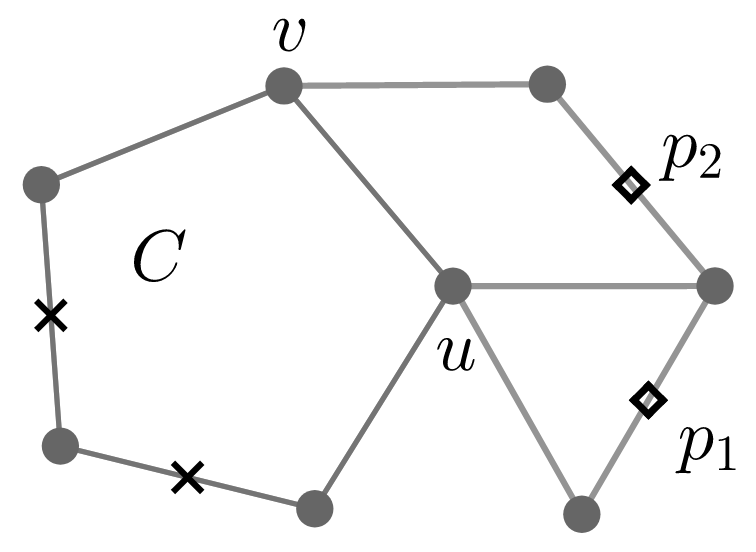
\includegraphics[scale=1.4]{Chaptercflg/media/cycle-cover-point.png}
	\caption{Two cycle coverage points with respect to a cycle $C$ of five nodes}
	\label{fig:cycle-cover}
\end{figure}
Discretization methods identify finite dominating sets (FDS), which are finite subsets of candidate locations guaranteed to contain an optimal solution. %Therefore, one can solve a reduced set-covering problem with continuous demands and finite candidate locations in FDS.
From the literature, we know at least three FDS for related variants of the CSCP, which rely on different assumptions on the network and the covering radius. Here, we review and compare these FDS. Since we aim to propose a general exact algorithm, we show that it may not be viable to extend discretization methods to solve the CSCP for general networks and real radii.

First, Church and Meadows \cite{Church79} studied the problem with demand at nodes, and identified the following points:
$$NIP:=\{p\in C(N):\: d(p,v)=\delta \:\textup{ for some }v\in V \}.$$
The authors proved that $FDS_1:=V\cup NIP$ is an FDS for the network set-covering problem when the set of demand points is $V$ and that of candidate locations is $C(N)$.

Secondly, Gurevich et al. \cite{Gurevich84} studied the continuous set-covering problem  when the covering radius and the edge’s lengths are natural numbers. They presented an FDS for the case of all edge lengths being one, which can be easily extended to the case of general edge lengths (see \cite{Hamacher20}),
$$FDS_2:=\big\{p\in C(N):\: d(p,v)=\frac{i}{2\cdot l_e} \:\textup{ for some }e\in E\textup{ and } v\in e;\: i=0,\ldots,2\cdot l_e\big\}.$$
Note that $FDS_2$ depends on the edge's length.

Lastly,  Fr\"ohlich et al. \cite{Hamacher20} proposed a different FDS for the same version of the continuous set-covering with natural numbers. The authors defined the following set of cycle coverage points:
\begin{equation*}
    \resizebox{0.91\hsize}{!}{$
CCP:=\left\{p\in C(N):\: d(p,C):=\min_{y\in C}\{d(p,y)\}=\left(\delta-\frac{l_C}{2}\right)\textup{ mod } \delta, \:p\notin C,\:\textup{ for a simple cycle }C\subseteq C(N)\right\}$,}
\end{equation*}
where $l_C$ is the total length of the cycle $C$. Suppose that a cycle $C$ is covered by a set of facilities. A cycle coverage point is the furthest point where a facility that contributes to cover $C$ can be moved without compromising the coverage of the cycle (if the rest of the facilities remain unchanged).

\Cref{fig:cycle-cover} illustrates this idea. In the depicted example, all edges have unit length and $\delta=2$. The figure depicts $p_1$ and $p_2$, which are CPP with respect to the cycle $C$ of five nodes. Note that $d(p_1,C)=d(p_2,C)=1.5(=(2-5/2)\textup{ mod } 2)$. \Cref{fig:cycle-cover} also depicts two locations in $C$ (marked with symbols 'x'), which correspond to two possible feasible locations for the remaining facility needed to cover $C$ (note that the one at the bottom only yields a covering of the cycle if $p_2$ is located, while the other one together with either $p_1$ or $p_2$ can completely cover $C$).

The authors of \cite{Hamacher20} gave the following recursive definition of an FDS for the problem with natural numbers:
$$S_1:=V\cup NIP \cup CCP;$$
$$S_{j+1}:=S_j\cup\{p\in C(N):\: d(p,y)=\delta \textup{ for some } y\in bd(\cA(S_j)) \};$$
$$FDS_3:=S_{|J|},$$
where $bd(\cA(S_j))$ is the boundary of the area covered by $S_j$, and  $J\subseteq E$ is the subset of edges to be covered. As the author explained themselves, $FDS_3\subseteq FDS_2$. However, the cardinality of $FDS_3$ may be exponential in the input size, as the number of cycles in a network is in general exponential.

\begin{figure}
	\centering
	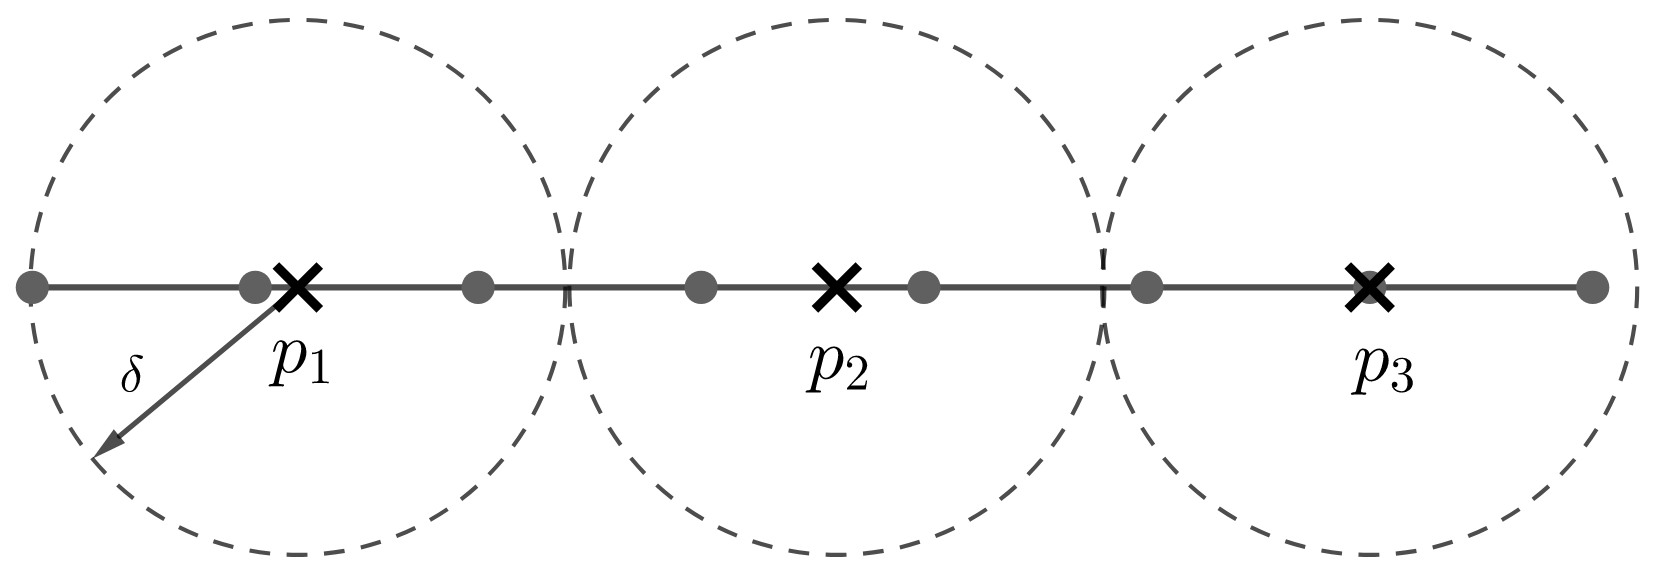
\includegraphics{Chaptercflg/media/discrete-covering2.png}
	\caption{An instance of CSCP such that not all facilities in $\mathcal{P}^*$ are at a distance $\delta$ from some node}
	\label{fig:exDiscrete}
\end{figure}
The example depicted in \Cref{fig:exDiscrete} illustrates that none of $FDS_1$ and $FDS_2$ are FDS for the CSCP. A similar observation was already presented in \cite{Kalsics} for a related problem. The figure shows eight nodes on a path, where all edges have equal lengths. If $l_e=1$ for all $e\in E$ and $\delta=1.2$, $\cP:=\{p_1,p_2,p_3\}$ is an optimal $\delta$-cover.

It can be easily observed that there is no optimal solution in which $p_2$ is placed either at a node or at a distance $\delta$ from some of the eight nodes, which shows that $FDS_1$ is not a valid FDS. On the other hand, it is also easy to check that there is not a feasible solution with the three facilities located either at nodes or middle-points of edges, which proves that $FDS_2$ is also not a valid FDS. As opposed to $FDS_2$, the assumption of the edge lengths and coverage radius being natural numbers is not fundamental in the definition of $FDS_3$. Conversely, $FDS_3$ is based on the idea of identifying those points at the ``boundaries'' of coverage areas, i.e., those delimiting the transition from covering/not covering a specific part of the network.


Consequently, $FDS_3$  could be extended to the general CSCP. However, such an extension potentially yields sets with many more candidates, due to the recursive construction of $FDS_3$ based on the distance function. Note that, if $\delta$ and the edge lengths are natural numbers, $FDS_3$ only contains points of the set
$$INT:=\{p\in C(N): d(p,v)\textup{ is integer or half-integer for some } v\in V\}.$$
Indeed, if $\delta\in \mathbb{N}$, $NIP\subseteq INT$ is clear; $CCP\subseteq INT$ holds since the operation $(\delta-{l_C}/{2})\textup{ mod } \delta$ only yields half integers; and $FDS_3\subseteq INT$ then easily follows by definition. However, if $\delta\in \mathbb{R}$, the locations of the points in $FDS_3$ are a priori undetermined, and its cardinality increases. Take the same example depicted by \Cref{fig:cycle-cover}. If $\delta=2.1$ (i.e. we increase $\delta$ just by 0.1), the CCP with respect to the cycle $C$ of the Figure increases from two to four points.






\subsection{Literature review}

Facility location and set covering problems have many variants and applications in operations research and management science. Related literature to this work is vast; here we review a selection of works related to CSCP. In \cite{sadigh2010mixed}, the model allows that an edge is covered jointly by two facilities. In \cite{Schobel2019}, the authors presented a unified vision of the common characteristics of facility location problems in a continuous space. In \cite{puerto2018extensive}, the authors summarized the research progress in facility location problems on networks. A recent survey \cite{wang2021emergency} provided a comprehensive overview of  emergency facility location problems in logistics, including mathematical models, applications, and the commonly used solution methods.  One of the most distinguishing features of variants of the maximal covering location problem is the solution space: continuous \cite{chapter-plastria, bansal2017planar}, discrete \cite{chapter-marin, cordeau2019benders}, or on networks \cite{bucarey2022benders,berman2016covering}. Especially in \cite{berman2016covering}, the authors  introduced the maximal covering location problem with edge demand. In \cite{baldomero2022upgrading}, the authors studied the upgrading version of the maximal covering location problem with edge length modifications on networks. A related problem that has been recently studied is the obnoxious facility location problem \cite{drezner2018weber}. It aims at locating undesirable facilities that have a negative impact on communities. The most common  objective is to maximize the shortest distance to the closest facility, and the problem has various variants featuring multiple facilities on the plane \cite{drezner2019planar,kalczynski2021obnoxious}, $p$-median objective \cite{kalczynski2022obnoxious}, or edge demand on networks \cite{berman2016covering}. We refer to \cite{church2022review} for a recent review on the obnoxious facility location problem. For more related works, we refer to \cite{akgun2015risk,paul2017multiobjective,fukunaga2016covering,berman2011big,hudec1994confined}. 

\subsection{Contribution}
As opposed to discretization methods, we directly tackle the CSCP for general networks and real radii.
Our main contribution is an exact integer programming approach for the CSCP, together with tailored algorithms and strategies to tackle it. Even if this problem has been known for decades, surprisingly, only a few partial results are known for some special cases and sub-classes of networks. To the best of our knowledge, only one MILP model \cite{Hamacher20} has been proposed so far which can address the general CSCP. Such a model can be applied to any network whose edges do not measure more than the covering radius. This condition does not restrict the applicability of the MILP in \cite{Hamacher20}, as any network can be transformed into an equivalent one that satisfies it.

Here, we present an enhanced MILP formulation that relies on the same assumption as that in \cite{Hamacher20}, but whose numbers of constraints and variables have smaller order of magnitude. In addition, preprocessing strategies to reduce the number of variables of the model are studied, and tailored algorithms are presented. Approaches to strengthen this formulation are also presented, including big-M constants tightening and valid inequalities. The valid inequalities are constraints that reduce the feasible space without removing model solutions.

The introduction of a second MILP, which is scalable concerning the edge's lengths completes the main contributions of this work. This second MILP is an adaptation of the first one we propose, with the difference that it does not require all edge lengths to be smaller than the covering radius. Finally, our computational experiments prove that the MILP model in \cite{Hamacher20}  is not scalable. On the other hand, the preprocessing technique drastically reduces the size of the first model proposed herein.

Finally, we show in the experiments that the second model we propose is superior to both  the model from \cite{Hamacher20} and our first model, in terms of the solution quality and solving time.

In the proposed setting, both the candidate facility locations and the demand points are continuous sets (in particular, they coincide with $C(N)$). The problem could be defined for a subset of demand edges, $J\subseteq E$, and/or a subset of candidate locations $H\subseteq E$. The theoretical results, model, and methods described in this work apply to such cases, after straightforward adaptation.


\subsection{Outline the chapter}
The rest of the chapter is organized as follows. \Cref{sec:prelim} presents useful notation and the theoretical development upon which our model is built. Then, our first MILP model is introduced in \Cref{sec:milp}, while strategies to strengthen this model are described in the next section. The network processing algorithms that complement our MILP are detailed in \Cref{sec:prepro}. A second MILP model, which we call reduced formulation and is a modification of the first MILP, is presented in \Cref{sec:reduced-milp}. Finally, \Cref{sec:compu} describes our computational experiments, and reports and analyzes the obtained results. \Cref{sec:conclu} closes the chapter with some conclusions.





\section{Covering characterization}\label{sec:prelim}
This section presents several notation, definitions, assumptions, observations, and results related to the CSCP. On the one hand, \Cref{thm.cover} gives a characterization of the $\delta$-covers of a network, which is based on the individual coverage of each edge of the network. Then, this result is refined to obtain a second necessary and sufficient covering condition in \Cref{cora.covercond}. It distinguishes between two alternative possibilities for covering each edge, namely complete or partial, and will be useful for our MILP formulation and methods. The rest of the section is oriented to characterize the so-called partial and complete covers. The idea of these sets is to delimit the areas of the network where a facility, if placed, would completely cover a given edge, and those where a facility would reach the edge (but maybe not completely cover it).




We first introduce some related notation, definitions and assumptions.
We assume that $V$ is totally ordered by the binary relation $\preceq$. Every edge $e \in E$ has a unique representation, $e = (v_a, v_b)$, where $v_a, v_b \in V$, and $v_a \preceq v_b$. From now on, we take $e=(v_a, v_b)$ indifferently as a continuum in $C(N)$ or as an edge ending at  $v_a, v_b$. We extend the edges' length function to  $l: C(N) \to \bR_+$ as a length measure on the continuum of points.   For two points $p, p' \in C(N)$, we denote by $\Pi(p,p') \subseteq 2^{C(N)}$ and $\Pi^*(p,p') \subseteq \Pi(p,p')$ the set of paths and shortest paths, respectively, connecting $p$ and $p'$. Any path $\pi\in \Pi(p,p')$ is indifferently treated as a continuum in $C(N)$, then $l_{\pi}:=l(\pi)$ is the length of $\pi$.  The distance between $p$ and  $p'$, $d(p, p')$, is the length of a shortest path connecting them:
$$d(p,p') := \min\{l_{\pi}: \:\pi\in \Pi(p,p')\}=l_{\pi^*} \textup{ for any } \pi^*\in \Pi^*(p,p').$$
In particular, if $p$ and $p'$ belong to the same edge, we denote by $l(p,p')$ the length of the unique path in that edge connecting them.
We work under the following assumption:
\begin{assumption} \label{assumption}
$\delta \ge l_e$ for all $e \in E$.
\end{assumption}
If Assumption \ref{assumption} did not hold, we could consider a set $I \subset  2^{C(N)}$, that would contain, for each $e = (v_a, v_b) \in E$, the following continuum sets of points (segments):
\begin{itemize}
	\item If $\delta \ge l_e$, $e \in I$;
	\item If $\delta < l_e$, let  $n:= \ceil{\frac{l_e}{\delta}}+1$. We define $v_1:= v_a$, $v_n:= v_b$ and $v_2,\hdots, v_{n-1}\in e$ such that $l(v_a,v_i) = (i -1) \frac{l_e}{n-1}$ for $i=2,\ldots, n-1$. Then, $(v_{i}, v_{i+1}) \in I$ for all $i=1,\ldots,n-1$.
\end{itemize}
We consider $N'=(V',E'=I)$, where $V'$ contains the endpoints of $I$. The new network $N'$ satisfies that $\delta \ge l_e$ for all $e\in E'$, and it is isomorphic to $N$ with respect to the length function. Indeed, since $N'$ is obtained by subdividing edges in $N$,  $C(N)=C(N')$ and a set of points $\delta$-covers $N$  if and only it $\delta$-covers $N'$. Therefore, Assumption \ref{assumption} always holds after the network $N$ is transformed into $N'$ (via a preprocessing step). Such transformation yields a network with more nodes and edges, which has a direct impact on the size of optimization models. In \Cref{sec:reduced-milp}, we present a model that avoids this effect.  

\subsection{Observations}
In the following, we give several observations of optimal $\delta$-covers, which guide our quantitative analysis of covering conditions and the resulting MILP model of \Cref{sec:milp}.

\begin{observation}
For an edge $e=(v_a, v_b) \in E$ and a point $p \in C(N)$, one of the following cases holds:
\begin{enumerate}
	\item   $p$ cannot $\delta$-cover any point in $e$;
	\item $p$ can $\delta$-cover the whole $e$;
	\item $p$ can $\delta$-cover a continuous portion of $e$ containing either $v_a$ or $v_b$;
	\item $p$ can $\delta$-cover two continuous portions of $e$, which do not intersect, each contains either $v_a$ or $v_b$.
\end{enumerate}
\end{observation}

\begin{observation}{(a similar statement was proven in \cite{Hamacher20})}
There exists an optimal $\delta$-cover that satisfies:
\begin{enumerate}
	\item[i)] Each edge $e \in E$ has at most two facilities (due to Assumption \ref{assumption});
	\item[ii)] If there are two facilities in the edge $e$, we can assume without loss of generality that they are located at end nodes $v_a$, $v_b$ (this follows from i) and  Assumption \ref{assumption}).
   % \item[iii)] If there is a facility placed in $\inter(e)$, $e \in E$, then $e$ contains a single facility.
\end{enumerate}
As a consequence, the set of candidate facilities of a $\delta$-cover is in one-to-one correspondence to the edges and nodes of the network.
\end{observation}

With the above observations, we can already give a high-level description of the covering characterization behind our model. %Naively, one can search the edges and nodes that host a facility. Given such host edges and nodes, the cover is already partially fixed:
Namely, if we fix a set of facilities on some network edges, there would be some edges completely covered regardless of the exact facility locations within their edges. Some other edges would be partially covered from the left-end node and/or from the right-end node, and how much
depends on the actual facility locations. So we have variables that
specify the exact facility locations on each edge. Finally, we stipulate that the cover from the left and the cover from the right better exceed the edge length. %However the cover of an edge depending on the exact facility location on this edge
One difficulty is that the corresponding covering function
is not linear %function (and bad for an LP).
However, we show that such a function is a piece-wise linear function, which can be modeled by a MILP. The aim of the remainder of this section is to give a mathematical  specification of the above characterization.



\subsection{Covering conditions}
We give a sufficient and necessary condition that the network is $\delta$-covered by installed facilities.
 
 \begin{proposition}
 \label{thm.cover}
Let $\cP=\{p_i\}_{p_i\in C(N)}$ be a finite set  of points in $C(N)$. An edge $e=(v_a, v_b) \in E$ is $\delta$-covered by $\cP$ if and only if either there exists $p \in \cP\cap e$ or
 \begin{equation}
	\label{eq.covercond}
    	\max\{\delta -  \min_{p \in \cP} d(v_a,p),0\} +  \max \{\delta - \min_{p \in \cP} d(v_b,p), 0 \} \ge l_e.
	\end{equation}
Moreover, the set $\cP$ is a $\delta$-cover of $N$ if and only if for each $e\in E$, either there exists $p \in \cP\cap e$ or \eqref{eq.covercond} is satisfied.
\end{proposition}
\begin{proof}  
If there exists $p\in \cP\cap e$, then $e$ is $\delta$-covered by $p$ due to Assumption \ref{assumption}.
Otherwise, for each $i\in\{a,b\}$, let us consider $p^*_i \in \cP$ such that $d(v_i,p^*_i)=\min_{p \in \cP} d(v_i,p)$ and let  $\pi^*_i\in \Pi^*(v_i,p_i^*)$ be a shortest path between $v_i$ and $p_i^*$, i.e. $l_{\pi^*_i}= d(v_i,p^*_i)$. Condition \eqref{eq.covercond} can be rewritten as follows:
$$ \max\{\delta - l_{\pi^*_a},0\} +  \max \{\delta - l_{\pi^*_b}, 0 \} \ge l_e.$$
Note that $\max\{\delta - l_{\pi^*_i},0\} $ represents the maximum length that can be $\delta$-covered by $\cP$ (specifically, from $p^*_i$) after passing through $v_i$. Since the path(s) that $\delta$-cover $e$ must contain $v_a$ and/or $v_b$, the edge is covered if and only if these ``maximum lengths'' for $v_a$ and $v_b$ add up to more than $l_e$.


\end{proof}
\begin{figure}
	\begin{subfigure}{0.33\textwidth}
	\centering
   	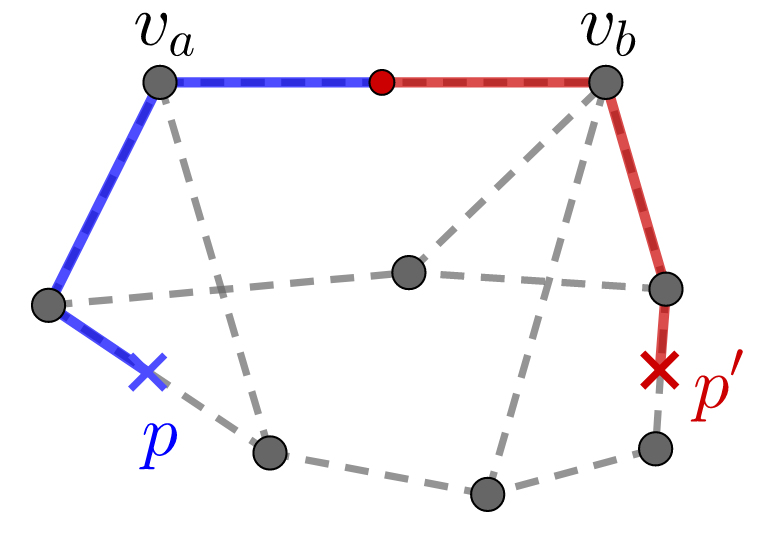
\includegraphics[scale=1]{Chaptercflg/media/example-Theo.png}
   	\caption{By two points}
   	\label{fig:teoex-a}
	\end{subfigure}
	\begin{subfigure}{0.33\textwidth}
	\centering
   	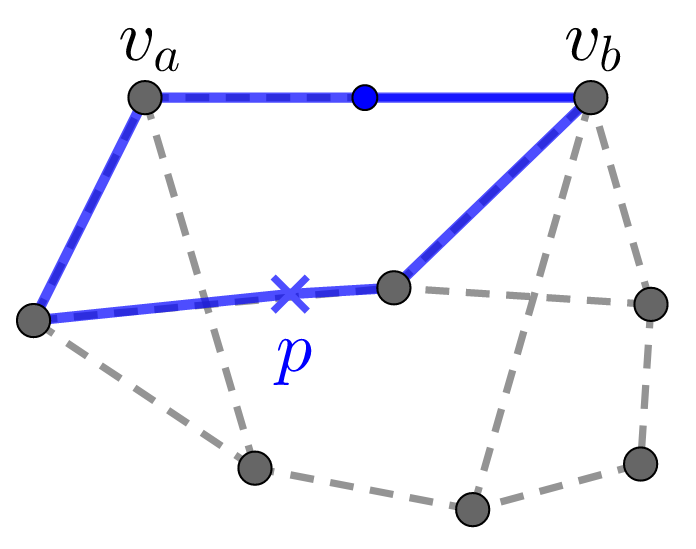
\includegraphics[scale=1]{Chaptercflg/media/example-Theo3.png}
   	\caption{By one point, through both ends}
   	\label{fig:teoex-b}
	\end{subfigure}
 	\begin{subfigure}{0.33\textwidth}
	\centering
   	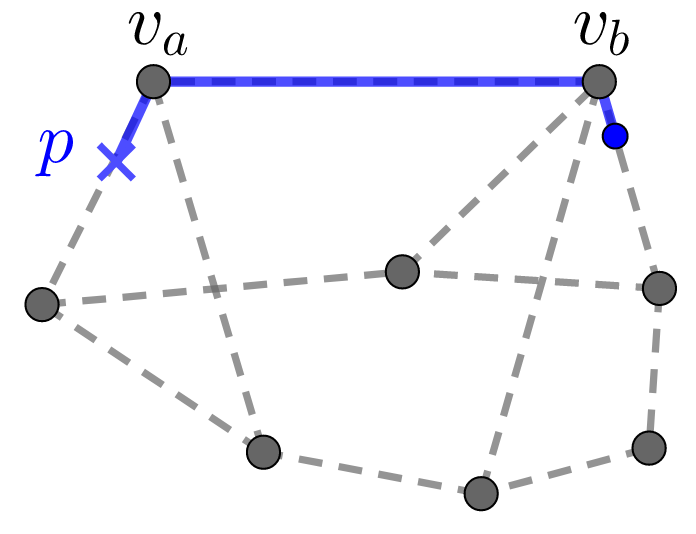
\includegraphics[scale=1]{Chaptercflg/media/example-Theo2.png}
   	\caption{By one point, through one end}
   	\label{fig:teoex-c}
	\end{subfigure}
	\caption{Covering of an edge $e=(v_a,v_b)\in E$}
	\label{fig:teoex}
\end{figure}
\Cref{fig:teoex} illustrates \Cref{thm.cover}. It shows three ways of covering the same edge $e=(v_a,v_b)\in E$ for a given network. The edges of the network are depicted with dashed lines, while the different paths through which $e$ is covered are delimited with continuous bold traces. Facility locations are marked with the symbol `x'. \Cref{fig:teoex-a} depicts two facilities located at $p,p'$ that cover two portions of the edge, which contain $v_a$ and $v_b$ respectively. In this case, the $\min$ functions inside \eqref{eq.covercond} are attained respectively at $p$ and $p'$. In the middle,  \Cref{fig:teoex-b} shows a single location $p$ that covers $e$ through two different paths, which traverse $v_a$ and $v_b$ respectively. These paths form a cycle that contains $p$ and $e$. In this case,  the two $\min$ operations inside \eqref{eq.covercond} are attained at the same point, $p$. Finally, \Cref{fig:teoex-c} illustrates the case in which a single facility located at $p$ covers $e$ through one of its end nodes, $v_a$. Here, one of the $\max$ operators in \eqref{eq.covercond} is equal to zero ($p$ is further from $v_b$ than $\delta$).

\subsection{Covering delimitation and simplification}
\label{sec.subc}

For an optimization or search problem, \textit{delimitation} refers to the reduction of the candidate space. FDS is studied in related works as a way for reduction of CSCP (under some assumption), and hence it is a kind of delimitation. Instead of FDS, we consider a different delimitation that can be used for the general CSCP, and which allows us to obtain a reduced MILP formulation.

The characterization in \Cref{thm.cover} is based on the individual covering of every edge in the network. When considering possible locations to cover a fixed edge, we can restrict ourselves to its surroundings within the radius $\delta$. Delimiting those parts of the network that could ``contribute'' to covering a particular edge or node reduces the search space. We  then introduce three kinds of delimitation: \textit{potential covers}, \textit{complete covers} and \textit{partial covers}.   We will represent the covering condition under such delimitation. In effect, the covering condition has a simplified form compared to its general form in \Cref{thm.cover}, and an adequate preprocessing procedure can reduce and strengthen our MILP model.

We find that, for every node, there may exist potential covers, i.e., a set of edges and nodes where, if a facility is located, it can \textit{possibly} $\delta$-cover this node.  The potential covers in the following definition delimit the edges and nodes of $C(N)$ that can contribute to covering a particular node of the network.
\begin{definition}\label{defa.linksetsv}
For each $v \in V$, the potential covers of $v$ are the candidate facility locations to cover $v$:
\begin{align}
 \cE(v)&:= \{e'=(v'_a,v'_b) \in E:\:   d(v,v'_{i}) \le \delta \textup{ for some } i\in \{a,b\} \} \nonumber\\
 \cV(v)&:= \{v' \in V: \:  d(v,v') \le \delta\} \nonumber\\
 \cF(v)&:= \cE(v) \cup \cV(v). \nonumber
\end{align}
\end{definition}
Clearly, $v$ is not reachable within the radius $\delta$ for any facility installed outside $\cF(v)$. Regarding the covering of edges, an edge incident to $v$ could be covered by some of the facilities in $\cF(v)$.

We find that, for every edge $e$, there may exist complete covers, i.e., a set of edges and nodes where, if a facility is located, it can \textit{always} $\delta$-cover the edge $e$, regardless of the exact facility location. Once there is a facility within a complete cover, the whole edge $e$ is guaranteed to be covered by this facility. The following definition serves to delimit the network to such complete covers.

\begin{definition}
\label{def.linksetse}
For each $e=(v_{a}, v_{b}) \in E$, the  complete covers of $e$ are the candidate facility locations that can completely cover $e$:
\begin{align}
\cE_{\mathrm{c}}(e)& :=\{e' \in E:   \forall p' \in e', \forall  p \in e,\:   d(p,p') \le \delta\}\nonumber\\
   \cV_{\mathrm{c}}(e)&:= \{v' \in V:   \forall  p \in e,\: d(p,v') \le \delta \}\nonumber\\
  \cF_{\mathrm{c}}(e) &:= \cE_{\mathrm{c}}(e) \cup \cV_{\mathrm{c}}(e).
\end{align}
\end{definition}
If a facility is placed at $\cF_{\mathrm{c}}(e)$ (either at a node in $\cV_{\mathrm{c}}(e)$ or at a point on an edge belonging to $\cE_{\mathrm{c}}(e)$), we can immediately conclude that $e$ is $\delta$-covered.
Note that any facility placed at $e'$ can completely cover $e$ if and only if any facility placed at $e$ can completely cover $e'$. That is,  $\cE_{\mathrm{c}}$ is symmetric over $E$. On the other hand, it is obvious that $e\in \cE_{\mathrm{c}}(e)$,  and $v_{a} ,v_{b}\in \cV_{\mathrm{c}}(e)$, for all $e=(v_a,v_b)\in E$.


Given a node $v$, we can characterize the complete covers of the incident edges to the node $v$. This helps us refine the potential covers of this node.  The following definition  identifies those candidate facility locations in the potential covers of the node $v$ that cannot completely cover any incident edges to $v$.
\begin{definition} \label{defa.linksetsvincident}
We define the following sets for each $v\in V$:
\begin{align}
\cE_{\mathrm{p}}(v)&:=\{e'\in \cE(v):\: \exists e\in E(v),\: e'\notin\cE_{\mathrm{c}}(e)\} \nonumber\\  \cV_{\mathrm{p}}(v)&:=\{v'\in \cV(v):\: \exists e\in E(v),\: v'\notin\cV_{\mathrm{c}}(e)\}   \nonumber\\
\cF_{\mathrm{p}}(v)&:=\cV_{\mathrm{p}}(v)\cup\cE_{\mathrm{p}}(v).
\end{align}
We call these sets the \emph{partial covers} of $E(v)$, where $E(v):=\{e\in E:\: v\in e\}$ is the set of incident edges to $v$.
\end{definition}
The set $\cF_{\mathrm{p}}(v)$ contains those candidate locations that can contribute to partially covering some of the edges in $E(v)$. Note that, if a facility is placed at $\cF(v)\setminus \cF_{\mathrm{p}}(v)$, then this facility completely covers  $E(v)$.

Definitions  \ref{defa.linksetsv}, \ref{def.linksetse}, and \ref{defa.linksetsvincident}  provide us with a refined covering condition. Indeed, the following proposition is a consequence of \Cref{thm.cover} and the aforementioned definitions, and will be used to characterize coverings in the MILP formulation presented in \Cref{sec:milp}.

\begin{proposition}
\label{cora.covercond}
A finite set $\cP$ of points in $C(N)$  is a $\delta$-cover of $N$ if and only if,
for each $e=(v_a,v_b) \in E$, either $\cP \cap \cF_{\mathrm{c}}(e) \ne \varnothing$ or
\begin{equation}
\label{eqa.coverdistfull}
	\sum_{i \in \{a,b\}} \max \big\{0,\delta -  \min_{p \in   \cP \cap \cF_{\mathrm{p}}(v_i)} d( v_{i}, p)\big \} \ge l_e.
\end{equation}
Moreover,
\begin{equation}\nonumber
\begin{split}
\min_{p \in \cP \cap \cF_{\mathrm{p}}(v_i)}d(v_{i}, p)
   = &\min \left\{\min_{v' \in \cP \cap \cV_{\mathrm{p}}(v_i)} d(v_{i}, v'), \min_{p \in  \cP \cap (\cE_{\mathrm{p}}(v_i)\setminus  V)}  d(v_{i}, p) \right\}, \textup{ for } i=a,b.
\end{split}
\end{equation}
\end{proposition}
\begin{proof}
For $i \in \{a,b\}$, the equality $\cF(v_i)=\cF_{\mathrm{p}}(v_i)\cup\cF_{\mathrm{c}}(e)$ holds by definition, which gives the new necessary and sufficient covering condition.

For the second statement of the proposition, we have $\cF_{\mathrm{p}}(v_i)=\cV_{\mathrm{p}}(v_i)\cup \cE_{\mathrm{p}}(v_i)$ from Definition \ref{defa.linksetsvincident}. Then, it suffices to see that we can take $p \in  \cP \cap (\cE_{\mathrm{p}}(v_i)\setminus  V)$ in the second inner $\min$ operator of the right-hand side instead of $p \in  \cP \cap \cE_{\mathrm{p}}(v_i)$. Let $e'=(v'_a,v'_b)\in  \cE_{\mathrm{p}}(v_i)$. We prove that the end nodes of $e'$ can be excluded from the second inner $\min$ operator.  Let $i' \in \{a,b\}$, we denote $\bar{i'}=b$ if $i'=a$ and $\bar{i'}=a$ if $i'=b$.  First, by definition, $d(v_i,v'_{i'})\leq \delta$ for some $i'\in\{a,b\}$. Therefore, $v'_{i'}\in \cV_{\mathrm{p}}(v_i)$, and we can exclude it from the second inner $\min$ operator (this node is already considered by the first inner $\min$ operator). We consider now the other end node of $e'$. If $d(v_i,v'_{\bar i'})\leq \delta$ then, similarly, $v'_{\bar{i}'}$ can be excluded from the second inner $\min$. Otherwise, we know that the outer $\min$ is not attained at $v'_{\bar i'}$, as  $d(v_i,v'_{i'})\leq \delta < d(v_i,v'_{\bar i'})$, thus $v'_{\bar i'}$ can be disregarded.
\end{proof}

\begin{remark}
    The left hand side function in \eqref{eqa.coverdistfull} is a PWL function w.r.t.  the distance $d$. Moreover, we cannot reformulate it into a system of linear constraints,  because the left hand side function involves the max functions, which is convex w.r.t. its argument. In this chapter, we consider a big-M method to reformulate the PWL function as a MILP representable function.
\end{remark}

\begin{remark}
The covering conditions described both in Propositions \ref{thm.cover} and \ref{cora.covercond} would be also applicable if only a subset of $E$, $J\subseteq E$, is to be covered. Indeed, these covering conditions are based on the individual coverage of the edges, so it would be sufficient to apply them just to the edges in $J$. As a consequence, our methods, including the MILP formulation and algorithms presented in the next sections, apply to this more general version of the CSCP.
\end{remark}



In order to exploit the newly defined potential, complete, and partial covers in our formulation, from a practical viewpoint, we need to have some characterizations that can operate in a computer. Definition \ref{defa.linksetsv}, which introduces potential covers, satisfies this requirement. Indeed, it just depends on distances between pairs of nodes, which we can easily calculate. Conversely, Definition \ref{def.linksetse} presents complete covers with a condition that must be satisfied by ``the infinitely many points of an edge'', which is not directly computable. Finally, the elements in the partial covers defined by Definition \ref{defa.linksetsvincident} can be easily calculated once both potential and complete covers are known.

\subsection{Characterization of complete covers}

In the following, we focus on characterizing the complete covers, which will be useful for our MILP formulation and tailored algorithms, (see forthcoming Sections \ref{sec:milp} and \ref{sec:prepro}). To begin with, we note that \Cref{thm.cover} already gives us a characterization of the nodes in $\cV_{\mathrm{c}}(e)$. Indeed, it is easy to observe that, for a given $e\in E$, $v\in \cV_{\mathrm{c}}(e)$ if and only if $\cP:=\{v\}$ $\delta$-covers $e$. We then focus on the sets $\cE_{\mathrm{c}}(e)$. On the one hand, it is clear that, for every edge $e=(v_a,v_b)\in E$,
$$\cE_{\mathrm{c}}(e)\subseteq \cE(v_a)\cap \cE(v_b).$$
Moreover, if we define $\cE_{\mathrm{c}}(v)\subseteq \cE(v)$ as follows, we have a tighter set containing $\cE_{\mathrm{c}}(e)$.
\begin{definition}\label{def.cEc}
The edges that can completely cover a node $v \in V$ are:
$$\cE_{\mathrm{c}}(v) :=\{e' \in E:   \forall p' \in e',\:   d(v,p') \le \delta\}.$$
\end{definition}

It is clear that the following observation holds.
\begin{observation}\label{obser}
For any $e=(v_a,v_b)\in E$, $\cE_{\mathrm{c}}(e)\subseteq \cE_{\mathrm{c}}(v_a)\cap \cE_{\mathrm{c}}(v_b)$.
\end{observation}
With this observation, we can limit the search of $\cE_{\mathrm{c}}(e)$ in the set $\cE_{\mathrm{c}}(v_a)\cap \cE_{\mathrm{c}}(v_b)$, as we will show in \Cref{sec:prepro}, the latter set is easy to compute.



We recall that Definition \ref{def.cEc} is somewhat the inverse of Definition \ref{def.linksetse}. That is,  $e'\in \cE_{\mathrm{c}}(v)$ if and only if $v \in \cV_{\mathrm{c}}(e')$. We present a set of intermediate statements in Definition \ref{def.function}, Lemma \ref{lem.covercE}, and Lemma  \ref{lem.pieces}, which allow us to describe the edges in the complete cover set $\cE_{\mathrm{c}}(e)$ as the main result in \Cref{prop.chara.cEe}.

\begin{definition}\label{def.function}
Let $v\in V$ be a node and $e'=(v'_a,v'_b)\in E $ be an edge. For all $q \in [0, l_{e'}]$, we define the following functions:
\begin{align}
	d_v(q) &:= \min \{d(v,v'_a)+q, d(v,v'_b)+l_{e'}-q\} \nonumber\\
	r_v(q) &:= %\max\{\delta -  \min \{d(v,v'_a)+q, d(v,v'_b)+l_{e'}-q\},0\} =
	\max\{\delta -  d_v(q),0\}, \nonumber
\end{align}
and constant:
$$Q_{ve'}:=(d(v,v'_b)+l_{e'} - d(v,v'_a))/2,$$  which satisfies the following equation:
$$d(v,v'_a)+Q_{ve'}=  d(v,v'_b)+l_{e'}-Q_{ve'}.$$
\end{definition}
The function $d_v(q)$ represents the distance between $v$ and a point $p'\in e'$ such that $q=l(v'_a,p')$, where $l(v'_a,p')$ measures the length of the continuum $(v'_a,p')\subseteq e'$.
The inner terms in the minimization that defines $ d_v(q)$ coincide for $q=Q_{ve'}$. Informally, $Q_{ve'}$ is the ``bottleneck" coordinate on $e'$ (see original definition in \cite{obnoxious}), for which the distance to $v$ is the same if we go through $v'_a$ or $v'_b$. Indeed, since $|d(v,v'_b) - d(v,v'_a)| \le l_{e'}$, it follows that $0 \le Q_{ve'} \le l_{e'}$.
Note that $d_v(q)$,  $r_v(q)$, and $Q_{ve'}$ depend also on the edge $e'$.

\begin{lemma} \label{lem.covercE}
Let $e=(v_a,v_b)$. An edge $e'$ is in $\cE_{\mathrm{c}}(e)$ if and only if $ r_{v_a}(q)+r_{v_b}(q)\geq l_e$ for all $q\in [0,l_{e'}]$.
\end{lemma}
\begin{proof}
$e' \in \cE_{\mathrm{c}}(e)$ if and only $e$ is $\delta$-covered by any point $p' \in e'$.
Take $\cP = \{p'\}$ in \Cref{thm.cover}, $e$ is $\delta$-covered by $\cP$, if and only if
 \begin{equation*}
 \max\{\delta -  d(v_a,p'),0\} +  \max\{\delta -  d(v_b,p'),0\} \geq l_e
\end{equation*}
holds for all $p'\in e'$. Let $q=l(v'_a,p'),\: q \in [0, l_{e'}]$, be the measure of the sub-edge $(v'_a,p')\subseteq e'$. Then, the observation that $d_{v_i}(q)=d(v_i,p')$ for $i=\{a,b\}$ completes the proof.
\end{proof}

We present the following lemma without proof. The lemma is a direct consequence of Definition \ref{def.function}.
\begin{lemma}\label{lem.pieces}
Let $v\in V$ and $e'=(v'_a,v'_b)\in E$. Then, $0 \le Q_{ve'} \le l_{e'}$, the function $d_v(q)$ is increasing when $q\in [0, Q_{ve'}]$, and it decreases for $q\in[Q_{ve'}, l_{e'}]$. Moreover, $d_v(q)$ admits the following piece-wise linear representation:
\begin{equation*}
	d_v(q) = \begin{cases}
	d(v,v'_a)+q & \textup{ if }q \le Q_{ve'}, \\
	d(v,v'_b)+l_{e'}-q & \textup{ if }q \ge Q_{ve'}. \\   
	\end{cases}
\end{equation*}
\end{lemma}

Note that with  \Cref{obser}, to find $\cE_{\mathrm{c}}(e)$, we can check \Cref{lem.covercE} for $e' \in \cE_{\mathrm{c}}(v_a) \cap \cE_{\mathrm{c}}(v_b)$: if $ r_{v_a}(q)+r_{v_b}(q)\geq l_e$, then $e'$ is in  $\cE_{\mathrm{c}}(e)$. Then, we consider $v \in V$, and we want to characterize $r_v$ for all points on edges $e'\in E$ such that $e' \in \cE_{\mathrm{c}}(v)$. We present the following result without proof.


\begin{lemma}
Given $v \in V$, and $e'=(v'_a,v'_b) \in \cE_{\mathrm{c}}(v)$. If $e'\in \cE_{\mathrm{c}}(v)$, then $r_v(q)$ admits the following piece-wise linear representation:
\begin{equation*}
	r_v(q) = \begin{cases}
	\delta - (d(v,v'_a) + q) & \textup{ if }q \le Q_{ve'}, \\
	\delta- (d(v,v'_b)+l_{e'}-q) & \textup{ if }q \ge \ Q_{ve'}. \\   
	\end{cases}
\end{equation*}
\end{lemma}

Finally, we have a tractable version of \Cref{lem.covercE}.

\begin{proposition}\label{prop.chara.cEe}
Let $e=(v_a,v_b)$. An edge $e'\in \cE_{\mathrm{c}}(v_a)\cap \cE_{\mathrm{c}}(v_b)$ is in $\cE_{\mathrm{c}}(e)$ if and only if
$$r(q)\geq l_e\quad \textup{for all}\quad q=Q_{v_ae'}, Q_{v_be'},$$
where $r(q):=r_{v_a}(q)+r_{v_b}(q)$.
\end{proposition}
\begin{proof}
From Lemma \ref{lem.covercE}, $e' \in \cE_{\mathrm{c}}(e)$ if and only if $\min_{q \in [0, l_{e'}]} r(q) \ge l_e$. Due to Lemma \ref{lem.pieces}, the minimum argument must be some of the breakpoints in the piece-wise linear description of $r_v(q)$. Then, it suffices to check
\begin{equation*}
	\min \{r(q):\: q \in \{0, Q_{v_ae'}, Q_{v_be'}, l_{e'}\}\} \ge l_e.
\end{equation*}

Since $e'\in \cE_{\mathrm{c}}(v_a)\cap \cE_{\mathrm{c}}(v_b)$, $r_{v_i}(0)\geq l_e$ and  $r_{v_i}(l_{e'})\geq l_e$  always holds for all $i\in\{a,b\}$.
 It suffices thus to check  the following condition
\begin{equation*}
	\min \{r(q):\: q \in \{ Q_{v_ae'}, Q_{v_be'} \}\}  \ge l_e.
\end{equation*}
Then, the result follows.
\end{proof}



\section{MILP formulation}\label{sec:milp}


We present the variables of the MILP formulation first. For each $v \in V$, there is one candidate facility (fixed location); and for each $e \in E$, there is another one (location within the interior of $e$, $e\setminus\{v_a,v_b\}$). Then, the finite set $\cF \coloneqq E \cup V$ will be used to index the candidate facilities.
In our MILP formulation, there are two decisions associated with each  $f\in \cF$. One is to decide if a facility is installed at $f$. The second is only necessary for those facilities installed at the interior of edges, and consists in determining their locations within the corresponding edges.

To represent the first of the above decisions, we define the following binary variables, which we call the \emph{placement variables}:
$$y_f=1 \textup{ if a facility  is installed at } f,\quad  \textup{ for all }f \in \cF.$$
We identify the set of installed facilities with $\cF_1 = \{f \in \cF: y_f = 1\}$. To represent the second of the above decisions, we define the following continuous variables, which we name the \emph{coordinate variables}:
$$q_e=
\begin{cases}
l(v_a,p) &\textup{ if } y_e=1 \textup{ and a facility is installed at } p\in e\\
0 &\textup{ otherwise}
\end{cases}
\qquad \textup{ for all }e=(v_a,v_b)\in E.$$



We use $v'$ and $e'$ to denote nodes and edges where facilities are installed,   and use $v$ and $e$ to denote  nodes and edges to be covered, respectively. We refer to $v_a, v_b$ as the end nodes of $e=(v_a,v_b)\in E$; given $e'=(v'_a,v'_b) \in E$, we refer to $v'_a, v'_b$ as its end nodes.


We use the necessary and sufficient condition of $\delta$-covering in \Cref{cora.covercond}, and the second result in this proposition regarding the distance function. Other than the placement and coordinate variables, some additional variables are used, which we present next.


\begin{itemize}
    \item  $\forall e \in E, w_e\in\{0,1\}$, if $\cF_{\mathrm{c}}(e)\cap \cF_1\neq \varnothing$, then $w_e = 1$;
\item $\forall  v \in V, r_{v}\in[0, +\infty)$; 
%\mer{$r_{v}\in[0, +\infty)$} & \mer{, $r_{v}$} $\leq \max\{0,\delta-  \displaystyle \min_{f\in \cF_{\mathrm{p}}(v) \cap \cF_1} \{\mer{d(v,p_f), \textup{ where } p_f \textup{ is the point on } f \textup{ where a facility is installed}}\}\}$ %the 'residual' cover at $v$
\item $\forall v \in V, x_{v}\in\{0,1\}, =1$, if $\forall e\in E(v)$, $ \cF_{\mathrm{c}}(e) \cap \cF_1 \ne \varnothing,$ then $x_v = 1$;
%$z_{vv'}\in\{0,1\}$ & $=1$ if $v'=  \displaystyle \argmin_{f \in \cF_{\mathrm{p}}(v) \cap \cF_1} \{d(v,p):\: \textup{a facility is installed at }p\in f\}$ & $ v \in V$, $v' \in \cV_{\mathrm{p}}(v)$;\\
%$z_{ve'{i'}}\in\{0,1\}$ & $=1$ if $e' =  \displaystyle \argmin_{f \in \cF_{\mathrm{p}}(v)\cap \cF_1 }\{d(v,p):\: \textup{a facility is installed at }p\in f\}$,\\
%& and $(e',i') = \displaystyle \argmin_{(e,i) \in \cEI_{\mathrm{p}}(v)} \tau_{vei}(q_{e})$  & $ v \in V$, $(e',i') \in \cEI_{\mathrm{p}}(v)$;
\item $\forall  v \in V$, $v' \in \cV_{\mathrm{p}}(v), z_{vv'}\in\{0,1\}$, if $ \forall e=(u,v)\in E(v)\mst w_e=0$, $\max\{0,\delta-d(v,v')\}+r_u\geq l_e$, then $z_{vv'} = 1$;
\item  $\forall v \in V$, $(e',i') \in \cEI_{\mathrm{p}}(v)$, if $\forall e=(u,v)\in E(v)\mst w_e=0$, $\max\{0,\delta- \tau_{ve'i'}(q_{e'})\}+r_u\geq l_e$, then $ z_{ve'{i'}}\in\{0,1\}=1$.
\end{itemize}

where $$ \tau_{ve'i'}(q) := d(v,v_{i'})+ \mathbf{1}_{i'=a}q +\mathbf{1}_{i'=b}(l_{e'} - q),$$ and $$\cEI_{\mathrm{p}}(v) := \{(e'=(v'_a,v'_b),i') \in \cE_{\mathrm{p}}(v) \times \{a,b\}:\: d(v,v'_{i'})\leq \delta\}.$$ We sometimes refer to $r_v$ as the ``residual cover'' at node $v$, since it represents the maximum remaining length that can be covered after reaching $v$ from ``a sufficiently close'' facility. Remembering \Cref{def.function}, these variables must satisfy:
$$r_v\leq r_v(q_e), \: \textup{ for all } e \in \cF_1 \cap (E \smallsetminus E(v)).$$
In an optimal solution, it can be $r_v=r_v(q_e)$ for an edge $e\in E$ as stated above. In this case, $r_v$ is the maximum remaining length that can be covered after reaching $v$ from the closest facility. However, we do not impose this equality in our formulation, since it is enough for guaranteeing the coverage of $e=(v_a,v_b)\in E$ that the sum of the residuals $r_{v_a}+r_{v_b}$ exceeds $l_e$ (see \Cref{cora.covercond}). That is, if $l_e$ is already exceeded by $r_{v_a}+r_{v_b}$  for some $r_{v_i} < r_{v_i}(q_e)$, then the coverage condition of \Cref{cora.covercond} will hold.

We denote by $M_{*}$ the sufficiently large big-M constant associated with index $*$, the value of which will be determined later. Our formulation of the CSCP reads as follows:
\begin{subequations}
	\label{milpa}
	\begin{align}
   	\min & \sum_{f \in \cF} y_f \label{milpa.obj} \\
	\mst   & w_{e} \ge y_{f}   &  e \in E, f \in \cF_{\mathrm{c}}(e) \label{milpa.completecover1}\\
      	& w_{e} \le  \sum_{f \in \cF_{\mathrm{c}}(e)}y_{f} 	&  e \in E \label{milpa.completecover2}\\
      	& x_{v}\geq 1-\sum_{e\in E(v)} (1-w_e) &  v\in V \label{milpa.enforcex1}\\
      	& x_{v}\leq w_e &  v\in V, e\in E(v) \label{milpa.enforcex2}\\
	&  y_{v'_{i'}} + y_{e'} \le 1 &   e' \in E, i' \in \{a,b\} \label{milpa.optimale}\\
	& q_{e'}\leq l_{e'}y_{e'} & e'\in E  \label{milpa.coord} \\
	&  l_e (1 - w_e) \le  r_{v_a} + r_{v_b}	& e \in E \label{milpa.covere}\\
  &  x_{v} +\sum_{v' \in \cV_{\mathrm{p}}(v)}  z_{vv'}+ \sum_{(e', i') \in \cEI_{\mathrm{p}}(v)} z_{ve'i'} = 1  &   v\in V \label{milpa.lcoversos} \\
  &   z_{vv'} \le y_{v'}  &  v \in V,  v' \in \cV_{\mathrm{p}}(v) \label{milpa.indicatorv}\\  
	&   z_{ve'i'} \le y_{e'}  &  v \in V,  (e',i') \in \cEI_{\mathrm{p}}(v) \label{milpa.indicatorei}\\  
 &   r_{v} \le M_v (1-x_{v}) &  v\in V \label{milpa.wbdl}\\
 &   r_{v} \le M_{vv'}(1 - z_{vv'})  +  \delta - d(v,v') & v \in V ,  v' \in \cV_{\mathrm{p}}(v) \label{milpa.coverdist-node} \\
 &   r_{v} \le M_{ve'i'}(1 - z_{ve'{i'}})  +  \delta - \tau_{ve'i'}(q_{e'}) & v \in V ,  (e',i') \in \cEI_{\mathrm{p}}(v) \label{milpa.coverdist-edge} \\
   &  y_f, w_e  \in \{0,1\} &   f \in \cF,  e \in E \label{milpa.varyw}\\
   & x_{v}, z_{vv'}, z_{ve'{i'}} \in \{0,1\}  & v \in V, v' \in \cV_{\mathrm{p}}(v),(e',i') \in \cEI_{\mathrm{p}}(v)\label{milpa.varindicator}\\
  	& q_{e'}, r_{v} \geq 0 &  e'  \in E, v \in V. \label{milpa.varcontinuous}
	\end{align}
	\end{subequations}
Constraints \eqref{milpa.completecover1} and \eqref{milpa.completecover2} model the logic or constraint $w_e = \lor_{f \in \cF_{\mathrm{c}}(e)} y_f$.  Constraints \eqref{milpa.enforcex1} and \eqref{milpa.enforcex2} enforce the logic constraint  $x_v = \land_{e \in E(v)} w_e$, that is, $x_v$ is the product of the $w_e$ variables such that $e\in E(v)$.  
Constraints \eqref{milpa.optimale} prevent two facilities in a solution from being installed respectively at the interior of an edge and one of their end nodes.
Constraints \eqref{milpa.coord} bound the coordinate variables with the corresponding edge length, and set them to zero if no facility is located at its interior.
The covering condition in \Cref{cora.covercond} is enforced by \eqref{milpa.covere}. If $w_e=1$, then the condition is satisfied ($e$ is covered by $\cF_{\mathrm{c}}(e)$). Otherwise, the inequality \eqref{eqa.coverdistfull} of the proposition has to be satisfied. The rest of the constraints of the model \eqref{milpa.lcoversos}-\eqref{milpa.coverdist-edge}, together with variables $r$, $x$, $q$, and $z$, aim at modeling \eqref{eqa.coverdistfull}. To begin with, \eqref{milpa.lcoversos} impose that, for each $v\in V$,  one of the following statements holds:
\begin{enumerate}
\item[i)] All incident edges to $v$, $e\in E(v)$, are completely covered by facilities placed at their complete covers, $\cF_{\mathrm{c}}(e)$  ($w_e=1$ for all $e\in E(v)$, $x_{v}=1$).
\item[ii)] A sufficiently close facility to $v$ is installed at $v'\in \cV_{\mathrm{p}}(v)$ ($z_{vv'}=1$), that is, $$\max\{0,\delta-d(v,v')\}+r_u\geq l_e \qquad \forall u\in V \mst (u,v)=e\in E \textup{ and }w_e=0;$$
\item[iii)]  A sufficiently close facility to $v$ is installed at $e'\in\cE_{\mathrm{p}}(v)$ and $v$ is reached through $v'_{i'}$ of $e'$ ($z_{ve'i'}=1$), that is, $$\max\{0,\delta-\tau_{ve'i'}(q_{e'})\}+r_u\geq l_e \qquad \forall u\in V \mst (u,v)=e\in E \textup{ and }w_e=0.$$
\end{enumerate}
If the case i) above holds, then the covering condition in \eqref{milpa.covere} is satisfied for all $e\in E(v)$, regardless of the value of the residual cover variables. Otherwise, suppose that $x_v=0$ and $w_e=0$ for some $e\in E(v)$. In this case, the corresponding constraint \eqref{milpa.covere} is ``active'', that is,  the inequality \eqref{eqa.coverdistfull} of \Cref{cora.covercond} has to be satisfied for $e$. Since $x_v=0$, constraints \eqref{milpa.lcoversos} impose that there is a facility among those installed at $\cF_{\mathrm{p}}(v)$ that is sufficiently close one to $v$. This facility is the one bounding the residual variables $r_v$ (see constraints \eqref{milpa.coverdist-node}-\eqref{milpa.coverdist-edge}), which represent the terms in the left-hand side of \eqref{eqa.coverdistfull}.
Constraints \eqref{milpa.indicatorv} (resp. \eqref{milpa.indicatorei}) ensure that $z_{vv'}$ (resp. $z_{ve'i'}$) can be one only if  facility  is installed at $v'$ (resp. $e'$). Due to \eqref{milpa.lcoversos}, for every fixed node $v\in V$, at most one of the constraints in \eqref{milpa.wbdl}-\eqref{milpa.coverdist-edge} will be active. If $x_{v}=1$, \eqref{milpa.wbdl} enforces $r_{v}=0$. Indeed, all the covering conditions \eqref{milpa.covere} are ``inactive'' and $r_v$ is not needed to guarantee the coverage of any $e\in E(v)$. Otherwise, if $x_{v}=0$,  \eqref{milpa.wbdl} reads $r_{v}\leq M_v$, where $M_v$ is a big-enough constant that does not restrict the value of the residual.
Finally, constraints \eqref{milpa.coverdist-node}-\eqref{milpa.coverdist-edge} bound $r_v$ by $\delta-d(v,p)\geq 0$ for a sufficiently close facility to $v$ installed at $p$, when $x_v=0$. The constants $M_{vv'}$ and $M_{ve'i'}$ are assumed to be big enough so that the constraints in \eqref{milpa.coverdist-node}-\eqref{milpa.coverdist-edge} do not add anything to the model if $z_{vv'}$ or $z_{ve'i'}$ are zero, respectively. For instance, $M_v=M_{vv'}=\delta$ and $M_{ve'i'}=\delta+l_{e'}$ are valid values for these constants (we recall Assumption \ref{assumption}).  \Cref{sec:strenght} presents refined values of these big-Ms.

We observe that the number of variables and constraints in \eqref{milpa} can be reduced. Namely, for each $v\in V$ and $e'=(v'_a,v'_b)\in\cE_{\mathrm{p}}(v)$, if $d(v,v'_a)+l_{e'}\leq d(v,v'_b)$ then $d(v,p)=d(v, v'_{a})+l(v'_a,p)$ for every $p\in e'$. Similarly, if $d(v,v'_b)+l_{e'}\leq d(v,v'_a)$ then $d(v,p)=d(v, v'_{b})+l(v'_b,p)$ always holds for all $p\in e'$. For such nodes and candidate facilities, we do not need both variables, $z_{ve'a}$ and $z_{ve'b}$, and corresponding constraints in  \eqref{milpa.coverdist-edge} (we know beforehand that one of these constraints would never be active if a facility is located at $e'$). Therefore, $\cEI_{\mathrm{p}}(v)$ would only contain one of the pairs $(e',a)$ or $(e',b)$.



\subsection{Comparative insights with respect to an existing MILP}\label{sec:comp}
To the best of our knowledge, the only existing MILP for the CSCP was proposed in \cite{Hamacher20}. The authors used a similar observation to ours with respect to optimal $\delta$-covers. They noted that every edge contains at most one facility. Indeed, in their setting,  if two facilities are located at both end-nodes of an edge $e=(v_a,v_b)$ one of them is considered to be ``hosted'' by an adjacent edge, $e'\in E(v_a)\cup E(v_b)$ (by optimality, neither $v_a$ nor $v_b$ is a leaf). Their location variables are indexed then by $E$.


However, this approach has issues with symmetry, which leads to  redundant solutions. Indeed, many different solutions to the MILP model represent the same facility locations to  the CSCP, since there exist many combinations of the edges ``hosting'' the facilities that are located at nodes. Let us consider an example: let $v \in V$ be a node, $e \in E(v)$ be an incident edge, and $p \in e$ be a point on $e$. Even though the distance $d(p,v)$ is equal to $ \epsilon $ for a very small $\epsilon > 0$, the point $p$ is still located at $e$. However, when $d(p,v) = 0$, the point $p$ is located at the node $v$ and, consequently, at every edge in $E(v)$. When a facility is located at a node, the discontinuity there leads to the question: which node or edge do we choose to represent this facility? In our MILP model, we have a specific node facility variable (i.e., $y_v$) which  prevents edge facility variables (i.e., $y_e, e \in E(v)$) from ``hosting" facilities at $v$, thanks to constraint \eqref{milpa.optimale}.


On the other hand, we consider model size in terms of the number of variables.  A second main difference between MILP \eqref{milpa} and the MILP in \cite{Hamacher20} is that the latter uses binary variables to identify the two edges containing the facilities that cover a given edge. On the one hand, this yields variables and constraints of $\bO{|E|^3}$. On the other hand, multiple equivalent solutions arise when the edge in question can be covered by a single facility, as the authors commented themselves. Finally, the covering constraints in both formulations actually correspond to the same characterization of $\delta$-cover, but are modeled in a slightly different way. Namely, the authors of \cite{Hamacher20} defined the ``residual covers'' for each edge (where a facility might be placed) and node of the network. Interested readers might consult \cite{Hamacher20} and the MILP therein, which we do not reproduce here for the sake of concision.


Nonetheless, Table \ref{tab:milps} shows a comparative summary of the two formulations, based on the number of variables and constraints. This summary considers an upper bound on the size of MILP \eqref{milpa}. That is, we take $\cF_{\mathrm{c}}(e)=\cF$, $\cV_{\mathrm{p}}(v)=V$, and $\cE_{\mathrm{p}}(v)=E$ for all $v \in V$ and $e\in E$---however, this would never be the case, as the partial and complete covers are complementary. On the other hand, Table \ref{tab:milps}  considers the MILP in \cite{Hamacher20} with $J=E$ (the set of edges to be covered).

\begin{table}[]
	\centering
 \scalebox{0.91}{
	\begin{tabular}{c|c|c|c}
     	& \multicolumn{2}{c|}{Variables} & Constraints\\[0.15cm]
     	\hline
     	& Binaries & Continuous \\[0.15cm]
     	\hline
 	MILP \eqref{milpa}& $|V|^2+2(|V||E|+|V|+|E|)$ & $|V|+|E|$ & $|E|^2+|V|^2+5|E||V|+7|E|+3|V|$ \\[0.15cm]
 	\hline
 	MILP in \cite{Hamacher20}&  $|E|^3+3|V||E|+|E|$ & $3|V||E|+|E|$ & $3|E|^3+8 |E||V|+|E|$
	\end{tabular}
 }
	\caption{Comparative summary on MILP formulations for the CSCP}
 
	\label{tab:milps}
\end{table}

\section{Strengthening}\label{sec:strenght}
In this section, we analyze modifications of the MILP \eqref{milpa} that can yield a tighter linear relaxation of this formulation. Namely, we tighten our big-M constraints \eqref{milpa.wbdl}-\eqref{milpa.coverdist-edge} by devising small constants $M_v$, $M_{vv'}$, $M_{ve'i'}$, $\delta_{vv'}$, and $\delta_{ve'i'}$. We also present several families of valid inequalities. Valid inequalities define conditions that have to be satisfied by any feasible solution, and yield tighter linear programming relaxations, see e.g. \cite{wolsey}.

\subsection{Constants tightening}
\label{sec:strenght.bd}
From the MILP formulation, it is easy to yield the following observation. For $v \in V$, it suffices for a facility $f \in \cF_{\mathrm{p}}(v)$ to contribute to the residual cover $r_v$ at most $U_v := \max_{e \in {E}(v)} l_e$. Indeed, $r_v$ aims at ensuring that the inequality \eqref{eqa.coverdistfull} of \Cref{cora.covercond} is satisfied for all $e\in E(v)$. We define


\begin{equation*}
\resizebox{0.99\hsize}{!}{
$
\begin{array}{l}
  	\delta_{vv'}= \min\{U_v + d(v,v'), \delta\},  \textup{for } v' \in \cV_{\mathrm{p}}(v), \\
   	\delta_{ve'i'}= \min\{U_v + \max_{q \in [0, l_{e'}]} \tau_{ve'i'}(q) , \delta\}
	=  \min\{U_v+ d(v,v'_{i'})+l_{e'} \delta \}, \textup{for } (e'=(v'_a,v'_b),i') \in \cEI_{\mathrm{p}}(v).
\end{array}
$
}
\end{equation*}


Since $U_v$ is a valid upper bound for the residual cover variable $r_v$, the big-Ms in the constraints \eqref{milpa.coverdist-node} and \eqref{milpa.coverdist-edge} should guarantee that
\begin{equation*}
\begin{split}
	M_{vv'}+ \delta_{vv'} - d(v,v') \ge\, U_v,\\
  M_{ve'i'}+ \min_{q \in l_{e'}}(\delta_{ve'i'}-\tau_{ve'i'}(q)) \ge &\, U_v.
\end{split}
\end{equation*}

Taking the minimums of the above big-Ms, we can now tighten the big-M constants of the MILP \eqref{milpa} as follows:
\begin{equation}
\begin{split}
	M_{v}:=&\, U_v \\
	M_{vv'}:= &\, U_v - (\delta_{vv'} - d(v,v')) = \max \{0, U_v+d(v,v')-\delta\}\\
  M_{ve'i'}:= &\, U_v - \min_{q \in l_{e'}}(\delta_{ve'i'}-\tau_{ve'i'}(q))
   = U_v - \delta_{ve'i'} + \max_{q \in l_{e'}} \tau_{ve'i'}(q) \\
  =& U_v - \delta_{ve'i'} + d(v_i,v'_{i'})+l_{e'}
  =  \max \{0, U_v+d(v,v'_{i'})+l_{e'}-\delta\}, \nonumber
\end{split}
\end{equation}
where the last equations in the definition of $M_{vv'}$ and $M_{ve'i'}$ follow from the definition of $\delta_{vv'}$ and $\delta_{ve'i'}$, respectively.


Consequently, the constraints \eqref{milpa.coverdist-node} and \eqref{milpa.coverdist-edge}  should be replaced by:
\begin{subequations}
	\begin{align}
    	&   r_{v} \le M_{vv'}(1 - z_{vv'})  +  \delta_{vv'} - d(v,v') & v \in V ,  v' \in \cV_{\mathrm{p}}(v) \label{milpa.coverdist-node_ref} \\
 &   r_{v} \le M_{ve'i'}(1 - z_{ve'{i'}})  +  \delta_{ve'i'} - \tau_{ve'i'}(q_{e'}) & v \in V ,  (e',i') \in \cEI_{\mathrm{p}}(v). \label{milpa.coverdist-edge_ref}
	\end{align}
\end{subequations}

\subsection{Valid inequalities}\label{sec:valid-ineq}
%\subsubsection*{``Closest node'' inequalities}
%Suppose $v\in V$ and $v^*\in \cV_{\mathrm{p}}(v)$ is such that $d(v,v^*)=\min\{d(v,v'):\: v'\in\cV_{\mathrm{p}}(v)\}$. Then, the following inequalities are valid:
%\begin{equation}
%z_{vv'}\leq 1-y_{v^*} \qquad \forall v' \in\cV_{\mathrm{p}}(v), \: v'\neq v^*.  \label{valid-closets}
%\end{equation}

\subsubsection*{``Leafs'' inequalities}
If a node $v\in V$ has degree one, we can assume without loss of generality that no facility is located at $v$ nor at its incident edge. Indeed, an equivalent $\delta$-cover could be built by just moving such a facility to the unique neighbor of $v$ in $N$. More than valid inequalities, the following are valid variable elimination:
\begin{eqnarray}
y_v=0;\: y_e=0 & \forall  v \in V \: \mst deg(v)=1, \: e\in E(v).\label{const-valid2}
\end{eqnarray}

\subsubsection*{``Adjacent edges'' inequalities}
Consider a node $v\in V$ of degree two. If there is a facility at $v$, then no facility is placed at the edges incident to $v$ (we recall the model constraints \eqref{milpa.optimale}). Otherwise, we can assume that at most one facility is placed at these edges in an optimal solution, which can be enforced by the following valid inequalities:
\begin{eqnarray}
y_e+y_{e'}+y_{v}\leq 1 & \forall  e,e'\in E, \: e\neq e',\: s.t. \: e\cap e'=v \textup{ and } deg(v)=2.\label{valid-deg2}
\end{eqnarray}
\begin{figure}
	\begin{subfigure}{0.5\textwidth}
    	\centering
    	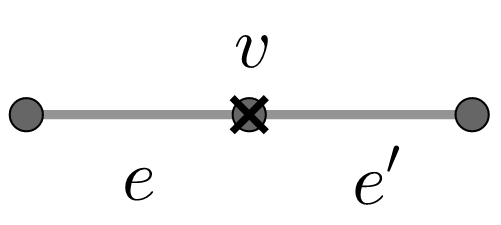
\includegraphics[scale=1.1]{Chaptercflg/media/ineq-deg2-1.png}
    	\caption{A facility is located at $v$}
    	\label{fig:degree2a}
	\end{subfigure}
 	\begin{subfigure}{0.5\textwidth}
    	\centering
    	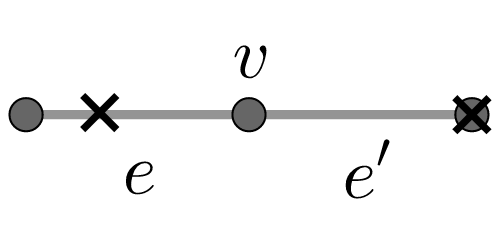
\includegraphics[scale=1.1]{Chaptercflg/media/ineq-deg2-2.png}
    	\caption{Solution with two facilities}
    	\label{fig:degree2b}
	\end{subfigure}
	\caption{Illustration of valid inequalities \eqref{valid-deg2}}
	\label{fig:degree2}
\end{figure}
\Cref{fig:degree2} illustrates the above inequalities. \Cref{fig:degree2a} shows the case in which a facility is located at $v$. Otherwise, if two facilities are placed at $e$ and $e'$ respectively, we can build an equivalent solution by moving one of these facilities to the end node of the corresponding edge that is not $v$, as depicted in \Cref{fig:degree2b}. We recall that the last statement holds due to our Assumption \ref{assumption}.

\subsubsection*{``Neighborhood'' inequalities}
Let us now consider a node $v\in V$, and suppose that there are several facilities placed at different edges in $E(v)$ in a feasible solution. Take $e^*\in E(v)$ containing a facility $f^*$ such that $d(f^*,v)=\min \{d(f,v): f \textup{ is installed at }\:e\in E(v)\}$. The following proposition gives an equivalent feasible solution where the facilities at the edges $e\in E(v)$ such that $e\neq e^*$ are moved to the nodes.
\begin{proposition}\label{lemma:ineq}
Given a node $v \in V$ and an edge $e^* \in E(v)$, for any feasible solution $\hat{y}$ with several facilities placed at edges in $E(v)$, the following solution $y$ is feasible and $\sum_{f \in \cF} y_f \le \sum_{f \in \cF} \hat{y}_f$:
\begin{itemize}
	\item $y_{u}=1$ for all $u\in V$ such that $e=(u,v)\in E(v)$, $e \neq e^*$, and $\hat{y}_e=1$;
	\item $y_{e}=0$ for all $e\in E(v)$ such that $e \neq e^*$, and $\hat{y}_e=1$;
	\item $y_f=\hat{y}_f$ otherwise.
\end{itemize}
\end{proposition}
\begin{proof}
We denote by $N(v)$ the set of vertices adjacent to $v$. Consider the change of facilities from $\hat{y}$ to $y$. The facilities in the edges $E(v) \ \setminus \{e^*\}$ are `pushed' to the vertices $N(v)$. For $u \in N(v)$, if there already exists a facility at $u$, and there is another facility `pushed' to $u$, then these two facilities merge and they are accounted as one facility in  $y$. Hence, the number of facilities of the solution $y$ is at most that of the solution $\hat{y}$.

The proof then consists in showing that $y$ is feasible. We will show that all edges are covered. Let us consider $e\in E$. If $e$ was covered in $\hat{y}$ by facilities not placed at edges in $E(v)$ then it is still covered by these facilities in $y$. Suppose then that a facility placed at $e'\in E(v)$ with $e\neq e^*$ was covering $e$ (or part of $e$) in solution $\hat{y}$, and let $e'=(u,v)$. We distinguish two cases. First, if the facility at $e'$ was partially covering $e$ through node $u$, then it clearly covers at least the same part of $e$ in the new solution $y$ (where the facility is moved to $u$). Otherwise, suppose the facility at $e'$ was partially covering $e$ through node $v$. In this case, the facility at $e^*$ covers at least the same part of $e$ (it is closer to $v$). Since this facility remains unchanged in the new solution, we can guarantee that $e$ is still covered.
\end{proof}
\begin{figure}
	\begin{subfigure}{0.5\textwidth}
    	\centering
    	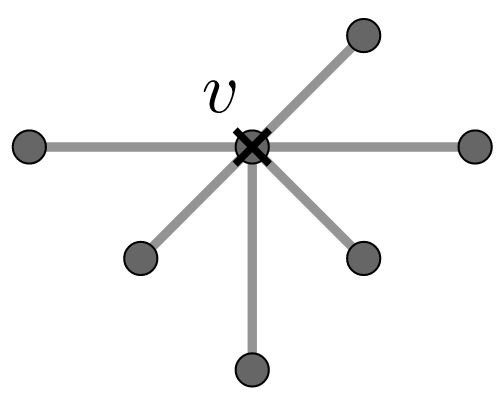
\includegraphics[scale=1.1]{Chaptercflg/media/ineq-general-1.png}
    	\caption{A facility is located at $v$}
    	\label{fig:generala}
	\end{subfigure}
 	\begin{subfigure}{0.5\textwidth}
    	\centering
    	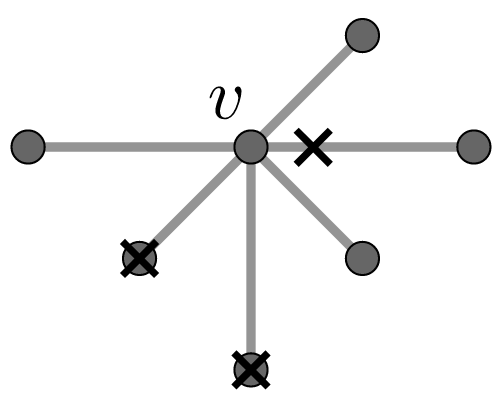
\includegraphics[scale=1.1]{Chaptercflg/media/ineq-general-2.png}
    	\caption{Solution with several facilities}
    	\label{fig:generalb}
	\end{subfigure}
	\caption{Illustration of valid inequalities \eqref{ineq-neigh}}
	\label{fig:general}
\end{figure}
As a consequence of \Cref{lemma:ineq}, the following inequalities are valid:
\begin{equation}
	\sum_{e\in E(v)} y_e \leq 1-y_v \qquad \forall v\in V. \label{ineq-neigh}
\end{equation}
\Cref{fig:general} illustrates the valid inequalities \eqref{ineq-neigh}. In particular, \Cref{fig:generalb} illustrates the equivalent solution given in \Cref{lemma:ineq}. It is easy to observe that these new inequalities are a generalization of inequalities \eqref{valid-deg2}. Moreover, constraints \eqref{ineq-neigh} dominate the model constraints  \eqref{milpa.optimale}--- and are fewer.



\section{Network processing}\label{sec:prepro}
The network processing algorithm analyzes
the network $N$ to compute the parameters and sets needed to construct the MILP model \eqref{milpa}, which we recall next:

\begin{enumerate}
	\item $\cV_{\mathrm{c}}(e)$, $\cE_{\mathrm{c}}(e)$ for all edges $e \in E$;
	\item $\cV_{\mathrm{p}}(v), \cE_{\mathrm{p}}(v), \cEI_{\mathrm{p}}(v)$ for all nodes $v \in V$;
	\item $d(v,v')$ for all pairs of nodes $v,v' \in V$ such that $d(v,v') \le \delta$.
\end{enumerate}

The above data is computed by Algorithms \ref{algo:vcover}, \ref{algo:mutual}  and \ref{algo:graph}. Algorithms \ref{algo:vcover} and \ref{algo:mutual} contain auxiliary functions, which are called within the main Algorithm \ref{algo:graph}. Algorithm \ref{algo:vcover} computes the sets  $\cE(v)$ and $\cV(v)$ (which are not directly used in the MILP but necessary to obtain $\cE_{\mathrm{p}}(v)$ and $\cV_{\mathrm{p}}(v)$), and the distances $d(v,v')$ for all $v,v'\in V$ such that $d(v,v')\leq \delta$. Algorithm \ref{algo:vcover} also computes the sets $\cE_{\mathrm{c}}(v)$,
which will serve as intermediate sets to finally obtain $\cE_{\mathrm{c}}(e)$ in Algorithm \ref{algo:graph}.  The main task in Algorithm \ref{algo:graph} is to compute the sets  $\cV_{\mathrm{c}}(e)$ and $\cE_{\mathrm{c}}(e)$. To that aim, this algorithm calls both Algorithm \ref{algo:vcover} and the procedure ``mutual'' described in Algorithm \ref{algo:mutual}. Once  $\cV_{\mathrm{c}}(e)$ and $\cE_{\mathrm{c}}(e)$ are known, the computation of $\cV_{\mathrm{p}}(v)$ and $\cE_{\mathrm{p}}(v)$ in Algorithm \ref{algo:graph} easily follows by definition.

In the following, we present Algorithm \ref{algo:vcover}, which defines the function ``\ncalgo{}$(N,\delta,s)$''. This function, for each source node $s \in V$, outputs: $\cE_{\mathrm{c}}(s)$, $\cE(s)$,  $\cV(s)$,
and $d(s,v)$ for all $v\in V$ such that $d(s,v)\leq \delta$ (otherwise the algorithm outputs $d(s,v)=+\infty$). The algorithm  starts with empty sets $\cE_{\mathrm{c}}(s), \cE(s), U(s), \cV(s)$, where $U(s)$ is used for intermediate calculations. The set $Q$ denotes nodes whose shortest path (and distance) to $s$ are unknown, and it is initialized to $V$. In the course of the algorithm, $Q$ decreases, while $\cV(s)$ increases. In Lines \ref{algo:vcover.init.dist}-\ref{algo:vcover.start.covers}, the distance $d(s,v)$ and predecessor values $\prev_s(v)$ are initialized, for all $v\in V$. The while loop is an adaptation of the classic Dijkstra algorithm. Line \ref{algo:vcover.remove} selects the node $u$ with the shortest distance to $s$ among all unprocessed nodes, and removes it from $Q$.  If $d(s,u) > \delta$, then none of the remaining nodes in $Q$ are reachable from $s$, and the search is pruned. Otherwise, the neighbors of $u$ that are still in $Q$ are inspected. For each $v\in Q\cap E(u)$, the edge $(u,v)$ is first added to $\cE(s)$. Then, the algorithm computes the length $\ell$ of a path from $s$ to $v$ that traverses $u$. If $\ell < d(s,v)$, then the distance and the predecessor for node $v$ are updated in Lines \ref{algo:vcover.updatedst}- \ref{algo:vcover.updatepred}. In addition, if $\ell < \delta$,  node $v$ and edge $(u,v)$ are added to $\cE_{\mathrm{c}}(s)$ and $\cV(s)$ in Lines \ref{algo:vcover.ccovere} and \ref{algo:vcover.coverv}, respectively.  Otherwise, the edge $e$ is added to the undetermined set $U(s)$. Whether this edge belongs or not to the complete cover set $\cE_{\mathrm{c}}(s)$ is decided later on in the algorithm. Namely,  edges $e=(v_a, v_b)\in U(s)$ are processed in Lines \ref{algo:end1}-\ref{algo:end2}:  if $e$ can be jointly $\delta$-covered  by $s$ from two sides, then $e$ is added to the complete cover $\cE_{\mathrm{c}}(s)$.

Algorithm \ref{algo:mutual} describes the procedure ``\malgo'', which determines, given $e=(v_a,v_b)\in E$ and a candidate edge for the complete cover $e'\in \cE_{\mathrm{c}}(v_a)\cap\cE_{\mathrm{c}}(v_b)$, whether $e' \in \cE_{\mathrm{c}}(e)$. This algorithm is based on \Cref{prop.chara.cEe} in \Cref{sec:prelim}.

Network processing Algorithm \ref{algo:graph} computes all the sets that are needed by the MILP formulation. The algorithm  starts with empty sets $\cE_{\mathrm{c}}(e), \cV_{\mathrm{c}}(e), \cE_{\mathrm{p}}(v), \cV_{\mathrm{p}}(v)$, for $e \in E$ and $v \in V$. In Line \ref{algo:graph.vcomplete}, the algorithm loops through all nodes  $v\in V$ and computes the function ``\ncalgo{}$(N,\delta,v)$'', storing its output. Then, the algorithm calculates the sets $\cV_{\mathrm{c}}(e)$ for $e\in E$, by applying the symmetric relation between these sets and the sets $\cE_{\mathrm{c}}(v)$ from ``\ncalgo{}$(N,\delta,v)$''. After that, in Line \ref{algo:graph.ecomplete}, the algorithm loops through all edges $e=(v_a,v_b) \in E$. It checks whether there is an edge $e' \in \cE_{\mathrm{c}}(v_a) \cap \cE_{\mathrm{c}}(v_b)$ such that $e' \in \cE_{\mathrm{c}}(e)$  (equivalently, $e \in \cE_{\mathrm{c}}(e')$) by calling the procedure "\malgo". Since $e' \in \cE_{\mathrm{c}}(e)$  if and only if $e \in \cE_{\mathrm{c}}(e')$, the loop only runs over pairs such that $e<e'$ (we assume a total order on the elements of $E$).  The loop starting in line \ref{algo:graph.vpartial}, iterates on each node $v \in V$ and looks for $v' \in \cV(v)$ such that there exists an $e \in E(v)$ but $e \notin \cE_{\mathrm{c}}(v')$. The nodes $v'$ found are added to $\cV_{\mathrm{p}}(v)$. Finally, the loop in line \ref{algo:graph.epartial} also iterates on $v\in V$, and looks for $e'=(v'_a,v'_b) \in \cE(v)$ such that there exists $e \in E(v)$ but $e \notin \cE_{\mathrm{c}}(e')$. Each edge found is added to $\cE_{\mathrm{p}}(v)$, and, right after that, the set $\cEI_{\mathrm{p}}(v)$ may be updated after checking the dominance rule described at the end of \Cref{sec:milp}. We have the following complexity result for Algorithm \ref{algo:graph}.

\begin{proposition}
Let $D$ be an upper bound on the degree of the nodes of a connected network $N=(V,E)$.
The time complexity of the network processing Algorithm \ref{algo:graph} is  %${\bO{{|E|^2}+|V|(|E|+ |V|\log |V|)+|V|(|V|+|E|)D}}$.
${\bO{|E|^2+|V||E|(D+\log |V|)}}$.
\end{proposition}
\begin{proof}
%We use the hash function to implement the set data structure such that the time complexity of an operation is $\bO{1}$.

We first analyze the time complexity of the procedure \ncalgo{} described in Algorithm \ref{algo:vcover}. The  main $\textbf{while}$ loop is a modification of the Dijkstra algorithm, and it can be implemented with time complexity ${\bO {(|E|+|V|)\log |V|}}$, see \cite{cormen2009introduction}. Therefore, the overall time complexity of \ncalgo{} is also ${\bO {(|E|+ |V|)\log |V|}}$.

The network processing Algorithm \ref{algo:graph} has four  outer  loops, and next we analyze the complexity of each outer loop.  The first outer loop runs the \ncalgo{} algorithm over the nodes, so its complexity is ${\bO {|V|(|E|+ |V|)\log |V|}}$. The second outer loop  runs the \malgo{} algorithm over the edges pairs, since the mutual algorithm has a constant time complexity, so the complexity of this loop is $\bO{|E|^2}$. The third outer loop is composed of three $\textbf{for}$ loops, and its time complexity is $\bO{D|V|^2}$, which has an upper bound $\bO{D|E||V|}$.  The last outer loop is composed of three $\textbf{for}$ loops, and its time complexity is $\bO{D|E||V|}$.  After summing up the complexity of these loops, we have that the total time complexity of Algorithm \ref{algo:graph} is  ${\bO{|V|((|E|+|V|)\log |V|)+|E|^2+|V||E|D}}$, or, equivalently,
${\bO{|V||E|\log |V|+|E|^2+|V||E|D}}$.

\end{proof}


%%%%%%%%%%%%   alg 1
\begin{algorithm}
\SetAlgoLined
   \textbf{Input:} Network $N= (V, E, ||)$, cover range $\delta > 0$,  a source $s \in V$\;
   \textbf{Output:} $\cE_{\mathrm{c}}(s)$, $\cE(s)$, $\cV(s)$, $d(s,v)$ for all $v\in V$ (returns $d(s,v)=+\infty$ if $d(s,v)>\delta$)\;
   Initialize set $Q \gets V$\;
   Initialize sets $\cE_{\mathrm{c}}(s) \gets \varnothing$, $\cE(s) \gets \varnothing$, $U(s) \gets \varnothing$\;
   Initialize set $\cV(s) \gets \varnothing$\;
	\For{each node $v \in V$}{
    	$d(s,v) \gets +\infty$ \Comment*[r]{Unknown distance from $s$ to $v$} \label{algo:vcover.init.dist}
    	$\prev_{s}(v) \gets  \{\varnothing\}$  \Comment*[r]{Unknown predecessor of $v$} \label{algo:vcover.init.prev}
	}
	$d(s,s) \gets 0$\; %\Comment*[r]{Distance of $s$ to $s$}
	\label{algo:vcover.start.dists}
	add $s$ to $\cV(s)$\; % \Comment*[r]{Node $s$ is covered}
	\label{algo:vcover.start.covers}
	\While{$Q$ is not empty}{
   $u \gets \argmin_{v \in Q} d(s,v)$\;
   remove $u$ from $Q$  \Comment*[r]{Take the closest node $u$ and remove it from $Q$} \label{algo:vcover.remove}
  \If{$d(s,u) > \delta$} {
	$d(s,v) \gets +\infty$ for all $v\in Q$  \Comment*[r]{End of Dijkstra (all nodes in $Q$ are outside the covering radius)}\label{algo:vcover.break}
 	\Break
  }
   \For{each  $v\in Q$ s.t. $v\in E(u)$}{
   $e \gets (u,v)$\;
   add $e$ to $\cE(s)$ \Comment*[r]{Edge $e$ is in the potential cover set of $s$}
   $\ell \gets d(s,u) + l_e$ \Comment*[r]{Path from $s$ to $v$ that traverses $u$}\label{algo:vcover.distfound}
  	\If{ $\ell < d(s,v) $}{ \label{algo:vcover.term}
 	$d(s,v) \gets \ell$  \Comment*[r]{Update the distance to $v$}\label{algo:vcover.updatedst}
 	$\prev_{s}(v) \gets u$  \Comment*[r]{Update the predecessor of $v$}\label{algo:vcover.updatepred}
 	\uIf{ $\ell \le \delta$}{
 	add $e$ to $\cE_{\mathrm{c}}(s)$ \Comment*[r]{Edge $e$ is in the complete cover set of $s$} \label{algo:vcover.ccovere}
	add $v$ to $\cV(s)$  \Comment*[r]{Node $v$ is in the potential cover set of $s$} \label{algo:vcover.coverv}
 	}
 	\Else{
 	add $e$ to $U(s)$ \Comment*[r]{Undetermined edge} \label{algo:vcover.undetermined}
 	}
   }
   }
   }
	\For{each edge $e = (v_a,v_b)$ in $U(s)$ \label{algo:end1} }{
  	\If{$v_a \in \cV(s)$ and $v_b \in \cV(s)$ and $ \delta - d(s,v_a) + \delta - d(s,v_b)  \ge l_e $}{
   	add $e$ to $\cE_{\mathrm{c}}(s)$  \Comment*[r]{Edge $e$ is completely covered} \label{algo:vcover.ccovere2}
  }   
 }\label{algo:end2}

 \caption{single node $\delta$-cover algorithm: \ncalgo{}}
 \label{algo:vcover}
\end{algorithm}


%%%%%%%%%%%%   alg 2
\begin{algorithm}[H]
\SetAlgoLined
   \textbf{Input:} Edges $e=(v_a,v_b),e'=(v'_a,v'_b)$\ such that $e' \in \cE_{\mathrm{c}}(v_a)$ and $e \in \cE_{\mathrm{c}}(v_b)$.\\ %, and the distance function $d$\;
   \textbf{Output:} Boolean value indicating whether $e' \in \cE_{\mathrm{c}}(e)$.\\\
\For{$i \in \{a,b\}$}{
 $Q_{v_ie'} \gets \frac{d(v_i,v'_b)+l_{e'} - d(v_i,v'_a)}{2}$\;  
}
 \For{$i \in \{a,b\}$}{
  \uIf{$q \le Q_{v_ie'}$ } {
 	$r_{v_i}(q) =  \delta - (d({v_i},v'_a) + q)$ \;
  }
  \Else{
  	$r_{v_i}(q) =  \delta- (d({v_i},v'_b)+l_{e'}-q)$ \;
  }
}
 \uIf{$r_{v_a}(Q_{v_ae'})+r_{v_b}(Q_{v_ae'})\ge e$ \textsc{and} $r_{v_a}(Q_{v_be'})+r_{v_b}(Q_{v_be'})\ge e$}{
 \Return \textsc{true}\;
 }
 \Else{
  \Return \textsc{false}\;
 }
 \caption{Edge mutual cover algorithm: \malgo}
 \label{algo:mutual}
\end{algorithm}

%%%%%%%%%%%%   alg 3
\begin{algorithm}[H]
\SetAlgoLined
   \textbf{Input:} Network $N= (V, E, ||)$\, and cover range $\delta > 0$\;
   \textbf{Output:} $\cE_{\mathrm{c}}(e)$, $\cV_{\mathrm{c}}(e)$, $\cE_{\mathrm{p}}(v)$, $\cV_{\mathrm{p}}(v)$, $\cEI_{\mathrm{p}}(v)$, for all $e\in E$ and $v \in V$, and distance function $d$\;
%Initialize the map $d \gets \varnothing$\;
 \For{ each node $v \in V$  \Comment*[r]{Computation of node complete covers $\cV_{\mathrm{c}}(e)$} \label{algo:graph.vcomplete}}{
   $\cE_{\mathrm{c}}(v), \cE(v), \cV(v),d(v,\cdot) \gets \ncalgo{(N, \delta,v)}$ \;
 	\For{each edge $e \in \cE_{\mathrm{c}}(v)$}
   {
   add $v$ to $\cV_{\mathrm{c}}(e)$ \;
   }
 %   \For{each node $v \in \cN(v')$}
   %{  $d(v,v') \gets \dst_{v'}(v)$ \Comment*[r]{Record the distance} }
 }
  \For{ each edge $e = (v_a, v_b) \in E$  \Comment*[r]{Computation of edge complete covers $\cE_{\mathrm{c}}(e)$} \label{algo:graph.ecomplete}}{
  	\For{ each edge $e' = (v'_a, v'_b) \in E$, $e<e'$, such that $e' \in \cE_{\mathrm{c}}(v_a)\cap \cE_{\mathrm{c}}(v_b) $}{
	\uIf{\malgo($e,e',d$)}{
	add $e'$ to $\cE_{\mathrm{c}}(e)$\;
 	add $e$ to $\cE_{\mathrm{c}}(e')$ \;
	}
	}
 }
 \For{each node $v \in V$ \Comment*[r]{Computation of node partial covers $\cV_{\mathrm{p}}(v)$} \label{algo:graph.vpartial}}{
   \For{each node $v' \in \cV(v)$}{
	\For{all $e \in E(v)$}{
	\uIf{$e \notin \cE_{\mathrm{c}}(v')$}{
 	add $v'$ to $\cV_{\mathrm{p}}(v)$\;
 	\Break
	}
	}
 }  
 }
 \For{each node $v \in V$ \Comment*[r]{Computation of edge partial covers $\cE_{\mathrm{p}}(v)$ and $\cEI_{\mathrm{p}}(v)$}  \label{algo:graph.epartial}}{
   \For{each edge $e'=(v'_a,v'_b) \in \cE(v)$}{
	\For{all $e \in E(v)$}{
	\uIf{$e' \notin \cE_{\mathrm{c}}(e)$
	}{
      	add $e'$ to $\cE_{\mathrm{p}}(v)$\;
 	\uIf{$d(v,v'_a)\leq \delta$ \textsc{and}  $d(v,v'_a)\leq d(v,v'_b) + l_{e'}$}{add $(e',a)$ to $\cEI_{\mathrm{p}}(v)$\;}
 	\uIf{$d(v,v'_b)\leq \delta$ \textsc{and}  $d(v,v'_b)\leq d(v,v'_a) + l_{e'}$}{add $(e',b)$ to $\cEI_{\mathrm{p}}(v)$\;}
 	\Break
	}
	}
 }  
 }
 \caption{Network processing algorithm}
 \label{algo:graph}
\end{algorithm}


\section{A reduced formulation for networks with long edges}\label{sec:reduced-milp}
\begin{figure}
	\begin{subfigure}{\textwidth}
    	\centering
    	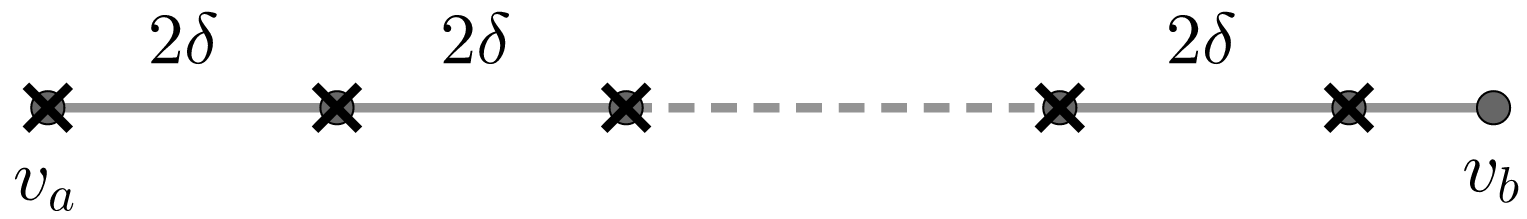
\includegraphics[scale=1.15]{Chaptercflg/media/broken1.png}
    	\caption{A facility is located at $v_a$ ($q_e=0$)}
    	\label{fig:brokena}
	\end{subfigure}
	\vspace{0.25cm}
    
 	\begin{subfigure}{0.45\textwidth}
    	\centering
    	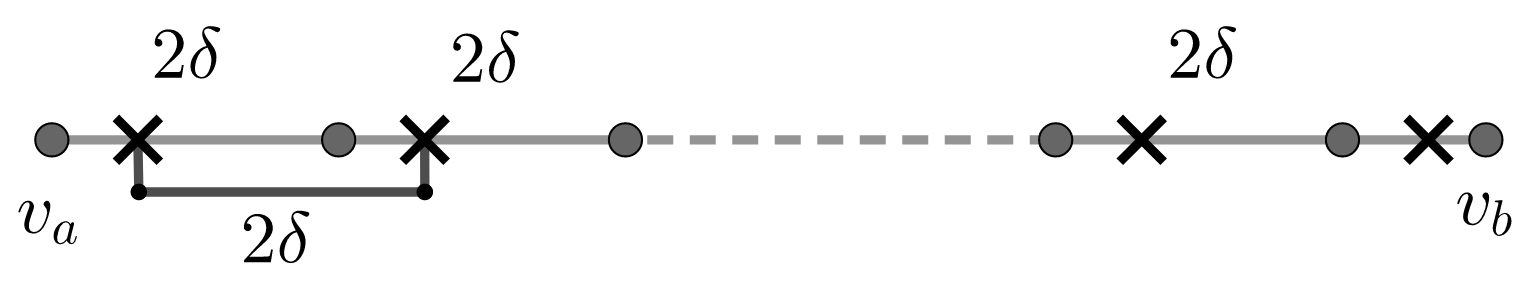
\includegraphics[scale=1.1]{Chaptercflg/media/broken2.png}
    	\caption{A facility is located at the tail ($0<q_e\leq \hat{l}_e$)}
    	\label{fig:brokenb}
	\end{subfigure}
	\begin{subfigure}{0.45\textwidth}
    	\centering
    	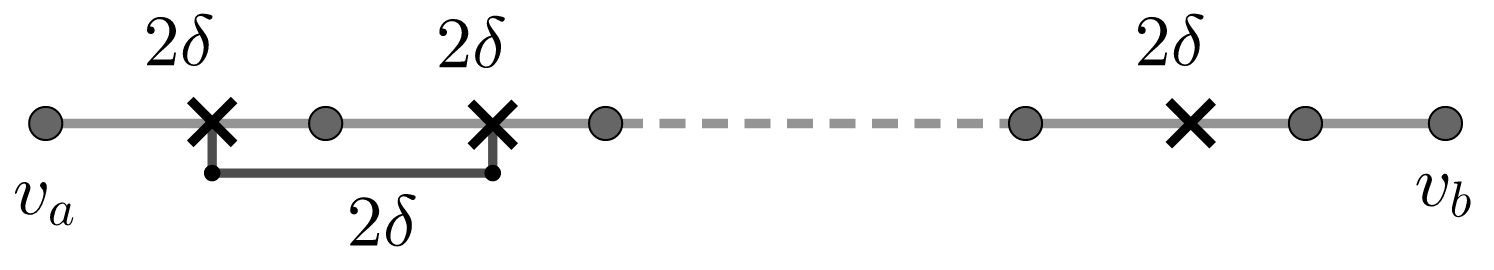
\includegraphics[scale=1.1]{Chaptercflg/media/broken3.png}
    	\caption{No facility is located at the tail ($\hat{l}_e <q_e\leq 2\delta$)}
    	\label{fig:brokenc}
	\end{subfigure}
	\caption{Illustration of \Cref{prop:broken-valid} for a long edge $e$}
	\label{fig:broken}
\end{figure}

The MILP \eqref{milpa} assumes $l_e \le \delta$ for all $e \in E$, however, in many real-world networks, some edge lengths are greater than the covering radius. To reuse the previous results, one approach is to transform a network with long edges into another network with edge lengths at most $\delta$. The transformation is by subdividing edges of the original network into smaller pieces, so the optimal cover does not change. This transformation enables us to apply MILP \eqref{milpa} or the MILP in \cite{Hamacher20} on the transformed network. We note that, in \cite{Hamacher20}, there is a recursive transformation. However, the recursive transformation is not constructive, so we cannot employ it in practice.  Another trivial transformation is by subdividing edges as suggested in \Cref{sec:prelim}.  However, this strategy is a trivial heuristic, and it increases the number of edges and nodes of the transformed network, and thus the number of variables and constraints of the MILP model by a nonlinear factor.

In this section, we present an alternative approach to tackle networks with edge lengths greater than the covering radius. Instead of transforming the network, this approach directly treats long edges in the formulation by using specific sets of constraints and variables. We highlight that the approach is also applicable to ``long paths''. That is, if there is a path in the network whose  intermediate nodes all have degree two, we can represent it by a single edge of length equal to the total length of the path. Indeed, the CSCP does not change after this transformation.
%follows: 1) absorb every degree-2 node into its adjacent edges, resulting in more edges with lengths greater than $\delta$; 2) break each edge with length greater than $\delta$ into new short edges such that their lengths are at most $\delta$.

The main idea of the reduced formulation is to assume a predefined covering of those edges that are long enough. Such covering consists in placing facilities every $2\delta$ distance units on the long edge. Let us consider $e\in E$ such that $l_e> 2\delta$. An edge satisfying this condition is called a \emph{long edge}. We denote by $\hat{l}_e:=l_e-2\delta\lfloor l_e/(2\delta) \rfloor$ the length of the last piece of $e$ after dividing it into pieces of measure $2\delta$. We call  $\hat{l}_e$ the \emph{tail} of $e$.  The following proposition guarantees the correctness of the reduced formulation.

\begin{proposition}\label{prop:broken-valid}
Let $N$ be an undirected network, $e=(v_a,v_b)\in E$ be a long edge, and $\cP '$ be a feasible $\delta$-cover of $N$. Define $\cP$ with $p\in \cP$ for all $p\in \cP ' \setminus e$.  Let $p_e\in \cP '\cap e$ be such that $l(v_a,p_e)=\min_{p'\in \cP '\cap e} l(v_a,p')$, and let $q_e:=l(v_a,p_e)$ (here $q_e$ represents a length, although it will also be a variable of the reduced MILP that we introduce afterward). Note that $q_e\in[0,2\delta]$ (otherwise, $\cP '$ would not be a $\delta$-cover). The set $\cP$ can be completed in such a way that it $\delta$-covers $N$ and $|\cP|\leq | \cP '|$, as follows:
\begin{itemize}
	\item[-] $p_e\in \cP$;
	\item[-] $p\in \cP$ for all $p\in e$, $p>p_e$, such that $l(p_e,p)=2\delta\cdot k$, for some $k\in \mathbb{N}$;
	\item[-] If $\exists p'\in \cP '\cap e$ such that $d(p_e,p')>2\delta\lfloor l(p_e,v_b)/(2\delta) \rfloor$ then $v_b\in \cP $.
\end{itemize}
Moreover, $ \lfloor l_e/(2\delta) \rfloor\leq |\cP \cap e|\leq \lfloor l_e/(2\delta) \rfloor +2$. In particular,
\begin{enumerate}
	\item[(i)] If $0\leq q_e\leq \hat{l}_e$, then  $|\cP \cap e|= \lfloor l_e/(2\delta) \rfloor+1$ if $v_b \notin \cP$,  $|\cP \cap e|= \lfloor l_e/(2\delta) \rfloor+2$ otherwise.
	\item[(ii)] If $\hat{l}_e <q_e\leq 2\delta$, then  $|\cP \cap e|= \lfloor l_e/(2\delta) \rfloor$ if $v_b \notin \cP$,  $|\cP \cap e|= \lfloor l_e/(2\delta) \rfloor+1$ otherwise.
\end{enumerate}
\end{proposition}
\begin{proof}
It is easy to observe that $|\cP|\leq | \cP '|$. First,  since facilities are placed every 2$\delta$ distance on $e$, the original covering $\cP '$ cannot contain fewer facilities than $\cP$. Since the rest of the facilities are just taken from $\cP'$, $|\cP|\leq |\cP '|$. On the other hand, $\cP$ has to $\delta$-cover $N$ for the same reason. That is, the facilities of $\cP$ that were not in $\cP '$ cover at least as much as the ones originally in $\cP'$. The last part of the proposition easily follows from construction, and is illustrated by \Cref{fig:broken}.
\end{proof}

 \begin{remark}
The following example shows that the upper bound is tight, that is, there is a case that satisfies $|\mathcal{P} \cap e| =  \lfloor l_e/(2\delta)  \rfloor +2$. Consider a network with a single edge $e$, and  let $\delta = 1 $ and $l_e = 3.5$. Therefore, to cover $e$, we need 3 facilities $(|\mathcal{P} \cap e |=3)$. Because $\lfloor l_e/(2\delta)  \rfloor +2 = 3$, the upper bound is tight. Similarly, we can give a tight example for the lower bound, by simply setting $l_e= 2$ in the previous  network.
\end{remark}


In the following, we present our reduced formulation, which is an adaptation of MILP \eqref{milpa}. We treat long edges specifically% to subdivide them into smaller edges
, improving the scalability of our approach. Edges $e\in E$ such that $\delta < l_e \leq 2\delta$ are subdivided  into two sub edges of length smaller than $\delta$. Therefore, we assume that, for every $e\in E$, either $l_e\leq \delta$ or $l_e> 2\delta$. In the former case, all the constraints and variables of the model remain unchanged. In the latter, we introduce new variables and constraints to the model, while dropping some of the constraints originally in \eqref{milpa}. The objective function also needs adaptation. We introduce all these modifications next.

Let $e=(v_a,v_b)\in E$ be a long edge and, for any feasible solution, let $q_e$ be as in \Cref{prop:broken-valid}. That is, when $e$ is a long edge, we use the former variable $q_e$ of MILP \eqref{milpa} to represent the position of the left-most facility on $e$ with respect to $v_a$. The placement variables $y_{v_a}$, $y_{v_b}$, and $y_e$ will be used as well, with slightly different meanings to those in \eqref{milpa}, as we will explain later on. We introduce an indicator variable $u_{e}\in\{0,1\}$ to distinguish between two possible ranges in the domain of $q_e$.  If $0 \le q_{e} \le \hat l_e$, then $u_{e} =0$; otherwise $\hat l_{e} \le q_{e} \le 2\delta$ and $u_{e} =1$.  This can be modeled with the following constraints:
\begin{equation}
\label{eq.cvu}
\begin{split}
	q_{e} &\le \hat l_e (1-u_{e})   +2\delta u_{e},\\
	q_{e} &\ge \hat l_e u_{e}. \\
\end{split}
\end{equation}
%The  number of  facilities in $e$ is counted as from the left-most facility in $e_1$ from the last facility in $e_{n-1}$ except for the case that the last one is at $v_n$,
From \Cref{prop:broken-valid},  there is a  transition in the number of facilities on $e$ when $u_{e}$ changes from $0$ to $1$. Let us denote by $L\subseteq E$ the set of long edges of the network. The objective function of the reduced MILP reads as follows
\begin{equation}\label{obj-new}
	\sum_{f\in\cF\setminus L} y_f + \sum_{e\in L} \Big(\left\lceil \frac{l_e}{2\delta}\right\rceil -u_e\Big).
\end{equation}
Note that the coefficients on the last term in the objective already account for the facilities installed at $v_a$ for each $e=(v_a,v_b)\in L$, while they do not do so for $v_b$. This will condition the values of the placement variables in an optimal solution, namely, $y_{v_a}=0$ for all $e=(v_a,v_b)\in L$. The facilities installed at these nodes will be tracked by the variables $q_e$, namely, if $q_e=0$ then a facility would be installed at $v_a$. To complete the modeling of the CSCP, we need to ensure that the covering of the long edge fits into the covering of the rest of the network. Namely, some parts of the network might be covered by facilities placed on $e$, and part of $e$ (namely its tail or the portion between $v_a$ and $p_e$ of \Cref{prop:broken-valid}) could be covered by facilities placed outside $e$.

We focus first on the case $0 \le q_{e} \le  \hat l_{e}$. We need to ensure that both the segment $(v_a,p_e)$ and the tail of $e$ are covered.
%\textbf{Case i):} when , there is a facility in $e_{1}$, the next facility, which
%\begin{itemize}
%	\item does not overlaps its cover with that of $v_1$;
%	\item cover the continuum of $e_l$ between $v_1$ and itself,
%\end{itemize}
%must be placed in $e_2$, and the length between them is $2\delta$, and so on. Then, facilities are placed every $2\delta$ from the first facility in $e_1$, i.e., facilities are located  one per segment from $e_1, e_2,\cdots, e_{n-1}$. The $e_l$ between the first facility and the last facility is covered by $n-1$ facilities, and it remains to check the covering condition for the tail and the head of $e_l$.
For the tail, we know that there is a facility at a distance $\hat l_e-q_{e}$ from $v_b$. This facility covers a length $\delta$ of the remaining fragment on $e$ on its right-hand side, which has a length equal to $ \hat l_{e}-q_{e}$.  The rest of such fragment should be covered, which can be imposed by the following constraint:
  \begin{equation}
  \label{eq.cvu0}
  	r_{v_{b}} \ge \hat l_e-q_{e}-\delta \iff	r_{v_{b}}+q_{e} + \delta \ge \hat l_e \qquad \forall e \in L \mst u_{e} =0.
  \end{equation}
To ensure the covering of the segment $(v_a,p_e)$, we have:
	\begin{equation}
 	r_{v_{a}}+\delta \ge q_{e} \qquad  \forall e \in L \mst u_{e} =0. \nonumber
  \end{equation}
 
 
Let us consider now the case $\hat l_{e} < q_{e} \le 2\delta$.  There is a facility installed at a distance of $2\delta - q_{e} + \hat l_e$ from $v_b$. Then, to ensure that the tail of $e$ is covered, we need to cover the fragment between this facility and $v_b$. Since the facility already covers a length $\delta$ on this fragment, the following constraint enforces the covering of the tail:
%\textbf{Case ii):} when $l_{e_{n-1}} \le q_{e_l} \le 2\delta$, following the same reasoning, facilities are placed every $2\delta$ from the facility in $e_1$. The $e_l$ between the first facility and the last facility is covered by $n-2$ facilities, and it remains to check the covering condition for the tail and the head.  For the tail, there is a facility at $ 2\delta - (q_{e_l} - l_{e_{n-1}})$ to $v_n$, we  need to cover the remaining $$2\delta - (q_{e_l} - l_{e_{n-1}}) = 2\delta + l_{e_{n-1}}  - q_{e_l}$$ length:
  \begin{equation}
  \label{eq.cvu1}
  	r_{v_{b}}\ge 2\delta  - q_{e}+ \hat l_{e}  -\delta   \iff  r_{v_{b}}+q_{e} - \delta \ge\hat l_{e}   \qquad\forall e \in L \mst u_{e} =1.
  \end{equation}
To ensure the covering of the segment $(v_a,p_e)$, we have the same equation as before:
	\begin{equation}
 	r_{v_{a}}+\delta \ge q_{e} \qquad  \forall e \in L \mst u_{e} =1. \nonumber
  \end{equation}

In summary, the following constraints ensure that the edge $e$ is fully covered:
\begin{eqnarray}
	r_{v_{a}}+\delta \ge q_{e} & \forall e\in L,\label{eq.cvhead}\\
	r_{v_{b}} + q_{e} - (2u_{e}-1)\delta \ge \hat l_e & \forall e\in L.\label{eq.cvtail}
\end{eqnarray}
Constraint \eqref{eq.cvtail} gathers \eqref{eq.cvu0} and \eqref{eq.cvu1} in a single constraint. The reduced MILP model is as follows (we avoid extended writing of the model for the sake of conciseness):
\begin{eqnarray}
	\min & \eqref{obj-new} \nonumber\\
	\mst   & \eqref{milpa.completecover1}, \eqref{milpa.completecover2}, \eqref{milpa.covere} & e\notin L \nonumber\\
	& \eqref{milpa.optimale}, \eqref{milpa.coord},\eqref{milpa.indicatorei} & e'\notin L \nonumber\\
	&  \eqref{milpa.enforcex1}, \eqref{milpa.enforcex2}, \eqref{milpa.lcoversos},\eqref{milpa.indicatorv},\eqref{milpa.wbdl},\eqref{milpa.coverdist-node},\eqref{milpa.coverdist-edge}, \eqref{milpa.varyw},\eqref{milpa.varindicator},\eqref{milpa.varcontinuous}\nonumber\\
	& \eqref{eq.cvu}, \eqref{eq.cvhead}, \eqref{eq.cvtail} \nonumber\\
	& y_{e}=1 & e \in L \label{fix-y}\\
	& w_{e}=0 & e \in L, \label{fix-w}
\end{eqnarray}
 where, if $e\in L$, the term $\tau_{vei}(q_{e})$ in \eqref{milpa.coverdist-edge} is replaced by $d(v,v_{i})+ \mathbf{1}_{i=a}q_{e} +\mathbf{1}_{i=b}(2\delta u_{e} + \hat{l}_e  - q_{e})$.
 We enforce \eqref{fix-y} because $e$ always contains a facility if $e\in L$. On the other hand, we need to include constraints \eqref{fix-w} to guarantee that the variables $r_{v_a}$ and $r_{v_b}$ can take positive values. Indeed, if $w_e=1$ for $e\in L$, it may happen that $x_{v_a}=1$ or $x_{v_b}=1$, which will will imply, respectively,  $r_{v_a}=0$ or $r_{v_b}=0$  due to \eqref{milpa.wbdl}.
%Now we can adapt the MILP model for the long edge $e_l$ as follows:
%\begin{enumerate}
%\item its objective coefficient is $n-1 - u_{e_l}$;
%\item its placement variable is $y_{e_l}$, and coordinate variable is $q_{e_l} \in [0, 2\delta]$.
%\end{enumerate}
We compute the complete and partial cover sets in the same way as  for the original MILP model. Note that no edge or node can completely cover $e$ if $e\in L$.


The following theorem is on the scalability of the reduced MILP above.
\begin{theorem}
Given a network %$N=(V,E,\rho l)$ for a scalar $\rho \ge 1$,
$N=(V,E,l)$, the maximum number of variables and constraints of the reduced MILP model only depends on $V$ and $E$.% and $l$.
\end{theorem}
\begin{proof}
The number of constraints and variables of the reduced model does not grow with the edge lengths, except for a constant factor of 2 for those edges $e\in E$ such that $\delta < l_e \leq 2\delta$.
\end{proof}

\section{Computational results}\label{sec:compu}

In this section, we present the computational experiments testing the existing and proposed formulations and strengthening techniques for  CSCP and its discrete variant (facilities on nodes).

\subsection{Experiment Setup}
We describe the setup of the experiments including the benchmarks, development environment, implementation of algorithms and solution statistics. The  computational results and source code are publicly released on our project website: \href{https://github.com/lidingxu/cflg/}{https://github.com/lidingxu/cflg/}, where we provide a bash file to reproduce the experiments in Linux systems. Those benchmarks that we generated for this study, or that were publicly available already, are also available at the repository. %Using a single command to run this bash file, all experiment results can be reproduced.

\textbf{Benchmarks.}
We use three different benchmarking sets: two come from the literature, and the other has been generated synthetically. For every instance, we set the coverage radius $\delta$ equal to the  average of the edge lengths. We describe these benchmarks next.

\texttt{Kgroup.} It consists of 23 prize-collecting Steiner tree problem instances from \cite{Ljubic2006}, and the benchmark includes the graphs and edge lengths of these instances. These random geometric instances are designed to have a local structure somewhat similar to street maps. Nodes correspond to random points in the unit square. The number of nodes ranges from 22 to 241. There
is an edge between two nodes if their distance is no more than a prescribed threshold which depends on the number of nodes, and the length of an edge is the Euclidean distance between the two points. It is divided into two sets, \texttt{Kgroup\_A} and  \texttt{Kgroup\_B}. The first one consists of 12 small instances with up to 45 nodes, and the second one consists of 11 large instances with up to 241 nodes.  

\texttt{City.} It consists of real data of 9  street networks for some German cities, and it was first used in \cite{Kalsics}.  The number of nodes ranges from 132 to 771. The length of each edge is the length of the underlying street segment.

\texttt{Random.} It consists of 24  random network instances generated via Erdős-Rényi binomial method with the package ``Networkx" (see \cite{SciPyProceedings_11}).  A network is constructed by connecting nodes randomly. Each edge is included with a predefined uniform probability $p$. The number of nodes, $n$, is in $\{10, 15, 20, 25, 30, 40\}$. For each $n$, we generate random graphs with different adjacency probabilities, namely  $p \in \{0.1, 0.2, 0.3, 0.4\}$. Furthermore, we split these instances into two benchmarks: \texttt{Random\_A} and \texttt{Random\_B}.  \texttt{Random\_A} contains instances with $n \in \{10,15,20\}$.   \texttt{Random\_B} contains instances with $n \in \{25,30.40\}$. \\



\textbf{Coverage radii.}
For each network, we define two sets of coverage radii: ``Small'' equal to [Average Edge
Length], and ``Large'' equal to ×2 [Average Edge Length], respectively.
\\

%%or $2 \times$ [avg. edge length] (Large). Therefore, we create two problem sets for each benchmark, and we label the coverage mode as the suffix of an instance or a benchmark. For example, \texttt{City-Small} is the problem set of \texttt{City} benchmark with a small coverage.\\

\textbf{Problem preprocessing.}
Networks of instances are modified in a problem preprocessing step to be amenable to MILP models.

 Given an original network of each instance, in the first preprocessing step, we delete any degree-two node and concatenate its adjacent edges to a new edge, as long as the deletion does not yield a self-loop. Such a node can be treated as an interior point of the new edge. We refer to the preprocessed network without any such degree-two node as the degree-two-free network.


Even after the first preprocessing step,
 the degree-two-free network may not correspond to the actual problem network to solve, since we may subdivide the degree-two-free network for the non-reduced model to guarantee that $\delta > \max_{e \in E} |e|$. We refer to the preprocessed network after the second preprocessing step as the subdivided network, which is degree-two-free and satisfies $\delta > \max_{e \in E} |e|$.
 Therefore, the size (number of nodes and edges) of a subdivided network depends on $\delta$.\\


\textbf{Development environment.}
The experiments are conducted on a computer with Intel Core i7-6700K  CPU @ 4.00GHZ and 16GB main memory. JuMP \cite{DunningHuchetteLubin2017} is a modeling language for mathematical optimization embedded in Julia. We use JuMP  to implement our models and interact with MILP solvers. Specifically, we use ILOG CPLEX 20.1 to solve our models. Alternatively, the implementation allows users to switch easily to other solvers (e.g. Gurobi and GLPK).

CPLEX's parameters are set as their defaults, except that we disable its parallelism and set  the MIP absolute gap to 1 (due to the integral objective). The experiments are partitioned into jobs. Every job calls CPLEX to solve an instance, and this job is handled by one process of the multi-core CPU. To safeguard
against a potential mutual slowdown of parallel processes, we run only one job per core at a
time, and we use at most three processes in parallelism.  The time limit of each job is set to 1800 CPU seconds.\\

\textbf{Model implementation.}
We implement six models based on different combinations of formulations and settings. The first five models address CSCP, while the last model solves its discrete restriction, i.e. the variant in which facilities must be placed at nodes. These models are as follows.

\texttt{EF.} This model implements the model from \cite{Hamacher20} for CSCP. This formulation only uses edges to model facility locations, and the authors do not consider the complete and partial cover sets to delimit the size of the model. This model assumes $\delta > \max_{e \in E}|e|$, and it reads the subdivided graph.

\texttt{F0.} This model implements a  basic formulation that is a simplification of the model \eqref{milpa}. It does not use the complete and partial cover information nor any of the strengthening techniques in \Cref{sec:strenght}. Hence, it does not call the network processing algorithm \ncalgo. This model assumes $\delta > \max_{e \in E}|e|$, and it reads the subdivided graph. More precisely, the constraints \eqref{milpa.completecover1}-\eqref{milpa.enforcex2} related to complete covers are removed, the complete cover variables $w$ are fixed to $0$; for each $v \in V$, the partial cover sets $\cE_{\mathrm{p}}(v)$, $\cEI_{\mathrm{p}}(v)$ are solely set, respectively, as $E$ and $E \times \{a,b\}$, and consequently, $M_{v} = \delta$, $M_{vv'} = r(N)$ for $v' \in \cE_{\mathrm{p}}(v)$, $M_{ve'i'} = r(N) + |e'|$ for $(e',i') \in \cEI_{\mathrm{p}}(v)$ are trivial valid bound constants, where $r(N):= \max_{v,v' \in N} d(v,v')$ is the radius of the problem network $N$.

\texttt{F.}  This model implements the complete formulation \eqref{milpa} for CSCP, it does use the complete and partial cover information, and hence it  calls the network processing algorithm \ncalgo.  It does not use the strengthening techniques in \Cref{sec:strenght}. This model assumes $\delta > \max_{e \in E}|e|$, and it reads the subdivided network as well.  For each $v \in V$, due to the delimited partial cover set,  $M_{v} = \delta$, $M_{vv'} = \delta$ for $v' \in \cE_{\mathrm{p}}(v)$, $M_{ve'i'} = \delta + |e'|$ for $(e',i') \in \cEI_{\mathrm{p}}(v)$ are valid bound constants.

\texttt{SF.} This model strengthens  $\texttt{F}$ by using the techniques described in \Cref{sec:strenght}. %This model assumes $\delta > \max_{e \in E}|e|$, and it reads the subdivided graph as well.
More precisely, the big-M constants are reduced as \Cref{sec:strenght.bd}; the "Leafs" inequalities are used to fix variables; and the "Neighborhood" inequalities are implemented as model constraints which replace \eqref{milpa.optimale}.

\texttt{RF.} This model implements the reduced formulation from \Cref{sec:reduced-milp}. It only requires $\delta < 2\max_{e \in E}|e|$. Given a degree-two-free network, it models the long edge specifically as the description \Cref{sec:reduced-milp}, and it subdivides the edges with lengths greater than $\delta$ and smaller than $2\delta$ into two sub-edges.

\texttt{SFD.}  Any solution of the discrete restriction of CSCP---where facilities can only be placed at nodes--- is a feasible solution of CSCP. We name this discrete restriction by the \dfproblem.  This model solves the \dfproblem, which solely sets $y_e = 0$ for all $e \in E$ in \texttt{SF} model.

The above models are summarized in \Cref{tab.modsum}. Both \texttt{EF} and \texttt{F0} consider that any two points in the network can possibly cover each other, and do not utilize the complete and partial cover information. They have been already compared in \Cref{sec:comp}, and hence \texttt{F0} should have fewer variables and constraints than \texttt{EF}. We are interested in the dual gaps obtained after the models are solved within the time limit for these models.
 
 \begin{table}[]
 \resizebox{0.99\columnwidth}{!}{
\begin{tabular}{|l|lllllll|}
\hline
  \multicolumn{1}{|l|}{Model}   & \multicolumn{1}{l|}{Problem} & \multicolumn{1}{l|}{Delimitation} & \multicolumn{1}{l|}{Strengthening} & \multicolumn{1}{l|}{Long edge} & \multicolumn{1}{l|}{Size} & \multicolumn{1}{l|}{Input network} & \multicolumn{1}{l|}{Comment} \\ \hline
\texttt{EF}  & CSCP                                  	& No                                	& No                              	& No                         	& Very large                  	& Subdivided network             	&            	From \cite{Hamacher20}          	\\ \cline{1-8}
\texttt{F0}  &  CSCP                                    	& No                                	& No                              	& No                         	& Large                       	& Subdivided network             	& The simple model          	\\ \cline{1-8}
\texttt{F}   &  CSCP                                    	& Yes                               	& No                              	& No                         	& Medium                      	& Subdivided network             	& The complete model       	\\ \cline{1-8}
\texttt{SF}  &  CSCP                                    	& Yes                               	& Yes                             	& No                         	& Medium                      	& Subdivided network             	& The strengthened model   	\\ \cline{1-8}
\texttt{RF}  &  CSCP                                    	& Yes                               	& Yes                             	& Yes                        	& Small                       	& Degree-two-free network        	& The reduced model        	\\ \cline{1-8}
\texttt{SFD} &  \dfproblem                                    	& Yes                               	& Yes                             	& No                         	& Very Small                  	& Subdivided network             	& The discrete model       	\\ \cline{1-8}
\end{tabular}}
\caption{Model summary}
\label{tab.modsum}
\end{table}
 


 
\textbf{Performance metrics and statistical tests.}
We describe the performance metrics and the ways to compute  their statistics. These statistics will be used to evaluate the model performance.

Let $\underline{v}$ be a dual lower bound and $\overline{v}$ be a primal upper bound obtained after solving some of the models described above,  the relative dual gap   is defined as:
\begin{equation*}
   \sigma := \frac{\overline{v} - \underline{v}}{\overline{v}}.
\end{equation*}
A smaller relative dual gap indicates better primal and dual behavior of the model.
 
Let $n_{sd}$ be the number of nodes of the subdivided network of that instance, note that  a trivial primal solution is the set of the nodes of the subdivided network (for which edge length is at most $\delta$). Therefore, to normalize the primal solution value, we define the relative primal bound  $$v_r := \frac{\overline{v}}{n_{sd}} .$$ If $v_r < 1$, then the model finds a solution better than the trivial one.


In order to evaluate model performance, we compute shifted geometric means (SGMs) of performance metrics, which provides a
measure for relative differences. This avoids statistics from being dominated by outliers with
large absolute values as is the case for the arithmetic mean. The SGM also avoids an over-representation of results with small absolute values.  The SGM of values $v_1,...,v_M \geq 0$ with shift $s \geq 0$ is defined
as
\begin{equation*}
  \left(\prod_{i=1}^M (v_i + s)\right)^{1/M} - s.
\end{equation*}


We say an instance is affected by a model, if solving this model finds a feasible solution; the instance is solved by this model, if solving this model finds an optimal solution. If an instance is unaffected, usually the model is too large to be read into the MILP solver.


We record the following performance metrics of each instance for each model, and compute the benchmark-wise SGMs:

 
\begin{enumerate}
	\item $t$: the total running time in CPU seconds, with a shifted value set to 1 second;
    
   \item $\sigma$: the relative dual gap, with a shifted value set to $0.01$;
  	\item $v_r$: the relative primal bound, with a shifted value set to $0.01$.
	 
\end{enumerate}
For an unaffected instance, we set by default $t= 1800$, $\sigma = 1$ and $v_r = 1$. Note that the time does not include the preprocessing time, since we find that the preprocessing is usually at most 0.5 seconds. \\

We will discuss the computational results, which are divided into two parts. In the first part, we compare the five models \texttt{EF}, \texttt{F0}, \texttt{F}, \texttt{SF}, and \texttt{RF}. We evaluate the performance metrics of these models. The second part compares \texttt{RF}  and \texttt{SFD},  quantifying the facilities that are saved by allowing continuous location. In the following, we will analyze the aggregated results. 

\subsection{Comparative Analysis of Continuous Models}



We compare five continuous models for the CSCP, namely  \texttt{EF}, \texttt{F0}, \texttt{F}, \texttt{SF}, and \texttt{RF}. For each  benchmark, radius and model, we record a triple of integers S/A/T: S denotes the number of solved instances, A denotes the number of affected instances, and T denotes the number of total instances in the benchmark. Moreover, we also report the  average SGMs of the dual gaps, solving times and relative primal bounds among all instances in the benchmark. \Cref{tab.cm} summarizes these results.
 
 First, we notice that \texttt{EF} cannot affect any instance in any benchmark; \texttt{RF}, \texttt{SF} and \texttt{RF} can affect all instances, i.e., solutions are provided by these models; \texttt{RF} is the model that solves the most number of instances (11), and \texttt{SF} is the second best one (10).
 
 Secondly, we compare \texttt{EF} and \texttt{F0}. \texttt{F0} is obviously superior to \texttt{EF}. With \texttt{F0}, 39 among 56 instances of small radius (resp. 42 among 56 instances of large radius) can be read by the CPLEX solver, while the instances modeled by \texttt{EF} are too large to read. Therefore, better solutions than trivial solutions are found by \texttt{F0}: on average, for instance of small radius (resp. large radius), \texttt{F0} finds solutions that use $25.2\%$ (resp. $74.1\%$) fewer facilities than the trivial solution.

Then, we compare \texttt{F0}, \texttt{F}  and \texttt{SF}. With the delimitation of complete and partial covering sets, \texttt{F} and \texttt{SF} can affect all instances (especially those in \texttt{Kgroup\_B}, of which \texttt{F0} could just read one).
With the strengthening technique, \texttt{SF} has only marginal improvement in the relative primal bound, and solving time, while \texttt{F} is even slightly better than \texttt{SF} in the dual gap. We observe, in our experiment, that adding valid inequalities might slow down the internal solving process of CPLEX.

Finally, we compare  \texttt{SF} and \texttt{RF}. \texttt{RF} outperforms \texttt{SF} in all performance metrics. Moreover,  \texttt{RF} is the best one among those models affecting all instances. Indeed, for many instances, their degree-two-free networks may contain long edges, and \texttt{RF} avoids introducing too many variables and constraints for modeling their coverage.

\texttt{Kgroup\_B} is the hardest benchmark. The best model \texttt{RF} still has  an average dual gap of $59.1\%$ and $154.2\%$ relative primal bound for instances of small radius, and this means that $\texttt{RF}$ cannot produce better solutions than the trivial one.

We find that for all the models (except for \texttt{EF}), the average dual gaps and solving times of instances of large radius are smaller than those of instances of small radius. This shows that the large radius has a positive effect on the model performance, and an instance of a small radius may be more difficult than the same instance of a large radius. This is because, with a larger radius, the network after processing is smaller.

In \Cref{fig.scatter5}, we show scatter plots of the relative dual gaps and the relative primal bounds  of affected instances between different settings. For every plot, there is a line in which the points have equal (X,Y)-values. If points fall below the line, then the Y-axis model performs better for the corresponding instances. Note that when comparing  \texttt{F0} and  \texttt{F}, the plots do not consider the unaffected instances of \texttt{F0} which are affected or solved by \texttt{F}. Moreover, \texttt{F0} even closes more duality gaps than \texttt{F}, but \texttt{F} can find better primal solutions. These plots give an overview of all affected instances and support the above analysis.

%In summary, we have compared five models, and we conclude that the sizes of models are the main barriers to their scalability.
To summarize, we have shown that the two proposed techniques---  that to delimit the coverage  areas from a given point in \Cref{sec:prelim}, and that to cover long edges in \Cref{sec:reduced-milp},--- can reduce the model size drastically. Among the five models tested, $\texttt{RF}$ features the best overall performance, which is achieved by directly modeling covers on long edges. On the other hand, delimiting the covering sets to the potential, complete and partial covers also reduce the model size, which allows $\texttt{F}$ to read all the tested instances.




\begin{table}[]
\centering
\scalebox{0.85}{
\begin{tabular}{|l|l|*{4}{r}|*{4}{r}}
\hline
\multirow{2}{*}{Benchmark} & \multirow{2}{*}{Radius} & \multicolumn{4}{l|}{\texttt{EF}}                                                                                 	& \multicolumn{4}{l|}{\texttt{F0}}                                                                                                    	\\ \cline{3-10}
                       	& & \multicolumn{1}{l|}{time} & \multicolumn{1}{l|}{$\sigma(\%)$} & \multicolumn{1}{l|}{$v_r(\%)$} & \multicolumn{1}{l|}{S/A/T} & \multicolumn{1}{l|}{time} & \multicolumn{1}{l|}{$\sigma(\%)$} & \multicolumn{1}{l|}{$v_r(\%)$} & \multicolumn{1}{l|}{S/A/T}  \\ \hline
	\multirow{2}{*}{\texttt{city}}&Small & 1800.0 & 100.0\% & 100.0\% & 0/0/9 & 1801.7 & 56.8\% & 83.3\% & \multicolumn{1}{l|}{0/3/9} \\
&Large & 1800.0 & 100.0\% & 100.0\% & 0/0/9 & 1800.9 & 42.3\% & 36.2\% & \multicolumn{1}{l|}{0/6/9} \\ \cline{1-1}
\multirow{2}{*}{\texttt{Kgroup\_A}}&Small & 1800.0 & 100.0\% & 100.0\% & 0/0/11 & 1802.6 & 25.1\% & 85.0\% & \multicolumn{1}{l|}{0/11/11} \\
&Large & 1800.0 & 100.0\% & 100.0\% & 0/0/11 & 139.2 & 14.7\% & 19.2\% & \multicolumn{1}{l|}{7/11/11} \\ \cline{1-1}
\multirow{2}{*}{\texttt{Kgroup\_B}}&Small & 1800.0 & 100.0\% & 100.0\% & 0/0/12 & 1800.4 & 92.6\% & 98.8\% & \multicolumn{1}{l|}{0/1/12} \\
&Large & 1800.0 & 100.0\% & 100.0\% & 0/0/12 & 1800.1 & 93.2\% & 86.6\% & \multicolumn{1}{l|}{0/1/12} \\ \cline{1-1}
\multirow{2}{*}{\texttt{random\_A}}&Small & 1800.0 & 100.0\% & 100.0\% & 0/0/12 & 16.8 & 15.9\% & 54.8\% & \multicolumn{1}{l|}{9/12/12} \\
&Large & 1800.0 & 100.0\% & 100.0\% & 0/0/12 & 0.2 & 25.5\% & 19.5\% & \multicolumn{1}{l|}{12/12/12} \\ \cline{1-1}
\multirow{2}{*}{\texttt{random\_B}}&Small & 1800.0 & 100.0\% & 100.0\% & 0/0/12 & 1317.6 & 36.4\% & 63.3\% & \multicolumn{1}{l|}{1/12/12} \\
&Large & 1800.0 & 100.0\% & 100.0\% & 0/0/12 & 154.4 & 26.0\% & 10.0\% & \multicolumn{1}{l|}{11/12/12} \\ \cline{1-10}
\multirow{2}{*}{\texttt{all}}&Small & 1800.0 & 100.0\% & 100.0\% & 0/0/56 & 625.8 & 37.4\% & 74.8\% & \multicolumn{1}{l|}{10/39/56} \\
&Large & 1800.0 & 100.0\% & 100.0\% & 0/0/56 & 132.5 & 33.1\% & 25.9\% & \multicolumn{1}{l|}{30/42/56} \\
 \cline{1-10}
\multicolumn{10}{c}{}\\
\cline{1-10}
\multirow{2}{*}{Benchmark} & \multirow{2}{*}{Radius} & \multicolumn{4}{l|}{\texttt{F}}                                                                                 	& \multicolumn{4}{l|}{\texttt{SF}}                                                                                                    	\\ \cline{3-10}
                       	& & \multicolumn{1}{l|}{time} & \multicolumn{1}{l|}{$\sigma(\%)$} & \multicolumn{1}{l|}{$v_r(\%)$} & \multicolumn{1}{l|}{S/A/T} & \multicolumn{1}{l|}{time} & \multicolumn{1}{l|}{$\sigma(\%)$} & \multicolumn{1}{l|}{$v_r(\%)$} & \multicolumn{1}{l|}{S/A/T}  \\ \hline
\multirow{2}{*}{\texttt{city}}&Small & 1802.9 & 29.5\% & 62.2\% & 0/9/9 & 1801.3 & 30.1\% & 66.9\% & \multicolumn{1}{l|}{0/9/9} \\
&Large & 1801.2 & 28.4\% & 21.7\% & 0/9/9 & 1800.9 & 29.1\% & 21.7\% & \multicolumn{1}{l|}{0/9/9} \\  \cline{1-1}
\multirow{2}{*}{\texttt{Kgroup\_A}}&Small & 1803.0 & 33.1\% & 82.2\% & 0/11/11 & 1801.3 & 32.0\% & 80.6\% & \multicolumn{1}{l|}{0/11/11} \\
&Large & 238.0 & 18.9\% & 19.1\% & 8/11/11 & 300.8 & 19.0\% & 19.1\% & \multicolumn{1}{l|}{8/11/11} \\  \cline{1-1}
\multirow{2}{*}{\texttt{Kgroup\_B}}&Small & 1800.6 & 80.8\% & 240.5\% & 0/12/12 & 1801.4 & 79.7\% & 191.9\% & \multicolumn{1}{l|}{0/12/12} \\
&Large & 1800.4 & 85.1\% & 80.5\% & 0/12/12 & 1800.7 & 85.9\% & 77.3\% & \multicolumn{1}{l|}{0/12/12} \\  \cline{1-1}
\multirow{2}{*}{\texttt{random\_A}}&Small & 20.2 & 16.5\% & 54.3\% & 9/12/12 & 16.1 & 17.1\% & 54.9\% & \multicolumn{1}{l|}{9/12/12} \\
&Large & 0.3 & 25.5\% & 19.5\% & 12/12/12 & 0.2 & 10.4\% & 17.9\% & \multicolumn{1}{l|}{12/12/12} \\  \cline{1-1}
\multirow{2}{*}{\texttt{random\_B}}&Small & 1574.2 & 38.8\% & 64.9\% & 1/12/12 & 1501.2 & 40.0\% & 67.5\% & \multicolumn{1}{l|}{1/12/12} \\
&Large & 220.5 & 19.9\% & 10.3\% & 9/12/12 & 175.7 & 18.8\% & 10.0\% & \multicolumn{1}{l|}{11/12/12} \\  \cline{1-10}
\multirow{2}{*}{\texttt{all}}&Small & 675.0 & 35.2\% & 86.2\% & 10/56/56 & 637.6 & 35.5\% & 83.6\% & \multicolumn{1}{l|}{10/56/56} \\
&Large & 163.0 & 30.2\% & 23.6\% & 29/56/56 & 160.9 & 24.9\% & 22.8\% & \multicolumn{1}{l|}{31/56/56} \\

\cline{1-10}
\multicolumn{10}{c}{}\\
\cline{1-6}

\multirow{2}{*}{Benchmark} & \multirow{2}{*}{Radius}  & \multicolumn{4}{l|}{\texttt{RF}}                                                                                 	& \multicolumn{4}{l}{}                                                                                                    	\\ \cline{3-6}
                  	&  	& \multicolumn{1}{l|}{time} & \multicolumn{1}{l|}{$\sigma(\%)$} & \multicolumn{1}{l|}{$v_r(\%)$} & \multicolumn{1}{l|}{S/A/T} & \multicolumn{1}{l}{} & \multicolumn{1}{l}{} & \multicolumn{1}{l}{} & \multicolumn{1}{l}{}  \\ \cline{1-6}
\multirow{2}{*}{\texttt{city}}&Small & 1804.4 & 16.2\% & 54.1\% & \multicolumn{1}{l|}{0/9/9} \\
&Large & 1801.5 & 25.8\% & 21.3\% & \multicolumn{1}{l|}{0/9/9} \\  \cline{1-1}
\multirow{2}{*}{\texttt{Kgroup\_A}}&Small & 1622.6 & 21.5\% & 77.5\% & \multicolumn{1}{l|}{1/11/11} \\
&Large & 158.9 & 19.2\% & 19.3\% & \multicolumn{1}{l|}{8/11/11} \\  \cline{1-1}
\multirow{2}{*}{\texttt{Kgroup\_B}}&Small & 1800.9 & 59.1\% & 154.2\% & \multicolumn{1}{l|}{0/12/12} \\
&Large & 1800.6 & 75.5\% & 63.3\% & \multicolumn{1}{l|}{0/12/12} \\  \cline{1-1}
\multirow{2}{*}{\texttt{random\_A}}&Small & 15.9 & 8.1\% & 54.3\% & \multicolumn{1}{l|}{9/12/12} \\
&Large & 0.3 & 26.6\% & 19.8\% & \multicolumn{1}{l|}{12/12/12} \\  \cline{1-1}
\multirow{2}{*}{\texttt{random\_B}}&Small & 1304.3 & 38.5\% & 63.8\% & \multicolumn{1}{l|}{1/12/12} \\
&Large & 190.2 & 19.8\% & 11.2\% & \multicolumn{1}{l|}{9/12/12} \\  \cline{1-6}
\multirow{2}{*}{\texttt{all}}&Small & 604.9 & 23.7\% & 75.4\% & \multicolumn{1}{l|}{11/56/56} \\
&Large & 146.6 & 29.2\% & 22.8\% & \multicolumn{1}{l|}{29/56/56} \\
\cline{1-6}
\end{tabular}
}

\caption{Results for continuous models} \label{tab.cm}
\end{table}



 \begin{figure}[!h]
\centering{
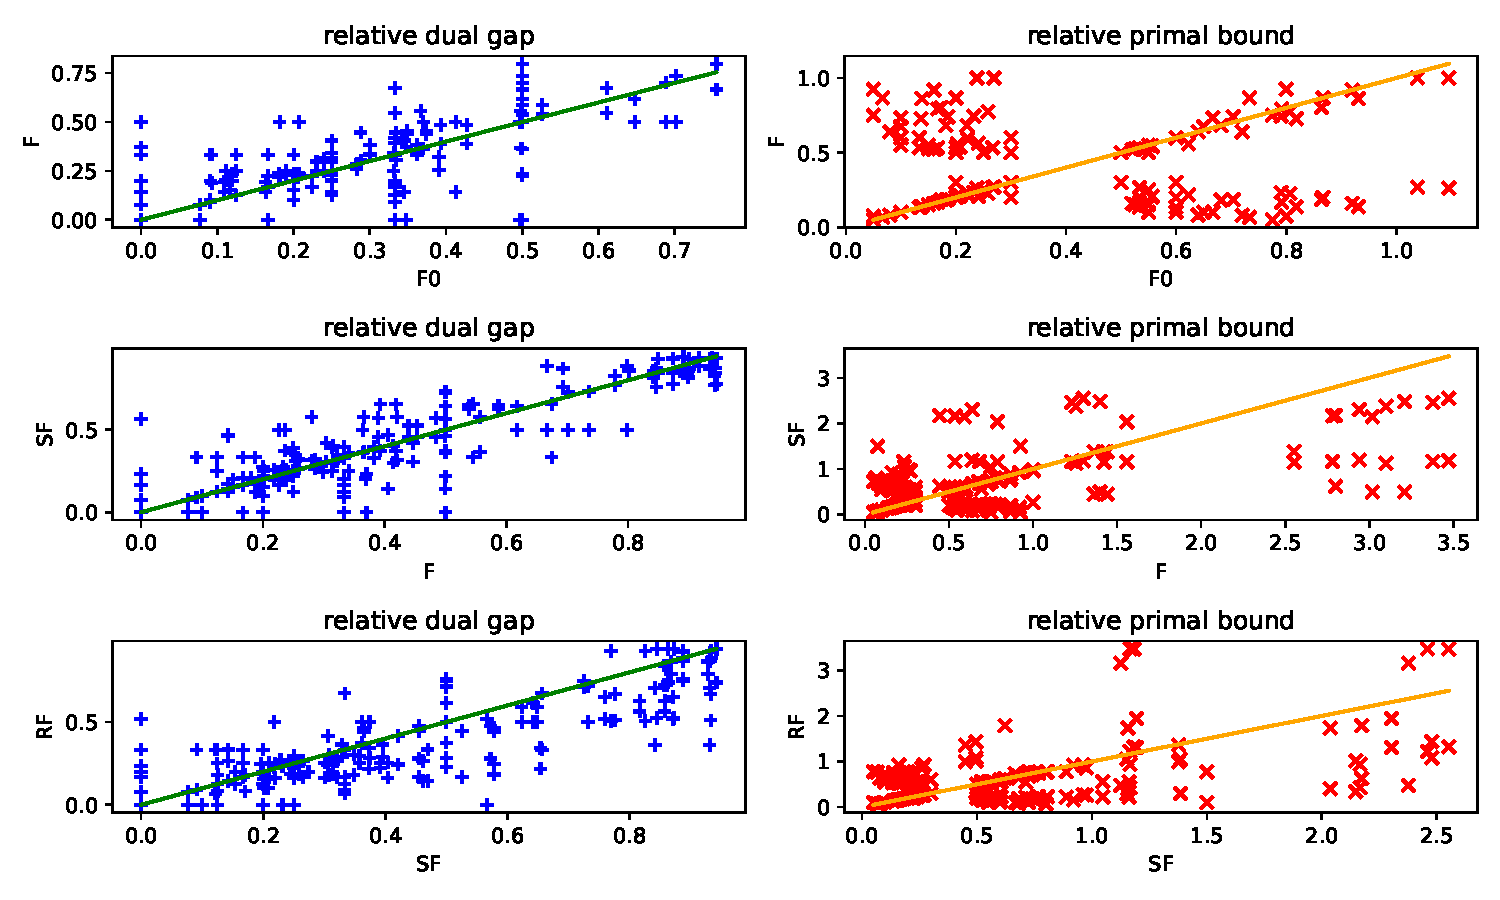
\includegraphics[width = 0.999\columnwidth]{Chaptercflg/media/scatter5.pdf}
}
\caption{Scatter plots of the relative dual gaps and the relative primal bounds between different settings}
\label{fig.scatter5}
\end{figure}

\subsection{Comparative Analysis of Continuous and Discrete Models}

 In  CSCP, the facilities are located either at nodes or edges, while in the discrete variant considered in this section facilities can only be located at nodes.
Our objective is to evaluate the number of facilities that can be saved by allowing continuous location. Since the discrete model studied here, \texttt{SFD}, is a discrete restriction of CSCP,  every optimal solution is a feasible solution of CSCP.
 We solve \texttt{SFD} for the \dfproblem \,  and compare the results with the best model for CSCP, \texttt{RF}.


In addition to the previous performance statistics, we also record for each instance, a new relative primal bound for the continuous model defined as:
$$v'_r := \frac{\overline{v}}{\overline{v_d}},$$ where $\overline{v_d}$ is the best solution found by \texttt{SFD}.  If $v'_r < 1$, then the continuous model (in this case, \texttt{RF}) finds a solution better than the one found by the discrete model.



 \begin{figure}[htbp]
\centering{
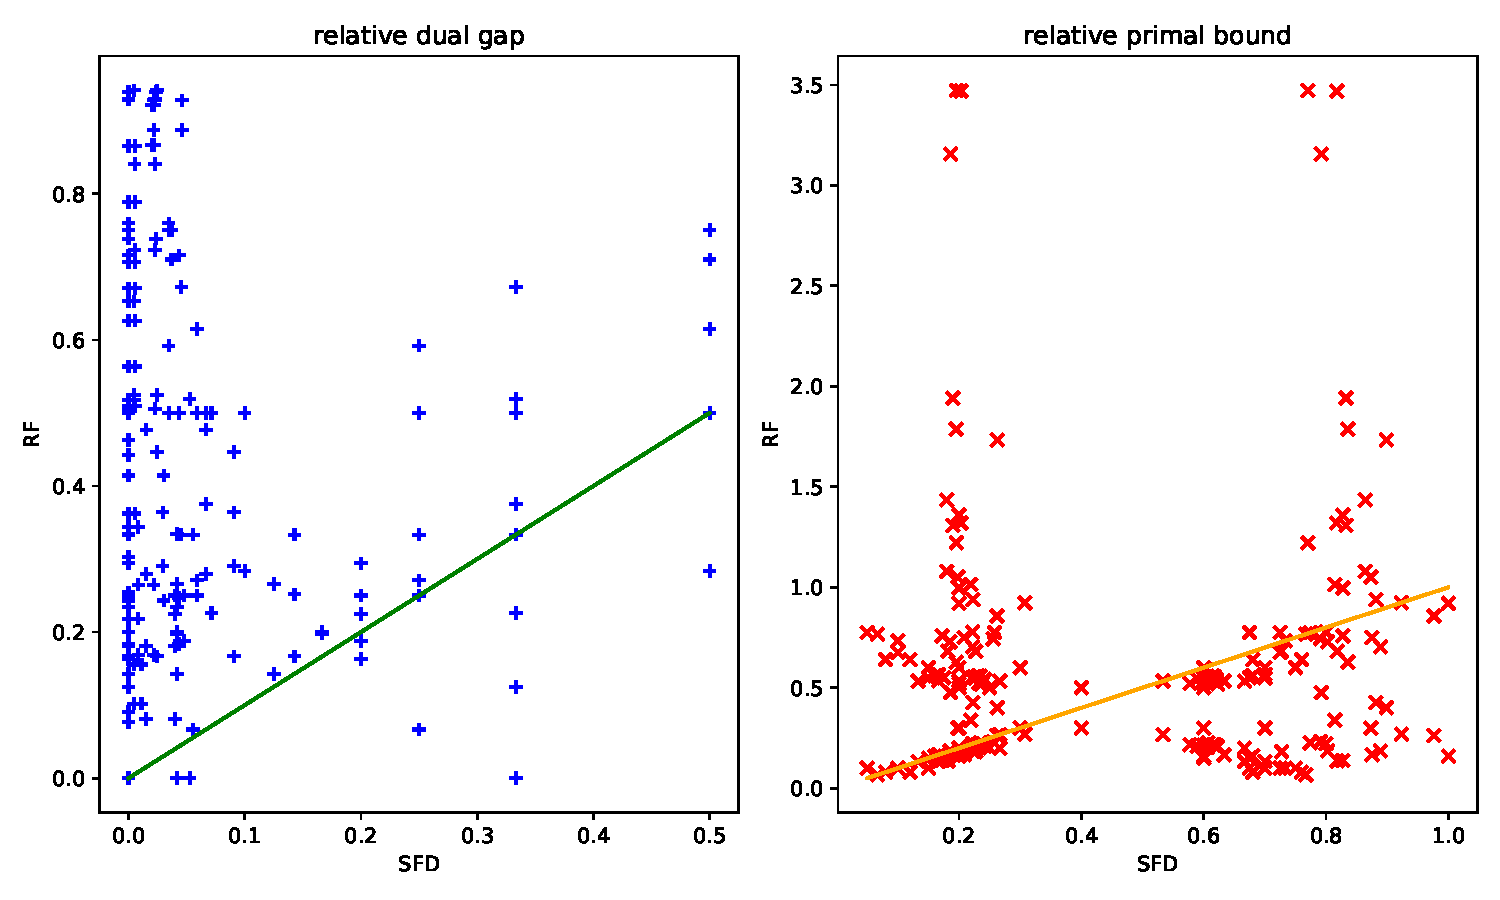
\includegraphics[width = 0.999\columnwidth]{Chaptercflg/media/scatter2.pdf}
}
\caption{Scatter plots of the relative dual gaps and the relative primal bounds between \textbf{SFD} and \textbf{RF}}
\label{fig.scatter2}
\end{figure}

\begin{table}[htbp]
\centering
\scalebox{0.75}{
\begin{tabular}{|l|l|*{5}{r}|*{5}{r}}
\hline
\multirow{2}{*}{Benchmark} & \multirow{2}{*}{Radius} & \multicolumn{5}{l|}{\texttt{RF}}                                                                                 	& \multicolumn{5}{l|}{\texttt{SFD}}                                      	\\ \cline{3-12}
                       	& & \multicolumn{1}{l|}{time} & \multicolumn{1}{l|}{$\sigma(\%)$} & \multicolumn{1}{l|}{$v_r(\%)$} &
                       	\multicolumn{1}{l|}{$v'_r(\%)$} &\multicolumn{1}{l|}{S/A/T} & \multicolumn{1}{l|}{time} & \multicolumn{1}{l|}{$\sigma(\%)$} & \multicolumn{1}{l|}{$v_r(\%)$} &
                       	\multicolumn{1}{l|}{$v'_r(\%)$} &\multicolumn{1}{l|}{S/A/T}  \\ \hline
\multirow{2}{*}{\texttt{city}}&Small & 1804.4 & 16.2\% & 54.1\% & 89.3\% & 0/9/9 & 0.2 & 0.3\% & 60.6\% & 100.0\% & \multicolumn{1}{l|}{9/9/9} \\
&Large & 1801.5 & 25.8\% & 21.3\% & 92.0\% & 0/9/9 & 3.4 & 1.1\% & 23.2\% & 100.0\% & \multicolumn{1}{l|}{9/9/9} \\ \cline{1-1}
\multirow{2}{*}{\texttt{Kgroup\_A}}&Small & 1622.6 & 21.5\% & 77.5\% & 91.1\% & 1/11/11 & 0.5 & 2.7\% & 85.1\% & 100.0\% & \multicolumn{1}{l|}{11/11/11} \\
&Large & 158.9 & 19.2\% & 19.3\% & 85.5\% & 8/11/11 & 0.4 & 6.7\% & 22.6\% & 100.0\% & \multicolumn{1}{l|}{11/11/11} \\ \cline{1-1}
\multirow{2}{*}{\texttt{Kgroup\_B}}&Small & 1800.9 & 59.1\% & 154.2\% & 185.0\% & 0/12/12 & 66.1 & 0.8\% & 83.3\% & 100.0\% & \multicolumn{1}{l|}{10/12/12} \\
&Large & 1800.6 & 75.5\% & 63.3\% & 312.1\% & 0/12/12 & 136.5 & 1.1\% & 20.2\% & 100.0\% & \multicolumn{1}{l|}{12/12/12} \\ \cline{1-1}
\multirow{2}{*}{\texttt{random\_A}}&Small & 15.9 & 8.1\% & 54.3\% & 86.0\% & 9/12/12 & 0.0 & 1.2\% & 63.2\% & 100.0\% & \multicolumn{1}{l|}{12/12/12} \\
&Large & 0.3 & 26.6\% & 19.8\% & 93.6\% & 12/12/12 & 0.0 & 2.4\% & 21.1\% & 100.0\% & \multicolumn{1}{l|}{12/12/12} \\ \cline{1-1}
\multirow{2}{*}{\texttt{random\_B}}&Small & 1304.3 & 38.5\% & 63.8\% & 91.8\% & 1/12/12 & 1.0 & 2.1\% & 69.5\% & 100.0\% & \multicolumn{1}{l|}{12/12/12} \\
&Large & 190.2 & 19.8\% & 11.2\% & 103.3\% & 9/12/12 & 1.7 & 8.7\% & 10.9\% & 100.0\% & \multicolumn{1}{l|}{12/12/12} \\ \cline{1-12}
\multirow{2}{*}{\texttt{all}}&Small & 604.9 & 23.7\% & 75.4\% & 104.6\% & 11/56/56 & 2.2 & 1.3\% & 72.1\% & 100.0\% & \multicolumn{1}{l|}{54/56/56} \\
&Large & 146.6 & 29.2\% & 22.8\% & 121.3\% & 29/56/56 & 3.9 & 3.2\% & 18.7\% & 100.0\% & \multicolumn{1}{l|}{56/56/56} \\
\cline{1-12}
\end{tabular}
}
\caption{Results for continuous and discrete models} \label{tab.cdm}
\end{table}

\Cref{tab.cdm} depicts some comparative results. A first observation is that \texttt{SFD} has fewer variables and constraints than  \texttt{RF}, as it models a simpler problem. In addition, our strengthening techniques explain that \texttt{SFD} can solve almost all instances in a very short time. Moreover, even the average relative primal bound of \texttt{SFD} is smaller than \texttt{RF}. However, we note that, with the exception of \texttt{Kgroup\_B} and \texttt{random\_B} of large radius, \texttt{RF} finds solutions with fewer facilities.  For \texttt{Kgroup\_B}, \texttt{RF} has a larger average dual gap than \texttt{SFD}.

In \Cref{fig.scatter2}, we  also show scatter plots of the relative dual gaps ($\sigma$) and the relative primal bounds ($v_r$) for those instances affected by both \texttt{SFD} and \texttt{RF}. These plots complement the averaged results of \Cref{tab.cdm} by giving information on all affected instances, and support the above analysis.

By allowing location at edges, the continuous model can reduce the number of installed facilities. However, it becomes more challenging to solve the problem. The results suggest that calling \texttt{SFD} and passing its solution as a warm-start to \texttt{RF} can make sense as a two-step optimization approach.


\section{Conclusions}\label{sec:conclu}
In this work, we use an integer programming approach to solve CSCP,  propose various MILP formulations for this problem and test these formulations against an existing MILP formulation on several benchmarks from the literature.


The existing works mainly consider discretization methods and FDS. Discretization methods are indeed preprocessing procedures that restrict CSCP to an equivalent set-covering problem with continuous demands and candidate facilities in FDS. But FDS is only computable when CSCP satisfies some assumption, so it is not practical to employ FDS  for general CSCP. On the other hand, to delimit the search space of MILP models, we use alternative preprocessing procedures. We explore the delimitation that relaxes the concept of FDS,  which also restricts the candidate space of facilities (from the full network to a still continuous sub-network).  We learn the following ideas to tackle similar problems (possibly with more complex constraints): i). Integer programming methods are more viable and flexible for general graphs, as a partial delimitation of the problems is useful for  strengthening the models (via separation of valid inequalities, tightening big-M constants, variable fixing), while the discretization methods require a full delimitation and a complete characterization of FDS. ii). Our delimitation is applicable as long as the facility location is continuous.

 Specifically, we devise and implement four models for CSCP:   \texttt{F0},  \texttt{F} and  \texttt{SF}, which belong to the same family of models, and \texttt{RF}, which is the reduced one. These models mainly differ in preprocessing procedures applied. We find that  MILP solvers cannot read or build  the MILP model from \cite{Hamacher20} for any instances in our test bed, and this is due to the model having a large number of constraints and variables. So we mainly compare our four models. We find the MILP size is the main barrier to scalability. The delimitation of those parts of the network that can be covered from a specific location has been revealed as a very effective technique to reduce the model size. In addition, avoiding breaking long edges in the reduced model also results in better scalability. In conclusion,
\texttt{RF} is the best model: it can find good solutions with a small dual gap.



Meanwhile, the model  \texttt{SF}  is easily cast into   \texttt{SFD} for the discrete restriction of CSCP. We find that allowing continuous facilities decreases the number of installed facilities but increases the solving time significantly.  We note that \texttt{SFD} finds an optimal solution for  the \dfproblem \, quickly, which is a primal solution for CSCP. Therefore, \texttt{SFD} can be called as a fast MILP-based primal heuristic for CSCP.


As for future studies, devising efficient heuristics to be integrated into MILP solvers can be useful to improve the primal performance of the proposed models. For instance, different relaxations of  CSCP can be worth exploring, such as that where demand only happens at nodes (i.e. only nodes are to be covered). Every solution of CSCP would be a solution of such relaxation, and hence the optimal value of the latter is a valid dual lower bound of the optimal value of  CSCP.  If solving this combinatorial relaxation is efficient and provides a stronger dual lower bound than the LP relaxation of CSCP, we can utilize this result and integrate the combinatorial dual bound into the MILP solver, which leads to a combinatorial branch-and-bound algorithm.



Moreover, we can investigate the potential use of FDS to further delimit the search space and integrate FDS in the preprocessing procedure.


\chapter{Conclusions and perspective}
\label{chap.con}


This chapter summarizes the key findings of this thesis. Towards the conclusion of this chapter, we delve into the perspectives of this thesis work, discussing its potential for uncovering novel applications across diverse domains and its possible avenues for further development.


\subsection{Conclusions}

Within the scope of this thesis, we focus on the examination of relaxation techniques tailored for challenging MINLP problems. Our approach revolves around a structural exploration of effective relaxation strategies suitable for a variety of problem types. In the introductory section, we introduce a comprehensive list of relaxation methods drawn from existing literature. These encompass a range of approaches, such as relaxations stemming from extended formulations, submodularity-based relaxations, PWL relaxations, and intersection cuts. Additionally, we introduce advanced relaxation techniques that build upon intersection cuts and submodularity. These relaxation tools are then employed to address various real-world applications.




Our computational findings demonstrate that enhancing relaxation methods can lead to accelerated performance in exact MINLP solvers. These enhancements are primarily effective for a specific subset of MINLP problems, given that our relaxations are tailored to the structural characteristics of such problems. Furthermore, our relaxation methods are highly adaptable, with the ability to be activated or deactivated through the structural detection functions integrated into MINLP solvers. This adaptability facilitates the seamless integration of relaxation methods within the sBB algorithmic framework. As a result, the research on MINLP becomes more accessible, as even a modest enhancement in relaxation methods can serve as a foundational component for future studies.




It is worth noting that the techniques we present primarily facilitate exact solutions for MINLP problems, albeit at the expense of increased computation time. Consequently, our relaxation methods find their ideal application in static scenarios where problems are solved offline, with a primary focus on achieving high accuracy. In such settings, these relaxation methods function as core algorithms within MINLP solvers, akin to the role of propagation in constraint programming \cite{achterberg2008constraint}. 

It is important to recognize that relaxation methods belong to a broader category of approximation methods. While relaxation methods do not directly yield solutions, approximation methods are geared towards delivering approximated solutions within a reasonable time. In this context, approximation methods are considered front-end framework, as exact MINLP solvers, commonly called upon by users instead of relaxation methods. As a result, relaxation methods can be viewed as the backends of many approximation techniques.



In recent times, the field of MINLP research has encountered several challenges arising from factors such as the emergence of deep learning techniques, the prevalence of large-scale problems, and the inherent dynamics and uncertainties present in mathematical models. Additionally, a frequently overlooked challenge for MINLP research lies in the legacy aspects of its ecosystem. In the subsequent sections, we outline two primary research directions aimed at tackling these challenges.

\section{Perspectives in algorithm design}


The historical influence of MILP techniques might contribute to the existing legacy within the MINLP ecosystem. However, the applicability of these techniques to MINLP problems is still an active research area. In the subsequent sections, we conduct a comprehensive survey of open problems and associated research perspectives. These problems expand the scope of MINLP within the wider realm of mathematical optimization.


\subsection{Extended formulations vs projected formulations}
The prevalent choice among mathematical solvers is to embrace projected formulations of the underlying relaxations, as opposed to extended formulations. This preference can be attributed to several factors. Firstly, these relaxations, notably linear programming (LP) relaxations, can be progressively enhanced by cutting planes, thus offering a straightforward means of controlling relaxation size. Secondly, it is noteworthy, that while an extended formulation with a polynomial-size may exist, it could correspond to an exponentially sized projected formulation. Nonetheless, the practical utilization of extended formulations necessitates a predetermined design to balance the trade-off involving model size and the strength of the model. An open question or ongoing debate centers around the applicability of extended formulations.


The preference over projected formulations could potentially face constraints stemming from computational resources. Given the prevailing capabilities of contemporary computers, there arises an opportunity to reevaluate the applicability of extended formulations. Recent progress in polynomial programming research has unveiled a range of attractive extended formulations, such as the sparse Lasserre hierarchy and relative entropy relaxations \cite{murray2021signomial}. These novel extended formulations introduce a degree of flexibility in representing polynomial optimization.





An approach for integrating extended formulations into solvers involves the dynamic resolution of extended formulations at specific nodes within the branch-and-bound tree. Furthermore, at a given search node, the extended formulations might be adaptively lifted, albeit at the cost of computational resources. The determination of whether to enhance these formulations is intrinsically linked to optimization theory. A comparable challenge is encountered in the context of facial reduction for semi-definite programming, which can be seen as the endeavor to identify a suitable basis for the sum-of-squares representation of a polynomial.


\subsection{Modeling power: the lack of convexity and nonlinear function types}



In the realm of MINLP, the central challenge is tackling non-convex optimization problems, although the methods deployed often hinge upon convex optimization. Particularly within the MINLP landscape, the foundational algorithmic framework rests upon the utilization of convex relaxations.

Yet, the majority of optimization solvers remain firmly rooted in LP relaxations.   Particularly, the MINLP solver Mosek can address conic programming problems. Its  reference book \cite{aps2018mosek} lists several essential cones, and the solver is capable of representing a significant portion of convex  sets through compositional operations. However, it is noteworthy that the study of these fundamental cones and their optimization attributes largely predates the 2000s. 


We aim to remain attuned to emerging application trends, uncovering novel function types that have the potential for significant impact. Pursuing this research direction has the potential to substantially expand the modeling power of solvers, enabling them to tackle a broader range of optimization challenges.

This apparent lack of basic convexity types could be attributed to the inherent lack of elementary functions - the sources of non-convexity - which include polynomial, rational, trigonometric, hyperbolic, and exponential functions, possibly including their inverse counterparts. The limitations of the available convexity forms pose a problem for the modelling power of MINLP solvers.

Most MINLP solvers can effectively handle factorizable functions and essentially work as composite functions. An ongoing research attempt is to extend their capacities to handle the demands of modern deep neural networks, which often involve a larger number of relatively simple layers. Several MINLP based approaches \cite{tsay2021partition,tjandraatmadja2020convex,zhang2023optimizing} are proposed for improving neural networks. A novel approach \cite{baudart2021pipeline,ceccon2022omlt}  addresses the challenges of progressively modeling and optimizing for auto machine learning. This perspective aligns closely with a contemporary principle in modern machine learning: the fusion of modeling and optimization. Thus, this perspective  can inspire the feature design of MINLP solvers.


Convex functions are fertile ground for ongoing research and offer numerous avenues for exploration. While conventional nonlinear functions are usually defined over scalar variables, a promising direction is to consider functions defined over cones, such as convex functions defined over positive-definite matrices. An abundance of such functions can be discovered in quantum information, since quantum states can be aptly represented by probability-dense matrices—complex positive-definite matrices with unit trace. It is worth noting, however, that despite the richness of this field, the current focus of research efforts is on efficient convex optimization techniques rather than global optimization, primarily due to the scale of dense matrices.

Our goal is to keep pace with emerging trends in applications and discover new types of features that are likely to have a significant impact. Pursuing this line of research has the potential to significantly expand the modelling power of solvers and enable them to handle a broader range of optimization tasks.

\subsection{Approximations vs. relaxations}

Throughout history, the problem domains studied in MILP and combinatorial optimization have overlapped considerably, which has fostered a continuous exchange of ideas and knowledge. One particularly common and widely used technique is that of relaxations. These relaxations act as mediators within algorithms to achieve a feasible solution.

A variety of approximation algorithms in combinatorial optimization, for example, solve relaxations to derive solutions that guarantee optimality. Many of these algorithms were developed for theoretical studies, so they guarantee worst-case performance, but in practice they may perform poorly. In contrast, in the MILP domain, relaxation methods are often integrated into the branch-and-bound search framework, with the relaxation solutions serving as the starting point for heuristics. Exact MILP solvers generally provide optimal solutions to many practical problems within a reasonable time.
It should be noted, however, that in the field of combinatorial optimization there are approximation algorithms or heuristics based on structural techniques that go beyond simple relaxation. This raises an intriguing question: Can these alternative techniques be used in the context of MINLP? For example, although there are many tailored convex optimization algorithms, convex relaxations in MINLP solvers are mainly based on primal-dual interior point solvers. Integrating these tailored algorithms to take over specific tasks in MINLP solving, such as preprocessing, could be considered as a possible research direction.

\section{Perspectives of solver framework}

The inherent legacy of the MINLP ecosystem may also stem from earlier software systems efforts. These systems, while valuable, often present challenges to new software developers and emerging researchers. The complexity associated with these systems hinders adoption of recent advances in software engineering and innovations in programming languages.
The use of the C language in mathematical optimization programs can lead experienced developers to create code with memory leaks, resulting in lengthy debugging cycles. The evolution of C++ standards leads to frequent updates and the integration of new language features in each version. However, due to the divergence between classical C and modern C++, mathematical solvers cannot benefit from these features, e.g. for efficient memory management. 


In today's programming education, the focus is on functional programming languages other than C. Consequently, the pool of new researchers who can develop tailored algorithms for MINLP may be smaller than in other areas of mathematical optimization.
A notable recent development is the SCIP team's decision to make it a fully open source protocol. This transformation raises hopes that the broader community will contribute extensively to its further development. One way to close the current gap is to gradually replace the C components of SCIP with a modern programming language. Similarly, the Linux community has begun using Rust to reimplement the Linux kernel, a strategy we can emulate.


Rust is an ahead-of-time compiled programming language that focuses on performance, type safety, and concurrency. It enforces memory safety— without requiring the use of a garbage collector or reference counting. It borrows ideas from functional programming, including static types, immutability, higher-order functions, and algebraic data types.
In addition, Rust has a built-in package management system and testing infrastructure, making it a suitable choice for an open source-driven development landscape. We envision an enriching exploration of the software framework jointly orchestrated by researchers, users, and the open source community.




%\chapter{Signed certificates for binary polynomial optimization}


\section{Problem statement}



\section{Relaxation approach}

\section{Experiments}

\section{Conclusion}


% ********************************** Back Matter *******************************
% Backmatter should be commented out, if you are using appendices after References
%\backmatter

% ********************************** Bibliography ******************************
\begin{spacing}{0.9}

% To use the conventional natbib style referencing
% Bibliography style previews: http://nodonn.tipido.net/bibstyle.php
% Reference styles: http://sites.stat.psu.edu/~surajit/present/bib.htm

\bibliographystyle{siam}
%\bibliographystyle{unsrt} % Use for unsorted references  
%\bibliographystyle{plainnat} % use this to have URLs listed in References
\cleardoublepage
\bibliography{References/references} % Path to your References.bib file


% If you would like to use BibLaTeX for your references, pass `custombib' as
% an option in the document class. The location of 'reference.bib' should be
% specified in the preamble.tex file in the custombib section.
% Comment out the lines related to natbib above and uncomment the following line.

%\printbibliography[heading=bibintoc, title={References}]


\end{spacing}

% ********************************** Appendices ********************************

\begin{appendices} % Using appendices environment for more functunality


%$\include{Appendix2/appendix2}
%%!TEX root = ../thesis.tex
% ******************************* Thesis Appendix A ****************************
\chapter{Missing proofs in \Cref{chap.sig}} 



\section*{Appendix}








\end{appendices}



% *************************************** Index ********************************
%\printthesisindex % If index is present

\backmatter
\newgeometry{left=16mm,right=16mm,top=30mm,bottom=30mm}
%%%%%%%%%%%%%%%%%%%%%%%%%%%%%%%%%%%%%%%%%%%%%%%%%%%%%%%%%%%%%%%%%%%%%%%%%%%%%%%%%%%%%%%%%%%%%%%%%%%%%%%%%%%%%%%%%%%%%%%%%%%%%%%%%%%%%%%%%%%%%%%%%%%%%%%%%%%%%%%%%%%%%%%
%%%%%%%%%%%%%%%%%%%%%%%%%%%%%%%%%%%%%%%%%%%%%%%%%%%%%%%%%%%%%%%%%%%%%%%%%%%%%%%%%%%%%%%%%%%%%%%%%%%%%%%%%%%%%%%%%%%%%%%%%%%%%%%%%%%%%%%%%%%%%%%%%%%%%%%%%%%%%%%%%%%%%%%
%%% Modèle pour la 4ème de couverture des thèses préparées à l'Institut Polytechnique de Paris, basé sur le modèle produit par Nikolas STOTT / Template for back cover of thesis made at Institut Polytechnique de Paris, based on the template made by Nikolas STOTT
%%% Mis à jour par Aurélien ARNOUX (École polytechnique)/ Updated by Aurélien ARNOUX (École polytechnique)
%%% Les instructions concernant chaque donnée à remplir sont données en bloc de commentaire / Rules to fill this file are given in comment blocks
%%% ATTENTION Ces informations doivent tenir sur une seule page une fois compilées / WARNING These informations must contain in no more than one page once compiled
%%%%%%%%%%%%%%%%%%%%%%%%%%%%%%%%%%%%%%%%%%%%%%%%%%%%%%%%%%%%%%%%%%%%%%%%%%%%%%%%%%%%%%%%%%%%%%%%%%%%%%%%%%%%%%%%%%%%%%%%%%%%%%%%%%%%%%%%%%%%%%%%%%%%%%%%%%%%%%%%%%%%%%%
%%% Version du 28 avril 2020 : utilisation de .png au lieu de .jpg pour les logos
%%%%%%%%%%%%%%%%%%%%%%%%%%%%%%%%%%%%%%%%%%%%%%%%%%%%%%%%%%%%%%%%%%%%%%%%%%%%%%%%%%%%%%%%%%%%%%%%%%%%%%%%%%%%%%%%%%%%%%%%%%%%%%%%%%%%%%%%%%%%%%%%%%%%%%%%%%%%%%%%%%%%%%%

\label{form_final}
%%%%%%%%%%%%%%%%%%%%%%%%%%%%%%%%%%%%%%%%%%%%%%%%%%%%%%%%%%%%%%%%%%%%%%%%%%%%%%%%%%%%%%%%%%%%%%%%%%%%%%%%%%%%%%%%%%%%%%%%%%%%%%%%%%%%%%%%%%%%%%%%%%%%%%%%%%%%%%%%%%%%%%%
%%%%%%%%%%%%%%%%%%%%%%%%%%%%%%%%%%%%%%%%%%%%%%%%%%%%%%%%%%%%%%%%%%%%%%%%%%%%%%%%%%%%%%%%%%%%%%%%%%%%%%%%%%%%%%%%%%%%%%%%%%%%%%%%%%%%%%%%%%%%%%%%%%%%%%%%%%%%%%%%%%%%%%%
%%% Formulaire / Form
%%% Remplacer les paramètres des \newcommand par les informations demandées / Replace \newcommand parameters by asked informations
%%%%%%%%%%%%%%%%%%%%%%%%%%%%%%%%%%%%%%%%%%%%%%%%%%%%%%%%%%%%%%%%%%%%%%%%%%%%%%%%%%%%%%%%%%%%%%%%%%%%%%%%%%%%%%%%%%%%%%%%%%%%%%%%%%%%%%%%%%%%%%%%%%%%%%%%%%%%%%%%%%%%%%%
%%%%%%%%%%%%%%%%%%%%%%%%%%%%%%%%%%%%%%%%%%%%%%%%%%%%%%%%%%%%%%%%%%%%%%%%%%%%%%%%%%%%%%%%%%%%%%%%%%%%%%%%%%%%%%%%%%%%%%%%%%%%%%%%%%%%%%%%%%%%%%%%%%%%%%%%%%%%%%%%%%%%%%%

\newcommand{\logoEd}{ed}																		%% Logo de l'école doctorale. Indiquer le sigle (EDIPP, EDMH) / Doctoral school logo. Indicate the acronym : EDMH, EDIPP
\newcommand{\PhDTitleFR}{Méthodes de relaxation pour la programmation non linéaire en nombres entiers mixtes}													%% Titre de la thèse en français / Thesis title in french
\newcommand{\keywordsFR}{Programmation non linéaire en nombres entiers mixtes, pptimisation globale, relaxation}														%% Mots clés en français, séprarés par des , / Keywords in french, separated by ,
\newcommand{\abstractFR}{\lipsum[1-3]}															%% Résumé en français / abstract in french

\newcommand{\PhDTitleEN}{Relaxation methods for mixed integer nonlinear programming}													%% Titre de la thèse en anglais / Thesis title in english
\newcommand{\keywordsEN}{Mixed-integer nonlinear programming, global optimization, relaxation}														%% Mots clés en anglais, séprarés par des , / Keywords in english, separated by ,
\newcommand{\abstractEN}{\lipsum[1-3]}															%% Résumé en anglais / abstract in english

\label{layout_final}

%%%%%%%%%%%%%%%%%%%%%%%%%%%%%%%%%%%%%%%%%%%%%%%%%%%%%%%%%%%%%%%%%%%%%%%%%%%%%%%%%%%%%%%%%%%%%%%%%%%%%%%%%%%%%%%%%%%%%%%%%%%%%%%%%%%%%%%%%%%%%%%%%%%%%%%%%%%%%%%%%%%%%%%
%%%%%%%%%%%%%%%%%%%%%%%%%%%%%%%%%%%%%%%%%%%%%%%%%%%%%%%%%%%%%%%%%%%%%%%%%%%%%%%%%%%%%%%%%%%%%%%%%%%%%%%%%%%%%%%%%%%%%%%%%%%%%%%%%%%%%%%%%%%%%%%%%%%%%%%%%%%%%%%%%%%%%%%
%%% Mise en page / Page layout      
%%% NE RIEN MODIFIER / DO NOT MODIFY
%%%%%%%%%%%%%%%%%%%%%%%%%%%%%%%%%%%%%%%%%%%%%%%%%%%%%%%%%%%%%%%%%%%%%%%%%%%%%%%%%%%%%%%%%%%%%%%%%%%%%%%%%%%%%%%%%%%%%%%%%%%%%%%%%%%%%%%%%%%%%%%%%%%%%%%%%%%%%%%%%%%%%%%
%%%%%%%%%%%%%%%%%%%%%%%%%%%%%%%%%%%%%%%%%%%%%%%%%%%%%%%%%%%%%%%%%%%%%%%%%%%%%%%%%%%%%%%%%%%%%%%%%%%%%%%%%%%%%%%%%%%%%%%%%%%%%%%%%%%%%%%%%%%%%%%%%%%%%%%%%%%%%%%%%%%%%%%
{
\thispagestyle{empty}
{\fontsize{9.2pt}{11.04pt}\selectfont
%%% Logo de l'école doctorale. Le nom du fichier correspond au sigle de l'ED / Doctoral school logo. Filename correspond to doctoral school acronym
%%% Les noms valides sont / Valid names are : EDMH, (EDIPP)
\tekstblokkulur{white}
\begin{textblock*}{61mm}(16mm,3mm)
	\noindent
\includegraphics[height=24mm]{media/ed/EDIPP.png}
\end{textblock*}



%%%Titre de la thèse en français / Thesis title in french
\begin{center}
\fcolorbox{black}{white}{\parbox{0.95\textwidth}{
{\bf Titre:} Méthodes de relaxation pour la programmation non linéaire en nombres entiers mixtes
\medskip

%%%Mots clés en français, séprarés par des ; / Keywords in french, separated by ;
{\bf Mots clés:} PNLNE; optimisation globale ; relaxation
\vspace{-2mm}

%%% Résumé en français / abstract in french
\begin{multicols}{2}
{\bf Résumé:} 
Cette thèse se concentre sur la programmation non linéaire à variables mixtes (MINLP), une classe de problèmes d'optimisation mathématique, et les algorithmes associés pour les résoudre. L'algorithme central utilisé dans de nombreux solveurs d'optimisation globale pour les problèmes MINLP est l'algorithme  de séparation et évaluation. La clé du succès de l'algorithme  de séparation et évaluation réside dans l'utilisation de relaxations des problèmes d'optimisation, qui sont essentielles pour obtenir des bornes duales efficaces.
Cependant, la construction de relaxations efficaces dépend des structures spécifiques des problèmes d'optimisation. Dans la première partie de cette thèse, nous présentons un aperçu complet des outils de relaxation structurelle adaptés aux problèmes MINLP structurés liés à
différents domaines d’applications. Ces outils englobent des relaxations à partir de formulations étendues, des relaxations par sous-modularité, des relaxations utilisant une approximation linéaire par morceaux et des renforcements de relaxation via des coupes d'intersection. Nous développons de nouveaux résultats théoriques avancés basés sur ces outils. Dans la deuxième partie, nous utilisons ces techniques de relaxation pour aborder divers problèmes d'optimisation. Nous explorons les plans coupants pour la programmation signoïdale. Nous proposons des coupes d'intersection pour améliorer les relaxations  linéaire des problèmes d'optimisation sous-modulaire.
Nous étudions les relaxations de Dantzig-Wolfe pour un problème de programmation linéaire à variables mixtes dans le routage de réseaux sans fil et un problème MINLP dans le binpacking sous-modulaire. Enfin, nous étudions la technique de relaxation big-M appliquée aux fonctions linéaires par morceaux dans le problème de couverture continue sur un réseau. 
Les travaux réalisés durant cette thèse de doctorat contribuent à l’avancement des approches de la programmation non linéaire en nombre entiers et des méthodes d’optimisation connexes.
En effet la combinaison des études exhaustives réalisées sur diverses techniques de relaxation et leurs applications à différents contextes d’optimisation offrent des perspectives précieuses tant pour la compréhension théorique des problèmes que pour la mise en œuvre empirique des résultats.
\end{multicols}
}}
\end{center}

\vspace*{0mm}

%%%Titre de la thèse en anglais / Thesis title in english
\begin{center}
\fcolorbox{black}{white}{\parbox{0.95\textwidth}{
{\bf Title:} Relaxation methods for mixed-integer
nonlinear programming
\medskip

%%%Mots clés en anglais, séprarés par des ; / Keywords in english, separated by ;
{\bf Keywords:}  MINLP; global optimization; relaxation %%3 à 6 mots clés%%
\vspace{-2mm}
\begin{multicols}{2}
	
%%% Résumé en anglais / abstract in english
{\bf Abstract:} 
This thesis focuses on mixed-integer nonlinear programming (MINLP), a class of mathematical optimization problems, and the associated algorithms to solve them. The core algorithm utilized in many global optimization solvers for MINLP problems is the branch-and-bound algorithm. Key to the success of the branch-and-bound approach is the use of relaxations of optimization problems, which are vital in obtaining efficient and tight dual bounds.
However, constructing effective relaxations depends on the specific structures of optimization problems. In the first part of this thesis, we present a comprehensive overview of structural relaxation tools tailored for structured MINLP problems across different disciplines.  These tools encompass relaxations from extended formulations, relaxations via submodularity, relaxations using piece-wise linear approximation, and  relaxation tightening via intersection cuts. Then, we develop novel advanced theoretical results based on these tools. In the second part, we  employ these relaxation techniques to address various optimization problems. We explore cutting planes for signomial programming. Then, we propose intersection cuts for enhancing linear programming relaxations of submodular optimization problems.
Next, we investigate the Dantzig-Wolfe  relaxations for a mixed-integer linear programming problem in wireless network routing and a MINLP problem in submodular binpacking. Finally, we study the big-M relaxation technique as applied to piece-wise linear functions in the continuous covering problem on a network.  
By combining these comprehensive studies on various relaxation techniques and their applications in different optimization contexts, this thesis contributes to the advancement of MINLP and related optimization methods, offering valuable insights for both theoretical understanding and computational implementation.
\end{multicols}
}}
\end{center}

\tekstblokkulur{white}
\begin{textblock*}{161mm}(10mm,270mm)
{\bf\noindent Institut Polytechnique de Paris	         }

\noindent
\noindent 91120 Palaiseau, France 
\end{textblock*}

\tekstblokkulur{white}
\begin{textblock*}{20mm}(175mm,265mm)

\includegraphics[width=20mm]{media/IPPARIS-petit}
\end{textblock*}

}
}

\restoregeometry

\end{document}
